%%%%%%%%%%%%%%%%%%%%%%%% Springer-Verlag
\documentclass[epjST]{svjour}

\usepackage{amsmath,amssymb}
\usepackage{float}
\usepackage{imakeidx}
\usepackage[colorlinks=true,linkcolor=blue,citecolor=blue,urlcolor=magenta]{hyperref}
\usepackage[framemethod=TikZ]{mdframed}
\usepackage{footnote}
\usepackage{comment}
\usepackage{doi}
\usepackage{enumitem}
\usepackage{slashed}
\usepackage{xcolor}
\usepackage{xstring}
\usepackage{xparse}
%\usepackage[numbers,authoryear]{natbib}
\usepackage{graphicx}
\usepackage{rotating}
\usepackage{aastex_hack}
\usepackage{appendix}
\makeindex

% Draft number lines on pages
\usepackage{lineno}
\linenumbers

\makesavenoteenv{tabular}
\makesavenoteenv{table}
\makesavenoteenv{figure}

% Make Orcid icon
\newcommand{\orcidicon}{\includegraphics[width=0.32cm]{orcid.pdf}}
\newcommand{\orc}[1]{\href{https://orcid.org/#1}{\orcidicon}}

% Author Orcid ID: Define per author
\newcommand{\orcA}{0000-0001-8217-1484}
\newcommand{\orcB}{0000-0001-5038-8427}
\newcommand{\orcC}{0000-0001-5474-2649}
\newcommand{\orcD}{0000-0003-2704-6474}
\newcommand{\orcE}{0000-0002-2289-4856}
\newcommand{\orcF}{0000-0001-9985-1822}

% Useful macros for equations and units
\newcommand{\ts}{\textstyle}
\newcommand*{\TeV}{\text{\,TeV}}
\newcommand*{\GeV}{\text{\,GeV}}
\newcommand*{\MeV}{\text{\,MeV}}
\newcommand*{\keV}{\text{\,keV}}
\newcommand*{\eV}{\text{\,eV}}
\newcommand*{\meV}{\text{\,meV}}
\newcommand*{\Msun}{\mathrm{M}_{\odot}}
\newcommand*{\bb}{\boldsymbol}
\newcommand*{\beqn}{\begin{equation}}
\newcommand*{\eeqn}{\end{equation}}
\newcommand{\beql}[1]{\begin{equation} \label{#1}}
\newcommand{\eeql}[1]{\label{#1} \end{equation} }  
\newcommand{\req}[1]{Eq.\,(\ref{#1})}
\newcommand{\rf}[1]{Fig.\,{\ref{#1}}}
\newcommand{\rt}[1]{Table~{\ref{#1}}}
\newcommand{\rsec}[1]{Sec.\,{\ref{#1}}}
\newcommand{\rchap}[1]{Ch.\,{\ref{#1}}}
\newcommand{\rapp}[1]{Appendix~{\ref{#1}}}
\newcommand{\mydoi}[2]{\href{http://dx.doi.org/#2}{#1}}
\newcommand{\E}{\mathrm{e}}
\newcommand{\ie}{{\em i.e.\/}}  
\newcommand{\eg}{{\em e.g.\/}}  
\newcommand{\ms}[1]{\rule[-#1mm]{0mm}{0mm}}
\newcommand{\grad}{\operatorname{grad}}
\newcommand{\diag}{\mathrm{diag}}

% Andrew's commands
\newcommand{\cccite}[1]{\textit{Published in Ref.~\cite{#1} under the \href{https://creativecommons.org/licenses/by/4.0/}{CC BY 4.0} license}}
\newcommand{\radapt}[1]{\textit{Adapted from Ref.~\cite{#1}}}
\newcommand{\para}[1]{\paragraph{#1}\hfill\break\noindent}
\NewDocumentCommand{\allcite}{m o}{\nocite{#1}\hyperlink{cite.#1}{\StrBefore{#1}{:}\IfNoValueTF{#2}{ et. al. }{ and #2 }(\StrBehind{#1}{:}[\temp]\StrLeft{\temp}{4})}}
\NewDocumentCommand{\aucite}{m o}{\nocite{#1}\hyperlink{cite.#1}{\StrBefore{#1}{:}\IfNoValueTF{#2}{ }{ and #2 }(\StrBehind{#1}{:}[\temp]\StrLeft{\temp}{4})}}
\NewDocumentCommand{\allcitep}{m o}{\nocite{#1}\hyperlink{cite.#1}{\StrBefore{#1}{:}\IfNoValueTF{#2}{ et. al. }{ and #2 }(preprint \StrBehind{#1}{:}[\temp]\StrLeft{\temp}{4})}}

% Chris's commands
%\newcommand{\reff}[1]{Figure\,({\ref{#1}})}
\newcommand{\wt}[1]{\widetilde{#1}}
\newcommand{\eq}[1]{#1^{(\mathrm{eq})}}
\newcommand{\peq}[1]{#1^{'(\mathrm{eq})}}
\newcommand{\reqs}[2]{Eqs.\,({\ref{#1}}-{\ref{#2}})}
\newcommand{\mk}{|\boldsymbol{k}|}
\newcommand{\ft}[1]{\widetilde{\boldsymbol{#1}}}
\newcommand{\hatv}[1]{\hat{\boldsymbol{#1}}}
\newcommand{\angstrom}{\textup{\AA}}

% Struts for tables 
\newcommand\Tstrut{\rule{0pt}{2.6ex}}
\newcommand\Bstrut{\rule[-0.9ex]{0pt}{0pt}}
\newcommand{\TBstrut}{\Tstrut\Bstrut}

% Equations numbered by section
\numberwithin{equation}{section}

\begin{document}
%%%%%%%%%%%%%%%%%%%%%%%% 
%\title{Quarks to Cosmos: Particles and Plasma in\\ 
 Cosmological evolution}

\author{
Johann Rafelski${}^1$\orc{\orcA}\thanks{Corresponding author 
\email{johannr@arizona.edu}}, 
Jeremiah Birrell${}^{1,2}$\orc{\orcE}, 
Christopher Grayson${}^1$\orc{\orcF}, 
\newline Andrew Steinmetz${}^1$\orc{\orcC}, 
Cheng Tao Yang${}^1$\orc{\orcB}
}

\institute{${}^1$Department of Physics, The University of Arizona, Tucson, AZ, 85721, USA\\
${}^2$Department of Mathematics, Texas State University, San Marcos, TX, 78666, USA}

\abstract{\vspace{-0.25cm}We describe in the context of the particle physics (PP) standard model (SM) `PP-SM' the understanding of the primordial properties and composition of the Universe in the temperature range $130\GeV>T>20\keV$. The Universe evolution is described using FLRW cosmology. We present a global view on particle content across time and describe the different evolution eras using deceleration parameter $q$. In the considered temperature range the unknown cold dark matter and dark energy content of $\Lambda\mathrm{CDM}$ have a negligible influence allowing a reliable understanding of physical properties of the Universe based on PP-SM energy-momentum alone. We follow the arrow of time in the expanding and cooling Universe: After the PP-SM heavies $(t, h, W, Z)$ diminish in abundance below $T\simeq 50\GeV$, the PP-SM plasma in the Universe is governed by the strongly interacting Quark-Gluon content. Once the temperature drops below $T\simeq 150\MeV$, quarks and gluons hadronize into strongly interacting matter particles comprising a dense baryon-antibaryon content. Rapid disappearance of baryonic antimatter ensues, which adopting the present day photon-to-baryon ratio completes at $T_\mathrm{B}=38.2\MeV$. We study the ensuing disappearance of strangeness and mesons in general. We show that the different eras defined by particle populations are barely separated from each other with abundance of muons fading out just prior to $T=\mathcal{O}(2.5)\MeV$, the era of emergence of the free-streaming neutrinos. We develop methods allowing the study of the ensuing speed of the Universe expansion as a function of fundamental coupling parameters in the primordial epoch. We discuss the two relevant fundamental constants controlling the decoupling of neutrinos. We subsequently follow the primordial Universe as it passes through the hot dense electron-positron plasma epoch. The high density of positron antimatter disappears near $T=20.3\keV$, well after the Big-Bang Nucleosynthesis era: Nuclear reactions occur in the presence of a highly mobile and relatively strongly interacting electron-positron plasma phase. We apply plasma theory methods to describe the strong screening effects between heavy dust particle (nucleons). We analyze the paramagnetic characteristics of the electron-positron plasma when exposed to an external primordial magnetic field.}
\maketitle
%%%%%%%%%%%%%%%%%%%%%%%%%%%%%%%%%%%%%%%
\newpage
\setcounter{tocdepth}{3}
\tableofcontents
%%%%%%%%%%%%%%%%%%%%%%%%%%%%%%%%%%%%%%%

%%%%%%%%%%%%%%%%%%%%%%%%%%%%%%%%%%%%%%% 
\section{Introduction}
%%%%%%%%%%%%%%%%%%%%%%%%%%%%%
\subsection{Theoretical models of the primordial Universe}\label{ssec:UniLab}
In this report we explore the connection between particle, nuclear, and plasma physics in the evolution of the Universe. Our work concerns the domain described by the known laws of physics as determined by laboratory experiments.

Our journey in time through the expanding primordial Universe has the objective of understanding how different evolution eras impact each other. We are seeking to gain deeper insights into the fundamental processes that shaped our cosmos, by providing a clearer picture of the Universe's origin and its ongoing expansion. The question we address is how a very hot soup of elementary matter evolves and connects to the normal matter present today, indirectly observed by the elemental ashes of the Big-Bang nucleosynthesis (BBN)\index{Big-Bang!BBN}. 

{\color{black}In this report we report on our  ongoing work on particle and plasma cosmology. Our aim is to create a continuous description of the primordial Universe spanning and connecting different particle and plasma epochs. This allows the reader to understand the physics spanning the entire temperature domain we explore, $130\GeV>T>20\,\mathrm{keV}$. We will define many topics deserving further study: There are many open questions to which this work provides an introduction.}

{\color{black}This manuscript is not a traditional review, as its focus is on our own ongoing work: We aim here to offer a readable report describing and explaining what can appear at times to be a fragmented body of work. A  guide- and time-line how our theoretical insights were gained over the past dozen years is presented in \rapp{list:Works}.}

{\color{black}As appropriate we highlight in \rapp{list:Works} the key results and provide fields of application not yet fully explored. This helps to create a backdrop of knowledge and introduces further areas of study potentially helping to understand the primordial Universe and sharpen prediction of observable quantities today.} 

%%%%%%%%%%%%%%%%%%%%%%%
\para{Dominance of visible radiation and matter in the primordial Universe}
In this report, we aim to connect various eras of cosmological evolution which can be addressed with some confidence in view of the already known particle and nuclear properties as measured experimentally. By analyzing the primordial Universe as a function of time in~\rf{fig:energy:frac} we are exploring the role of particle physics standard model (PP-SM) in the Universe evolution. We snapshot in this report specific epochs in the primordial Universe, and/or on specific physical conditions such as primordial magnetic fields.

%%%%%%%%%%%%%%%%%%%%%%%%%%%%%%%%%%%%
\begin{sidewaysfigure}
\vspace*{0.62\linewidth}\includegraphics[width=\linewidth]{plots/energyFractions.pdf}\label{fig:energy:frac}
\caption{Evolving in time fractional energy composition of the Universe. See text for discussion. \cccite{Rafelski:2023emw}. \radapt{Birrell:2014ona}.}
 \end{sidewaysfigure}
%%%%%%%%%%%%%%%%%%%%%%%%%%%%%%%%%%

In the cosmic epoch considered here with temperature above $kT=20\keV$, the present day dominant dark matter and dark energy played a negligible role in the cosmos. The changing energy component composition of the Universe\index{Universe!composition} is illustrated in~\rf{fig:energy:frac}. To create the figure we integrate the Universe backwards in time. The initial condition is the assumed composition of the Universe in the current era: $69\%$ dark energy, $26\%$ dark matter, $5\%$ baryons\index{baryon}, while photons and neutrinos comprise less than one percent. We further assumed one massless neutrino and two with $m_\nu=0.1$\,eV. Other neutrino mass values are possible; constraints remain weak\index{neutrino!mass}. How this solution is obtained will become evident at the end of~\rsec{sec:flrw} below. 

As described, there are two unknown dark components as one is able to disentangle these given two independent inputs in the cosmic energy-momentum tensor of homogeneous isotropic matter, pressure and energy density, which can be related by equations of state. The current epoch cosmic accelerated expansion (Nobel price 2011 to Saul Perlmutter, Adam Riess, and Brian P. Schmidt -- a graduate also in physics at The University of Arizona) creates the need for this two component ``darkness''.\index{Universe!darkness}

Dark energy in the conventional definition is akin to $\Lambda$=Einstein's cosmological term. $\Lambda$ is a fixed property of the Universe and does not scale with temperature. In comparison, radiation energy content scales with $T^4$ and is vastly dominant in the temperature range we explore; the dark energy (black line) emerges in a very recent past (on logarithmic time scale, see~\rf{fig:energy:frac}. Cold, {\it i.e.\/}, massive on temperature scale,  dark matter (CDM) content scales with $T^{3/2}$ for $m/T\gg 1$. In the temperature regime of interest to us CDM (blue line in~\rf{fig:energy:frac}) complements the invisible normal baryonic matter (purple line). Both are practically invisible in the Universe inventory in the epoch we explore, emerging just after as a $10^{-5}$ energy fraction shown~\rf{fig:energy:frac}. The further back we look at the hot Universe, the more irrelevant become all forms of matter, including the ``dark'' matter component.\index{Universe!radiation dominated} 

There is considerable tension\index{Hubble parameter!tension} between studies determining the present day speed of cosmic expansion (Hubble parameter)~\cite{DiValentino:2024spr,DiValentino:2021izs}: Extrapolation from more distant past, looking as far back as is possible, {\it i.e.\/}, the recombination epoch near redshift $z=1000$, are smaller than the Universe properties observed and studied in the current epoch. This result stated often asking the question ``$h_0=0.67$ or $0.73$?'' about contemporary Hubble parameter\index{Hubble parameter} $H_0(=100\,h_0$\,(km/Mpc)/s). This unresolved issue arises comparing diverse epochs when the Universe was in its atomic, molecular, stellar forms. One would think that therefore this discrepancy is in principle irrelevant to our particle and plasma study of the primordial Universe. 

However, as we will argue this separation of scales may not be complete. Depending on the details of PP-SM unobserved contents, {\it e.g.\/}, in the neutrino sector, free-streaming not quite massless quantum neutrinos contribute to darkness and may impact the result of extrapolation (``$h_0=0.67$ or $0.73$?'') of the Hubble expansion from recombination epoch to the current epoch. One could argue that the effort to study the ``Unknown'' darkness in cosmology suffers from the lack of the full understanding of the ``Known'' in the primordial cosmos which masquerades as darkness today. This is one of the many motivations for the research effort we pursue. 

%%%%%%%%%%%%%%%%%%%%%%%%%%%%%%%%%%%%%%%%%%
\para{Cosmic plasma in the primordial Universe}
We use units in which the Boltzmann constant $k_\mathrm{B}=1$. In consequence, the temperature $T$ is discussed in this report in units of energy either MeV $\simeq 2 m_{\rm e} c^2$ ($m_{\rm e}$ is the electron mass) or GeV$= 1000$ MeV $\simeq m_{\mathrm N} c^2$ ($m_{\rm N}$ is the mass of a nucleon) or as the Universe cools in keV, one-thousandth of an MeV. The conversion of an MeV to temperature familiar units involves ten additional zeros. This means that when we explore hadronic matter at the `low' temperature: 
\begin{equation} \label{tempval}
100\MeV\equiv 116\times 10^{10}\,\mathrm{K}\, ,
\end{equation}
we exceed the conditions in the center of the Sun at $T=11\times 10^6$\,K by a factor of 100\,000. 

 
The primordial hot Universe fireball underwent several nearly adiabatic phase changes that dramatically evolved its bulk plasma properties as it expanded and cooled. {\color{black} The periods near to a major structural change include the Electro-weak phase transition, QGP hadronization, neutrino decoupling, BBN nucleosynthesis, and development of cosmological scale magnetic fields. These transitions all require the development and/or application of nonequilibrium kinetic theory methods. These boundaries connect the different epochs in the history of the Universe. This report is dedicated to the study of these non-equilibrium transitions which require from the reader the full mastery of the thermal equilibrium conditions we also describe.}

We begin in the temperature range below temperature of electro-weak (EW) boundary at $T=130\GeV$, when massive elementary particles emerged in the electro-weak symmetry broken phase of matter. {\color{black}The cosmic plasma in the primordial Universe evolves within the first hour down to the temperature of about $T\simeq 10\keV$ where this report will end. We will address the four well separated domains of particle plasma all visible by inspection of~\rf{fig:energy:frac}, connect these and extend our study to the two topical cosmological challenges, the BBN and cosmological magnetic field development.}

Notable plasma epochs include:\index{Universe!plasma epochs} 
%$300\MeV >T>0.02\MeV$ ~\cite{Rafelski:2023emw}.
\begin{enumerate}
\item \textbf{Primordial quark-gluon plasma epoch:} 
At early times when the temperature was between $130\GeV>T>0.15\GeV$ we have in the primordial plasma in their thermal abundance all PP-SM building blocks of the Universe as we know them today, including the Higgs particle, the vector gauge electroweak and strong interaction bosons, all three families of leptons and free deconfined quarks: For most of the evolution of QGP all hadrons\index{QGP!hadronization} are dissolved into their constituents $u,d,s,t,b,c,g$. However, as temperature decreases below heavy particle mass, the thermal abundance is much reduced but is in general expected to remain in abundance (chemical) equilibrium due to the presence of strong interactions. \\[0.2cm]
%
However, we will show in~\rsec{Bottom} that near to the QGP phase transition $300\, \mathrm{MeV}>T>150\MeV$, the chemical equilibrium\index{chemical equilibrium} of the bottom quark\index{bottom quark} abundance is broken. The abundance described by the fugacity parameter relatively slowly diminishes, see~\rf{fugacity_bc}, with only a small deviations from stationary state detailed balance, see~\rf{NonFugacity}. The expansion of the Universe through the epoch of the bottom quark abundance disappearance from the particle inventory provides us the arrow of time often searched for, but never found in the current epoch\index{arrow of time}.\\[0.2cm]
%
For general reference we establish the energy density near to the end of the QGP epoch in the Universe by considering a benchmark value at $T\simeq 150\MeV$
\begin{equation} \label{endensval}
%%%\epsilon=1\ \mathrm{GeV fm}^{-3}= 1.8\ \mathrm{x}\ 10^{15}\,\mathrm{g/cc}.
\epsilon=1\,\mathrm{GeV/fm}^3
= 1.8\times 10^{15}\,\mathrm{g\,cm^{-3}} 
=1.8\times 10^{18}\,\mathrm{kg m^{-3}}\,.
\end{equation}
The corresponding relativistic matter pressure converted into human environment unit is
\begin{equation} \label{presval}
P\simeq \ts\frac{1}{3} \epsilon=0.52\times 10^{30} \,\mathrm{bar}\,.
\end{equation}
%
\item \textbf{Hadronic epoch:} Near the Hagedorn temperature\index{Hagedorn!temperature} $T_H\approx 150\MeV$, a phase transformation occurred, forcing the free quarks and gluons to become confined within baryons\index{baryon} and mesons; experimental results confirming the universal nature of the hadronization process were described in Ref.\,\cite{Letessier:2005qe}. In the temperature range $ 150\MeV >T>20\MeV$, the Universe is rich in physical phenomena involving strange mesons and (anti)baryons including long lasting (anti)hyperon abundances~\cite{Fromerth:2012fe,Yang:2021bko}. The antibaryons\index{baryon!antibaryon} disappear from the Universe inventory at temperature $T=38.2\MeV$. However, strangeness remains in the inventory down to $T\approx13\MeV$. The detailed balance assures that the weak decay is compensated by inverse reactions, see~\rsec{Strangeness} for detailed discussion.
%
\item \textbf{Lepton-photon epoch:} For temperature $10\MeV >T>2\MeV$, massless leptons and photons controlled the fate of the Universe: The Universe contained relativistic electrons, positrons, photons, and three species of (anti)neutrinos. During this epoch Massive $\tau^\pm$ disappear from the plasma at high temperature via decay processes. However, $\mu^\pm$ leptons can persist in the primordial Universe until temperature $T=4.2\MeV$.\\[0.2cm]
%
In this temperature epoch neutrinos were still coupled to the charged leptons via the weak interaction~\cite{Birrell:2014ona,Birrell:2012gg}, they freeze-out in the temperature range $3\MeV >T>2\MeV$, exact value depends on the neutrino's flavors and the magnitude of the PP-SM parameters, see~\rsec{Neutrino} for detailed discussion. After neutrino freeze-out, they still play a important role in the Universe expansion via the effective number of neutrinos\index{neutrino!effective number} $N_{\nu}^{\mathrm{eff}}$, which relates to the Hubble parameter value in the current epoch.
%
\item \textbf{Electron-positron epoch:} After neutrinos freeze-out at $T=3\sim 2\MeV$ and become free-streaming in the primordial Universe, the cosmic plasma was dominated by electrons, positrons, and photons. In the $e^+e^-$ plasma, positrons $e^+$ persisted in similar to electron $e^-$ abundance until the temperature $T=20.3\keV$, see~\rsec{Electron} for detailed discussion. Properties of this plasma need to be studied in order to understand the behavior of the nucleon dust dynamics including:
%
\item \textbf{BBN in the midst of the ${\mathbf e^+e^-}$ plasma:}\index{Big-Bang!BBN} Contrary to what was the prevailing context only a few years ago, today it is understood that BBN occurred within a rich electron-positron $e^+e^-$ plasma environment. There are thousands if not millions of ${ e^+e^-}$-pairs for each nucleon undergoing nuclear fusion reactions during the BBN epoch. 
%
\item \textbf{Primordial magnetism:}\index{magnetic!primordial fields} The $e^{+}e^{-}$-pair plasma at temperatures reaching well below BBN epoch in the primordial Universe could be an origin of the present day intergalactic magnetic fields~\cite{Rafelski:2023emw,Steinmetz:2023nsc}. In~\rsec{Electron} we present a detailed discussion of our model: We explore Landau diamagnetic and magnetic dipole moment paramagnetic properties. A relatively small magnitude of the $e^{+}e^{-}$ magnetic moment polarization asymmetry suffices to produce a self-magnetization in the Universe consistent with present day observations. In \rsec{chap:QCD} we present the theoretical developments needed for 
\end{enumerate}

{\color{black} However, the origin of primordial magnetic fields remains unknown. The further back in time that origin could be traced, the stronger the magnetic field will be due to cosmological scaling described in~\rsec{Electron} . It is well possible that the primordial origin could occur when the QGP filled the Universe. We prepare for this possibility that connects directly with the ongoing relativistic heavy ion collision studies by presenting in~\rsec{chap:QCD} the current understanding of the QGP phase in the presence of strong magnetic fields in a linear response model.}

After $e^+e^-$ annihilation finishes at a temperature near 20.3\,keV, the Universe was still opaque to photons due to large photon-electron scattering Thompson cross section. Observational cosmology study of the Cosmic Microwave Background\index{CMB} (CMB)~\cite{Planck:2018vyg} addresses the visible epoch beginning after free electron binding into atoms -- a process referred to as recombination (clearly better called atom-formation). This is complete and the Universe becomes visible to optical experiments at $T_\mathrm{recomb}\approx 0.25\,\mathrm{eV}$. 

%%%%%%%%%%%%%%%%%%%%%%%%%%%%%%%%%
\para{Toward experimental study of primordial particle Universe} Just before quarks and gluons were adopted widely as elementary degrees of freedom in PP-SM, the so-called `Lee-Wick' model of dense primordial matter prompted a high level meeting: The Bear Mountain November 29-December 1, 1974 symposium had a decisive impact on the development of the research program leading to the understanding of primordial particles in the Universe. This meeting was not open to all interested researchers: Only a few dozen were invited to join the participant club, see last page of the meeting report:\index{Bear Mountain!1974 Symposium} \url{https://www.osti.gov/servlets/purl/4061527}. This is an unusual historical fact witnessed by one of us (JR), for further discussion see Ref.\,\cite{Rafelski:2019twp}.\index{Bear Mountain!symposium}

It is noteworthy that our report appears in essence on the 50th-year anniversary of this 1974 meeting and is accompanied by the passing of the arguably the most illustrious symposium participant, T.D.\,Lee (passed away August 4, 2024 at nearly 98\index{Lee-Wick!dense matter}). Within just half a century the newly developed PP-SM knowledge has rendered all but one insight of the 1974 meeting obsolete: The participating representatives of particle and nuclear physics elite of the epoch recognized the novel opportunity to experimentally explore hot and dense hadron (strongly interacting) matter by colliding high energy nuclei (heavy-ions); the initial objective was the discovery of the Lee-Wick super dense matter but the objectives evolved rapidly in following years. One of the symposium participants, Alfred Goldhaber, planted in the Nature magazine~\cite{Goldhaber:1978qp} the seed which grew into the RHIC collider at BNL-New York. 

%%%%%%%%%%%%%%%%%%%%%%%%%%%%%%%%%
\para{Phase transformation in the primordial Universe} Thanks to the tireless effort of Rolf Hagedorn~\cite{Rafelski:2016hnq}\index{Hagedorn}, the European laboratory CERN\index{CERN} was intellectually well positioned to embark on the rapid development of related physics ideas and the required experimental program. The preeminent physics motivation that soon emerged was the understanding of the primordial composition of the hot Universe. The pre-1970 idea advanced by Hagedorn, by Huang and Weinberg~\cite{Huang:1970iq} and in the following by many others, was that the Universe was bound to the maximum Hagedorn temperature of $kT\le kT_H=150-180\MeV$ at which the energy content diverged\index{Universe!maximum Hagedorn temperature}. In the following years and indeed by the time of the Bear Mountain meeting the idea that a symmetry restoring change in phase structure at finite temperature was already taking hold~\cite{Weinberg:1974hy,Harrington:1974fc}, unnoticed by the limited in scope Bear Mountain crowd.

Today we understand Hagedorn temperature $T_H$\index{Hagedorn!temperature} to be the phase transformation to the deconfined phase of matter where quarks and gluons can exist. The first clear statement about the existence of such a phase boundary connecting the Hagedorn hadron gas phase\index{hadrons!gas phase} with the constituent quarks and gluons, and invoking deconfinement at high temperature, was the 1975 work of Cabibbo and Parisi~\cite{Cabibbo:1975ig}. This was followed by a more quantitative characterization within the realm of the MIT bag model by~\cite{Chin:1978gj} and soon after by Rafelski and Hagedorn incorporating Hagedorn bootstrap model of hadronic matter with finite size hadrons melting into QGP, see Ref.\,\cite{Rafelski:2015cxa} and appendices A and B therein. This work implemented Cabibbo-Parisi proposal as well as it was at that time possible.

Could deconfined state of a hot phase of quarks and gluons we call QGP really exist beyond Hagedorn temperature? A broad acceptance of this new insight took decades to take hold. For some, this was natural. In 1992 Stefan Pokorski asked ``What else could be there?'' when one of us (JR) was struggling to convince the large and skeptical academic course crowd at the Heisenberg-MPI in Munich. Those who were like Pokorski convinced that QCD state of matter prevails in the 1970's and 1980's epoch missed the need to smoothly connect quarks to hadrons, or as we say in the title of this work, quarks to cosmos\index{Quarks!to cosmos}, and do this incorporating gluons. 

Neglecting or omitting the gluonic degrees of freedom pushed the transformation temperature in the Universe towards $T=400\MeV$, creating a glaring conflict with the well established Hagedorn hadronic phase temperature limit $T_H\simeq 160\pm 10\MeV$. Yet other large body of work in this epoch addressed the dissolution at ultra high density and {\bf zero temperature} of hadrons into quark constituents, a process of astrophysical interest, without relevance to the understanding of both the the primordial Universe and of dynamic phenomena observed in relativistic heavy-ion collisions\index{heavy-ion!collisions}.

The present day understanding of the primordial QGP Universe was for some reason out of context for most nuclear scientists of the epoch, while to some of us the key issues became clear within less than a decade. Arguably the first Summer School connecting quarks to cosmos and relativistic heavy-ion laboratory experiments was held in the Summer 1992 under the leadership of Hans Gutbrod and one of us (JR) in the small Italian-Tuscan resort Il Ciocco. The following is the abstract of the forward article {\it Big-Bang in the Laboratory}\index{Big-Bang} of the proceedings volume presented more than 30 years ago~\cite{Gutbrod1993}: 

\begin{quote}
`Particle Production in Excited Matter' (the title of the proceeding volume, and of the meeting) happened at the beginning of our Universe. It is also happening in the laboratory when nuclei collide at highly relativistic energies. This topic is one of the fundamental research interests of nuclear physics of today and will continue to be the driving force behind the accelerators of tomorrow. In this work we are seeking to deepen the understanding of the history of time. Unlike other areas of Physics, Cosmology, the study of the birth and evolution of the Universe has only one event to study. But we hope to recreate in the laboratory a state of matter akin to what must have been a stage in the evolution when nucleons were formed. This occurred not too long after the Big-Bang birth of the Universe, when the disturbance of the vacuum made appear an extreme energy density leading to the creation of particles, nucleons, atoms and ultimately nebulas and stars. Figure 1 depicts the evolution of the Universe as we understand it today. On the left-hand scale is shown the decrease of the temperature as a function of time shown on the right side. The cosmological eras associated with the different temperatures and sizes of the Universe are described in between.
\end{quote}

Indeed! Today the ongoing laboratory work at CERN-LHC\index{CERN!LHC} and BNL-RHIC\index{BNL!RHIC} exploring the physics of QGP in the high temperature and high particle density regime reached in relativistic heavy-ion collisions allows us to study elementary strongly interacting matter connecting quarks to the cosmos. These two fields, primordial Universe and ultra relativistic heavy-ion collisions relate to each other very closely. There is little if any relation to the other, dense neutron matter research program. Such matter is found in compact stars; super-novae explosions create at much different matter density temperatures reaching 50\,MeV. 

%%%%%%%%%%%%%%%%%%%%%%%%%%%%%%%%%%%%%%%%%%%%
\para{Comparing Big-Bang with laboratory micro-bang}
The heavy-ion collision micro-bang involves time scales many orders of magnitude shorter compared to the characteristic scale governing the Universe Big-Bang: The expansion time scale of the Universe is determined by the interplay of the gravitational force and the energy content of the hot matter, whereas in the micro-bangs there is no gravitation to slow the explosive expansion.\index{heavy-ion!micro-bang} The initial energy density is reflecting on the nature of strong interactions, and the lifespan of the micro-bang is a fraction of $\tau_\mathrm{MB}\le 10^{-22}$\,s, the time for particles to cross at the speed of light the localized fireball of matter generated in relativistic heavy-ion collision. 

It is convenient to represent the Universe expansion time constant\index{Universe!expansion at hadronization} $\tau_{\mathrm U}$ as the inverse of the Hubble parameter\index{Hubble parameter} at a typical ambient energy density $\rho_0$
\beql{taudef}
\tau_{\mathrm U} \equiv \frac{1}{H[\rho_0=1\,\mathrm{GeV/fm^3}]}=14\,\mu\mathrm{s}
\,.
\eeqn
The Universe is indeed expected to be about 15 orders of magnitude slower in its expansion compared to the exploding micro-bang fireball formed in collisions of relativistic heavy-ion laboratory experiments. 

Above, the value of $\rho_0$ is chosen in the context of the `freezing' of deconfined QGP into hadrons\index{QGP!hadronization} in primordial Universe near to $T_0\simeq 150\MeV$: The strongly interacting degrees of freedom contribute as measured in laboratory relativistic heavy-ion collisions about half to this value, $\rho_h\simeq 0.5\,\mathrm{GeV/fm^3}$; the other half is the contribution of neutrinos, charged leptons, and photons. The fact that these two energy density components are nearly equal is implicit in many results shown in the following, see for example~\rf{EntropyDOF:Fig}: At hadronization we have twice as many (entropic) degrees of freedom than will remain in the radiation dominated Universe once hadrons disappear.

We obtain the relation between $H$ and $\rho$ by remembering one of the fundamental relations in the Friedmann-Lema{\^i}tre-Robertson-Walker (FLRW)\index{cosmology!FLRW} cosmology, the so-called Hubble equation\index{Hubble!equation}
\beql{Hubble:eq}
H^2=\frac{8\pi G_N}{c^2}\,\frac{\rho}{3}=
c^2 \frac{\hbar c}{M_p^2c^4} \,\frac{\rho}{3}
\,.
\eeqn
We introduced here and will use often the Planck mass\index{Planck!mass} $M_p$, defined in terms of $G_N$
\beql{eq:GN}
\frac{1}{c^4}8\pi G_N\equiv \frac{\hbar c}{M_p^2c^4}\,, \qquad 
M_p c^2=2.4353\, 10^{18}\GeV\,.
\eeqn
This definition of $M_p$, while more convenient in cosmology, differs by the factor $1/\sqrt{8\pi}$ from the particle physics convention introduced by particle data group (PDG)~\cite{ParticleDataGroup:2022pth}
\beql{eq:MplPDG}
 \sqrt{8\pi} M_p c^2 \equiv M_p^\mathrm{PDG} c^2 =1.2209\, 10^{19}\GeV\,.
\eeqn

The difference between the ``two bangs'' (heavy-ion and the Universe) due to the very different time scales involved is difficult to resolve. The evolution of the Universe is slow on the hadronic reaction time scale. Given the value of characteristic $\tau_{\mathrm U}$ we obtained, we expect that practically all unstable hadronic particles evolve to fully attain equilibrium, with ample time available to develop a `mixed phase' of QGP and hadrons, and for electromagnetic and even weak interactions to take hold generating complete particle equilibrium. All this can not occur during the life span of the dense matter created in relativistic nuclear-collisions. To understand the Universe based on laboratory experiments running at a vastly different time scale, we must therefore use theoretical models as developed in this report.\index{Big-Bang!micro-bang comparison}

There are other notable differences between the laboratory fireball and the cosmic primordial plasma. The primordial quark-hadron Universe was practically baryon\index{baryon} free comparing the net (less antibaryon) baryon number to cosmic backgrounds of remnant particles. The residual asymmetry level was and remains at $10^{-9}$. In the laboratory micro-bang at the highest CERN-LHC energy,\index{CERN!LHC} we create a fireball of dense matter with a net baryon number per total final particle multiplicity at a fraction of a percent. This matter-antimatter-abundance asymmetry between laboratory and primordial Universe is easily overcome theoretically, since it implies a relatively minor extrapolation. Any small abundance of baryons can be an experimental diagnostic signal for QGP but not a key feature of the matter produced.

%%%%%%%%%%%%%%%%%%%%%%%%%%%%%%%%%%%%%%%%%%%
\para{Can QGP be discovered experimentally?}
This takes us right to the question: Can we really tell apart in these explosive ultra relativistic heavy-ion experiments the two different phases of strongly interacting matter, the deconfined quark gluon plasma and `normal', confined strongly interacting matter? Existence of these two distinct phases is a new paradigm that superseded the Hagedorn singularity at the Hagedorn temperature. In the laboratory, the outcome of ultra-relativistic heavy-ion collisions\index{heavy-ion!collisions} seems to be very much the same irrespective of the applicable paradigm, we achieve the conversion of the kinetic energy of colliding nuclei into many material particles. So is a transient deconfined QGP phase really formed in relativistic heavy collisions? This question haunted this field of research for decades~\cite{Rafelski:2015cxa,Harris:2024aov}, a topic which is not addressed in this work beyond the following few words: 

When one of us (JR) first arrived at CERN in 1977, he found himself immersed into ardent discussions about both what the structure of the hot primordial Universe could be, and if indeed we could figure out how to find the answer in an experiment. Was the Universe perhaps a dense baryon-antibaryon singular Hagedorn Universe? Or was indeed the confinement condition not really retained at high temperature~\cite{Weinberg:1974hy,Harrington:1974fc,Cabibbo:1975ig}? And, above all, how can we tell these models apart doing laboratory experiments? By 1979 it became clear that new experimental ideas and a new observable was needed, sensitive to specific properties of the dense deconfined hot matter if formed in experiments. Strange antibaryon\index{baryon!antibaryon} enhancement was one of the proposed novel approaches and in the opinion of one of us (JR); this was to be later the decisive QGP discovery evidence~\cite{Rafelski:2019twp}.\index{quark-gluon plasma!signature}


%%%%%%%%%%%%%%%%%%%%%%%%%%%%%%%%%%%%%%%%%%%%%%
\subsection{Concepts in equilibrium statistical physics} \label{sec:statphys}
We now recall the fundamental statistical physics concepts necessary to explore the properties of the Universe during its 'first hour'. {\color{black} We begin by considering the laws of equilibrium thermodynamics which provide a framework for understanding the behavior of particle's energy density, pressure, number density and entropy in the Universe. These expressions presume local thermal equilibrium which prevailed in the relatively slowly expanding Universe.}

We will address the general Fermi and Bose distributions\index{Bose!distribution}\index{Fermi!distribution} and its application in the primordial Universe, as well as the cases of special interest to thermodynamics in the primordial Universe. We describe partial freeze-out conditions, {\it i.e.\/}, rise of the chemical nonequilibrium abundance, while kinetic scattering equilibrium is maintained, and the case of free-streaming particles, allowing for switching from radiation like to massive nonrelativistic condition. In the following we use natural units\index{natural units} $c=\hbar=k_\mathrm{B}=1$. While we have shown  $c$ and $\hbar$ explicitly before, we have measured temperature in units of energy, thus implicitly taking $k_\mathrm{B}T\to T$, {\it i.e.\/}, $k_\mathrm{B}=1$.

%%%%%%%%%%%%%%%%%%%%%%%%%%%%%
\para{Quantum statistical distributions}
\index{statistical distribution}
In the primordial Universe, the reaction rates of particles in the cosmic plasma were much greater than the Universe expansion rate $H$. Therefore, the local thermal equilibrium was in general maintained. Assuming the particles are in thermal equilibrium, the dynamical information about local energy density can be estimating using he single-particle quantum statistical distribution function. The general relativistic covariant Fermi/Bose momentum distribution can be written as
\begin{align}
f_{F/B}(\Upsilon_i,p_i)=\frac{1}{\Upsilon^{-1}_i\exp{\left[(u\cdot p_i-\mu_i)/T\right]}\pm1}
\,,
\end{align}
where the plus sign applies for fermions, and the minus sign for bosons. The Lorentz scalar $(u_i\cdot p_i)$ is a scalar product of the particle four momentum $p^\mu_i$ with the local four vector of velocity $u^\mu$. In the absence of local matter flow, the local rest frame is the laboratory frame 
\begin{align}
u^\mu=\left(1,\vec{0}\right),\,\,\,\,\,\,\,\,\, p^\mu_i=\left(E_i,\vec{p}_i\right)\,.
\end{align} 
The parameter\index{fugacity} $\Upsilon_i$\index{Bose!distribution} is the fugacity of a given particle characterizing the pair density and it is the same for both particles and antiparticles. For $\Upsilon_i=1$, the distribution maximizes the entropy content at a fixed particle energy, this maximum is not very pronounced~\cite{Letessier:1993qa}. The parameter $\mu_i$ is the chemical potential\index{chemical potential} for a given particle which is associated to the density difference between particles and antiparticles.

%%%%%%%%%%%%%%%%%%%%%%%%%%
\para{Chemical equilibrium}
In general there are two types of chemical equilibrium\index{chemical equilibrium} associated with the chemical parameters $\Upsilon$ and $\mu$ each. We have:
\begin{itemize}
\item \underline{\it Absolute chemical equilibrium:\/} 
The absolute chemical equilibrium is the level to which energy is shared into accessible degrees of freedom, \eg\ the particles can be made as energy is converted into matter.
The absolute equilibrium is reached when the phase space occupancy approaches unity $\Upsilon\to1$. 
 \item \underline{\it Relative chemical equilibrium:\/}
 The relative chemical equilibrium is associated with the chemical potential $\mu$ which involves reactions that distribute a certain already existent element/property among different accessible compounds. 
 \end{itemize}
The dynamics of absolute chemical equilibrium, in which energy can be converted to and from particles and antiparticles, is especially important. The consequences for the energy conversion to from particles/antiparticle can be seen in the first law of thermodynamics by introducing the chemical potential $\mu_N$ for particle and $\mu_{\bar{N}}$ for antiparticle as follows:
\begin{align}
\mu_N\equiv\mu+T\ln\Upsilon,\qquad{\mu_{\bar{N}}}\equiv{-\mu}+T\ln\Upsilon.
\end{align}
Then the first law of thermodynamics can be written as
\begin{align}
dE&=-PdV+TdS+{\mu_N}dN+{\mu_{\bar{N}}}d{\bar{N}}
\\&=-PdV+TdS+{\mu}(dN-d{\bar{N}})+T\ln{\Upsilon}(dN+d{\bar{N}}).
\end{align}
Here the chemical potential\index{chemical potential}\index{fugacity} $\mu$ is the energy required to change the difference between particles and antiparticles, and $T\ln\Upsilon$ is the energy required to change the total number of particles and antiparticles; the fugacity $\Upsilon$ is the parameter allowing to adjust this energy.

%%%%%%%%%%%%%%%%%%%%%%%%%%%%%%%%%
\para{Boltzmann equation and particle freeze-out}
The Boltzmann equation describes the evolution of {\color{black} a (nonequilibrium)} distribution function $f$ in phase space. General properties of the Boltzmann-Einstein equation\index{Boltzmann-Einstein equation} in an arbitrary spacetime are explored in~\rsec{sec:BoltzmannEinstein}. The Boltzmann equation in the FLRW\index{cosmology!FLRW} Universe takes the Einstein-Vlasov form\index{Einstein-Vlasov equation}
\begin{align}\label{Hubble:Boltzmann}
\frac{\partial f}{\partial t}-\frac{\left(E^2-m^2\right)}{E}H\frac{\partial f}{\partial E}=\frac{1}{E}\sum_{i}\mathcal{C}_i[f]\,,
\end{align}
where $H=\dot{a}/a$\index{Einstein-Vlasov equation!Hubble expansion} is the Hubble parameter\index{Hubble parameter},~\req{dynamic}, see~\rsec{sec:flrw} below for a more detailed cosmology primer. Due to the homogeneity and isotropy of the Universe, the distribution function depends on time $t$ and energy $E=\sqrt{p^2+m^2}$ only. The collision term $\sum_i \mathcal{C}_i$ represents all elastic and inelastic interactions and the index $i$ labels the corresponding physical process. In general, the collision term is proportional to the relaxation time for a given collision as follows~\cite{Anderson:1974nyl}
\begin{align}
\frac{1}{E}\mathcal{C}_i[f]\propto\frac{1}{\tau_\mathrm{rel}}\,,
\end{align}
where $\tau_\mathrm{rel}$ is the relaxation time for the reaction, which characterizes the magnitude of the reaction time to reach chemical equilibrium. 

As the Universe expands, the collision term in the Boltzmann equation competes with the Hubble term. In general, a given particle freezes-out from the cosmic plasma when its interaction rate $\tau_\mathrm{rel}^{-1}$ becomes smaller than the Hubble expansion rate\index{freeze-out}
\begin{align}
H\geqslant\tau_\mathrm{rel}^{-1}.
\end{align}
When this happens, the particle's interactions are not rapid enough to maintain thermal distribution, either because the density of particles becomes so low that the chance of any two particles meeting each other becomes negligible, or because the particle energy becomes too low to interact. The freeze-out process can be categorized into three distinct stages based on the type of freeze-out interactions, we have~\cite{Birrell:2012gg,Rafelski:2023emw}:
\begin{itemize}
\item \underline{\it Chemical freeze-out:\/}\index{freeze-out!chemical} 
As the Universe expands and the temperature drops, the rate of the inelastic scattering (\eg\ production and annihilation reaction) that maintains the equilibrium density becomes smaller than the expansion rate. At this point, the inelastic scattering ceases, and a relic population of particles remain. Prior to the chemical freeze-out temperature, number changing processes are significant and keep the particle in thermal equilibrium, implying that the distribution function has the usual Fermi-Dirac\index{Fermi!distribution} form 
\begin{equation}\label{equilibrium}
f_\mathrm{ch}(t,E)=\frac{1}{\exp[(E-\mu)/T]+1},\qquad \text{ for } T(t)> T_\mathrm{ch}
\,,
\end{equation}
where $T_\mathrm{ch}$ represents the chemical freeze-out temperature. \\[-0.2cm]
%
\item \underline{\it Kinetic freeze-out:\/}\index{freeze-out!kinetic}
After chemical freeze-out, at yet lower temperature in an expanding Universe particles still scatter elastically from other particles and keep thermal equilibrium in the primordial plasma. As the temperature drops, the rate of elastic scattering reaction that maintain the thermal equilibrium become smaller than the expansion rate. At that time, elastic scattering processes cease, and the relic particles do not interact with other particles in the primordial plasma anymore; they free-stream. 

Once chemical freeze-out takes hold, the distribution function has the kinetic equilibrium\index{kinetic equilibrium} form with pair abundance typically below maximum yield~$\Upsilon \le 1$
\begin{equation}\label{kinetic:equilibrium}
f_\mathrm{k}(t,E)=\frac{1}{\Upsilon^{-1}\exp[(E-\mu)/T]+1},\qquad \text{ for }T_k< T(t)< T_\mathrm{ch},
\end{equation}
where $T_k$ represents the kinetic freeze-out temperature. The generalized fugacity\index{fugacity} $\Upsilon(t)$ controls the occupancy of phase space and is necessary once $T(t)<T_\mathrm{ch}$ in order to conserve the particle number. {\color{black} In general we encounter $T_k<T_{\mathrm{ch}}$ allowing us to denote the complete thermal and kinetic freeze-out temperature as $T_\mathrm{F}\simeq T_k$: for $T< T_\mathrm{F}$ all scattering becomes negligible for the considered particle species.}\\[-0.2cm]
%
\item \underline{\it Free streaming:\/}
{\color{black}After freeze-out at $T<T_\mathrm{F}$, all particles have fully decoupled from the primordial plasma and become free-streaming\index{free-streaming}. They ceased influencing the dynamics of the Universe  other than by their gravity contributing  to the energy-momentum tensor. Therefore, the free-streaming momentum distribution follows from the non-interacting  Einstein-Vlasov momentum evolution equation, see \req{VEeqFLR}.  This equation} can be solved~\cite{Choquet-Bruhat:2009xil} as we describe in \rsec{sec:model:ind},  and the free-streaming momentum distribution can be exactly given\index{Einstein-Vlasov equation} as~\cite{Birrell:2012gg}\index{free-streaming!quantum distribution}
\begin{equation}\label{freeStreamDist}
f_\mathrm{fs}(t,E)=\frac{1}{\Upsilon^{-1}\exp{\left[\sqrt{\frac{E^2-m^2}{T_\mathrm{fs}^2}+\frac{m^2}{T^2_\mathrm{F}}}-\frac{\mu}{T_\mathrm{F}}\right]+1}}\,,
\quad T_\mathrm{fs}(t)=\frac{a(t_F)}{a(t)}\,T_\mathrm{F}\,,
\end{equation}
{\color{black}where $t_F$ is the time at which full freeze-out occurs. The free-streaming effective temperature $T_\mathrm{fs}$ is obtained by redshifting the temperature at kinetic freeze-out as shown.}\\[0.2cm] 
%
Considering a massive particle (\eg\ dark matter) freeze-out process from cosmic plasma in the nonrelativistic regime, $m\gg T_\mathrm{F}$. We can use the
Boltzmann\index{Boltzmann!approximation} approximation, and the free-streaming distribution for nonrelativistic particle becomes
\begin{align}\label{freeStreamDistNR}
&f^B_\mathrm{fs}(t,p)=\Upsilon\,e^{-(m+\mu)/T_\mathrm{F}}\exp\left[-\frac{1}{ T_\mathrm{eff}}\frac{p^2}{2m}\right],\quad T_\mathrm{eff}=\left(\frac{a(t_\mathrm{F})}{a(t)}\right)^2T_\mathrm{F}\,,
\end{align}
where we note the effective temperature $T_\mathrm{eff}$ for massive free-streaming particles: The effective temperature for massive particles decreases faster than the Universe temperature cools. The difference in temperatures between cold free-streaming particles and hot cosmic plasma is worth emphasizing. How this would affect the evolution of the primordial Universe requires more detailed study. 
\end{itemize}

The division of the freeze-out process into these three regimes is a simplification of much more complex overlapping dynamical processes. It is, however, a very useful approximation in the study of cosmology~\cite{Rafelski:2023emw,Birrell:2012gg,Mangano:2005cc,Birrell:2014gea}.

%%%%%%%%%%%%%%%%%%%%%%%%%%%%%%%%%%%%%% 
\para{Particle content of the Universe} 
Our detailed understanding of the primordial Universe arises from half a century of research in the fields of cosmology, ultra relativistic heavy-ion collisions, particle, nuclear and plasma physics. Today we believe that the primordial deconfined matter we call quark-gluon plasma (QGP) filled the entire Universe and lasted for about first $20\,\mathrm{\mu s}$ after the Big-Bang~\req{taudef}\index{Big-Bang}. The deconfined condition allows free motion of quarks and gluons along with all other elementary particles. 

This hot primordial particle soup filled the expanding Universe as long as it was well above hadronization\index{QGP!hadronization} Hagedorn temperature\index{Hagedorn!temperature} $T_H\simeq 150\MeV$. Well below $T\ll T_H$, the Universe contained all the building blocks of the usual matter that surrounds us today. Depending on the temperature, many other elementary matter particles could also be present as seen in \rf{fig:energy:frac}. The total particle inventory thus includes:
\begin{itemize}
\item The up $u$ and down $d$ quarks now hidden in protons and neutrons;
\item Electrons, and  three flavors  of (Majorana) neutrinos;\\[-0.2cm]
%
\item[] There were also unstable particles present which can decay but are reformed in hot Universe:\\[-0.2cm]
%
\item Heavy unstable leptons muon $\mu$ and tauon $\tau$;
\item Unstable when bound in present day matter strange $s$, and heavy charm $c$ and bottom $b$ quarks;\\[-0.2cm]
%
\item[] At yet higher temperatures unreachable in laboratory experiments today we encounter all the remaining much heavier standard model particles:\\[-0.2cm]
% 
\item Electroweak theory gauge bosons W$^\pm$ and Z$^0$, the top $t$ quark, and the Higgs particle H.
\item The QGP phase of matter contains also the gluons, particles mediating the strong interaction of deconfined quarks.
\end{itemize}

Using the relativistic covariant Fermi/Bose momentum distribution, the corresponding energy density $\rho_i$\index{particle!energy density}, pressure $P_i$\index{particle!pressure}, and number densities $n_i$\index{particle!density} for particle species $i$ and mass $m_i$ are given by
\begin{align}
\rho_i&=g_i\int\!\!\frac{d^3p}{(2\pi)^3}Ef_{F/B}=\frac{g_i}{2\pi^2}\!\int_{m_i}^\infty\!\!\!dE\,\frac{E^2\left(E^2-m_i^2\right)^{1/2}}{\Upsilon_i^{-1}e^{(E-\mu_i)/T}\pm 1}\,,
\label{energy_density}\\[0.2cm]
P_i&=g_i\int\!\!\frac{d^3p}{(2\pi)^3}\frac{p^2}{3E}f_{F/B}=\frac{g_i}{6\pi^2}\!\int_{m_i}^\infty\!\!\!dE\,\frac{\left(E^2-m_i^2\right)^{3/2}}{\Upsilon_i^{-1} e^{(E-\mu_i)/T}\pm 1}\,,
\label{Pressure_density}\\[0.2cm]
n_i&=g_i\int\!\!\frac{d^3p}{(2\pi)^3}f_{F/B}=\frac{g_i}{2\pi^2}\!\int_{m_i}^\infty\!\!\!dE\,\frac{E(E^2-m_i^2)^{1/2} }{\Upsilon_i^{-1}e^{(E-\mu_i)/T}\pm 1}\,,
\label{number_density}\\[0.2cm]
\sigma_i=&-g_i\int\!\! \frac{d^3p }{(2\pi)^3}(f_{F/B}\ln(f_{F/B})\pm(1\mp f_{F/B})\ln(1\mp f_{F/B}))
\,,
\end{align}
where $g_i$ is the degeneracy of the particle species `$i$'. Inclusion of the fugacity parameter $\Upsilon_i$ allows us to characterize particle properties in chemical nonequilibrium situations. 

{\color{black}Given the above relations for the energy density $\rho_i$, pressure $P_i$, and number densities $n_i$, the entropy density $\sigma_i$\label{entropy_density} for particle species $i$ of mass $m_i$ can be obtained by integration by parts leading to the usual Gibbs–Duhem form}\index{entropy!density}
\begin{align}\label{entropy}
\sigma_i=\frac{S_i}{V}=\frac{\partial P_i}{\partial T}=\left(\frac{\rho_i+P_i}{T}-\frac{\tilde \mu_i}{T}\,n_i\right)\,,\qquad
n_i=\frac{\partial P_i}{\partial \tilde{\mu}_i}\,,\qquad
\tilde \mu_i=T\ln \Upsilon_i +\mu_i\,,
\end{align}
where the chemical potential associated with charge, baryon number, etc., changes sign between particles and antiparticles, while $\Upsilon_i$ does not.

Once full decoupling is achieved, the corresponding free-streaming energy density, pressure, number density and entropy arising from the solution of the Boltzmann-Einstein equation\index{Boltzmann-Einstein equation} differ from the thermal equilibrium \req{energy_density}, \req{Pressure_density}, \req{number_density}, and~\req{entropy} by replacing the mass by a time dependant effective mass $m\,T_\mathrm{fs}(t)/T_\mathrm{F}$ in the exponential, and other related changes which will be derived in~\rsec{sec:model:ind}, see \req{eq:NeutrinoRho}, \req{eq:NeutrinoP}, \req{eq:NumDensity}, and \req{eq:EntropyIntegrand}. Once decoupled, the free-streaming particles maintain their comoving number and entropy density, see~\req{eq:ConstEntropy}.

In general the chemical potential is associated with the baryon number. The net baryon number density relative to the photon number density\index{baryon!per photon ratio} is near to $10^{-9}$. In many situations we can neglect the small chemical potential when calculating the total entropy density\index{entropy!density} in the Universe. The total entropy density in the primordial Universe can be written as
\begin{align}\label{eq:entg}
&\sigma=\sum_i\,\sigma_i=\frac{2\pi^2}{45}g^s_\ast\,T^3,\\
&g^s_\ast=\sum_{i=\mathrm{bosons}}g_i\left({\frac{T_i}{T_\gamma}}\right)^3B\left(\frac{m_i}{T_i}\right)+\frac{7}{8}\sum_{i=\mathrm{fermions}}g_i\left({\frac{T_i}{T_\gamma}}\right)^3F\left(\frac{m_i}{T_i}\right),\label{eq:entg002}
\end{align}
where $g^s_\ast$ counts the effective number of `entropy' degrees of freedom. The functions $B(m_i/T)$ and $F(m_i/T)$ are defined as \index{entropy!degrees of freedom}
\begin{align}
&B\left(\frac{m_i}{T}\right)=\frac{45}{12\pi^4}\int^\infty_{m_i/T}\,dx\sqrt{x^2-\left(\frac{m_i}{T}\right)^2}\left[4x^2-\left(\frac{m_i}{T}\right)^2\right]\frac{1}{\Upsilon^{-1}_ie^x-1},\\
&F\left(\frac{m_i}{T}\right)=\frac{45}{12\pi^4}\frac{8}{7}\int^\infty_{m_i/T}\,dx\sqrt{x^2-\left(\frac{m_i}{T}\right)^2}\left[4x^2-\left(\frac{m_i}{T}\right)^2\right]\frac{1}{\Upsilon^{-1}_ie^x+1}.
\end{align}
In~\rf{EntropyDOF:Fig} we show $g^s_\ast$ as a function of temperature, the effect of particle mass threshold~\cite{Coc:2006rt} is considered in the calculation for all considered particles. When $T$ decreases below the mass of particle $T\ll m_i$, this particle species becomes nonrelativistic and the contribution to $g^s_\ast$ becomes negligible, creating the smooth dependence on $T$ across mass threshold seen in~\rf{EntropyDOF:Fig}: The vertical lines identify particle mass thresholds on temperature axis, $m_e=0.511\MeV$, $m_\mu=105.6\MeV$, and pion average mass $m_\pi\approx138\MeV$.

%%%%%%%%%%%%%%%%%%%%%%%%%
\begin{figure} 
\centerline{\includegraphics[width=0.9\linewidth]
%{./plots/DOF_entropy.jpg}
{./plots/g_entropy.jpg}}
\caption{The entropy degrees of freedom as a function of $T$ in the primordial Universe epoch after hadronization $10^{-2}\MeV \leqslant T \leqslant 150 \MeV$. \radapt{Yang:2024ret}.}
\label{EntropyDOF:Fig} 
\end{figure}
%%%%%%%%%%%%%%%%%%%%%%%%%%%%% 

%%%%%%%%%%%%%%%%%%%%%%%%%%%%%
\para{Departure from detailed balance}
A well-known textbook result for the case of two particle scattering is that the Boltzmann scattering term, the right-hand side in~\req{Hubble:Boltzmann}, vanishes when particles reach thermal equilibrium. The rates of the forward and reverse reactions are equal, resulting in a balance between production and annihilation of particles. Such a balance is called detailed balance\index{detailed balance}. Thermal equilibrium implies both chemical equilibrium\index{chemical equilibrium} (particle abundances are balanced) and kinetic equilibrium (equipartition of energy according to the equilibrium distributions).

Kinetic equilibrium\index{kinetic equilibrium} is usually established much quicker by means of scattering processes not capable of generating particles, thus the approach to kinetic equilibrium often has little impact on the actual particle abundances, that is, on chemical equilibrium. Chemical nonequilibrium is often driven by time dependence of the environment in which particles evolve, for example in~\req{Hubble:Boltzmann} by the Hubble parameter\index{Hubble parameter} $H(t)$ term. The well studied example is the emergence in the BBN era of light isotope abundances with many yields being dependent on the speed of Universe expansion~\cite{Pitrou:2018cgg,Kolb:1990vq,Dodelson:2003ft,Mukhanov:2005sc}. 

In elementary particle context the competition is often between elementary processes and not so much with the Hubble expansion. This can lead to stationary population in detailed balance not in chemical equilibrium, with the actual value of particle fugacity determined by reaction dynamics for a fixed ambient temperature. In the primordial Universe a particle abundance can be in detailed balance and yet not in chemical equilibrium. We will investigate this type of nonequilibrium situation in the primordial Universe for bottom quarks in~\rsec{Bottom} and strange quarks in~\rsec{Strangeness}.

There are thus two environments in the primordial Universe in which we can expect chemical nonequilibrium to arise:
\begin{enumerate}
\item The particle production rate becomes slower than the rate of Universe expansion and the production reaction freeze-out. Once the production reactions freeze-out from the cosmic plasma, the corresponding detailed balance is broken. In the case of unstable particles their abundance decreases via the decay/annihilation reactions.
%
\item The nonequilibrium can also be achieved when the production reaction slows down and is not able to keep up with decay/annihilation reaction. In this case, the Hubble expansion rate can be much longer than the decay and production rate and is not relevant to the nonequilibrium process. The key factor is competition between production and decay/annihilation which can result in chemical nonequilibrium in the primordial Universe in which detailed balance is maintained.
\end{enumerate}
The chemical nonequilibrium conditions in the primordial Universe are of general interest: they are understood to be prerequisite for the arrow of time to take hold in the expanding Universe.
%%%%%%%%%%%%%%%%%%%%%%%%%%%%%%%%%%%%%%


%%%%%%%%%%%%%%%%%%%%%%%%%%%%%%%%%%%%%%%
\subsection{Cosmology Primer}
\label{sec:flrw}
%%%%%%%%%%%%%%%%%%%%%%%%%%%%%%%%%%%%%%
We present now a short review of the Universe dynamics within the FLRW cosmology which will be useful throughout this work. Our objective is to recognize and identify markers clarifying and quantifying the different eras. This section unlike the remainder of the work relies on $\Lambda\mathrm{CDM}$ model of cosmology, which leads to the results seen in~\rf{fig:energy:frac} obtained with a pie-chart energy content of the contemporary Universe comprising: 69\% dark energy, 26\% dark matter, 5\% baryons\index{baryon}, and $<1$\% photons and neutrinos in energy density~\cite{Davis:2003ad,Planck:2018vyg}. 

As noted earlier, for most part our results will remain valid if one day this model evolves to account for tensions in modeling the current Universe Hubble expansion. This is so since our work applies to the primordial Universe period where neither dark energy nor dark matter is relevant; expansion of the Universe is driven nearly solely by radiation and matter-antimatter content and unknown properties of neutrinos do not contribute.\index{Universe!radiation dominated}

%%%%%%%%%%%%%%%%%%%%%%%%%%%%%%%%%%%%%%%
\para{About cosmological sign conventions}
There are several sign conventions\index{cosmology!sign conventions} in use in general relativity. As discussed by Hobson, Efstathiou and Lasenby~\cite{Hobson:2006se}, these conventions differ by three sign factors $S1$, $S2$, $S3$, which appear in the following objects:

\begin{subequations}
\vspace*{3mm}
\indent Metric Signature: 
\beql{conv:metric}\eta^{\mu\nu}=(S1)\text{Diag}(1,-1,-1,-1)
\vspace*{3mm}
\eeqn
\indent Riemann Tensor: 
\beql{conv:Riemann}
R^\mu_{\alpha\beta\gamma}=(S2)(\partial_{\beta}\Gamma^\mu_{\alpha\gamma}-\partial_{\gamma}\Gamma^\mu_{\alpha\beta}+\Gamma^\mu_{\sigma\beta}\Gamma^\sigma_{\gamma\alpha}-\Gamma^\mu_{\sigma\gamma}\Gamma^\sigma_{\beta\alpha})
\vspace*{3mm}
\eeqn
\indent Einstein Equation: 
\beql{conv:EinstEq}
G_{\mu\nu}=(S3)8\pi G_NT_{\mu\nu}
\vspace*{3mm}
\eeqn
\indent Ricci Tensor:
\beql{conv:RicciT}
R_{\mu\nu}=(S2)(S3)R^\alpha_{\mu\alpha\nu}
\vspace*{3mm}
\eeqn
\end{subequations}
\noindent The sign $S3$ comes from the choice of what index is contracted in forming the Ricci tensor. Since that sign factor appears in both $R_{\mu\nu}$ and $R$ it affects the overall sign of $G_{\mu\nu}$ and therefore Einstein's equation as shown above (here the cosmological constant is considered part of $T_{\mu\nu}$). In this work we will use the 
\beql{eq:3S}
\{(S_1), (S_2),(S_3)\}=(+,+,+)
\eeqn
convention.

%%%%%%%%%%%%%%%%%%%%%%%%%%%%%%%%%%
\para{FLRW Cosmology} The Friedmann-Lema{\^i}tre-Robertson-Walker (FLRW)\index{cosmology!FLRW} line element and metric~\cite{Hobson:2006se,Hartle:2003yu,Misner:1973prb,Weinberg:1972kfs} in spherical coordinates is
\begin{gather}
 \label{FLRW} ds^2=dt^2-a^2(t)\left[\frac{dr^2}{1-kr^{2}}+r^{2}d\theta^2+r^{2}\sin\theta^{2}d\phi^2\right]\,,\\[0.3cm]
 g_{\alpha\beta}=
 \begin{pmatrix}
 1&0&0&0\\
 0&-\displaystyle\frac{a^{2}(t)}{1-kr^{2}}&0&0\\
 0&0&-a^{2}(t)r^{2}&0\\
 0&0&0&-a^{2}(t)r^{2}\sin\theta^{2}
 \end{pmatrix}\,.
\end{gather}
The Gaussian curvature $k$ informs the spatial hyper-surfaces defined by comoving observers. The spatial shape of the Universe has the following\index{Universe!geometry} possibilities~\cite{Planck:2018vyg}: infinite flat Euclidean $(k=0)$, finite spherical but unbounded $(k=+1)$, or infinite hyperbolic saddle-shaped $(k=-1)$. Observation indicates our Universe is flat or nearly so. Current observation of cosmic microwave background (CMB)\index{CMB} anisotropy imply the preferred value $k=0$~\cite{Planck:2018vyg,Planck:2015fie,Planck:2013pxb}.

In an expanding (or contracting) Universe which is both homogeneous and isotropic, the scale factor $a(t)$ denotes the change of proper distances $L(t)$ over time as
\begin{gather}
 L(t)=L_{0}\frac{a_{0}}{a(t)}\rightarrow L(z)=L_{0}(1+z)\,,
\end{gather}
where $z$ is the redshift and $L_{0}$ the comoving length. This implies volumes change with $V(t)=V_{0}/a^{3}(t)$ where $V_{0}=L_{0}^{3}$ is the comoving Cartesian volume. In terms of temperature, we can consider the expansion to be an adiabatic process~\cite{Abdalla:2022yfr} which results in a smooth shifting of the relevant dynamical quantities. As the Universe undergoes isotropic expansion, the temperature decreases as 
\begin{gather}
 \label{tscale}
 T(t)=T_{0}\frac{a_{0}}{a(t)}\rightarrow T(z)=T_{0}(1+z)\,,
\end{gather}
where $z$ is the redshift\index{redshift}. The entropy within a comoving volume is kept constant until gravitational collapse effects become relevant. The comoving temperature $T_{0}$ is given by the the present CMB temperature $T_{0}=2.726{\rm\ K}\simeq 2.349\times10^{-4}\eV$~\cite{Planck:2018vyg}, with contemporary scale factor $a_{0}=1$.

The cosmological dynamical equations describing the evolution of the Universe follow from the Einstein equations. In general, the Einstein equation with cosmological constant $\Lambda$ can be written as:
\beqn\label{Einstine}
G^{\mu\nu} -\Lambda g^{\mu\nu}=\frac{\hbar c}{c^4M_p^2} T^{\mu\nu}\,, \quad G^{\mu\nu}=R^{\mu\nu}-\frac{R}{2} g^{\mu\nu}\,,
\quad R= g_{\mu\nu}R^{\mu\nu}\,.
\eeqn
{\color{black}The space curvature $R$ has dimension 1/Length$^2$; the energy momentum tensor $T^{\mu\nu}$ has dimension energy/Length$^3$. These units are maintained by factors $\hbar$ and $c$ shown above. In the following we will in general omit to state explicitly factors $\hbar$ or $c$. We note that given the definition of Planck mass in \req{eq:GN} we see that the appearance of $\hbar$ is purely decorative, allowing to represent Newton's constant  using Planck's mass, there is no quantum physics inherent to above equations.}

Recall that the Einstein tensor\index{Einstein tensor} $G^{\mu\nu}$ is divergence-free and so is the stress energy tensor, $T^{\mu\nu}$\index{stress-energy tensor}. In a homogeneous isotropic spacetime, the matter content is necessarily characterized by two quantities, the energy density $\rho$ and isotropic pressure~$P$
\begin{equation}
 T^\mu_\nu =\mathrm{diag}(\rho, -P, -P, -P)\,.
\end{equation}
 It is common to absorb the Einstein cosmological constant $\Lambda$ into $\rho$ and $P$ by defining dark energy components
\beqn\label{EpsLam}
\rho_\Lambda=M_p^2\Lambda\,, \qquad P_\Lambda=-M_p^2 \Lambda\,.
\eeqn
We implicitly consider this done from now on. 

As the Universe expands, redshift (referring verbally to the increase in de Broglie wavelength $\lambda_\mathrm{dB}=\hbar /p$) reduces the momenta $p$ of particles, thus lowering their contribution to the energy content of the Universe. This cosmic momentum redshift is written as
\begin{alignat}{1}
 \label{Redshift} p_{i}(t) = p_{i,0}\frac{a_{0}}{a(t)}\,.
\end{alignat}
Momentum (and the energy of massless particles $E=pc$) scales with the same factor as temperature. Since mass does not evolve in time, the energy of massive free particles in the Universe scales differently based on their momentum (and thus temperature). Only the energy of hot and relativistic particles decreases inversely with scale factor, like radiation. As the particles transition to nonrelativistic (NR) energies, they decrease with the inverse square of the scale factor, compare \req{freeStreamDist} and \req{freeStreamDistNR}
\begin{alignat}{1}
 \label{EScale} E(t) = E_{0}\frac{a_{0}}{a(t)}\xrightarrow{\mathrm{NR}}\ E_{0}\frac{a_{0}^{2}}{a(t)^{2}}\,.
\end{alignat}
This occurs because of the functional dependence of energy on momentum in the relativistic $E\sim p$ versus nonrelativistic $E\sim p^{2}$ cases.


%%%%%%%%%%%%%%%%%%%%%%%%%%%%%%%%%%%%%%%%%%%%%%%%%%%%%
\para{Hubble parameter and deceleration parameter}
The global Universe dynamics can be characterized by two quantities, the Hubble parameter $H(t)$, a strongly time dependent quantity on cosmological time scales, and the deceleration parameter\index{cosmology!deceleration parameter} $q$,\index{Hubble parameter}
\beqn\label{dynamic}
H(t)\equiv\frac{\dot a }{a} \,, 
\eeqn
\beqn\label{dynamic1}
q\equiv -\frac{a\ddot a}{\dot a^2}\,.
\eeqn
We note the resulting relations
\beqn\label{eq:Hdot1}
 \frac{\ddot a}{a}=-qH^2,
 \eeqn
\beqn\label{eq:Hdot}
 \dot H=-H^2(1+q)\,. 
\eeqn
\index{cosmology!deceleration parameter}

Two dynamically independent equations arise using the metric~\req{FLRW} in the Einstein equation~\req{Einstine}
\beqn\label{hubble}
\frac{8\pi G_N}{3} \rho = \frac{\dot a^2+k}{a^2}
=H^2\left( 1+\frac { k }{\dot a^2}\right),
\qquad
\frac{4\pi G_N}{3} (\rho+3P) =-\frac{\ddot a}{a}=qH^2.
\eeqn
These are also known as the Friedmann equations\index{cosmology!Friedmann equations}. 

There is a simple way to determine dependence of $q$ on Universe structure and dynamics: We can eliminate the strength of the interaction, $G_N$, by solving the equations~\req{hubble} for ${8\pi G_N}/{3}$ and equating the two results to find a relatively simple constraint for the deceleration parameter
\beqn\label{qparam0}
q=\frac 1 2 \left(1+3\frac{P}{\rho}\right)\left(1+\frac{k}{\dot a^2}\right).
\eeqn
From this point on, we work within the flat cosmological model with $k=0$. It is good to recall that one must always satisfy the constraint on $H$ introduced by the first of the Friedmann equations~\req{hubble}, which for $k$=0, flat Universe is the Hubble equation,~\req{Hubble:eq}.

The parameter $q$ and thus time evolution of $H$ according to~\req{eq:Hdot} is determined entirely within the FLRW cosmological model by the matter content of the Universe
\begin{equation}\label{qparam}
q=\frac 1 2 \left(1+3\frac{P}{\rho}\right)\,.
\end{equation}
We note that in FLRW Universe according to~\req{eq:Hdot1} the second derivative of scale parameter $a$ changes sign when the sign of $q$ changes: the Universe decelerates (hence name of $q>0$) initially slowing down due to gravity action. The Universe will reverse this and accelerate under influence of dark energy as $q$ changes sign. Even so, the Hubble parameter according to~\req{qparam} keeps its sign since even when dark energy dominates we asymptotically approach $q=-1$, that is according to~\req{EpsLam} $P=-\rho$. In the dark energy dominated Universe pressure approaches this condition without ever reaching it as normal matter remains within the Universe inventory: In the FLRW Universe $\dot H=0$ is impossible; $H(t)$ is continuously decreasing in its value, we cannot have a minimum in the value of $H$ as some have proposed to explain the Hubble $H_0$ tension\index{Hubble parameter!minimum}. 

%%%%%%%%%%%%%%%%%%%%%%%%%%%%%%%%%%%%%%%%%%
\para{Conservation laws}
In a flat FLRW Universe, the spatial components of the divergence of the stress energy tensor automatically vanish, leaving the single condition
\begin{equation}\label{stress_energy_eq}
\nabla_\mu \mathcal{T}^{\mu 0}=\dot{\rho}+3\left(\rho+P\right)\frac{\dot{a}}{a}=0\,.
\end{equation}
If the set of particles can be portioned into subsets such that there is no interaction between the different subsets, then this condition applies independently to each and leads to an independent temperature for each such subset. We will focus on a single such group and use~\req{stress_energy_eq} to derive an equivalent condition involving entropy and particle number, which illustrates how the entropy of the Universe evolves in time. 

Consider a collection of particles with distributions $f_i$ that are in kinetic equilibrium\index{kinetic equilibrium} \req{kinetic:equilibrium} at a common temperature $T$, with zero chemical potentials and distinct fugacities\index{fugacity} $\Upsilon_i$, and which satisfy~\req{stress_energy_eq}. For the purpose of the following derivation, it is useful to rewrite the fugacities as if they came from chemical potentials, {\it i.e.\/}, define $\hat{\mu}_i$ by $\Upsilon_i=e^{\hat{\mu}_i/T}$. This gives the expressions a familiar thermodynamic form with $\hat{\mu}_i$ playing the role of chemical potential\index{chemical potential} and helps with the calculations, but should not be confused with a chemical potential as discussed above. We already know the particle energy density \req{energy_density}, particle pressure \req{Pressure_density}, particle number density \req{number_density}, and entropy density \req{entropy_density} of a particle of mass $m$ with momentum distribution $f_{F/B}$.

Combining~\req{stress_energy_eq} with the identities in~\req{entropy} we can obtain the rate of change of the total comoving entropy as follows. Letting $\sigma=\sum_i \sigma_i$ be the total entropy density, first compute
\begin{align}\frac{1}{a^3}\frac{d}{dt}(a^3\sigma T)&=\frac{1}{a^{3}}\frac{d}{dt}\left(a^3\left(P+\rho-\sum_i \hat{\mu}_i n_i\right)\right)\\
&=\dot{P}+\dot{\rho}-\sum_i \left(\dot{\hat{\mu}_i}n_i+\hat{\mu}_i\dot{n_i}\right)+3\left(P+\rho-\sum_i \hat{\mu}_i n_i\right)\dot{a}/a\notag\\
&=\frac{\partial P}{\partial T} \dot{T}+\sum_i\frac{\partial P_i}{\partial \hat{\mu}_i} \dot{\hat{\mu}_i}-\sum_i \left(\dot{\hat{\mu}_i}n_i+\hat{\mu}_i\dot{n_i}+3\hat{\mu}_i n_i \dot{a}/a\right)+\nabla_\mu \mathcal{T}^{\mu 0}\notag\\
&=\sigma\dot{T}-\sum_i \left(\hat{\mu}_i\dot{n_i}+3\hat{\mu}_i n_i \dot{a}/a\right)%\notag\\&
=\sigma\dot{T}- a^{-3}\sum_i\hat{\mu}_i\frac{d}{dt}(a^3n_i)\,.\notag
\end{align}
Therefore we find
\begin{align}\label{S:n:eq}
\frac{d}{dt}(a^3\sigma )=&\frac{1}{T}\frac{d}{dt}(a^3\sigma T)-a^3\sigma \frac{\dot T}{T}=-\sum_i\ln(\Upsilon_i)\frac{d}{dt}(a^3n_i)\,.
\end{align}
From this we can conclude that comoving entropy is conserved as long as each particle satisfies one of the following conditions:
\begin{enumerate}
\item
The particle is in chemical equilibrium\index{chemical equilibrium}, {\it i.e.\/}, $\Upsilon_i= 1$;
\item
The particle has frozen out chemically and thus has conserved comoving particle number, {\it i.e.\/}, $\frac{d}{dt}(a^3n_i)$. 
\end{enumerate}
Therefore, under the instantaneous freeze-out assumptions, we can conclude conservation of comoving entropy during all three eras, \req{equilibrium}~-~\eqref{freeStreamDist}, of the evolution of a distribution. 

These observations provide an alternative characterization of the dynamics of a FLRW Universe that is composed of entirely of particles in chemical or kinetic equilibrium. The dynamical quantities are the scale factor $a(t)$; the common temperature $T(t)$, and the fugacity of each particle species $\Upsilon_i(t)$ that is not in chemical equilibrium. 

The dynamics are given by the Hubble equation \req{Hubble:eq}, conservation of the total comoving entropy of all particle species, and conservation of comoving particle number for each species not in chemical equilibrium (otherwise $\Upsilon_i=1$ is constant),
\begin{equation}\label{eq:dynamics}
H^2=\frac{\rho_{tot}}{3M_p^2}\,, \qquad \frac{d}{dt}(a^3\sigma )=0\,,\qquad \frac{d}{dt}(a^3n_i)=0 \,\text{ when } \Upsilon_i\neq 1\,.
\end{equation}
We emphasize here that $\rho_{tot}$ is the total energy density of the Universe, which may be composed of contributions from multiple particle groupings with cross group interactions being absent. In such case, each grouping has its own temperature and independently conserves its comoving entropy. 
%%%%%%%%%%%%%%%%%%%%%%%%%%%%%%%%%%%%%%%%%%%%%%%%%
%

\subsection{Dynamic Universe}\label{sec:dynamic}
%%%%%%%%%%%%%%%%%%%%%%%%%%%%%%%%%%%%%%%%%%%%%%%
\para{Eras of the Universe}
The dynamic Universe\index{Universe!eras} is governed by the total pressure and energy content: For the energy content $\rho=\rho_\mathrm{total}$ we have the sum of all contributions from any form of matter, radiation, particle or field. This includes but is not limited to: dark energy $(\Lambda)$, dark matter (DM), baryons\index{baryon} (B), leptons $(\ell,\nu)$ and photons $(\gamma)$. The same remark applies to pressure $P$. Depending on the age of the Universe, the relative importance of each particle group changes as each dilutes differently under expansion, with dark energy remaining constant, thus emerging in relative importance and accelerating the expansion of the aging Universe today. 

It turns out that $q$, the acceleration-deceleration\index{cosmology!deceleration parameter} parameter~\req{qparam} is a very convenient tool to characterize the different epochs of the Universe~\cite{Rafelski:2013yka}. $q$ is for historical reasons positive under deceleration $q>0$. Conversely, the accelerating Universe has $q<0$. This convention was chosen under the tacit assumption that the Universe should be decelerating, before the discovery of dark energy. The value of $q$ for different eras is found to be:
\begin{itemize}
\item Radiation-dominated\index{Universe!composition} Universe: \beql{Eq:radU}
P=\rho/3 \implies q=1\,.
\eeqn
\item (Nonrelativistic) Matter-dominated Universe: 
\beql{Eq:nonrmU}
P\ll\rho \implies q=1/2\,.
\eeqn
\item Dark energy $\Lambda$-dominated Universe:\index{Universe!dark energy dominated} 
\beql{Eq:darkU} 
P=-\rho \implies q=-1\,.
\eeqn
\end{itemize}
The value of the deceleration parameter is thus, according to~\req{qparam}, an indicator of the transition between different eras of the Universe's history: radiation dominated, matter dominated and dark energy dominated with the Universe switching to accelerating expansion when $q$ changes sign.

To illustrate the power of the era characterization in terms of the acceleration parameter\index{acceleration parameter} we survey its value considering the range of Universe evolution shown in~\rf{fig:today}. The time span covered is in essence the entire lifespan of the Universe, but on a logarithmic time scale there is a lot of room for interesting physics in the tiny blip that happened before neutrino decoupling where on the left the time axis begins. 

%%%%%%%%%%%%%%%%%%%%%%%%%%%%%%%%%%%%%%%
\begin{figure}
\centerline{\includegraphics[width=0.90\linewidth]{plots/Tqtoday.png}}
\caption{Deceleration parameter (blue lines, right-hand scale) shows transitions in the composition of the Universe as a function of time. The left-hand scale indicates the corresponding temperature $T$, dashed is the lower $T$-value for neutrinos. Vertical lines indicate recombination and reionization conditions. \radapt{Rafelski:2013yka}.
\label{fig:today} }
\end{figure}
%%%%%%%%%%%%%%%%%%%%%%%%%%%%%%%%%%%%%%%

On the left-axis in~\rf{fig:today} we see temperature $T$\,[eV] while on right-axis (blue) we see the deceleration parameter $q$. The horizontal dot-dashed lines show the pure radiation-dominated value of $q=1$ and the matter-dominated value of $q=1/2$. The expansion in this era starts off as radiation-dominated. We see relatively long transitions to matter-dominated domain starting around $T=\mathcal{O}(300\eV)$ and ending at $T=\mathcal{O}(10\eV)$. The matter-dominated Universe\index{Universe!matter dominated} begins near recombination and ends right at the edge of reionization. Thereafter begins the transition to a dark energy $\Lambda$-dominated era which is in full swing already at $T=\mathcal{O}(1\eV)$. $q$ changes sign near to $T=\mathcal{O}(200\meV)$. Today $q=-0.5$ indicates we are in the midst of a rapid transition to dark energy $\Lambda$-dominated regime. 

The vertical dot-dashed lines in~\rf{fig:today} show the time of recombination at $T\simeq0.25\eV$, when the Universe became transparent to photons, and reionization at $T\simeq {\cal O}(1\meV)$, when hydrogen in the Universe was again ionized due to light from the first galaxies~\cite{Zaroubi:2012in} is also shown. The usefulness of $q$ to predict the present day value of the Hubble parameter\index{Hubble parameter} is even better appreciated noting that we can easily integrate~\req{eq:Hdot} 
\beqn\label{eq:HdotInt}
H(t)=\frac{H_i}{1+H_i\int_{t_i}^{t}(1+q)dt}=
\frac{H_i}{1+1.5\,H_i\int_{t_i}^{t}(1+P/\rho)dt}\,.
\eeqn
Given an initial (measured) value $H_i$ in an epoch after free electrons disappeared (recombination epoch) the time dependence of $q$ or equivalently, $P/\rho$, see~\rf{fig:today} impacts the current epoch $H(t_0)=H_0$. The Hubble parameter 
$H$\,[s$^{-1}$] (left ordinate, black) and the redshift $z$ (right ordinate, blue) 
\beqn\label{eq:zdef}
z+1\equiv \frac{a_0}{a(t)}\,,
\eeqn
are shown in~\rf{fig:today1} spanning a wide ranging domain following on the domain of interest in this work. 

%%%%%%%%%%%%%%%%%%%%%%%%%%%%%%%%%%%%%%%
\begin{figure}
\centerline{\includegraphics[width=0.90\linewidth]{plots/Hztoday.png}}
\caption{Temporal evolution of the Hubble parameter $H$ (in units 1/s] (left-hand scale) and of redshift $1+z$ (right-hand scale, blue). \radapt{Rafelski:2013yka}. 
\label{fig:today1} }
\end{figure}
%%%%%%%%%%%%%%%%%%%%%%%%%%%%%%%%%%%%%%%

There is a visible deviation from a power law behavior in~\rf{fig:today1} due to the transitions from radiation to matter dominated and from matter to dark energy dominated expansion we saw in~\rf{fig:today}. To achieve an increase $H$ in the current epoch beyond what is expected all it takes is to have the value of $q$ a bit more negative, said differently closer to being dark energy dominated altering the balance between matter, radiation (neutrinos, photons) and dark energy.\index{Universe!particle content} We conclude that it is important to understand the particle content of the Universe which we used to construct these results in order to understand the riddle of the Hubble value tension.\index{Hubble parameter!tension}

%%%%%%%%%%%%%%%%%%%%%%%%%%%%%
\para{Relation between time and temperature}
{\color{black} To determine the relation between time and temperature as the Universe evolves we first  consider} comoving entropy conservation\index{entropy!conservation}, 
\begin{align}
S=\sigma V\propto g^s_\ast T^3a^3=\mathrm{constant},
\end{align}
where $g^s_\ast$ is the entropy degree of freedom and $a$ is the scale factor. Differentiating the entropy with respect to time $t$ we obtain
\begin{align}
\left[\frac{\dot{T}}{g^s_\ast}\frac{dg^s_\ast}{dT}+3\frac{\dot{T}}{T}+3\frac{\dot{a}}{a}\right]g^s_\ast T^3a^3=0,\qquad \dot{T}=\frac{dT}{dt}.
\end{align}
The square bracket has to vanish. Solving for $\dot T $ we obtain
\begin{align}
\frac{dT}{dt}=-\frac{HT}{1+\frac{T}{3g^s_\ast}\frac{d\,g^s_\ast}{dT}}\,.
\end{align}
Taking the integral the relation between time and temperature in the primordial Universe is obtained\index{Universe!time-temperature relation}
\begin{align}\label{time}
t(T)=t_0-\int^T_{T_0} \frac{d\,T }{T\,H}\left[1+\frac{T}{3g^s_\ast}\frac{dg^s_\ast}{dT}\right],\qquad H=\sqrt{\frac{8\pi G_N}{3}\rho_{tot}(T)}
\,,
\end{align}
where $T_0$ and $t_0$ represent the initial temperature and time respectively. $H=\dot a/a$ is the Hubble parameter~\req{dynamic} related to the total energy density $\rho_{tot}$ in the Universe by the Hubble equation~\req{Hubble:eq} restated for convenience. The temperature derivative of the entropy degrees of freedom\index{entropy!degrees of freedom}, $g^\ast_s$ seen in~\rf{EntropyDOF:Fig} allows us to obtain a smooth time-temperature relation shown in~\rf{Fig:Overview}. We are using here the particle inventory in the Universe discussed earlier.

%%%%%%%%%%%%%%%%%%%%%%%%%%%%%%%%%%%%%%%
\begin{figure}
\centerline{\includegraphics[width=0.90\linewidth]{plots/CosmicTimeTemperature.jpg}}
 \caption{The relation between time and temperature in the first hour of the Universe beginning shortly before QGP hadronization\index{QGP!hadronization} $300\MeV >T>0.02\MeV $ and ending with antimatter disappearance. Temperature/time range for several epochs is indicated. \radapt{Yang:2024ret}.}
 \label{Fig:Overview}
\end{figure}
%%%%%%%%%%%%%%%%%%%%%%%%%%%%%%%%%%%%%%%

In~\rf{Fig:Overview} the black line presents the computed relation between time $t$\,[s] (ordinate, increasing scale) and temperature $T$\,[MeV](abscissa, decreasing scale) during the first hour of the evolution of the Universe, reaching down to the temperature $T=10\keV$. Vertical and horizontal lines indicate some characteristic epochal events related to the Universe particle inventory, as marked. 

In the temperature range we consider in this work, $T>0.02\MeV$, particle-matter-radiation content of the Universe is relevant. There is vanishing dependence on $\Lambda$CDM model. However, in the contemporary Universe, the $\Lambda$CDM model uncertainties related to the lack of understanding of `darkness' and the need to know the pie-chart composition of the Universe at least at one `initial' time compound making in our view the direct measurements of $H_0$ a value that the extrapolations from recombination epoch should aim to resolve, eliminating the Hubble tension\index{Hubble parameter!tension}. Such a current epoch biased fit of data would provide as example the so called effective number of neutrino degrees of freedom that we address further below, see~\rsec{sec:model:ind}.


%%%%%%%%%%%%%%%%%%%%%%%%%%%%%%%%%%%%%%%%%
\para{Neutrinos in the cosmos}
%\label{ch:intro}
In the primordial Universe the neutrinos are kept in equilibrium with cosmic plasma via the weak interaction processes, which at temperatures below $\mathcal{O}(20)\MeV$ involve predominantly the $e^+e^-$-pair plasma. However, as the Universe expands, these weak interactions gradually became too slow to maintain equilibrium, neutrinos ceased interacting and decouple from the cosmic background as we describe in this report in detail in the temperature range $T=2.5\pm1.5\MeV$.

According to theoretical models we and others have developed, at around $1\MeV$ all cosmic neutrinos have stopped interacting. Neutrinos evolve as free-streaming\index{free-streaming} particles in the Universe responding only to gravitational background they co-create, as individual particles they are unlikely to interact again in the rapidly expanding and diluting Universe. Today they are the relic neutrino background.\index{neutrino!relic background} We recall that photons become free-streaming much later, near to $0.25$\,eV and today they make up the Cosmic Microwave Background (CMB), currently at a temperature\index{CMB} $T_{\gamma,0} =2.726\,\mathrm{K}=0.2349\MeV$.

The relic neutrino background carries important information about our primordial Universe: If we ever achieve relic neutrino experimental observation we will be observing our Universe when it was about $1$ sec old. Since photons were reheated by ensuing electron-positron annihilation, the neutrino relic background should have a lower temperature and we show below $T_\nu^0\simeq 1.95\,\mathrm{K}\simeq 0.168\MeV$ in the present epoch.
The relic neutrinos have not been directly measured, but their impact on the speed of expansion of the Universe is imprinted on the CMB. Indirect measurements of the relic neutrino background, such as by the Planck satellite~\cite{Planck:2018vyg,Planck:2015fie,Planck:2013pxb}, constrain to some degree in model dependent analysis the neutrino properties such as number of massless degrees of freedom and a bound on mass.

We know that the the neutrinos are not massless particles and we return to discuss how this insight was gained. Their square mass difference $\Delta m^2_{ij}$ has been\index{neutrino!mass} determined~\cite{ParticleDataGroup:2022pth}:
\begin{align}
&\Delta{m}_{21}^2=73.9\pm 2\MeV ^2,\\
&\Delta{m}_{32}^2=2450\pm 30\MeV ^2\,.
\end{align}
Thus neutrino mass\index{neutrino!mass} values can be ordered in the normal mass hierarchy ($m_1\ll m_2<m_3$) or inverted mass hierarchy ($m_3\ll m_1<m_2$). 

All three mass states remained relativistic until the temperature dropped below their rest mass. Today one of the neutrinos could be still relativistic. We will return in~\rsec{ch:nu:today} to discuss the relic massive neutrino flux in the Universe.
 
We will study the neutrino freeze-out\index{neutrino!freeze-out} temperature in the context of the kinetic Boltzmann-Einstein equation\index{Boltzmann-Einstein equation} for the three flavors, and refine the results by noting that there are three different freeze-out processes for neutrinos:
\begin{enumerate}
\item Neutrino chemical freeze-out: the temperature at which neutrino number changing processes such as $e^-e^+\to\nu\overline\nu$ effectively cease. After chemical freeze-out, there are no reactions that, in a noteworthy fashion, can change the neutrino abundance and so particle number is conserved.
%
\item Neutrino kinetic freeze-out: the temperature at which the neutrino momentum exchanging interactions such as $e^\pm\nu\to e^\pm\nu$ are no longer occurring rapidly enough to maintain an equilibrium momentum distribution. 
%
\item Collisions between neutrinos $\nu\nu\to\nu\nu$ are capable of re-equilibrating energy within and between neutrino flavor families. These processes end at a yet lower temperature and the neutrinos will be free-streaming from that point on.
\end{enumerate}

To obtain the freeze-out temperature $T=\mathcal{O}(2.5\pm1.5\mathrm{MeV})$, we solve the Boltzmann-Einstein equation including all required collision terms. To be able to do this
%with the transition matrices from Table.~\ref{T005} and Table.~\ref{T006}. 
%The properties of the neutrino background are influenced by the details of the freeze-out or decoupling process. 
we developed a new method for analytically simplifying the collision integrals and showing that the neutrino freeze-out temperature is controlled by one fundamental coupling constants and particle masses. We give further discussion of these methods in~\rsec{ch:param:studies}. The required mathematical theory and numerical method is developed in Appendices~\ref{ch:vol:forms}, \ref{ch:boltz:orthopoly}, and \ref{ch:coll:simp}. Our report follows the comprehensive investigation of neutrino freeze-out found also in Jeremiah Birrell PhD thesis~\cite{Birrell:2014ona}.\index{neutrino!freeze-out}

The freeze-out temperature we obtain depends only on the magnitude of the symmetry breaking Weinberg angle $\sin^2(\theta_W)$, and a dimensionless relative interaction strength parameter $\eta$,
\begin{align}\label{etaCTY}
\eta\equiv M_p m_e^3 G_F^2, \qquad M_p\equiv\sqrt{\frac{1}{8\pi G_N}}\,, 
\end{align}
a combination of the electron mass $m_e$, Newton constant $G_N$ (expressed above in terms of Planck mass $M_p$,~\req{eq:GN}), and the Fermi constant $G_F$. These dimensionless strength parameters in the present-day vacuum state have the following values
\begin{align}\label{eta0CTY}
\eta_0\equiv \left.M_p m_e^3 G_F^2\right|_0 = 0.04421\,, \qquad \sin^2(\theta_W)=0.2312\,.
\end{align}

The magnitude of neither $\eta$ nor of the Weinberg angle is fixed by known phenomena. Therefore both the interaction strength $\eta$ and $\sin^2(\theta_W)$ could be subject to variation as a function of time or temperature. Therefore it is of interest to study the neutrino freeze-out as function of these parameters. The dependence of neutrino freeze-out temperatures on $\eta$ is shown in~\rf{fig:freeze-outT_eta} and the dependence on the Weinberg angle is shown in~\rf{fig:freeze-outT_B}. The present day vacuum value of Weinberg angle puts the $\nu_\mu,\nu_\tau$ freeze-out temperature, seen in the bottom pane of \rf{fig:freeze-outT_B}, near its maximum value.
 
%%%%%%%%%%%%%%%%%%%%%%%%%%%%%%%%%%%%%%%
\begin{figure}
\centerline{\includegraphics[width=0.82\linewidth]{plots/nu_e_freezeout_GF.pdf}}
\centerline{\includegraphics[width=0.82\linewidth]{plots/nu_mu_freezeout_GF.pdf}}
\caption{Freeze-out temperatures for electron neutrinos (top) and $\mu$, $\tau$ neutrinos (bottom) for the three types of processes, see insert, as functions of interaction strength $\eta>\eta_0$. \cccite{Birrell:2014uka}}
\label{fig:freeze-outT_eta}
 \end{figure}
%%%%%%%%%%%%%%%%%%%%%%%%%%%%%%%%%%%%%%%


%%%%%%%%%%%%%%%%%%%%%%%%%%%%%%%%%%%%%%%
\begin{figure}
\centerline{\includegraphics[width=0.82\linewidth]{plots/nu_e_freezeout.pdf}}
\centerline{\includegraphics[width=0.82\linewidth]{plots/nu_mu_freezeout.pdf}}
\caption{Freeze-out temperatures for electron neutrinos (top) and $\mu$, $\tau$ neutrinos (bottom) for three types of processes, see insert, as functions of the value of the Weinberg angle $\sin^2(\theta_W)$. Vertical line is at present epoch $\sin^2(\theta_W)=0.23$. \cccite{Birrell:2014uka}}
\label{fig:freeze-outT_B}
 \end{figure}
%%%%%%%%%%%%%%%%%%%%%%%%%%%%%%%%%%%%%%%

We do not explore here the pivotal insight that neutrinos in elementary processes are not produced in mass eigenstates but in flavor eigenstates. Due to the difference in the three neutrino masses the propagating flavor eigenstates contain three coherent amplitudes moving at different velocity. This leads to the experimentally observed oscillation of neutrino flavor as function of travel distance.\index{neutrino!flavor oscillation} This is also how the constraints on neutrino masses shown above were obtained.

How does this neutrino mixing impact neutrino freeze-out? We inspect our results to understand the hierarchy of freeze-out: Near to freeze-out temperature the electron-neutrino can still `annihilate' on electrons while the absence of muons and taus in the cosmic plasma at a temperature of a few MeV makes these two neutrino flavors less interactive and their freeze-out temperature is higher. Oscillation thus provides a mechanism in which the heavier flavors remain reactive in matter as they share in the more interactive electron-neutrino component. Conversely, electron-neutrino interaction is weakened since only a part of this flavor wave remains available to interact. The net effect was found negligible in the work of Mangano et. al.~\cite{Mangano:2005cc}. The impact of the cosmic magnetic field on neutrino oscillation is an avenue for further research~\cite{Rafelski:2023zgp}.

In regard to our results one can say that the differences in freeze-out between the three different flavors diminishes allowing for oscillations. We chose not to quantify this effect as the mixing of neutrino mass eigenstates into flavor eigenstates and neutrino masses remain a vibrant research field. Without knowing all the required input parameters the outcome is uncertain. Given the results we obtained and methods we developed we will be able, once the neutrino mixing and masses are well understood, to update our results. 

A discussion of the implications and connections of the results on neutrino freeze-out to other areas of physics, including BBN\index{Big-Bang!BBN} and dark radiation is described in more detail in~\cite{Birrell:2014uka,Dreiner:2011fp,Boehm:2012gr,Blennow:2012de}. 

We now characterize the era $30\MeV>T>0.01\MeV$. At the high end muons\index{muon} and pions are nonrelativistic and are disappearing from the Universe, we then pass through neutrino decoupling and the era where $e^+e^-$-pairs become nonrelativistic. In~\rf{fig:BBN} the black line refers to the left ordinate and shows the temperature as a function of time, dashed the lower value of $T$ for free-streaming neutrinos. We further indicate in~\rf{fig:BBN} the domain of Big-Bang Nucleosynthesis (BBN)~\cite{Iocco:2008va}\index{Big-Bang!BBN}, the period when the lighter elements were synthesized amidst of a $e^+e^-$-pair plasma, which is already reduced in abundance but not entirely eliminated. This insight will keep us very busy in this report. 


%%%%%%%%%%%%%%%%%%%%%%%%%%%%%%%%%%%%%%%
\begin{figure}
\centerline{\includegraphics[width=0.90\linewidth]{plots/TqBBN.png}}
\caption{The first hours in the lifespan of the Universe from the end of baryon antimatter annihilation through BBN: Deceleration parameter\index{cosmology!deceleration parameter} $q$ (blue line, right-hand scale) shows impact of emerging antimatter components; at millisecond scale anti-baryonic matter and at 35\,sec. scale positronic nonrelativistic matter appears. The left-hand scale shows photon $\gamma$ temperature $T$ in\,eV, dashed is the emerging lower value for neutrino $\nu$ which are not reheated by $e^+e^-$ annihilation. Vertical lines bracket the BBN domain. \cccite{Birrell:2014uka}. \radapt{Rafelski:2013yka}} 
\label{fig:BBN}
\end{figure}
%%%%%%%%%%%%%%%%%%%%%%%%%%%%%%%%%%%%%%%

The blue lines in~\rf{fig:BBN} refer to the right ordinate: The horizontal dot-dashed line for $q=1$ shows the pure radiation dominated value with two exceptions. In~\rf{fig:BBN} the unit of time is seconds and the range spans the domain from fractions of a millisecond to a few hours.

The just noted presence of massive pions and muons reduces the value of $q$ towards matter dominated near to the maximal temperature shown. Second, when the temperature is near the value of the electron mass, the $e^+e^-$-pairs are not yet fully depleted but already sufficiently nonrelativistic to cause another dip in $q$ towards matter-dominated value. These dips in $q$ are not large; the Universe is still predominantly radiation-dominated.\index{acceleration parameter} But $q$ provides a sensitive measure of when various mass scales become relevant and is therefore a good indicator for the presence of a reheating period, where some particle population disappears and passes its entropy to the thermal background.

%%%%%%%%%%%%%%%%%%%%%%%%%%%%%%%%%%%%%%%%%%%%
\para{Reheating history of the Universe}%\label{Eralink}
At times where dimensional scales are irrelevant, entropy conservation\index{entropy!conservation} means that temperature scales inversely with the scale factor $a(t)$. This follows from the only contributing scale being $T$ and therefore by dimensional counting $ \rho\simeq 3P \propto T^4$. However, as the temperature drops and at their respective $m\simeq T$ scales, successively less massive particles annihilate and disappear from the thermal Universe. Their entropy reheats the other degrees of freedom and thus in the process, the entropy originating in a massive degree of freedom is shifted into the effectively massless degrees of freedom that still remain. 

This causes the $T\propto 1/a(t)$ scaling to break down; during each of these `reorganization' periods the drop in temperature is slowed by the concentration of entropy in fewer degrees of freedom, leading to a change in the reheating ratio, $R$, defined as\index{reheating}
\begin{equation}\label{redshiftratio}
R\equiv \frac{1+z}{ T_\gamma/T_{\gamma,0}}, \qquad 1+z\equiv \frac{a_{0}}{a(t)}.
\end{equation}
The reheating ratio connects the photon temperature redshift to the geometric redshift, where $a_0$ is the scale factor today (often normalized to $1$) and quantifies the deviation from the scaling relation between $a(t)$ and $T$. There is additional Universe expansion due to reheating of remaining degrees of freedom so that the total entropy is conserved as entropy in particles decreases. This is Universe reheating inflation.\index{Universe!reheating inflation}

The change in $R$ can be computed by the drop in the number of degrees of freedom and we learn from this actual redshift $1+z$. For the just discussed era $30\MeV>T>0.01\MeV$, we show in~\rf{fig:BBN1} in blue the value of $1+z$ as a function of time and in black (left ordinate) the value of $H$[s$^{-1}$]. It is interesting to observe that study of BBN\index{BBN!redshift} extends the range of redshift explored to $10^8<1+z_\mathrm{BBN}<10^9$.

%%%%%%%%%%%%%%%%%%%%%%%%%%%%%%%%%%%%%%%
\begin{figure}
\centerline{\includegraphics[width=0.90\linewidth]{plots/HzBBN.png}} 
\caption{First hours in the evolution of the Universe: Hubble parameter $H$ in units [1/s] (left-hand scale) and the redshift $1+z$ (right-hand scale, blue) spanning the epoch from well below the end of baryon antimatter annihilation through BBN, compare~\rf{fig:BBN}.\index{reheating!inflation} \radapt{Rafelski:2013yka}. \cccite{Birrell:2014uka}} \label{fig:BBN1}
\end{figure}
%%%%%%%%%%%%%%%%%%%%%%%%%%%%%%%%%%%%%%%

We are interested in determining by how much the Universe inflated in addition to its expected expansion in follow-up on particle disappearance from inventory. We begin at the highest temperature to count the particle degrees of freedom: At a temperature on the order of the top quark mass, when all standard model particles were in thermal equilibrium, the Universe was pushed apart by 28 bosonic and 90 fermionic degrees of freedom. The total number of degrees of freedom can be computed as discussed below. 

For bosons we have the following: the doublet of charged Higgs\index{Higgs} particles has $4=2\times2=1+3$ degrees of freedom -- three will migrate to the longitudinal components of $W^\pm, Z$ when the electro-weak vacuum freezes and the EW symmetry breaking arises\index{symmetry!breaking}, while one is retained in the one single dynamical charge-neutral Higgs particle component. In the massless stage, the SU(2)$\times$U(1) theory has 4$\times$2=8 gauge degrees of freedom where the first coefficient is the number of particles $(\gamma, Z, W^\pm)$ and each massless gauge boson has two transverse conditions of polarization. Adding in $8_c\times2_s=16$ gluonic degrees of freedom we obtain 4+8+16=28 bosonic degrees of freedom. 

The count of fermionic degrees of freedom includes three $f$ families, two spins $s$, another factor two for particle-antiparticle duality. We have in each family of flavors a doublet of $2\times 3_c$ quarks, 1-lepton and 1/2 neutrinos (due left-handedness which was not implemented counting spin). Thus we find that a total $3_f\times 2_p\times 2_s\times(2\times 3_c+1_l+1/2_\nu)=90$ fermionic degrees of freedom. We further recall that massless fermions contribute 7/8 of that of bosons in both pressure and energy density. Thus the total number of massless Standard Model particles at a temperature above the top quark mass scale, referring by convention to bosonic degrees of freedom, is $g_{\rm SM}=28+90\times 7/8=106.75$\,.

In~\rf{fig:dof} we show the reheating ratio $R$ \index{Universe!reheating inflation}~\req{redshiftratio} as a function of time beginning in the primordial elementary particle Universe epoch on the left, connecting to the present epoch on the right. The periods of change seen in~\rf{fig:dof} come when the evolution temperature crosses the mass of a particle species that is in equilibrium. One can see drops corresponding to the disappearance of thermal particle yields as indicated. After $e^+e^-$ annihilation on the right, there are no significant degrees of freedom remaining to annihilate and feed entropy into photons, and so $R$ remains constant until today. We do not model in detail the QGP phase transition and hadronization\index{QGP!hadronization} period near $T\simeq O(150\,\MeV), t\simeq 20\,\mu\mathrm{s}$ covering-up the resultant kinky connection. A more precise model using lattice QCD, see \eg~\cite{Borsanyi:2013bia}, together with a high temperature perturbative QCD expansion, see \eg~\cite{Letessier:2002ony}, can be considered. These complex details do not impact this study and so we do not consider these issues further here.

%%%%%%%%%%%%%%%%%%%%%%%%%%%%%%%%%%%%
\begin{sidewaysfigure}
\vspace*{0.65\linewidth}{\includegraphics[height=0.5\linewidth,width=\linewidth]{plots/DOFtime.png}}
\caption{Universe inflation due to the disappearance of degrees of freedom as a function of time $t$\,[ms] (milliseconds). The Universe volume inflated by approximately a factor of 27 above the naive thermal redshift scale as massive particles disappeared successively from the inventory while entropy remained conserved. \radapt{Birrell:2014ona}}\label{fig:dof}
\end{sidewaysfigure}
%%%%%%%%%%%%%%%%%%%%%%%%%%%%%%%%%%%%

As long as the microscopic local dynamics are at least approximately entropy conserving, the total drop in $R$ is entirely determined by the global entropy conservation governing expansion of the Universe based on FLRW\index{cosmology!FLRW} cosmology. Namely, the magnitude of the drop in $R$ seen in~\rf{fig:dof} is a measure of the number of degrees of freedom that have disappeared from the Universe. Consider two times $t_1$ and $t_2$ at which all particle species that have not yet annihilated are effectively massless. By conservation of comoving entropy and scaling $T\propto 1/a$ we have
\begin{equation}\label{r_ratio}
1=\frac{a_1^3S_{1}}{a_2^3 S_2}=\frac{a_1^3\sum_ig_i T_{i,1}^3}{a_2^3\sum_j g_j T_{j,2}^3},\qquad \left(\frac{R_1}{R_2}\right)^3=\frac{\sum_ig_i (T_{i,1}/T_{\gamma,1})^3}{\sum_j g_j (T_{j,2}/T_{\gamma,2})^3}
\,,
\end{equation}
where the sums are over the total number of degrees of freedom present at the indicated time and the degeneracy factors $g_i$ contain the $7/8$ factor for fermions. In the second form we divided the numerator and denominator by $a_{0}T_{\gamma,0}$. 

We distinguish between the temperature of each particle species and our reference temperature, the photon temperature. This is important since today neutrinos are colder than photons, due to photon reheating from $e^+e^-$ annihilation occurring after neutrinos decoupled (this is only an approximation, a point we will study in detail in subsequent chapters). By conservation of entropy one obtains the neutrino to photon temperature ratio of
\begin{equation}\label{T_nu_T_gamma}
T_\nu/T_\gamma=({4}/{11})^{1/3}.
\end{equation}
We will call this the reheating ratio in the decoupled limit. 

We now compute the total drop in $R$ shown in~\rf{fig:dof}. At $T=T_\gamma=\mathcal{O}(130\GeV)$ the number of active degrees of freedom is slightly below $g_{\rm SM}=106.75$ due to the partial disappearance of top quarks $t$ which have mass $174\,\GeV$, but this approximation will be good enough for our purposes. At this primordial time, all the species are in thermal equilibrium with photons.

Today we have $2$ photon and $7/8\times 6$ neutrino degrees of freedom and a neutrino-to-photon temperature ratio~\req{T_nu_T_gamma}. Therefore, for the overall reheating ratio since the primordial elementary particle Universe epoch we have\index{Universe!reheating}
\begin{equation}
\left(\frac{R_{100GeV}}{R_{now}}\right)^3= \frac{g_{SM}}{g_{\rm now}}=\frac{106.75}{2+\frac{7}{8}\times 6\times \frac{4}{11}}\approx 27.3
\end{equation}
which is the fractional change we see in~\rf{fig:dof}. The meaning of this factor is that the Universe approximately inflated by a factor 27 above the thermal redshift scale as massive particles disappeared successively from the inventory. 

Another view of the reheating is implicit in our presentation of particle energy inventory in~\rf{fig:energy:frac}. There the initial highest temperature is on the right at the end of the hadron era marked by the disappearance of muons and pions and other heavier particles as marked. This constitutes a major reheating period, with energy and entropy from these particles being transferred to the remaining $e^+e^-$, photon, neutrino plasma. Continuing to $T=\mathcal{O}(1)\MeV$, we come to the annihilation of $e^+e^-$ and the photon reheating period. Notice that only the photon energy density fraction increases here. As discussed above, a common simplifying assumption is that neutrinos are already decoupled at this time and hence do not share in the reheating process, leading to a difference in photon and neutrino temperatures~\req{T_nu_T_gamma}.

After passing through a long period, from $T=\mathcal{O}(1)\MeV$ until $T=\mathcal{O}(1)$\,eV, where the energy density is dominated by photons and free-streaming neutrinos, we then come to the beginning of the matter dominated regime, where the energy density is dominated by dark matter and baryonic\index{baryon} matter. This transition is the result of the redshifting of the photon and neutrino de Broglie wavelength and hence particle energy, for relativistic particles $\rho\propto T^4$, whereas for nonrelativistic matter $\rho\propto a^{-3}\propto T^3$. Note that our inclusion of neutrino mass\index{neutrino!mass} causes the leveling out of the neutrino energy density fraction during this period, as compared to the continued redshifting of the photon energy.

Finally, as we move towards the present day CMB\index{CMB} temperature of $T_{\gamma,0}=0.235$ meV on the left-hand side, we have entered the dark energy dominated regime. For the present day values, we have used the fits from the Planck data~\cite{Planck:2018vyg,Planck:2015fie,Planck:2013pxb} of $69\%$ dark energy, $26\%$ dark matter and $5\%$ baryons (and zero spatial curvature). The photon energy density is fixed by the CMB temperature $T_{\gamma,0}$ and the neutrino energy density is fixed by $T_{\gamma,0}$ along with the photon to neutrino temperature ratio. Both constitute $<1\%$ of the current energy budget in the pie chart of the Universe.


%%%%%%%%%%%%%%%%%%%%%%%%%%%%%
\para{The baryon-per-entropy density ratio}
An important\index{baryon!entropy ratio}
result of the FLRW cosmology is that following on the era of matter genesis both baryon and entropy content is conserved in the comoving volume, that is the volume where length scales account for the Universe $a(t)$ expansion scale parameter. Therefore the ratio of baryon number density to visible matter entropy density remains constant throughout the evolution of the thermally equilibrated Universe. 

Baryonic dust floating in the Universe dilutes due to volume growth with the $a(t)^3$ factor. The entropy described using the entropic degrees of freedom $g^\ast_s$ seen in~\rf{EntropyDOF:Fig} scales overall with the third power of Temperature and thus with the third power of the same expansion parameter, $a(t)^3$. During the short epochs when mass matters, scattering allows the disappearing massive particles to transfer their entropy to the remaining thermal background such that the scale parameter $a(t)$ inflates in each period of reheating, see prior discussion. 

{\color{black} By these considerations,} we have\index{baryon!entropy ratio}
\begin{align}
\frac{n_B-n_{\overline{B}}}{\sigma}= \left.\frac{n_B-n_{\overline{B}}}{ \sigma}\right|_{t_0}=\mathrm{Const.}\;
\end{align}
The subscript $t_0$ denotes the present day condition, and $\sigma$ is the total entropy density.
The observation gives the present baryon-to-photon\index{baryon!per photon ratio} ratio~\cite{ParticleDataGroup:2022pth} $5.8 \times 10^{-10} \leqslant(n_B-n_{\overline{B}})/n_\gamma\leqslant6.5\times10^{-10}$. This small value quantifies the matter-antimatter asymmetry in the present day Universe, and allows the determination of the present value of baryon per entropy ratio~\cite{Rafelski:2019twp,Fromerth:2002wb,Fromerth:2012fe}:
\begin{align}\label{BaryonEntropyRatio}
\left.\frac{n_B-n_{\overline{B}}}{ \sigma}\right|_{t_0}=\eta_\gamma\left(\frac{n_\gamma}{\sigma_\gamma+\sigma_\nu}\right)_{\!t_0}\!\!\!\!=(8.69\pm0.05)\!\!\times\!\!10^{-11},\qquad \eta_\gamma=\frac{(n_B-n_{\overline{B}})}{n_\gamma},
\end{align}
where the value $\eta_\gamma=(6.14\pm0.02)\times10^{-10}$~\cite{ParticleDataGroup:2022pth} is used in calculation. 

To obtain the above ratio, we have considered the Universe today to be containing photons and free-streaming massless neutrinos~\cite{Birrell:2012gg}, and $\sigma_\gamma$ and $\sigma_\nu$ are the entropy densities for photon and neutrino respectively. We have
\begin{align}
 \frac{\sigma_\nu}{\sigma_\gamma}=\frac{7}{8}\,\frac{g_\nu}{g_\gamma}\left(\frac{T_\nu}{T_\gamma}\right)^3\,,\qquad\frac{T_\nu}{T_\gamma}=\left(\frac{4}{11}\right)^{1/3}
 \,,
\end{align}
and the entropy-per-particle\index{entropy!per particle} for massless bosons and fermions are given by~\cite{Fromerth:2012fe}
\begin{align}
\sigma/n|_\mathrm{boson}\approx 3.60\,,\qquad
\sigma/n|_\mathrm{fermion}\approx 4.20\,.
\end{align}
The evaluation of entropy of free-streaming fluid in terms of effectively massless $m\,a_f/a(t)$ free-streaming particles (neutrinos) needs further consideration, as does the free-streaming particles entropy definition. We will return to consider these very important questions in the near future.
 
\title{Quarks to Cosmos: Particles and Plasma in\\ 
 Cosmological evolution}

\author{
Johann Rafelski${}^1$\orc{\orcA}\thanks{Corresponding author 
\email{johannr@arizona.edu}}, 
Jeremiah Birrell${}^{1,2}$\orc{\orcE}, 
Christopher Grayson${}^1$\orc{\orcF}, 
\newline Andrew Steinmetz${}^1$\orc{\orcC}, 
Cheng Tao Yang${}^1$\orc{\orcB}
}

\institute{${}^1$Department of Physics, The University of Arizona, Tucson, AZ, 85721, USA\\
${}^2$Department of Mathematics, Texas State University, San Marcos, TX, 78666, USA}

\abstract{\vspace{-0.25cm}We describe in the context of the particle physics (PP) standard model (SM) `PP-SM' the understanding of the primordial properties and composition of the Universe in the temperature range $130\GeV>T>20\keV$. The Universe evolution is described using FLRW cosmology. We present a global view on particle content across time and describe the different evolution eras using deceleration parameter $q$. In the considered temperature range the unknown cold dark matter and dark energy content of $\Lambda\mathrm{CDM}$ have a negligible influence allowing a reliable understanding of physical properties of the Universe based on PP-SM energy-momentum alone. We follow the arrow of time in the expanding and cooling Universe: After the PP-SM heavies $(t, h, W, Z)$ diminish in abundance below $T\simeq 50\GeV$, the PP-SM plasma in the Universe is governed by the strongly interacting Quark-Gluon content. Once the temperature drops below $T\simeq 150\MeV$, quarks and gluons hadronize into strongly interacting matter particles comprising a dense baryon-antibaryon content. Rapid disappearance of baryonic antimatter ensues, which adopting the present day photon-to-baryon ratio completes at $T_\mathrm{B}=38.2\MeV$. We study the ensuing disappearance of strangeness and mesons in general. We show that the different eras defined by particle populations are barely separated from each other with abundance of muons fading out just prior to $T=\mathcal{O}(2.5)\MeV$, the era of emergence of the free-streaming neutrinos. We develop methods allowing the study of the ensuing speed of the Universe expansion as a function of fundamental coupling parameters in the primordial epoch. We discuss the two relevant fundamental constants controlling the decoupling of neutrinos. We subsequently follow the primordial Universe as it passes through the hot dense electron-positron plasma epoch. The high density of positron antimatter disappears near $T=20.3\keV$, well after the Big-Bang Nucleosynthesis era: Nuclear reactions occur in the presence of a highly mobile and relatively strongly interacting electron-positron plasma phase. We apply plasma theory methods to describe the strong screening effects between heavy dust particle (nucleons). We analyze the paramagnetic characteristics of the electron-positron plasma when exposed to an external primordial magnetic field.}
\maketitle
%%%%%%%%%%%%%%%%%%%%%%%%%%%%%%%%%%%%%%%
\newpage
\setcounter{tocdepth}{3}
\tableofcontents
%%%%%%%%%%%%%%%%%%%%%%%%%%%%%%%%%%%%%%%

%%%%%%%%%%%%%%%%%%%%%%%%%%%%%%%%%%%%%%% 
\section{Introduction}
%%%%%%%%%%%%%%%%%%%%%%%%%%%%%
\subsection{Theoretical models of the primordial Universe}\label{ssec:UniLab}
In this report we explore the connection between particle, nuclear, and plasma physics in the evolution of the Universe. Our work concerns the domain described by the known laws of physics as determined by laboratory experiments.

Our journey in time through the expanding primordial Universe has the objective of understanding how different evolution eras impact each other. We are seeking to gain deeper insights into the fundamental processes that shaped our cosmos, by providing a clearer picture of the Universe's origin and its ongoing expansion. The question we address is how a very hot soup of elementary matter evolves and connects to the normal matter present today, indirectly observed by the elemental ashes of the Big-Bang nucleosynthesis (BBN)\index{Big-Bang!BBN}. 

{\color{black}In this report we report on our  ongoing work on particle and plasma cosmology. Our aim is to create a continuous description of the primordial Universe spanning and connecting different particle and plasma epochs. This allows the reader to understand the physics spanning the entire temperature domain we explore, $130\GeV>T>20\,\mathrm{keV}$. We will define many topics deserving further study: There are many open questions to which this work provides an introduction.}

{\color{black}This manuscript is not a traditional review, as its focus is on our own ongoing work: We aim here to offer a readable report describing and explaining what can appear at times to be a fragmented body of work. A  guide- and time-line how our theoretical insights were gained over the past dozen years is presented in \rapp{list:Works}.}

{\color{black}As appropriate we highlight in \rapp{list:Works} the key results and provide fields of application not yet fully explored. This helps to create a backdrop of knowledge and introduces further areas of study potentially helping to understand the primordial Universe and sharpen prediction of observable quantities today.} 

%%%%%%%%%%%%%%%%%%%%%%%
\para{Dominance of visible radiation and matter in the primordial Universe}
In this report, we aim to connect various eras of cosmological evolution which can be addressed with some confidence in view of the already known particle and nuclear properties as measured experimentally. By analyzing the primordial Universe as a function of time in~\rf{fig:energy:frac} we are exploring the role of particle physics standard model (PP-SM) in the Universe evolution. We snapshot in this report specific epochs in the primordial Universe, and/or on specific physical conditions such as primordial magnetic fields.

%%%%%%%%%%%%%%%%%%%%%%%%%%%%%%%%%%%%
\begin{sidewaysfigure}
\vspace*{0.62\linewidth}\includegraphics[width=\linewidth]{plots/energyFractions.pdf}\label{fig:energy:frac}
\caption{Evolving in time fractional energy composition of the Universe. See text for discussion. \cccite{Rafelski:2023emw}. \radapt{Birrell:2014ona}.}
 \end{sidewaysfigure}
%%%%%%%%%%%%%%%%%%%%%%%%%%%%%%%%%%

In the cosmic epoch considered here with temperature above $kT=20\keV$, the present day dominant dark matter and dark energy played a negligible role in the cosmos. The changing energy component composition of the Universe\index{Universe!composition} is illustrated in~\rf{fig:energy:frac}. To create the figure we integrate the Universe backwards in time. The initial condition is the assumed composition of the Universe in the current era: $69\%$ dark energy, $26\%$ dark matter, $5\%$ baryons\index{baryon}, while photons and neutrinos comprise less than one percent. We further assumed one massless neutrino and two with $m_\nu=0.1$\,eV. Other neutrino mass values are possible; constraints remain weak\index{neutrino!mass}. How this solution is obtained will become evident at the end of~\rsec{sec:flrw} below. 

As described, there are two unknown dark components as one is able to disentangle these given two independent inputs in the cosmic energy-momentum tensor of homogeneous isotropic matter, pressure and energy density, which can be related by equations of state. The current epoch cosmic accelerated expansion (Nobel price 2011 to Saul Perlmutter, Adam Riess, and Brian P. Schmidt -- a graduate also in physics at The University of Arizona) creates the need for this two component ``darkness''.\index{Universe!darkness}

Dark energy in the conventional definition is akin to $\Lambda$=Einstein's cosmological term. $\Lambda$ is a fixed property of the Universe and does not scale with temperature. In comparison, radiation energy content scales with $T^4$ and is vastly dominant in the temperature range we explore; the dark energy (black line) emerges in a very recent past (on logarithmic time scale, see~\rf{fig:energy:frac}. Cold, {\it i.e.\/}, massive on temperature scale,  dark matter (CDM) content scales with $T^{3/2}$ for $m/T\gg 1$. In the temperature regime of interest to us CDM (blue line in~\rf{fig:energy:frac}) complements the invisible normal baryonic matter (purple line). Both are practically invisible in the Universe inventory in the epoch we explore, emerging just after as a $10^{-5}$ energy fraction shown~\rf{fig:energy:frac}. The further back we look at the hot Universe, the more irrelevant become all forms of matter, including the ``dark'' matter component.\index{Universe!radiation dominated} 

There is considerable tension\index{Hubble parameter!tension} between studies determining the present day speed of cosmic expansion (Hubble parameter)~\cite{DiValentino:2024spr,DiValentino:2021izs}: Extrapolation from more distant past, looking as far back as is possible, {\it i.e.\/}, the recombination epoch near redshift $z=1000$, are smaller than the Universe properties observed and studied in the current epoch. This result stated often asking the question ``$h_0=0.67$ or $0.73$?'' about contemporary Hubble parameter\index{Hubble parameter} $H_0(=100\,h_0$\,(km/Mpc)/s). This unresolved issue arises comparing diverse epochs when the Universe was in its atomic, molecular, stellar forms. One would think that therefore this discrepancy is in principle irrelevant to our particle and plasma study of the primordial Universe. 

However, as we will argue this separation of scales may not be complete. Depending on the details of PP-SM unobserved contents, {\it e.g.\/}, in the neutrino sector, free-streaming not quite massless quantum neutrinos contribute to darkness and may impact the result of extrapolation (``$h_0=0.67$ or $0.73$?'') of the Hubble expansion from recombination epoch to the current epoch. One could argue that the effort to study the ``Unknown'' darkness in cosmology suffers from the lack of the full understanding of the ``Known'' in the primordial cosmos which masquerades as darkness today. This is one of the many motivations for the research effort we pursue. 

%%%%%%%%%%%%%%%%%%%%%%%%%%%%%%%%%%%%%%%%%%
\para{Cosmic plasma in the primordial Universe}
We use units in which the Boltzmann constant $k_\mathrm{B}=1$. In consequence, the temperature $T$ is discussed in this report in units of energy either MeV $\simeq 2 m_{\rm e} c^2$ ($m_{\rm e}$ is the electron mass) or GeV$= 1000$ MeV $\simeq m_{\mathrm N} c^2$ ($m_{\rm N}$ is the mass of a nucleon) or as the Universe cools in keV, one-thousandth of an MeV. The conversion of an MeV to temperature familiar units involves ten additional zeros. This means that when we explore hadronic matter at the `low' temperature: 
\begin{equation} \label{tempval}
100\MeV\equiv 116\times 10^{10}\,\mathrm{K}\, ,
\end{equation}
we exceed the conditions in the center of the Sun at $T=11\times 10^6$\,K by a factor of 100\,000. 

 
The primordial hot Universe fireball underwent several nearly adiabatic phase changes that dramatically evolved its bulk plasma properties as it expanded and cooled. {\color{black} The periods near to a major structural change include the Electro-weak phase transition, QGP hadronization, neutrino decoupling, BBN nucleosynthesis, and development of cosmological scale magnetic fields. These transitions all require the development and/or application of nonequilibrium kinetic theory methods. These boundaries connect the different epochs in the history of the Universe. This report is dedicated to the study of these non-equilibrium transitions which require from the reader the full mastery of the thermal equilibrium conditions we also describe.}

We begin in the temperature range below temperature of electro-weak (EW) boundary at $T=130\GeV$, when massive elementary particles emerged in the electro-weak symmetry broken phase of matter. {\color{black}The cosmic plasma in the primordial Universe evolves within the first hour down to the temperature of about $T\simeq 10\keV$ where this report will end. We will address the four well separated domains of particle plasma all visible by inspection of~\rf{fig:energy:frac}, connect these and extend our study to the two topical cosmological challenges, the BBN and cosmological magnetic field development.}

Notable plasma epochs include:\index{Universe!plasma epochs} 
%$300\MeV >T>0.02\MeV$ ~\cite{Rafelski:2023emw}.
\begin{enumerate}
\item \textbf{Primordial quark-gluon plasma epoch:} 
At early times when the temperature was between $130\GeV>T>0.15\GeV$ we have in the primordial plasma in their thermal abundance all PP-SM building blocks of the Universe as we know them today, including the Higgs particle, the vector gauge electroweak and strong interaction bosons, all three families of leptons and free deconfined quarks: For most of the evolution of QGP all hadrons\index{QGP!hadronization} are dissolved into their constituents $u,d,s,t,b,c,g$. However, as temperature decreases below heavy particle mass, the thermal abundance is much reduced but is in general expected to remain in abundance (chemical) equilibrium due to the presence of strong interactions. \\[0.2cm]
%
However, we will show in~\rsec{Bottom} that near to the QGP phase transition $300\, \mathrm{MeV}>T>150\MeV$, the chemical equilibrium\index{chemical equilibrium} of the bottom quark\index{bottom quark} abundance is broken. The abundance described by the fugacity parameter relatively slowly diminishes, see~\rf{fugacity_bc}, with only a small deviations from stationary state detailed balance, see~\rf{NonFugacity}. The expansion of the Universe through the epoch of the bottom quark abundance disappearance from the particle inventory provides us the arrow of time often searched for, but never found in the current epoch\index{arrow of time}.\\[0.2cm]
%
For general reference we establish the energy density near to the end of the QGP epoch in the Universe by considering a benchmark value at $T\simeq 150\MeV$
\begin{equation} \label{endensval}
%%%\epsilon=1\ \mathrm{GeV fm}^{-3}= 1.8\ \mathrm{x}\ 10^{15}\,\mathrm{g/cc}.
\epsilon=1\,\mathrm{GeV/fm}^3
= 1.8\times 10^{15}\,\mathrm{g\,cm^{-3}} 
=1.8\times 10^{18}\,\mathrm{kg m^{-3}}\,.
\end{equation}
The corresponding relativistic matter pressure converted into human environment unit is
\begin{equation} \label{presval}
P\simeq \ts\frac{1}{3} \epsilon=0.52\times 10^{30} \,\mathrm{bar}\,.
\end{equation}
%
\item \textbf{Hadronic epoch:} Near the Hagedorn temperature\index{Hagedorn!temperature} $T_H\approx 150\MeV$, a phase transformation occurred, forcing the free quarks and gluons to become confined within baryons\index{baryon} and mesons; experimental results confirming the universal nature of the hadronization process were described in Ref.\,\cite{Letessier:2005qe}. In the temperature range $ 150\MeV >T>20\MeV$, the Universe is rich in physical phenomena involving strange mesons and (anti)baryons including long lasting (anti)hyperon abundances~\cite{Fromerth:2012fe,Yang:2021bko}. The antibaryons\index{baryon!antibaryon} disappear from the Universe inventory at temperature $T=38.2\MeV$. However, strangeness remains in the inventory down to $T\approx13\MeV$. The detailed balance assures that the weak decay is compensated by inverse reactions, see~\rsec{Strangeness} for detailed discussion.
%
\item \textbf{Lepton-photon epoch:} For temperature $10\MeV >T>2\MeV$, massless leptons and photons controlled the fate of the Universe: The Universe contained relativistic electrons, positrons, photons, and three species of (anti)neutrinos. During this epoch Massive $\tau^\pm$ disappear from the plasma at high temperature via decay processes. However, $\mu^\pm$ leptons can persist in the primordial Universe until temperature $T=4.2\MeV$.\\[0.2cm]
%
In this temperature epoch neutrinos were still coupled to the charged leptons via the weak interaction~\cite{Birrell:2014ona,Birrell:2012gg}, they freeze-out in the temperature range $3\MeV >T>2\MeV$, exact value depends on the neutrino's flavors and the magnitude of the PP-SM parameters, see~\rsec{Neutrino} for detailed discussion. After neutrino freeze-out, they still play a important role in the Universe expansion via the effective number of neutrinos\index{neutrino!effective number} $N_{\nu}^{\mathrm{eff}}$, which relates to the Hubble parameter value in the current epoch.
%
\item \textbf{Electron-positron epoch:} After neutrinos freeze-out at $T=3\sim 2\MeV$ and become free-streaming in the primordial Universe, the cosmic plasma was dominated by electrons, positrons, and photons. In the $e^+e^-$ plasma, positrons $e^+$ persisted in similar to electron $e^-$ abundance until the temperature $T=20.3\keV$, see~\rsec{Electron} for detailed discussion. Properties of this plasma need to be studied in order to understand the behavior of the nucleon dust dynamics including:
%
\item \textbf{BBN in the midst of the ${\mathbf e^+e^-}$ plasma:}\index{Big-Bang!BBN} Contrary to what was the prevailing context only a few years ago, today it is understood that BBN occurred within a rich electron-positron $e^+e^-$ plasma environment. There are thousands if not millions of ${ e^+e^-}$-pairs for each nucleon undergoing nuclear fusion reactions during the BBN epoch. 
%
\item \textbf{Primordial magnetism:}\index{magnetic!primordial fields} The $e^{+}e^{-}$-pair plasma at temperatures reaching well below BBN epoch in the primordial Universe could be an origin of the present day intergalactic magnetic fields~\cite{Rafelski:2023emw,Steinmetz:2023nsc}. In~\rsec{Electron} we present a detailed discussion of our model: We explore Landau diamagnetic and magnetic dipole moment paramagnetic properties. A relatively small magnitude of the $e^{+}e^{-}$ magnetic moment polarization asymmetry suffices to produce a self-magnetization in the Universe consistent with present day observations. In \rsec{chap:QCD} we present the theoretical developments needed for 
\end{enumerate}

{\color{black} However, the origin of primordial magnetic fields remains unknown. The further back in time that origin could be traced, the stronger the magnetic field will be due to cosmological scaling described in~\rsec{Electron} . It is well possible that the primordial origin could occur when the QGP filled the Universe. We prepare for this possibility that connects directly with the ongoing relativistic heavy ion collision studies by presenting in~\rsec{chap:QCD} the current understanding of the QGP phase in the presence of strong magnetic fields in a linear response model.}

After $e^+e^-$ annihilation finishes at a temperature near 20.3\,keV, the Universe was still opaque to photons due to large photon-electron scattering Thompson cross section. Observational cosmology study of the Cosmic Microwave Background\index{CMB} (CMB)~\cite{Planck:2018vyg} addresses the visible epoch beginning after free electron binding into atoms -- a process referred to as recombination (clearly better called atom-formation). This is complete and the Universe becomes visible to optical experiments at $T_\mathrm{recomb}\approx 0.25\,\mathrm{eV}$. 

%%%%%%%%%%%%%%%%%%%%%%%%%%%%%%%%%
\para{Toward experimental study of primordial particle Universe} Just before quarks and gluons were adopted widely as elementary degrees of freedom in PP-SM, the so-called `Lee-Wick' model of dense primordial matter prompted a high level meeting: The Bear Mountain November 29-December 1, 1974 symposium had a decisive impact on the development of the research program leading to the understanding of primordial particles in the Universe. This meeting was not open to all interested researchers: Only a few dozen were invited to join the participant club, see last page of the meeting report:\index{Bear Mountain!1974 Symposium} \url{https://www.osti.gov/servlets/purl/4061527}. This is an unusual historical fact witnessed by one of us (JR), for further discussion see Ref.\,\cite{Rafelski:2019twp}.\index{Bear Mountain!symposium}

It is noteworthy that our report appears in essence on the 50th-year anniversary of this 1974 meeting and is accompanied by the passing of the arguably the most illustrious symposium participant, T.D.\,Lee (passed away August 4, 2024 at nearly 98\index{Lee-Wick!dense matter}). Within just half a century the newly developed PP-SM knowledge has rendered all but one insight of the 1974 meeting obsolete: The participating representatives of particle and nuclear physics elite of the epoch recognized the novel opportunity to experimentally explore hot and dense hadron (strongly interacting) matter by colliding high energy nuclei (heavy-ions); the initial objective was the discovery of the Lee-Wick super dense matter but the objectives evolved rapidly in following years. One of the symposium participants, Alfred Goldhaber, planted in the Nature magazine~\cite{Goldhaber:1978qp} the seed which grew into the RHIC collider at BNL-New York. 

%%%%%%%%%%%%%%%%%%%%%%%%%%%%%%%%%
\para{Phase transformation in the primordial Universe} Thanks to the tireless effort of Rolf Hagedorn~\cite{Rafelski:2016hnq}\index{Hagedorn}, the European laboratory CERN\index{CERN} was intellectually well positioned to embark on the rapid development of related physics ideas and the required experimental program. The preeminent physics motivation that soon emerged was the understanding of the primordial composition of the hot Universe. The pre-1970 idea advanced by Hagedorn, by Huang and Weinberg~\cite{Huang:1970iq} and in the following by many others, was that the Universe was bound to the maximum Hagedorn temperature of $kT\le kT_H=150-180\MeV$ at which the energy content diverged\index{Universe!maximum Hagedorn temperature}. In the following years and indeed by the time of the Bear Mountain meeting the idea that a symmetry restoring change in phase structure at finite temperature was already taking hold~\cite{Weinberg:1974hy,Harrington:1974fc}, unnoticed by the limited in scope Bear Mountain crowd.

Today we understand Hagedorn temperature $T_H$\index{Hagedorn!temperature} to be the phase transformation to the deconfined phase of matter where quarks and gluons can exist. The first clear statement about the existence of such a phase boundary connecting the Hagedorn hadron gas phase\index{hadrons!gas phase} with the constituent quarks and gluons, and invoking deconfinement at high temperature, was the 1975 work of Cabibbo and Parisi~\cite{Cabibbo:1975ig}. This was followed by a more quantitative characterization within the realm of the MIT bag model by~\cite{Chin:1978gj} and soon after by Rafelski and Hagedorn incorporating Hagedorn bootstrap model of hadronic matter with finite size hadrons melting into QGP, see Ref.\,\cite{Rafelski:2015cxa} and appendices A and B therein. This work implemented Cabibbo-Parisi proposal as well as it was at that time possible.

Could deconfined state of a hot phase of quarks and gluons we call QGP really exist beyond Hagedorn temperature? A broad acceptance of this new insight took decades to take hold. For some, this was natural. In 1992 Stefan Pokorski asked ``What else could be there?'' when one of us (JR) was struggling to convince the large and skeptical academic course crowd at the Heisenberg-MPI in Munich. Those who were like Pokorski convinced that QCD state of matter prevails in the 1970's and 1980's epoch missed the need to smoothly connect quarks to hadrons, or as we say in the title of this work, quarks to cosmos\index{Quarks!to cosmos}, and do this incorporating gluons. 

Neglecting or omitting the gluonic degrees of freedom pushed the transformation temperature in the Universe towards $T=400\MeV$, creating a glaring conflict with the well established Hagedorn hadronic phase temperature limit $T_H\simeq 160\pm 10\MeV$. Yet other large body of work in this epoch addressed the dissolution at ultra high density and {\bf zero temperature} of hadrons into quark constituents, a process of astrophysical interest, without relevance to the understanding of both the the primordial Universe and of dynamic phenomena observed in relativistic heavy-ion collisions\index{heavy-ion!collisions}.

The present day understanding of the primordial QGP Universe was for some reason out of context for most nuclear scientists of the epoch, while to some of us the key issues became clear within less than a decade. Arguably the first Summer School connecting quarks to cosmos and relativistic heavy-ion laboratory experiments was held in the Summer 1992 under the leadership of Hans Gutbrod and one of us (JR) in the small Italian-Tuscan resort Il Ciocco. The following is the abstract of the forward article {\it Big-Bang in the Laboratory}\index{Big-Bang} of the proceedings volume presented more than 30 years ago~\cite{Gutbrod1993}: 

\begin{quote}
`Particle Production in Excited Matter' (the title of the proceeding volume, and of the meeting) happened at the beginning of our Universe. It is also happening in the laboratory when nuclei collide at highly relativistic energies. This topic is one of the fundamental research interests of nuclear physics of today and will continue to be the driving force behind the accelerators of tomorrow. In this work we are seeking to deepen the understanding of the history of time. Unlike other areas of Physics, Cosmology, the study of the birth and evolution of the Universe has only one event to study. But we hope to recreate in the laboratory a state of matter akin to what must have been a stage in the evolution when nucleons were formed. This occurred not too long after the Big-Bang birth of the Universe, when the disturbance of the vacuum made appear an extreme energy density leading to the creation of particles, nucleons, atoms and ultimately nebulas and stars. Figure 1 depicts the evolution of the Universe as we understand it today. On the left-hand scale is shown the decrease of the temperature as a function of time shown on the right side. The cosmological eras associated with the different temperatures and sizes of the Universe are described in between.
\end{quote}

Indeed! Today the ongoing laboratory work at CERN-LHC\index{CERN!LHC} and BNL-RHIC\index{BNL!RHIC} exploring the physics of QGP in the high temperature and high particle density regime reached in relativistic heavy-ion collisions allows us to study elementary strongly interacting matter connecting quarks to the cosmos. These two fields, primordial Universe and ultra relativistic heavy-ion collisions relate to each other very closely. There is little if any relation to the other, dense neutron matter research program. Such matter is found in compact stars; super-novae explosions create at much different matter density temperatures reaching 50\,MeV. 

%%%%%%%%%%%%%%%%%%%%%%%%%%%%%%%%%%%%%%%%%%%%
\para{Comparing Big-Bang with laboratory micro-bang}
The heavy-ion collision micro-bang involves time scales many orders of magnitude shorter compared to the characteristic scale governing the Universe Big-Bang: The expansion time scale of the Universe is determined by the interplay of the gravitational force and the energy content of the hot matter, whereas in the micro-bangs there is no gravitation to slow the explosive expansion.\index{heavy-ion!micro-bang} The initial energy density is reflecting on the nature of strong interactions, and the lifespan of the micro-bang is a fraction of $\tau_\mathrm{MB}\le 10^{-22}$\,s, the time for particles to cross at the speed of light the localized fireball of matter generated in relativistic heavy-ion collision. 

It is convenient to represent the Universe expansion time constant\index{Universe!expansion at hadronization} $\tau_{\mathrm U}$ as the inverse of the Hubble parameter\index{Hubble parameter} at a typical ambient energy density $\rho_0$
\beql{taudef}
\tau_{\mathrm U} \equiv \frac{1}{H[\rho_0=1\,\mathrm{GeV/fm^3}]}=14\,\mu\mathrm{s}
\,.
\eeqn
The Universe is indeed expected to be about 15 orders of magnitude slower in its expansion compared to the exploding micro-bang fireball formed in collisions of relativistic heavy-ion laboratory experiments. 

Above, the value of $\rho_0$ is chosen in the context of the `freezing' of deconfined QGP into hadrons\index{QGP!hadronization} in primordial Universe near to $T_0\simeq 150\MeV$: The strongly interacting degrees of freedom contribute as measured in laboratory relativistic heavy-ion collisions about half to this value, $\rho_h\simeq 0.5\,\mathrm{GeV/fm^3}$; the other half is the contribution of neutrinos, charged leptons, and photons. The fact that these two energy density components are nearly equal is implicit in many results shown in the following, see for example~\rf{EntropyDOF:Fig}: At hadronization we have twice as many (entropic) degrees of freedom than will remain in the radiation dominated Universe once hadrons disappear.

We obtain the relation between $H$ and $\rho$ by remembering one of the fundamental relations in the Friedmann-Lema{\^i}tre-Robertson-Walker (FLRW)\index{cosmology!FLRW} cosmology, the so-called Hubble equation\index{Hubble!equation}
\beql{Hubble:eq}
H^2=\frac{8\pi G_N}{c^2}\,\frac{\rho}{3}=
c^2 \frac{\hbar c}{M_p^2c^4} \,\frac{\rho}{3}
\,.
\eeqn
We introduced here and will use often the Planck mass\index{Planck!mass} $M_p$, defined in terms of $G_N$
\beql{eq:GN}
\frac{1}{c^4}8\pi G_N\equiv \frac{\hbar c}{M_p^2c^4}\,, \qquad 
M_p c^2=2.4353\, 10^{18}\GeV\,.
\eeqn
This definition of $M_p$, while more convenient in cosmology, differs by the factor $1/\sqrt{8\pi}$ from the particle physics convention introduced by particle data group (PDG)~\cite{ParticleDataGroup:2022pth}
\beql{eq:MplPDG}
 \sqrt{8\pi} M_p c^2 \equiv M_p^\mathrm{PDG} c^2 =1.2209\, 10^{19}\GeV\,.
\eeqn

The difference between the ``two bangs'' (heavy-ion and the Universe) due to the very different time scales involved is difficult to resolve. The evolution of the Universe is slow on the hadronic reaction time scale. Given the value of characteristic $\tau_{\mathrm U}$ we obtained, we expect that practically all unstable hadronic particles evolve to fully attain equilibrium, with ample time available to develop a `mixed phase' of QGP and hadrons, and for electromagnetic and even weak interactions to take hold generating complete particle equilibrium. All this can not occur during the life span of the dense matter created in relativistic nuclear-collisions. To understand the Universe based on laboratory experiments running at a vastly different time scale, we must therefore use theoretical models as developed in this report.\index{Big-Bang!micro-bang comparison}

There are other notable differences between the laboratory fireball and the cosmic primordial plasma. The primordial quark-hadron Universe was practically baryon\index{baryon} free comparing the net (less antibaryon) baryon number to cosmic backgrounds of remnant particles. The residual asymmetry level was and remains at $10^{-9}$. In the laboratory micro-bang at the highest CERN-LHC energy,\index{CERN!LHC} we create a fireball of dense matter with a net baryon number per total final particle multiplicity at a fraction of a percent. This matter-antimatter-abundance asymmetry between laboratory and primordial Universe is easily overcome theoretically, since it implies a relatively minor extrapolation. Any small abundance of baryons can be an experimental diagnostic signal for QGP but not a key feature of the matter produced.

%%%%%%%%%%%%%%%%%%%%%%%%%%%%%%%%%%%%%%%%%%%
\para{Can QGP be discovered experimentally?}
This takes us right to the question: Can we really tell apart in these explosive ultra relativistic heavy-ion experiments the two different phases of strongly interacting matter, the deconfined quark gluon plasma and `normal', confined strongly interacting matter? Existence of these two distinct phases is a new paradigm that superseded the Hagedorn singularity at the Hagedorn temperature. In the laboratory, the outcome of ultra-relativistic heavy-ion collisions\index{heavy-ion!collisions} seems to be very much the same irrespective of the applicable paradigm, we achieve the conversion of the kinetic energy of colliding nuclei into many material particles. So is a transient deconfined QGP phase really formed in relativistic heavy collisions? This question haunted this field of research for decades~\cite{Rafelski:2015cxa,Harris:2024aov}, a topic which is not addressed in this work beyond the following few words: 

When one of us (JR) first arrived at CERN in 1977, he found himself immersed into ardent discussions about both what the structure of the hot primordial Universe could be, and if indeed we could figure out how to find the answer in an experiment. Was the Universe perhaps a dense baryon-antibaryon singular Hagedorn Universe? Or was indeed the confinement condition not really retained at high temperature~\cite{Weinberg:1974hy,Harrington:1974fc,Cabibbo:1975ig}? And, above all, how can we tell these models apart doing laboratory experiments? By 1979 it became clear that new experimental ideas and a new observable was needed, sensitive to specific properties of the dense deconfined hot matter if formed in experiments. Strange antibaryon\index{baryon!antibaryon} enhancement was one of the proposed novel approaches and in the opinion of one of us (JR); this was to be later the decisive QGP discovery evidence~\cite{Rafelski:2019twp}.\index{quark-gluon plasma!signature}


%%%%%%%%%%%%%%%%%%%%%%%%%%%%%%%%%%%%%%%%%%%%%%
\subsection{Concepts in equilibrium statistical physics} \label{sec:statphys}
We now recall the fundamental statistical physics concepts necessary to explore the properties of the Universe during its 'first hour'. {\color{black} We begin by considering the laws of equilibrium thermodynamics which provide a framework for understanding the behavior of particle's energy density, pressure, number density and entropy in the Universe. These expressions presume local thermal equilibrium which prevailed in the relatively slowly expanding Universe.}

We will address the general Fermi and Bose distributions\index{Bose!distribution}\index{Fermi!distribution} and its application in the primordial Universe, as well as the cases of special interest to thermodynamics in the primordial Universe. We describe partial freeze-out conditions, {\it i.e.\/}, rise of the chemical nonequilibrium abundance, while kinetic scattering equilibrium is maintained, and the case of free-streaming particles, allowing for switching from radiation like to massive nonrelativistic condition. In the following we use natural units\index{natural units} $c=\hbar=k_\mathrm{B}=1$. While we have shown  $c$ and $\hbar$ explicitly before, we have measured temperature in units of energy, thus implicitly taking $k_\mathrm{B}T\to T$, {\it i.e.\/}, $k_\mathrm{B}=1$.

%%%%%%%%%%%%%%%%%%%%%%%%%%%%%
\para{Quantum statistical distributions}
\index{statistical distribution}
In the primordial Universe, the reaction rates of particles in the cosmic plasma were much greater than the Universe expansion rate $H$. Therefore, the local thermal equilibrium was in general maintained. Assuming the particles are in thermal equilibrium, the dynamical information about local energy density can be estimating using he single-particle quantum statistical distribution function. The general relativistic covariant Fermi/Bose momentum distribution can be written as
\begin{align}
f_{F/B}(\Upsilon_i,p_i)=\frac{1}{\Upsilon^{-1}_i\exp{\left[(u\cdot p_i-\mu_i)/T\right]}\pm1}
\,,
\end{align}
where the plus sign applies for fermions, and the minus sign for bosons. The Lorentz scalar $(u_i\cdot p_i)$ is a scalar product of the particle four momentum $p^\mu_i$ with the local four vector of velocity $u^\mu$. In the absence of local matter flow, the local rest frame is the laboratory frame 
\begin{align}
u^\mu=\left(1,\vec{0}\right),\,\,\,\,\,\,\,\,\, p^\mu_i=\left(E_i,\vec{p}_i\right)\,.
\end{align} 
The parameter\index{fugacity} $\Upsilon_i$\index{Bose!distribution} is the fugacity of a given particle characterizing the pair density and it is the same for both particles and antiparticles. For $\Upsilon_i=1$, the distribution maximizes the entropy content at a fixed particle energy, this maximum is not very pronounced~\cite{Letessier:1993qa}. The parameter $\mu_i$ is the chemical potential\index{chemical potential} for a given particle which is associated to the density difference between particles and antiparticles.

%%%%%%%%%%%%%%%%%%%%%%%%%%
\para{Chemical equilibrium}
In general there are two types of chemical equilibrium\index{chemical equilibrium} associated with the chemical parameters $\Upsilon$ and $\mu$ each. We have:
\begin{itemize}
\item \underline{\it Absolute chemical equilibrium:\/} 
The absolute chemical equilibrium is the level to which energy is shared into accessible degrees of freedom, \eg\ the particles can be made as energy is converted into matter.
The absolute equilibrium is reached when the phase space occupancy approaches unity $\Upsilon\to1$. 
 \item \underline{\it Relative chemical equilibrium:\/}
 The relative chemical equilibrium is associated with the chemical potential $\mu$ which involves reactions that distribute a certain already existent element/property among different accessible compounds. 
 \end{itemize}
The dynamics of absolute chemical equilibrium, in which energy can be converted to and from particles and antiparticles, is especially important. The consequences for the energy conversion to from particles/antiparticle can be seen in the first law of thermodynamics by introducing the chemical potential $\mu_N$ for particle and $\mu_{\bar{N}}$ for antiparticle as follows:
\begin{align}
\mu_N\equiv\mu+T\ln\Upsilon,\qquad{\mu_{\bar{N}}}\equiv{-\mu}+T\ln\Upsilon.
\end{align}
Then the first law of thermodynamics can be written as
\begin{align}
dE&=-PdV+TdS+{\mu_N}dN+{\mu_{\bar{N}}}d{\bar{N}}
\\&=-PdV+TdS+{\mu}(dN-d{\bar{N}})+T\ln{\Upsilon}(dN+d{\bar{N}}).
\end{align}
Here the chemical potential\index{chemical potential}\index{fugacity} $\mu$ is the energy required to change the difference between particles and antiparticles, and $T\ln\Upsilon$ is the energy required to change the total number of particles and antiparticles; the fugacity $\Upsilon$ is the parameter allowing to adjust this energy.

%%%%%%%%%%%%%%%%%%%%%%%%%%%%%%%%%
\para{Boltzmann equation and particle freeze-out}
The Boltzmann equation describes the evolution of {\color{black} a (nonequilibrium)} distribution function $f$ in phase space. General properties of the Boltzmann-Einstein equation\index{Boltzmann-Einstein equation} in an arbitrary spacetime are explored in~\rsec{sec:BoltzmannEinstein}. The Boltzmann equation in the FLRW\index{cosmology!FLRW} Universe takes the Einstein-Vlasov form\index{Einstein-Vlasov equation}
\begin{align}\label{Hubble:Boltzmann}
\frac{\partial f}{\partial t}-\frac{\left(E^2-m^2\right)}{E}H\frac{\partial f}{\partial E}=\frac{1}{E}\sum_{i}\mathcal{C}_i[f]\,,
\end{align}
where $H=\dot{a}/a$\index{Einstein-Vlasov equation!Hubble expansion} is the Hubble parameter\index{Hubble parameter},~\req{dynamic}, see~\rsec{sec:flrw} below for a more detailed cosmology primer. Due to the homogeneity and isotropy of the Universe, the distribution function depends on time $t$ and energy $E=\sqrt{p^2+m^2}$ only. The collision term $\sum_i \mathcal{C}_i$ represents all elastic and inelastic interactions and the index $i$ labels the corresponding physical process. In general, the collision term is proportional to the relaxation time for a given collision as follows~\cite{Anderson:1974nyl}
\begin{align}
\frac{1}{E}\mathcal{C}_i[f]\propto\frac{1}{\tau_\mathrm{rel}}\,,
\end{align}
where $\tau_\mathrm{rel}$ is the relaxation time for the reaction, which characterizes the magnitude of the reaction time to reach chemical equilibrium. 

As the Universe expands, the collision term in the Boltzmann equation competes with the Hubble term. In general, a given particle freezes-out from the cosmic plasma when its interaction rate $\tau_\mathrm{rel}^{-1}$ becomes smaller than the Hubble expansion rate\index{freeze-out}
\begin{align}
H\geqslant\tau_\mathrm{rel}^{-1}.
\end{align}
When this happens, the particle's interactions are not rapid enough to maintain thermal distribution, either because the density of particles becomes so low that the chance of any two particles meeting each other becomes negligible, or because the particle energy becomes too low to interact. The freeze-out process can be categorized into three distinct stages based on the type of freeze-out interactions, we have~\cite{Birrell:2012gg,Rafelski:2023emw}:
\begin{itemize}
\item \underline{\it Chemical freeze-out:\/}\index{freeze-out!chemical} 
As the Universe expands and the temperature drops, the rate of the inelastic scattering (\eg\ production and annihilation reaction) that maintains the equilibrium density becomes smaller than the expansion rate. At this point, the inelastic scattering ceases, and a relic population of particles remain. Prior to the chemical freeze-out temperature, number changing processes are significant and keep the particle in thermal equilibrium, implying that the distribution function has the usual Fermi-Dirac\index{Fermi!distribution} form 
\begin{equation}\label{equilibrium}
f_\mathrm{ch}(t,E)=\frac{1}{\exp[(E-\mu)/T]+1},\qquad \text{ for } T(t)> T_\mathrm{ch}
\,,
\end{equation}
where $T_\mathrm{ch}$ represents the chemical freeze-out temperature. \\[-0.2cm]
%
\item \underline{\it Kinetic freeze-out:\/}\index{freeze-out!kinetic}
After chemical freeze-out, at yet lower temperature in an expanding Universe particles still scatter elastically from other particles and keep thermal equilibrium in the primordial plasma. As the temperature drops, the rate of elastic scattering reaction that maintain the thermal equilibrium become smaller than the expansion rate. At that time, elastic scattering processes cease, and the relic particles do not interact with other particles in the primordial plasma anymore; they free-stream. 

Once chemical freeze-out takes hold, the distribution function has the kinetic equilibrium\index{kinetic equilibrium} form with pair abundance typically below maximum yield~$\Upsilon \le 1$
\begin{equation}\label{kinetic:equilibrium}
f_\mathrm{k}(t,E)=\frac{1}{\Upsilon^{-1}\exp[(E-\mu)/T]+1},\qquad \text{ for }T_k< T(t)< T_\mathrm{ch},
\end{equation}
where $T_k$ represents the kinetic freeze-out temperature. The generalized fugacity\index{fugacity} $\Upsilon(t)$ controls the occupancy of phase space and is necessary once $T(t)<T_\mathrm{ch}$ in order to conserve the particle number. {\color{black} In general we encounter $T_k<T_{\mathrm{ch}}$ allowing us to denote the complete thermal and kinetic freeze-out temperature as $T_\mathrm{F}\simeq T_k$: for $T< T_\mathrm{F}$ all scattering becomes negligible for the considered particle species.}\\[-0.2cm]
%
\item \underline{\it Free streaming:\/}
{\color{black}After freeze-out at $T<T_\mathrm{F}$, all particles have fully decoupled from the primordial plasma and become free-streaming\index{free-streaming}. They ceased influencing the dynamics of the Universe  other than by their gravity contributing  to the energy-momentum tensor. Therefore, the free-streaming momentum distribution follows from the non-interacting  Einstein-Vlasov momentum evolution equation, see \req{VEeqFLR}.  This equation} can be solved~\cite{Choquet-Bruhat:2009xil} as we describe in \rsec{sec:model:ind},  and the free-streaming momentum distribution can be exactly given\index{Einstein-Vlasov equation} as~\cite{Birrell:2012gg}\index{free-streaming!quantum distribution}
\begin{equation}\label{freeStreamDist}
f_\mathrm{fs}(t,E)=\frac{1}{\Upsilon^{-1}\exp{\left[\sqrt{\frac{E^2-m^2}{T_\mathrm{fs}^2}+\frac{m^2}{T^2_\mathrm{F}}}-\frac{\mu}{T_\mathrm{F}}\right]+1}}\,,
\quad T_\mathrm{fs}(t)=\frac{a(t_F)}{a(t)}\,T_\mathrm{F}\,,
\end{equation}
{\color{black}where $t_F$ is the time at which full freeze-out occurs. The free-streaming effective temperature $T_\mathrm{fs}$ is obtained by redshifting the temperature at kinetic freeze-out as shown.}\\[0.2cm] 
%
Considering a massive particle (\eg\ dark matter) freeze-out process from cosmic plasma in the nonrelativistic regime, $m\gg T_\mathrm{F}$. We can use the
Boltzmann\index{Boltzmann!approximation} approximation, and the free-streaming distribution for nonrelativistic particle becomes
\begin{align}\label{freeStreamDistNR}
&f^B_\mathrm{fs}(t,p)=\Upsilon\,e^{-(m+\mu)/T_\mathrm{F}}\exp\left[-\frac{1}{ T_\mathrm{eff}}\frac{p^2}{2m}\right],\quad T_\mathrm{eff}=\left(\frac{a(t_\mathrm{F})}{a(t)}\right)^2T_\mathrm{F}\,,
\end{align}
where we note the effective temperature $T_\mathrm{eff}$ for massive free-streaming particles: The effective temperature for massive particles decreases faster than the Universe temperature cools. The difference in temperatures between cold free-streaming particles and hot cosmic plasma is worth emphasizing. How this would affect the evolution of the primordial Universe requires more detailed study. 
\end{itemize}

The division of the freeze-out process into these three regimes is a simplification of much more complex overlapping dynamical processes. It is, however, a very useful approximation in the study of cosmology~\cite{Rafelski:2023emw,Birrell:2012gg,Mangano:2005cc,Birrell:2014gea}.

%%%%%%%%%%%%%%%%%%%%%%%%%%%%%%%%%%%%%% 
\para{Particle content of the Universe} 
Our detailed understanding of the primordial Universe arises from half a century of research in the fields of cosmology, ultra relativistic heavy-ion collisions, particle, nuclear and plasma physics. Today we believe that the primordial deconfined matter we call quark-gluon plasma (QGP) filled the entire Universe and lasted for about first $20\,\mathrm{\mu s}$ after the Big-Bang~\req{taudef}\index{Big-Bang}. The deconfined condition allows free motion of quarks and gluons along with all other elementary particles. 

This hot primordial particle soup filled the expanding Universe as long as it was well above hadronization\index{QGP!hadronization} Hagedorn temperature\index{Hagedorn!temperature} $T_H\simeq 150\MeV$. Well below $T\ll T_H$, the Universe contained all the building blocks of the usual matter that surrounds us today. Depending on the temperature, many other elementary matter particles could also be present as seen in \rf{fig:energy:frac}. The total particle inventory thus includes:
\begin{itemize}
\item The up $u$ and down $d$ quarks now hidden in protons and neutrons;
\item Electrons, and  three flavors  of (Majorana) neutrinos;\\[-0.2cm]
%
\item[] There were also unstable particles present which can decay but are reformed in hot Universe:\\[-0.2cm]
%
\item Heavy unstable leptons muon $\mu$ and tauon $\tau$;
\item Unstable when bound in present day matter strange $s$, and heavy charm $c$ and bottom $b$ quarks;\\[-0.2cm]
%
\item[] At yet higher temperatures unreachable in laboratory experiments today we encounter all the remaining much heavier standard model particles:\\[-0.2cm]
% 
\item Electroweak theory gauge bosons W$^\pm$ and Z$^0$, the top $t$ quark, and the Higgs particle H.
\item The QGP phase of matter contains also the gluons, particles mediating the strong interaction of deconfined quarks.
\end{itemize}

Using the relativistic covariant Fermi/Bose momentum distribution, the corresponding energy density $\rho_i$\index{particle!energy density}, pressure $P_i$\index{particle!pressure}, and number densities $n_i$\index{particle!density} for particle species $i$ and mass $m_i$ are given by
\begin{align}
\rho_i&=g_i\int\!\!\frac{d^3p}{(2\pi)^3}Ef_{F/B}=\frac{g_i}{2\pi^2}\!\int_{m_i}^\infty\!\!\!dE\,\frac{E^2\left(E^2-m_i^2\right)^{1/2}}{\Upsilon_i^{-1}e^{(E-\mu_i)/T}\pm 1}\,,
\label{energy_density}\\[0.2cm]
P_i&=g_i\int\!\!\frac{d^3p}{(2\pi)^3}\frac{p^2}{3E}f_{F/B}=\frac{g_i}{6\pi^2}\!\int_{m_i}^\infty\!\!\!dE\,\frac{\left(E^2-m_i^2\right)^{3/2}}{\Upsilon_i^{-1} e^{(E-\mu_i)/T}\pm 1}\,,
\label{Pressure_density}\\[0.2cm]
n_i&=g_i\int\!\!\frac{d^3p}{(2\pi)^3}f_{F/B}=\frac{g_i}{2\pi^2}\!\int_{m_i}^\infty\!\!\!dE\,\frac{E(E^2-m_i^2)^{1/2} }{\Upsilon_i^{-1}e^{(E-\mu_i)/T}\pm 1}\,,
\label{number_density}\\[0.2cm]
\sigma_i=&-g_i\int\!\! \frac{d^3p }{(2\pi)^3}(f_{F/B}\ln(f_{F/B})\pm(1\mp f_{F/B})\ln(1\mp f_{F/B}))
\,,
\end{align}
where $g_i$ is the degeneracy of the particle species `$i$'. Inclusion of the fugacity parameter $\Upsilon_i$ allows us to characterize particle properties in chemical nonequilibrium situations. 

{\color{black}Given the above relations for the energy density $\rho_i$, pressure $P_i$, and number densities $n_i$, the entropy density $\sigma_i$\label{entropy_density} for particle species $i$ of mass $m_i$ can be obtained by integration by parts leading to the usual Gibbs–Duhem form}\index{entropy!density}
\begin{align}\label{entropy}
\sigma_i=\frac{S_i}{V}=\frac{\partial P_i}{\partial T}=\left(\frac{\rho_i+P_i}{T}-\frac{\tilde \mu_i}{T}\,n_i\right)\,,\qquad
n_i=\frac{\partial P_i}{\partial \tilde{\mu}_i}\,,\qquad
\tilde \mu_i=T\ln \Upsilon_i +\mu_i\,,
\end{align}
where the chemical potential associated with charge, baryon number, etc., changes sign between particles and antiparticles, while $\Upsilon_i$ does not.

Once full decoupling is achieved, the corresponding free-streaming energy density, pressure, number density and entropy arising from the solution of the Boltzmann-Einstein equation\index{Boltzmann-Einstein equation} differ from the thermal equilibrium \req{energy_density}, \req{Pressure_density}, \req{number_density}, and~\req{entropy} by replacing the mass by a time dependant effective mass $m\,T_\mathrm{fs}(t)/T_\mathrm{F}$ in the exponential, and other related changes which will be derived in~\rsec{sec:model:ind}, see \req{eq:NeutrinoRho}, \req{eq:NeutrinoP}, \req{eq:NumDensity}, and \req{eq:EntropyIntegrand}. Once decoupled, the free-streaming particles maintain their comoving number and entropy density, see~\req{eq:ConstEntropy}.

In general the chemical potential is associated with the baryon number. The net baryon number density relative to the photon number density\index{baryon!per photon ratio} is near to $10^{-9}$. In many situations we can neglect the small chemical potential when calculating the total entropy density\index{entropy!density} in the Universe. The total entropy density in the primordial Universe can be written as
\begin{align}\label{eq:entg}
&\sigma=\sum_i\,\sigma_i=\frac{2\pi^2}{45}g^s_\ast\,T^3,\\
&g^s_\ast=\sum_{i=\mathrm{bosons}}g_i\left({\frac{T_i}{T_\gamma}}\right)^3B\left(\frac{m_i}{T_i}\right)+\frac{7}{8}\sum_{i=\mathrm{fermions}}g_i\left({\frac{T_i}{T_\gamma}}\right)^3F\left(\frac{m_i}{T_i}\right),\label{eq:entg002}
\end{align}
where $g^s_\ast$ counts the effective number of `entropy' degrees of freedom. The functions $B(m_i/T)$ and $F(m_i/T)$ are defined as \index{entropy!degrees of freedom}
\begin{align}
&B\left(\frac{m_i}{T}\right)=\frac{45}{12\pi^4}\int^\infty_{m_i/T}\,dx\sqrt{x^2-\left(\frac{m_i}{T}\right)^2}\left[4x^2-\left(\frac{m_i}{T}\right)^2\right]\frac{1}{\Upsilon^{-1}_ie^x-1},\\
&F\left(\frac{m_i}{T}\right)=\frac{45}{12\pi^4}\frac{8}{7}\int^\infty_{m_i/T}\,dx\sqrt{x^2-\left(\frac{m_i}{T}\right)^2}\left[4x^2-\left(\frac{m_i}{T}\right)^2\right]\frac{1}{\Upsilon^{-1}_ie^x+1}.
\end{align}
In~\rf{EntropyDOF:Fig} we show $g^s_\ast$ as a function of temperature, the effect of particle mass threshold~\cite{Coc:2006rt} is considered in the calculation for all considered particles. When $T$ decreases below the mass of particle $T\ll m_i$, this particle species becomes nonrelativistic and the contribution to $g^s_\ast$ becomes negligible, creating the smooth dependence on $T$ across mass threshold seen in~\rf{EntropyDOF:Fig}: The vertical lines identify particle mass thresholds on temperature axis, $m_e=0.511\MeV$, $m_\mu=105.6\MeV$, and pion average mass $m_\pi\approx138\MeV$.

%%%%%%%%%%%%%%%%%%%%%%%%%
\begin{figure} 
\centerline{\includegraphics[width=0.9\linewidth]
%{./plots/DOF_entropy.jpg}
{./plots/g_entropy.jpg}}
\caption{The entropy degrees of freedom as a function of $T$ in the primordial Universe epoch after hadronization $10^{-2}\MeV \leqslant T \leqslant 150 \MeV$. \radapt{Yang:2024ret}.}
\label{EntropyDOF:Fig} 
\end{figure}
%%%%%%%%%%%%%%%%%%%%%%%%%%%%% 

%%%%%%%%%%%%%%%%%%%%%%%%%%%%%
\para{Departure from detailed balance}
A well-known textbook result for the case of two particle scattering is that the Boltzmann scattering term, the right-hand side in~\req{Hubble:Boltzmann}, vanishes when particles reach thermal equilibrium. The rates of the forward and reverse reactions are equal, resulting in a balance between production and annihilation of particles. Such a balance is called detailed balance\index{detailed balance}. Thermal equilibrium implies both chemical equilibrium\index{chemical equilibrium} (particle abundances are balanced) and kinetic equilibrium (equipartition of energy according to the equilibrium distributions).

Kinetic equilibrium\index{kinetic equilibrium} is usually established much quicker by means of scattering processes not capable of generating particles, thus the approach to kinetic equilibrium often has little impact on the actual particle abundances, that is, on chemical equilibrium. Chemical nonequilibrium is often driven by time dependence of the environment in which particles evolve, for example in~\req{Hubble:Boltzmann} by the Hubble parameter\index{Hubble parameter} $H(t)$ term. The well studied example is the emergence in the BBN era of light isotope abundances with many yields being dependent on the speed of Universe expansion~\cite{Pitrou:2018cgg,Kolb:1990vq,Dodelson:2003ft,Mukhanov:2005sc}. 

In elementary particle context the competition is often between elementary processes and not so much with the Hubble expansion. This can lead to stationary population in detailed balance not in chemical equilibrium, with the actual value of particle fugacity determined by reaction dynamics for a fixed ambient temperature. In the primordial Universe a particle abundance can be in detailed balance and yet not in chemical equilibrium. We will investigate this type of nonequilibrium situation in the primordial Universe for bottom quarks in~\rsec{Bottom} and strange quarks in~\rsec{Strangeness}.

There are thus two environments in the primordial Universe in which we can expect chemical nonequilibrium to arise:
\begin{enumerate}
\item The particle production rate becomes slower than the rate of Universe expansion and the production reaction freeze-out. Once the production reactions freeze-out from the cosmic plasma, the corresponding detailed balance is broken. In the case of unstable particles their abundance decreases via the decay/annihilation reactions.
%
\item The nonequilibrium can also be achieved when the production reaction slows down and is not able to keep up with decay/annihilation reaction. In this case, the Hubble expansion rate can be much longer than the decay and production rate and is not relevant to the nonequilibrium process. The key factor is competition between production and decay/annihilation which can result in chemical nonequilibrium in the primordial Universe in which detailed balance is maintained.
\end{enumerate}
The chemical nonequilibrium conditions in the primordial Universe are of general interest: they are understood to be prerequisite for the arrow of time to take hold in the expanding Universe.
%%%%%%%%%%%%%%%%%%%%%%%%%%%%%%%%%%%%%%


%%%%%%%%%%%%%%%%%%%%%%%%%%%%%%%%%%%%%%%
\subsection{Cosmology Primer}
\label{sec:flrw}
%%%%%%%%%%%%%%%%%%%%%%%%%%%%%%%%%%%%%%
We present now a short review of the Universe dynamics within the FLRW cosmology which will be useful throughout this work. Our objective is to recognize and identify markers clarifying and quantifying the different eras. This section unlike the remainder of the work relies on $\Lambda\mathrm{CDM}$ model of cosmology, which leads to the results seen in~\rf{fig:energy:frac} obtained with a pie-chart energy content of the contemporary Universe comprising: 69\% dark energy, 26\% dark matter, 5\% baryons\index{baryon}, and $<1$\% photons and neutrinos in energy density~\cite{Davis:2003ad,Planck:2018vyg}. 

As noted earlier, for most part our results will remain valid if one day this model evolves to account for tensions in modeling the current Universe Hubble expansion. This is so since our work applies to the primordial Universe period where neither dark energy nor dark matter is relevant; expansion of the Universe is driven nearly solely by radiation and matter-antimatter content and unknown properties of neutrinos do not contribute.\index{Universe!radiation dominated}

%%%%%%%%%%%%%%%%%%%%%%%%%%%%%%%%%%%%%%%
\para{About cosmological sign conventions}
There are several sign conventions\index{cosmology!sign conventions} in use in general relativity. As discussed by Hobson, Efstathiou and Lasenby~\cite{Hobson:2006se}, these conventions differ by three sign factors $S1$, $S2$, $S3$, which appear in the following objects:

\begin{subequations}
\vspace*{3mm}
\indent Metric Signature: 
\beql{conv:metric}\eta^{\mu\nu}=(S1)\text{Diag}(1,-1,-1,-1)
\vspace*{3mm}
\eeqn
\indent Riemann Tensor: 
\beql{conv:Riemann}
R^\mu_{\alpha\beta\gamma}=(S2)(\partial_{\beta}\Gamma^\mu_{\alpha\gamma}-\partial_{\gamma}\Gamma^\mu_{\alpha\beta}+\Gamma^\mu_{\sigma\beta}\Gamma^\sigma_{\gamma\alpha}-\Gamma^\mu_{\sigma\gamma}\Gamma^\sigma_{\beta\alpha})
\vspace*{3mm}
\eeqn
\indent Einstein Equation: 
\beql{conv:EinstEq}
G_{\mu\nu}=(S3)8\pi G_NT_{\mu\nu}
\vspace*{3mm}
\eeqn
\indent Ricci Tensor:
\beql{conv:RicciT}
R_{\mu\nu}=(S2)(S3)R^\alpha_{\mu\alpha\nu}
\vspace*{3mm}
\eeqn
\end{subequations}
\noindent The sign $S3$ comes from the choice of what index is contracted in forming the Ricci tensor. Since that sign factor appears in both $R_{\mu\nu}$ and $R$ it affects the overall sign of $G_{\mu\nu}$ and therefore Einstein's equation as shown above (here the cosmological constant is considered part of $T_{\mu\nu}$). In this work we will use the 
\beql{eq:3S}
\{(S_1), (S_2),(S_3)\}=(+,+,+)
\eeqn
convention.

%%%%%%%%%%%%%%%%%%%%%%%%%%%%%%%%%%
\para{FLRW Cosmology} The Friedmann-Lema{\^i}tre-Robertson-Walker (FLRW)\index{cosmology!FLRW} line element and metric~\cite{Hobson:2006se,Hartle:2003yu,Misner:1973prb,Weinberg:1972kfs} in spherical coordinates is
\begin{gather}
 \label{FLRW} ds^2=dt^2-a^2(t)\left[\frac{dr^2}{1-kr^{2}}+r^{2}d\theta^2+r^{2}\sin\theta^{2}d\phi^2\right]\,,\\[0.3cm]
 g_{\alpha\beta}=
 \begin{pmatrix}
 1&0&0&0\\
 0&-\displaystyle\frac{a^{2}(t)}{1-kr^{2}}&0&0\\
 0&0&-a^{2}(t)r^{2}&0\\
 0&0&0&-a^{2}(t)r^{2}\sin\theta^{2}
 \end{pmatrix}\,.
\end{gather}
The Gaussian curvature $k$ informs the spatial hyper-surfaces defined by comoving observers. The spatial shape of the Universe has the following\index{Universe!geometry} possibilities~\cite{Planck:2018vyg}: infinite flat Euclidean $(k=0)$, finite spherical but unbounded $(k=+1)$, or infinite hyperbolic saddle-shaped $(k=-1)$. Observation indicates our Universe is flat or nearly so. Current observation of cosmic microwave background (CMB)\index{CMB} anisotropy imply the preferred value $k=0$~\cite{Planck:2018vyg,Planck:2015fie,Planck:2013pxb}.

In an expanding (or contracting) Universe which is both homogeneous and isotropic, the scale factor $a(t)$ denotes the change of proper distances $L(t)$ over time as
\begin{gather}
 L(t)=L_{0}\frac{a_{0}}{a(t)}\rightarrow L(z)=L_{0}(1+z)\,,
\end{gather}
where $z$ is the redshift and $L_{0}$ the comoving length. This implies volumes change with $V(t)=V_{0}/a^{3}(t)$ where $V_{0}=L_{0}^{3}$ is the comoving Cartesian volume. In terms of temperature, we can consider the expansion to be an adiabatic process~\cite{Abdalla:2022yfr} which results in a smooth shifting of the relevant dynamical quantities. As the Universe undergoes isotropic expansion, the temperature decreases as 
\begin{gather}
 \label{tscale}
 T(t)=T_{0}\frac{a_{0}}{a(t)}\rightarrow T(z)=T_{0}(1+z)\,,
\end{gather}
where $z$ is the redshift\index{redshift}. The entropy within a comoving volume is kept constant until gravitational collapse effects become relevant. The comoving temperature $T_{0}$ is given by the the present CMB temperature $T_{0}=2.726{\rm\ K}\simeq 2.349\times10^{-4}\eV$~\cite{Planck:2018vyg}, with contemporary scale factor $a_{0}=1$.

The cosmological dynamical equations describing the evolution of the Universe follow from the Einstein equations. In general, the Einstein equation with cosmological constant $\Lambda$ can be written as:
\beqn\label{Einstine}
G^{\mu\nu} -\Lambda g^{\mu\nu}=\frac{\hbar c}{c^4M_p^2} T^{\mu\nu}\,, \quad G^{\mu\nu}=R^{\mu\nu}-\frac{R}{2} g^{\mu\nu}\,,
\quad R= g_{\mu\nu}R^{\mu\nu}\,.
\eeqn
{\color{black}The space curvature $R$ has dimension 1/Length$^2$; the energy momentum tensor $T^{\mu\nu}$ has dimension energy/Length$^3$. These units are maintained by factors $\hbar$ and $c$ shown above. In the following we will in general omit to state explicitly factors $\hbar$ or $c$. We note that given the definition of Planck mass in \req{eq:GN} we see that the appearance of $\hbar$ is purely decorative, allowing to represent Newton's constant  using Planck's mass, there is no quantum physics inherent to above equations.}

Recall that the Einstein tensor\index{Einstein tensor} $G^{\mu\nu}$ is divergence-free and so is the stress energy tensor, $T^{\mu\nu}$\index{stress-energy tensor}. In a homogeneous isotropic spacetime, the matter content is necessarily characterized by two quantities, the energy density $\rho$ and isotropic pressure~$P$
\begin{equation}
 T^\mu_\nu =\mathrm{diag}(\rho, -P, -P, -P)\,.
\end{equation}
 It is common to absorb the Einstein cosmological constant $\Lambda$ into $\rho$ and $P$ by defining dark energy components
\beqn\label{EpsLam}
\rho_\Lambda=M_p^2\Lambda\,, \qquad P_\Lambda=-M_p^2 \Lambda\,.
\eeqn
We implicitly consider this done from now on. 

As the Universe expands, redshift (referring verbally to the increase in de Broglie wavelength $\lambda_\mathrm{dB}=\hbar /p$) reduces the momenta $p$ of particles, thus lowering their contribution to the energy content of the Universe. This cosmic momentum redshift is written as
\begin{alignat}{1}
 \label{Redshift} p_{i}(t) = p_{i,0}\frac{a_{0}}{a(t)}\,.
\end{alignat}
Momentum (and the energy of massless particles $E=pc$) scales with the same factor as temperature. Since mass does not evolve in time, the energy of massive free particles in the Universe scales differently based on their momentum (and thus temperature). Only the energy of hot and relativistic particles decreases inversely with scale factor, like radiation. As the particles transition to nonrelativistic (NR) energies, they decrease with the inverse square of the scale factor, compare \req{freeStreamDist} and \req{freeStreamDistNR}
\begin{alignat}{1}
 \label{EScale} E(t) = E_{0}\frac{a_{0}}{a(t)}\xrightarrow{\mathrm{NR}}\ E_{0}\frac{a_{0}^{2}}{a(t)^{2}}\,.
\end{alignat}
This occurs because of the functional dependence of energy on momentum in the relativistic $E\sim p$ versus nonrelativistic $E\sim p^{2}$ cases.


%%%%%%%%%%%%%%%%%%%%%%%%%%%%%%%%%%%%%%%%%%%%%%%%%%%%%
\para{Hubble parameter and deceleration parameter}
The global Universe dynamics can be characterized by two quantities, the Hubble parameter $H(t)$, a strongly time dependent quantity on cosmological time scales, and the deceleration parameter\index{cosmology!deceleration parameter} $q$,\index{Hubble parameter}
\beqn\label{dynamic}
H(t)\equiv\frac{\dot a }{a} \,, 
\eeqn
\beqn\label{dynamic1}
q\equiv -\frac{a\ddot a}{\dot a^2}\,.
\eeqn
We note the resulting relations
\beqn\label{eq:Hdot1}
 \frac{\ddot a}{a}=-qH^2,
 \eeqn
\beqn\label{eq:Hdot}
 \dot H=-H^2(1+q)\,. 
\eeqn
\index{cosmology!deceleration parameter}

Two dynamically independent equations arise using the metric~\req{FLRW} in the Einstein equation~\req{Einstine}
\beqn\label{hubble}
\frac{8\pi G_N}{3} \rho = \frac{\dot a^2+k}{a^2}
=H^2\left( 1+\frac { k }{\dot a^2}\right),
\qquad
\frac{4\pi G_N}{3} (\rho+3P) =-\frac{\ddot a}{a}=qH^2.
\eeqn
These are also known as the Friedmann equations\index{cosmology!Friedmann equations}. 

There is a simple way to determine dependence of $q$ on Universe structure and dynamics: We can eliminate the strength of the interaction, $G_N$, by solving the equations~\req{hubble} for ${8\pi G_N}/{3}$ and equating the two results to find a relatively simple constraint for the deceleration parameter
\beqn\label{qparam0}
q=\frac 1 2 \left(1+3\frac{P}{\rho}\right)\left(1+\frac{k}{\dot a^2}\right).
\eeqn
From this point on, we work within the flat cosmological model with $k=0$. It is good to recall that one must always satisfy the constraint on $H$ introduced by the first of the Friedmann equations~\req{hubble}, which for $k$=0, flat Universe is the Hubble equation,~\req{Hubble:eq}.

The parameter $q$ and thus time evolution of $H$ according to~\req{eq:Hdot} is determined entirely within the FLRW cosmological model by the matter content of the Universe
\begin{equation}\label{qparam}
q=\frac 1 2 \left(1+3\frac{P}{\rho}\right)\,.
\end{equation}
We note that in FLRW Universe according to~\req{eq:Hdot1} the second derivative of scale parameter $a$ changes sign when the sign of $q$ changes: the Universe decelerates (hence name of $q>0$) initially slowing down due to gravity action. The Universe will reverse this and accelerate under influence of dark energy as $q$ changes sign. Even so, the Hubble parameter according to~\req{qparam} keeps its sign since even when dark energy dominates we asymptotically approach $q=-1$, that is according to~\req{EpsLam} $P=-\rho$. In the dark energy dominated Universe pressure approaches this condition without ever reaching it as normal matter remains within the Universe inventory: In the FLRW Universe $\dot H=0$ is impossible; $H(t)$ is continuously decreasing in its value, we cannot have a minimum in the value of $H$ as some have proposed to explain the Hubble $H_0$ tension\index{Hubble parameter!minimum}. 

%%%%%%%%%%%%%%%%%%%%%%%%%%%%%%%%%%%%%%%%%%
\para{Conservation laws}
In a flat FLRW Universe, the spatial components of the divergence of the stress energy tensor automatically vanish, leaving the single condition
\begin{equation}\label{stress_energy_eq}
\nabla_\mu \mathcal{T}^{\mu 0}=\dot{\rho}+3\left(\rho+P\right)\frac{\dot{a}}{a}=0\,.
\end{equation}
If the set of particles can be portioned into subsets such that there is no interaction between the different subsets, then this condition applies independently to each and leads to an independent temperature for each such subset. We will focus on a single such group and use~\req{stress_energy_eq} to derive an equivalent condition involving entropy and particle number, which illustrates how the entropy of the Universe evolves in time. 

Consider a collection of particles with distributions $f_i$ that are in kinetic equilibrium\index{kinetic equilibrium} \req{kinetic:equilibrium} at a common temperature $T$, with zero chemical potentials and distinct fugacities\index{fugacity} $\Upsilon_i$, and which satisfy~\req{stress_energy_eq}. For the purpose of the following derivation, it is useful to rewrite the fugacities as if they came from chemical potentials, {\it i.e.\/}, define $\hat{\mu}_i$ by $\Upsilon_i=e^{\hat{\mu}_i/T}$. This gives the expressions a familiar thermodynamic form with $\hat{\mu}_i$ playing the role of chemical potential\index{chemical potential} and helps with the calculations, but should not be confused with a chemical potential as discussed above. We already know the particle energy density \req{energy_density}, particle pressure \req{Pressure_density}, particle number density \req{number_density}, and entropy density \req{entropy_density} of a particle of mass $m$ with momentum distribution $f_{F/B}$.

Combining~\req{stress_energy_eq} with the identities in~\req{entropy} we can obtain the rate of change of the total comoving entropy as follows. Letting $\sigma=\sum_i \sigma_i$ be the total entropy density, first compute
\begin{align}\frac{1}{a^3}\frac{d}{dt}(a^3\sigma T)&=\frac{1}{a^{3}}\frac{d}{dt}\left(a^3\left(P+\rho-\sum_i \hat{\mu}_i n_i\right)\right)\\
&=\dot{P}+\dot{\rho}-\sum_i \left(\dot{\hat{\mu}_i}n_i+\hat{\mu}_i\dot{n_i}\right)+3\left(P+\rho-\sum_i \hat{\mu}_i n_i\right)\dot{a}/a\notag\\
&=\frac{\partial P}{\partial T} \dot{T}+\sum_i\frac{\partial P_i}{\partial \hat{\mu}_i} \dot{\hat{\mu}_i}-\sum_i \left(\dot{\hat{\mu}_i}n_i+\hat{\mu}_i\dot{n_i}+3\hat{\mu}_i n_i \dot{a}/a\right)+\nabla_\mu \mathcal{T}^{\mu 0}\notag\\
&=\sigma\dot{T}-\sum_i \left(\hat{\mu}_i\dot{n_i}+3\hat{\mu}_i n_i \dot{a}/a\right)%\notag\\&
=\sigma\dot{T}- a^{-3}\sum_i\hat{\mu}_i\frac{d}{dt}(a^3n_i)\,.\notag
\end{align}
Therefore we find
\begin{align}\label{S:n:eq}
\frac{d}{dt}(a^3\sigma )=&\frac{1}{T}\frac{d}{dt}(a^3\sigma T)-a^3\sigma \frac{\dot T}{T}=-\sum_i\ln(\Upsilon_i)\frac{d}{dt}(a^3n_i)\,.
\end{align}
From this we can conclude that comoving entropy is conserved as long as each particle satisfies one of the following conditions:
\begin{enumerate}
\item
The particle is in chemical equilibrium\index{chemical equilibrium}, {\it i.e.\/}, $\Upsilon_i= 1$;
\item
The particle has frozen out chemically and thus has conserved comoving particle number, {\it i.e.\/}, $\frac{d}{dt}(a^3n_i)$. 
\end{enumerate}
Therefore, under the instantaneous freeze-out assumptions, we can conclude conservation of comoving entropy during all three eras, \req{equilibrium}~-~\eqref{freeStreamDist}, of the evolution of a distribution. 

These observations provide an alternative characterization of the dynamics of a FLRW Universe that is composed of entirely of particles in chemical or kinetic equilibrium. The dynamical quantities are the scale factor $a(t)$; the common temperature $T(t)$, and the fugacity of each particle species $\Upsilon_i(t)$ that is not in chemical equilibrium. 

The dynamics are given by the Hubble equation \req{Hubble:eq}, conservation of the total comoving entropy of all particle species, and conservation of comoving particle number for each species not in chemical equilibrium (otherwise $\Upsilon_i=1$ is constant),
\begin{equation}\label{eq:dynamics}
H^2=\frac{\rho_{tot}}{3M_p^2}\,, \qquad \frac{d}{dt}(a^3\sigma )=0\,,\qquad \frac{d}{dt}(a^3n_i)=0 \,\text{ when } \Upsilon_i\neq 1\,.
\end{equation}
We emphasize here that $\rho_{tot}$ is the total energy density of the Universe, which may be composed of contributions from multiple particle groupings with cross group interactions being absent. In such case, each grouping has its own temperature and independently conserves its comoving entropy. 
%%%%%%%%%%%%%%%%%%%%%%%%%%%%%%%%%%%%%%%%%%%%%%%%%
%

\subsection{Dynamic Universe}\label{sec:dynamic}
%%%%%%%%%%%%%%%%%%%%%%%%%%%%%%%%%%%%%%%%%%%%%%%
\para{Eras of the Universe}
The dynamic Universe\index{Universe!eras} is governed by the total pressure and energy content: For the energy content $\rho=\rho_\mathrm{total}$ we have the sum of all contributions from any form of matter, radiation, particle or field. This includes but is not limited to: dark energy $(\Lambda)$, dark matter (DM), baryons\index{baryon} (B), leptons $(\ell,\nu)$ and photons $(\gamma)$. The same remark applies to pressure $P$. Depending on the age of the Universe, the relative importance of each particle group changes as each dilutes differently under expansion, with dark energy remaining constant, thus emerging in relative importance and accelerating the expansion of the aging Universe today. 

It turns out that $q$, the acceleration-deceleration\index{cosmology!deceleration parameter} parameter~\req{qparam} is a very convenient tool to characterize the different epochs of the Universe~\cite{Rafelski:2013yka}. $q$ is for historical reasons positive under deceleration $q>0$. Conversely, the accelerating Universe has $q<0$. This convention was chosen under the tacit assumption that the Universe should be decelerating, before the discovery of dark energy. The value of $q$ for different eras is found to be:
\begin{itemize}
\item Radiation-dominated\index{Universe!composition} Universe: \beql{Eq:radU}
P=\rho/3 \implies q=1\,.
\eeqn
\item (Nonrelativistic) Matter-dominated Universe: 
\beql{Eq:nonrmU}
P\ll\rho \implies q=1/2\,.
\eeqn
\item Dark energy $\Lambda$-dominated Universe:\index{Universe!dark energy dominated} 
\beql{Eq:darkU} 
P=-\rho \implies q=-1\,.
\eeqn
\end{itemize}
The value of the deceleration parameter is thus, according to~\req{qparam}, an indicator of the transition between different eras of the Universe's history: radiation dominated, matter dominated and dark energy dominated with the Universe switching to accelerating expansion when $q$ changes sign.

To illustrate the power of the era characterization in terms of the acceleration parameter\index{acceleration parameter} we survey its value considering the range of Universe evolution shown in~\rf{fig:today}. The time span covered is in essence the entire lifespan of the Universe, but on a logarithmic time scale there is a lot of room for interesting physics in the tiny blip that happened before neutrino decoupling where on the left the time axis begins. 

%%%%%%%%%%%%%%%%%%%%%%%%%%%%%%%%%%%%%%%
\begin{figure}
\centerline{\includegraphics[width=0.90\linewidth]{plots/Tqtoday.png}}
\caption{Deceleration parameter (blue lines, right-hand scale) shows transitions in the composition of the Universe as a function of time. The left-hand scale indicates the corresponding temperature $T$, dashed is the lower $T$-value for neutrinos. Vertical lines indicate recombination and reionization conditions. \radapt{Rafelski:2013yka}.
\label{fig:today} }
\end{figure}
%%%%%%%%%%%%%%%%%%%%%%%%%%%%%%%%%%%%%%%

On the left-axis in~\rf{fig:today} we see temperature $T$\,[eV] while on right-axis (blue) we see the deceleration parameter $q$. The horizontal dot-dashed lines show the pure radiation-dominated value of $q=1$ and the matter-dominated value of $q=1/2$. The expansion in this era starts off as radiation-dominated. We see relatively long transitions to matter-dominated domain starting around $T=\mathcal{O}(300\eV)$ and ending at $T=\mathcal{O}(10\eV)$. The matter-dominated Universe\index{Universe!matter dominated} begins near recombination and ends right at the edge of reionization. Thereafter begins the transition to a dark energy $\Lambda$-dominated era which is in full swing already at $T=\mathcal{O}(1\eV)$. $q$ changes sign near to $T=\mathcal{O}(200\meV)$. Today $q=-0.5$ indicates we are in the midst of a rapid transition to dark energy $\Lambda$-dominated regime. 

The vertical dot-dashed lines in~\rf{fig:today} show the time of recombination at $T\simeq0.25\eV$, when the Universe became transparent to photons, and reionization at $T\simeq {\cal O}(1\meV)$, when hydrogen in the Universe was again ionized due to light from the first galaxies~\cite{Zaroubi:2012in} is also shown. The usefulness of $q$ to predict the present day value of the Hubble parameter\index{Hubble parameter} is even better appreciated noting that we can easily integrate~\req{eq:Hdot} 
\beqn\label{eq:HdotInt}
H(t)=\frac{H_i}{1+H_i\int_{t_i}^{t}(1+q)dt}=
\frac{H_i}{1+1.5\,H_i\int_{t_i}^{t}(1+P/\rho)dt}\,.
\eeqn
Given an initial (measured) value $H_i$ in an epoch after free electrons disappeared (recombination epoch) the time dependence of $q$ or equivalently, $P/\rho$, see~\rf{fig:today} impacts the current epoch $H(t_0)=H_0$. The Hubble parameter 
$H$\,[s$^{-1}$] (left ordinate, black) and the redshift $z$ (right ordinate, blue) 
\beqn\label{eq:zdef}
z+1\equiv \frac{a_0}{a(t)}\,,
\eeqn
are shown in~\rf{fig:today1} spanning a wide ranging domain following on the domain of interest in this work. 

%%%%%%%%%%%%%%%%%%%%%%%%%%%%%%%%%%%%%%%
\begin{figure}
\centerline{\includegraphics[width=0.90\linewidth]{plots/Hztoday.png}}
\caption{Temporal evolution of the Hubble parameter $H$ (in units 1/s] (left-hand scale) and of redshift $1+z$ (right-hand scale, blue). \radapt{Rafelski:2013yka}. 
\label{fig:today1} }
\end{figure}
%%%%%%%%%%%%%%%%%%%%%%%%%%%%%%%%%%%%%%%

There is a visible deviation from a power law behavior in~\rf{fig:today1} due to the transitions from radiation to matter dominated and from matter to dark energy dominated expansion we saw in~\rf{fig:today}. To achieve an increase $H$ in the current epoch beyond what is expected all it takes is to have the value of $q$ a bit more negative, said differently closer to being dark energy dominated altering the balance between matter, radiation (neutrinos, photons) and dark energy.\index{Universe!particle content} We conclude that it is important to understand the particle content of the Universe which we used to construct these results in order to understand the riddle of the Hubble value tension.\index{Hubble parameter!tension}

%%%%%%%%%%%%%%%%%%%%%%%%%%%%%
\para{Relation between time and temperature}
{\color{black} To determine the relation between time and temperature as the Universe evolves we first  consider} comoving entropy conservation\index{entropy!conservation}, 
\begin{align}
S=\sigma V\propto g^s_\ast T^3a^3=\mathrm{constant},
\end{align}
where $g^s_\ast$ is the entropy degree of freedom and $a$ is the scale factor. Differentiating the entropy with respect to time $t$ we obtain
\begin{align}
\left[\frac{\dot{T}}{g^s_\ast}\frac{dg^s_\ast}{dT}+3\frac{\dot{T}}{T}+3\frac{\dot{a}}{a}\right]g^s_\ast T^3a^3=0,\qquad \dot{T}=\frac{dT}{dt}.
\end{align}
The square bracket has to vanish. Solving for $\dot T $ we obtain
\begin{align}
\frac{dT}{dt}=-\frac{HT}{1+\frac{T}{3g^s_\ast}\frac{d\,g^s_\ast}{dT}}\,.
\end{align}
Taking the integral the relation between time and temperature in the primordial Universe is obtained\index{Universe!time-temperature relation}
\begin{align}\label{time}
t(T)=t_0-\int^T_{T_0} \frac{d\,T }{T\,H}\left[1+\frac{T}{3g^s_\ast}\frac{dg^s_\ast}{dT}\right],\qquad H=\sqrt{\frac{8\pi G_N}{3}\rho_{tot}(T)}
\,,
\end{align}
where $T_0$ and $t_0$ represent the initial temperature and time respectively. $H=\dot a/a$ is the Hubble parameter~\req{dynamic} related to the total energy density $\rho_{tot}$ in the Universe by the Hubble equation~\req{Hubble:eq} restated for convenience. The temperature derivative of the entropy degrees of freedom\index{entropy!degrees of freedom}, $g^\ast_s$ seen in~\rf{EntropyDOF:Fig} allows us to obtain a smooth time-temperature relation shown in~\rf{Fig:Overview}. We are using here the particle inventory in the Universe discussed earlier.

%%%%%%%%%%%%%%%%%%%%%%%%%%%%%%%%%%%%%%%
\begin{figure}
\centerline{\includegraphics[width=0.90\linewidth]{plots/CosmicTimeTemperature.jpg}}
 \caption{The relation between time and temperature in the first hour of the Universe beginning shortly before QGP hadronization\index{QGP!hadronization} $300\MeV >T>0.02\MeV $ and ending with antimatter disappearance. Temperature/time range for several epochs is indicated. \radapt{Yang:2024ret}.}
 \label{Fig:Overview}
\end{figure}
%%%%%%%%%%%%%%%%%%%%%%%%%%%%%%%%%%%%%%%

In~\rf{Fig:Overview} the black line presents the computed relation between time $t$\,[s] (ordinate, increasing scale) and temperature $T$\,[MeV](abscissa, decreasing scale) during the first hour of the evolution of the Universe, reaching down to the temperature $T=10\keV$. Vertical and horizontal lines indicate some characteristic epochal events related to the Universe particle inventory, as marked. 

In the temperature range we consider in this work, $T>0.02\MeV$, particle-matter-radiation content of the Universe is relevant. There is vanishing dependence on $\Lambda$CDM model. However, in the contemporary Universe, the $\Lambda$CDM model uncertainties related to the lack of understanding of `darkness' and the need to know the pie-chart composition of the Universe at least at one `initial' time compound making in our view the direct measurements of $H_0$ a value that the extrapolations from recombination epoch should aim to resolve, eliminating the Hubble tension\index{Hubble parameter!tension}. Such a current epoch biased fit of data would provide as example the so called effective number of neutrino degrees of freedom that we address further below, see~\rsec{sec:model:ind}.


%%%%%%%%%%%%%%%%%%%%%%%%%%%%%%%%%%%%%%%%%
\para{Neutrinos in the cosmos}
%\label{ch:intro}
In the primordial Universe the neutrinos are kept in equilibrium with cosmic plasma via the weak interaction processes, which at temperatures below $\mathcal{O}(20)\MeV$ involve predominantly the $e^+e^-$-pair plasma. However, as the Universe expands, these weak interactions gradually became too slow to maintain equilibrium, neutrinos ceased interacting and decouple from the cosmic background as we describe in this report in detail in the temperature range $T=2.5\pm1.5\MeV$.

According to theoretical models we and others have developed, at around $1\MeV$ all cosmic neutrinos have stopped interacting. Neutrinos evolve as free-streaming\index{free-streaming} particles in the Universe responding only to gravitational background they co-create, as individual particles they are unlikely to interact again in the rapidly expanding and diluting Universe. Today they are the relic neutrino background.\index{neutrino!relic background} We recall that photons become free-streaming much later, near to $0.25$\,eV and today they make up the Cosmic Microwave Background (CMB), currently at a temperature\index{CMB} $T_{\gamma,0} =2.726\,\mathrm{K}=0.2349\MeV$.

The relic neutrino background carries important information about our primordial Universe: If we ever achieve relic neutrino experimental observation we will be observing our Universe when it was about $1$ sec old. Since photons were reheated by ensuing electron-positron annihilation, the neutrino relic background should have a lower temperature and we show below $T_\nu^0\simeq 1.95\,\mathrm{K}\simeq 0.168\MeV$ in the present epoch.
The relic neutrinos have not been directly measured, but their impact on the speed of expansion of the Universe is imprinted on the CMB. Indirect measurements of the relic neutrino background, such as by the Planck satellite~\cite{Planck:2018vyg,Planck:2015fie,Planck:2013pxb}, constrain to some degree in model dependent analysis the neutrino properties such as number of massless degrees of freedom and a bound on mass.

We know that the the neutrinos are not massless particles and we return to discuss how this insight was gained. Their square mass difference $\Delta m^2_{ij}$ has been\index{neutrino!mass} determined~\cite{ParticleDataGroup:2022pth}:
\begin{align}
&\Delta{m}_{21}^2=73.9\pm 2\MeV ^2,\\
&\Delta{m}_{32}^2=2450\pm 30\MeV ^2\,.
\end{align}
Thus neutrino mass\index{neutrino!mass} values can be ordered in the normal mass hierarchy ($m_1\ll m_2<m_3$) or inverted mass hierarchy ($m_3\ll m_1<m_2$). 

All three mass states remained relativistic until the temperature dropped below their rest mass. Today one of the neutrinos could be still relativistic. We will return in~\rsec{ch:nu:today} to discuss the relic massive neutrino flux in the Universe.
 
We will study the neutrino freeze-out\index{neutrino!freeze-out} temperature in the context of the kinetic Boltzmann-Einstein equation\index{Boltzmann-Einstein equation} for the three flavors, and refine the results by noting that there are three different freeze-out processes for neutrinos:
\begin{enumerate}
\item Neutrino chemical freeze-out: the temperature at which neutrino number changing processes such as $e^-e^+\to\nu\overline\nu$ effectively cease. After chemical freeze-out, there are no reactions that, in a noteworthy fashion, can change the neutrino abundance and so particle number is conserved.
%
\item Neutrino kinetic freeze-out: the temperature at which the neutrino momentum exchanging interactions such as $e^\pm\nu\to e^\pm\nu$ are no longer occurring rapidly enough to maintain an equilibrium momentum distribution. 
%
\item Collisions between neutrinos $\nu\nu\to\nu\nu$ are capable of re-equilibrating energy within and between neutrino flavor families. These processes end at a yet lower temperature and the neutrinos will be free-streaming from that point on.
\end{enumerate}

To obtain the freeze-out temperature $T=\mathcal{O}(2.5\pm1.5\mathrm{MeV})$, we solve the Boltzmann-Einstein equation including all required collision terms. To be able to do this
%with the transition matrices from Table.~\ref{T005} and Table.~\ref{T006}. 
%The properties of the neutrino background are influenced by the details of the freeze-out or decoupling process. 
we developed a new method for analytically simplifying the collision integrals and showing that the neutrino freeze-out temperature is controlled by one fundamental coupling constants and particle masses. We give further discussion of these methods in~\rsec{ch:param:studies}. The required mathematical theory and numerical method is developed in Appendices~\ref{ch:vol:forms}, \ref{ch:boltz:orthopoly}, and \ref{ch:coll:simp}. Our report follows the comprehensive investigation of neutrino freeze-out found also in Jeremiah Birrell PhD thesis~\cite{Birrell:2014ona}.\index{neutrino!freeze-out}

The freeze-out temperature we obtain depends only on the magnitude of the symmetry breaking Weinberg angle $\sin^2(\theta_W)$, and a dimensionless relative interaction strength parameter $\eta$,
\begin{align}\label{etaCTY}
\eta\equiv M_p m_e^3 G_F^2, \qquad M_p\equiv\sqrt{\frac{1}{8\pi G_N}}\,, 
\end{align}
a combination of the electron mass $m_e$, Newton constant $G_N$ (expressed above in terms of Planck mass $M_p$,~\req{eq:GN}), and the Fermi constant $G_F$. These dimensionless strength parameters in the present-day vacuum state have the following values
\begin{align}\label{eta0CTY}
\eta_0\equiv \left.M_p m_e^3 G_F^2\right|_0 = 0.04421\,, \qquad \sin^2(\theta_W)=0.2312\,.
\end{align}

The magnitude of neither $\eta$ nor of the Weinberg angle is fixed by known phenomena. Therefore both the interaction strength $\eta$ and $\sin^2(\theta_W)$ could be subject to variation as a function of time or temperature. Therefore it is of interest to study the neutrino freeze-out as function of these parameters. The dependence of neutrino freeze-out temperatures on $\eta$ is shown in~\rf{fig:freeze-outT_eta} and the dependence on the Weinberg angle is shown in~\rf{fig:freeze-outT_B}. The present day vacuum value of Weinberg angle puts the $\nu_\mu,\nu_\tau$ freeze-out temperature, seen in the bottom pane of \rf{fig:freeze-outT_B}, near its maximum value.
 
%%%%%%%%%%%%%%%%%%%%%%%%%%%%%%%%%%%%%%%
\begin{figure}
\centerline{\includegraphics[width=0.82\linewidth]{plots/nu_e_freezeout_GF.pdf}}
\centerline{\includegraphics[width=0.82\linewidth]{plots/nu_mu_freezeout_GF.pdf}}
\caption{Freeze-out temperatures for electron neutrinos (top) and $\mu$, $\tau$ neutrinos (bottom) for the three types of processes, see insert, as functions of interaction strength $\eta>\eta_0$. \cccite{Birrell:2014uka}}
\label{fig:freeze-outT_eta}
 \end{figure}
%%%%%%%%%%%%%%%%%%%%%%%%%%%%%%%%%%%%%%%


%%%%%%%%%%%%%%%%%%%%%%%%%%%%%%%%%%%%%%%
\begin{figure}
\centerline{\includegraphics[width=0.82\linewidth]{plots/nu_e_freezeout.pdf}}
\centerline{\includegraphics[width=0.82\linewidth]{plots/nu_mu_freezeout.pdf}}
\caption{Freeze-out temperatures for electron neutrinos (top) and $\mu$, $\tau$ neutrinos (bottom) for three types of processes, see insert, as functions of the value of the Weinberg angle $\sin^2(\theta_W)$. Vertical line is at present epoch $\sin^2(\theta_W)=0.23$. \cccite{Birrell:2014uka}}
\label{fig:freeze-outT_B}
 \end{figure}
%%%%%%%%%%%%%%%%%%%%%%%%%%%%%%%%%%%%%%%

We do not explore here the pivotal insight that neutrinos in elementary processes are not produced in mass eigenstates but in flavor eigenstates. Due to the difference in the three neutrino masses the propagating flavor eigenstates contain three coherent amplitudes moving at different velocity. This leads to the experimentally observed oscillation of neutrino flavor as function of travel distance.\index{neutrino!flavor oscillation} This is also how the constraints on neutrino masses shown above were obtained.

How does this neutrino mixing impact neutrino freeze-out? We inspect our results to understand the hierarchy of freeze-out: Near to freeze-out temperature the electron-neutrino can still `annihilate' on electrons while the absence of muons and taus in the cosmic plasma at a temperature of a few MeV makes these two neutrino flavors less interactive and their freeze-out temperature is higher. Oscillation thus provides a mechanism in which the heavier flavors remain reactive in matter as they share in the more interactive electron-neutrino component. Conversely, electron-neutrino interaction is weakened since only a part of this flavor wave remains available to interact. The net effect was found negligible in the work of Mangano et. al.~\cite{Mangano:2005cc}. The impact of the cosmic magnetic field on neutrino oscillation is an avenue for further research~\cite{Rafelski:2023zgp}.

In regard to our results one can say that the differences in freeze-out between the three different flavors diminishes allowing for oscillations. We chose not to quantify this effect as the mixing of neutrino mass eigenstates into flavor eigenstates and neutrino masses remain a vibrant research field. Without knowing all the required input parameters the outcome is uncertain. Given the results we obtained and methods we developed we will be able, once the neutrino mixing and masses are well understood, to update our results. 

A discussion of the implications and connections of the results on neutrino freeze-out to other areas of physics, including BBN\index{Big-Bang!BBN} and dark radiation is described in more detail in~\cite{Birrell:2014uka,Dreiner:2011fp,Boehm:2012gr,Blennow:2012de}. 

We now characterize the era $30\MeV>T>0.01\MeV$. At the high end muons\index{muon} and pions are nonrelativistic and are disappearing from the Universe, we then pass through neutrino decoupling and the era where $e^+e^-$-pairs become nonrelativistic. In~\rf{fig:BBN} the black line refers to the left ordinate and shows the temperature as a function of time, dashed the lower value of $T$ for free-streaming neutrinos. We further indicate in~\rf{fig:BBN} the domain of Big-Bang Nucleosynthesis (BBN)~\cite{Iocco:2008va}\index{Big-Bang!BBN}, the period when the lighter elements were synthesized amidst of a $e^+e^-$-pair plasma, which is already reduced in abundance but not entirely eliminated. This insight will keep us very busy in this report. 


%%%%%%%%%%%%%%%%%%%%%%%%%%%%%%%%%%%%%%%
\begin{figure}
\centerline{\includegraphics[width=0.90\linewidth]{plots/TqBBN.png}}
\caption{The first hours in the lifespan of the Universe from the end of baryon antimatter annihilation through BBN: Deceleration parameter\index{cosmology!deceleration parameter} $q$ (blue line, right-hand scale) shows impact of emerging antimatter components; at millisecond scale anti-baryonic matter and at 35\,sec. scale positronic nonrelativistic matter appears. The left-hand scale shows photon $\gamma$ temperature $T$ in\,eV, dashed is the emerging lower value for neutrino $\nu$ which are not reheated by $e^+e^-$ annihilation. Vertical lines bracket the BBN domain. \cccite{Birrell:2014uka}. \radapt{Rafelski:2013yka}} 
\label{fig:BBN}
\end{figure}
%%%%%%%%%%%%%%%%%%%%%%%%%%%%%%%%%%%%%%%

The blue lines in~\rf{fig:BBN} refer to the right ordinate: The horizontal dot-dashed line for $q=1$ shows the pure radiation dominated value with two exceptions. In~\rf{fig:BBN} the unit of time is seconds and the range spans the domain from fractions of a millisecond to a few hours.

The just noted presence of massive pions and muons reduces the value of $q$ towards matter dominated near to the maximal temperature shown. Second, when the temperature is near the value of the electron mass, the $e^+e^-$-pairs are not yet fully depleted but already sufficiently nonrelativistic to cause another dip in $q$ towards matter-dominated value. These dips in $q$ are not large; the Universe is still predominantly radiation-dominated.\index{acceleration parameter} But $q$ provides a sensitive measure of when various mass scales become relevant and is therefore a good indicator for the presence of a reheating period, where some particle population disappears and passes its entropy to the thermal background.

%%%%%%%%%%%%%%%%%%%%%%%%%%%%%%%%%%%%%%%%%%%%
\para{Reheating history of the Universe}%\label{Eralink}
At times where dimensional scales are irrelevant, entropy conservation\index{entropy!conservation} means that temperature scales inversely with the scale factor $a(t)$. This follows from the only contributing scale being $T$ and therefore by dimensional counting $ \rho\simeq 3P \propto T^4$. However, as the temperature drops and at their respective $m\simeq T$ scales, successively less massive particles annihilate and disappear from the thermal Universe. Their entropy reheats the other degrees of freedom and thus in the process, the entropy originating in a massive degree of freedom is shifted into the effectively massless degrees of freedom that still remain. 

This causes the $T\propto 1/a(t)$ scaling to break down; during each of these `reorganization' periods the drop in temperature is slowed by the concentration of entropy in fewer degrees of freedom, leading to a change in the reheating ratio, $R$, defined as\index{reheating}
\begin{equation}\label{redshiftratio}
R\equiv \frac{1+z}{ T_\gamma/T_{\gamma,0}}, \qquad 1+z\equiv \frac{a_{0}}{a(t)}.
\end{equation}
The reheating ratio connects the photon temperature redshift to the geometric redshift, where $a_0$ is the scale factor today (often normalized to $1$) and quantifies the deviation from the scaling relation between $a(t)$ and $T$. There is additional Universe expansion due to reheating of remaining degrees of freedom so that the total entropy is conserved as entropy in particles decreases. This is Universe reheating inflation.\index{Universe!reheating inflation}

The change in $R$ can be computed by the drop in the number of degrees of freedom and we learn from this actual redshift $1+z$. For the just discussed era $30\MeV>T>0.01\MeV$, we show in~\rf{fig:BBN1} in blue the value of $1+z$ as a function of time and in black (left ordinate) the value of $H$[s$^{-1}$]. It is interesting to observe that study of BBN\index{BBN!redshift} extends the range of redshift explored to $10^8<1+z_\mathrm{BBN}<10^9$.

%%%%%%%%%%%%%%%%%%%%%%%%%%%%%%%%%%%%%%%
\begin{figure}
\centerline{\includegraphics[width=0.90\linewidth]{plots/HzBBN.png}} 
\caption{First hours in the evolution of the Universe: Hubble parameter $H$ in units [1/s] (left-hand scale) and the redshift $1+z$ (right-hand scale, blue) spanning the epoch from well below the end of baryon antimatter annihilation through BBN, compare~\rf{fig:BBN}.\index{reheating!inflation} \radapt{Rafelski:2013yka}. \cccite{Birrell:2014uka}} \label{fig:BBN1}
\end{figure}
%%%%%%%%%%%%%%%%%%%%%%%%%%%%%%%%%%%%%%%

We are interested in determining by how much the Universe inflated in addition to its expected expansion in follow-up on particle disappearance from inventory. We begin at the highest temperature to count the particle degrees of freedom: At a temperature on the order of the top quark mass, when all standard model particles were in thermal equilibrium, the Universe was pushed apart by 28 bosonic and 90 fermionic degrees of freedom. The total number of degrees of freedom can be computed as discussed below. 

For bosons we have the following: the doublet of charged Higgs\index{Higgs} particles has $4=2\times2=1+3$ degrees of freedom -- three will migrate to the longitudinal components of $W^\pm, Z$ when the electro-weak vacuum freezes and the EW symmetry breaking arises\index{symmetry!breaking}, while one is retained in the one single dynamical charge-neutral Higgs particle component. In the massless stage, the SU(2)$\times$U(1) theory has 4$\times$2=8 gauge degrees of freedom where the first coefficient is the number of particles $(\gamma, Z, W^\pm)$ and each massless gauge boson has two transverse conditions of polarization. Adding in $8_c\times2_s=16$ gluonic degrees of freedom we obtain 4+8+16=28 bosonic degrees of freedom. 

The count of fermionic degrees of freedom includes three $f$ families, two spins $s$, another factor two for particle-antiparticle duality. We have in each family of flavors a doublet of $2\times 3_c$ quarks, 1-lepton and 1/2 neutrinos (due left-handedness which was not implemented counting spin). Thus we find that a total $3_f\times 2_p\times 2_s\times(2\times 3_c+1_l+1/2_\nu)=90$ fermionic degrees of freedom. We further recall that massless fermions contribute 7/8 of that of bosons in both pressure and energy density. Thus the total number of massless Standard Model particles at a temperature above the top quark mass scale, referring by convention to bosonic degrees of freedom, is $g_{\rm SM}=28+90\times 7/8=106.75$\,.

In~\rf{fig:dof} we show the reheating ratio $R$ \index{Universe!reheating inflation}~\req{redshiftratio} as a function of time beginning in the primordial elementary particle Universe epoch on the left, connecting to the present epoch on the right. The periods of change seen in~\rf{fig:dof} come when the evolution temperature crosses the mass of a particle species that is in equilibrium. One can see drops corresponding to the disappearance of thermal particle yields as indicated. After $e^+e^-$ annihilation on the right, there are no significant degrees of freedom remaining to annihilate and feed entropy into photons, and so $R$ remains constant until today. We do not model in detail the QGP phase transition and hadronization\index{QGP!hadronization} period near $T\simeq O(150\,\MeV), t\simeq 20\,\mu\mathrm{s}$ covering-up the resultant kinky connection. A more precise model using lattice QCD, see \eg~\cite{Borsanyi:2013bia}, together with a high temperature perturbative QCD expansion, see \eg~\cite{Letessier:2002ony}, can be considered. These complex details do not impact this study and so we do not consider these issues further here.

%%%%%%%%%%%%%%%%%%%%%%%%%%%%%%%%%%%%
\begin{sidewaysfigure}
\vspace*{0.65\linewidth}{\includegraphics[height=0.5\linewidth,width=\linewidth]{plots/DOFtime.png}}
\caption{Universe inflation due to the disappearance of degrees of freedom as a function of time $t$\,[ms] (milliseconds). The Universe volume inflated by approximately a factor of 27 above the naive thermal redshift scale as massive particles disappeared successively from the inventory while entropy remained conserved. \radapt{Birrell:2014ona}}\label{fig:dof}
\end{sidewaysfigure}
%%%%%%%%%%%%%%%%%%%%%%%%%%%%%%%%%%%%

As long as the microscopic local dynamics are at least approximately entropy conserving, the total drop in $R$ is entirely determined by the global entropy conservation governing expansion of the Universe based on FLRW\index{cosmology!FLRW} cosmology. Namely, the magnitude of the drop in $R$ seen in~\rf{fig:dof} is a measure of the number of degrees of freedom that have disappeared from the Universe. Consider two times $t_1$ and $t_2$ at which all particle species that have not yet annihilated are effectively massless. By conservation of comoving entropy and scaling $T\propto 1/a$ we have
\begin{equation}\label{r_ratio}
1=\frac{a_1^3S_{1}}{a_2^3 S_2}=\frac{a_1^3\sum_ig_i T_{i,1}^3}{a_2^3\sum_j g_j T_{j,2}^3},\qquad \left(\frac{R_1}{R_2}\right)^3=\frac{\sum_ig_i (T_{i,1}/T_{\gamma,1})^3}{\sum_j g_j (T_{j,2}/T_{\gamma,2})^3}
\,,
\end{equation}
where the sums are over the total number of degrees of freedom present at the indicated time and the degeneracy factors $g_i$ contain the $7/8$ factor for fermions. In the second form we divided the numerator and denominator by $a_{0}T_{\gamma,0}$. 

We distinguish between the temperature of each particle species and our reference temperature, the photon temperature. This is important since today neutrinos are colder than photons, due to photon reheating from $e^+e^-$ annihilation occurring after neutrinos decoupled (this is only an approximation, a point we will study in detail in subsequent chapters). By conservation of entropy one obtains the neutrino to photon temperature ratio of
\begin{equation}\label{T_nu_T_gamma}
T_\nu/T_\gamma=({4}/{11})^{1/3}.
\end{equation}
We will call this the reheating ratio in the decoupled limit. 

We now compute the total drop in $R$ shown in~\rf{fig:dof}. At $T=T_\gamma=\mathcal{O}(130\GeV)$ the number of active degrees of freedom is slightly below $g_{\rm SM}=106.75$ due to the partial disappearance of top quarks $t$ which have mass $174\,\GeV$, but this approximation will be good enough for our purposes. At this primordial time, all the species are in thermal equilibrium with photons.

Today we have $2$ photon and $7/8\times 6$ neutrino degrees of freedom and a neutrino-to-photon temperature ratio~\req{T_nu_T_gamma}. Therefore, for the overall reheating ratio since the primordial elementary particle Universe epoch we have\index{Universe!reheating}
\begin{equation}
\left(\frac{R_{100GeV}}{R_{now}}\right)^3= \frac{g_{SM}}{g_{\rm now}}=\frac{106.75}{2+\frac{7}{8}\times 6\times \frac{4}{11}}\approx 27.3
\end{equation}
which is the fractional change we see in~\rf{fig:dof}. The meaning of this factor is that the Universe approximately inflated by a factor 27 above the thermal redshift scale as massive particles disappeared successively from the inventory. 

Another view of the reheating is implicit in our presentation of particle energy inventory in~\rf{fig:energy:frac}. There the initial highest temperature is on the right at the end of the hadron era marked by the disappearance of muons and pions and other heavier particles as marked. This constitutes a major reheating period, with energy and entropy from these particles being transferred to the remaining $e^+e^-$, photon, neutrino plasma. Continuing to $T=\mathcal{O}(1)\MeV$, we come to the annihilation of $e^+e^-$ and the photon reheating period. Notice that only the photon energy density fraction increases here. As discussed above, a common simplifying assumption is that neutrinos are already decoupled at this time and hence do not share in the reheating process, leading to a difference in photon and neutrino temperatures~\req{T_nu_T_gamma}.

After passing through a long period, from $T=\mathcal{O}(1)\MeV$ until $T=\mathcal{O}(1)$\,eV, where the energy density is dominated by photons and free-streaming neutrinos, we then come to the beginning of the matter dominated regime, where the energy density is dominated by dark matter and baryonic\index{baryon} matter. This transition is the result of the redshifting of the photon and neutrino de Broglie wavelength and hence particle energy, for relativistic particles $\rho\propto T^4$, whereas for nonrelativistic matter $\rho\propto a^{-3}\propto T^3$. Note that our inclusion of neutrino mass\index{neutrino!mass} causes the leveling out of the neutrino energy density fraction during this period, as compared to the continued redshifting of the photon energy.

Finally, as we move towards the present day CMB\index{CMB} temperature of $T_{\gamma,0}=0.235$ meV on the left-hand side, we have entered the dark energy dominated regime. For the present day values, we have used the fits from the Planck data~\cite{Planck:2018vyg,Planck:2015fie,Planck:2013pxb} of $69\%$ dark energy, $26\%$ dark matter and $5\%$ baryons (and zero spatial curvature). The photon energy density is fixed by the CMB temperature $T_{\gamma,0}$ and the neutrino energy density is fixed by $T_{\gamma,0}$ along with the photon to neutrino temperature ratio. Both constitute $<1\%$ of the current energy budget in the pie chart of the Universe.


%%%%%%%%%%%%%%%%%%%%%%%%%%%%%
\para{The baryon-per-entropy density ratio}
An important\index{baryon!entropy ratio}
result of the FLRW cosmology is that following on the era of matter genesis both baryon and entropy content is conserved in the comoving volume, that is the volume where length scales account for the Universe $a(t)$ expansion scale parameter. Therefore the ratio of baryon number density to visible matter entropy density remains constant throughout the evolution of the thermally equilibrated Universe. 

Baryonic dust floating in the Universe dilutes due to volume growth with the $a(t)^3$ factor. The entropy described using the entropic degrees of freedom $g^\ast_s$ seen in~\rf{EntropyDOF:Fig} scales overall with the third power of Temperature and thus with the third power of the same expansion parameter, $a(t)^3$. During the short epochs when mass matters, scattering allows the disappearing massive particles to transfer their entropy to the remaining thermal background such that the scale parameter $a(t)$ inflates in each period of reheating, see prior discussion. 

{\color{black} By these considerations,} we have\index{baryon!entropy ratio}
\begin{align}
\frac{n_B-n_{\overline{B}}}{\sigma}= \left.\frac{n_B-n_{\overline{B}}}{ \sigma}\right|_{t_0}=\mathrm{Const.}\;
\end{align}
The subscript $t_0$ denotes the present day condition, and $\sigma$ is the total entropy density.
The observation gives the present baryon-to-photon\index{baryon!per photon ratio} ratio~\cite{ParticleDataGroup:2022pth} $5.8 \times 10^{-10} \leqslant(n_B-n_{\overline{B}})/n_\gamma\leqslant6.5\times10^{-10}$. This small value quantifies the matter-antimatter asymmetry in the present day Universe, and allows the determination of the present value of baryon per entropy ratio~\cite{Rafelski:2019twp,Fromerth:2002wb,Fromerth:2012fe}:
\begin{align}\label{BaryonEntropyRatio}
\left.\frac{n_B-n_{\overline{B}}}{ \sigma}\right|_{t_0}=\eta_\gamma\left(\frac{n_\gamma}{\sigma_\gamma+\sigma_\nu}\right)_{\!t_0}\!\!\!\!=(8.69\pm0.05)\!\!\times\!\!10^{-11},\qquad \eta_\gamma=\frac{(n_B-n_{\overline{B}})}{n_\gamma},
\end{align}
where the value $\eta_\gamma=(6.14\pm0.02)\times10^{-10}$~\cite{ParticleDataGroup:2022pth} is used in calculation. 

To obtain the above ratio, we have considered the Universe today to be containing photons and free-streaming massless neutrinos~\cite{Birrell:2012gg}, and $\sigma_\gamma$ and $\sigma_\nu$ are the entropy densities for photon and neutrino respectively. We have
\begin{align}
 \frac{\sigma_\nu}{\sigma_\gamma}=\frac{7}{8}\,\frac{g_\nu}{g_\gamma}\left(\frac{T_\nu}{T_\gamma}\right)^3\,,\qquad\frac{T_\nu}{T_\gamma}=\left(\frac{4}{11}\right)^{1/3}
 \,,
\end{align}
and the entropy-per-particle\index{entropy!per particle} for massless bosons and fermions are given by~\cite{Fromerth:2012fe}
\begin{align}
\sigma/n|_\mathrm{boson}\approx 3.60\,,\qquad
\sigma/n|_\mathrm{fermion}\approx 4.20\,.
\end{align}
The evaluation of entropy of free-streaming fluid in terms of effectively massless $m\,a_f/a(t)$ free-streaming particles (neutrinos) needs further consideration, as does the free-streaming particles entropy definition. We will return to consider these very important questions in the near future.
 
\section{Quark and Hadron Universe}\label{part2}
%%%%%%%%%%%%%%%%%%%%%%%%%%%%%%%%%%%%%%%%%
\subsection{Heavy particles in the QGP epoch}
\label{HiggsQGP}
%%%%%%%%%%%%%%%%%%%%%%%%%%%%%%%%%%%%
\para{Matter phases in extreme conditions}
This section will be focused on a few examples of interest to cosmological context. In the temperature domain below electro-weak (EW) boundary near $T=130$\,GeV we explore in preliminary fashion novel and interesting physical processes. We will consider the Higgs\index{Higgs}, meson, and the heavy quarks $t,b,c$ with emphasis on bottom quarks\index{bottom quark}. We will show that the bottom quarks can deviate from chemical equilibrium\index{chemical equilibrium} $\Upsilon\neq 1$ by breaking the detailed balance between production and decay reactions. It is easy to see considering temperature scaling and additional degrees of freedom that the energy density of matter near to EW phase transition is a stunning 12 orders of magnitude greater compared to the benchmark we discussed for QGP-hadronization\index{hadrons!hadronization}, see~\req{endensval}.
 
The dynamical bottom $ b,\bar b$-quark pair abundance depends on the competition between the strong interaction two gluon fusion process into $b\bar b$-pair\index{quark!bottom} and weak interaction decay rate of these heavy quarks. This lead to the off-equilibrium phenomenon of the bottom quark freeze-out in abundance near the hadronization temperature as discussed in Ref.\,\cite{Yang:2020nne} and below. Here we further argue that the same unusual situation could exist for any other heavy particle in QGP at a temperature well below their mass scale $m_h\simeq 125\GeV$. {\color{black}Note that the `official' abbreviation for the Higgs-particle is $H^0$ or subscript `H'. This conflicts with: a) The Hubble parameter in current epoch $H_0$ and with: b) The hadron gas subscript which is either `HG' or `H' in literature. Therefore in this report the Higgs-particle is abbreviated using the (subscript) symbol $h$ which has less conflicted meaning.} We study as an example the abundance of the Higgs-particle\index{Higgs-particle} at condition $m_h\gg T$. Higgs is a particularly interesting case due to its special position in the particle ZOO and a narrow width.

We also explore the properties of hadronic phase after hadronization with special emphasis on gaining an understanding about the strangeness $s,\bar s$ content of the Universe which persists to unexpectedly low temperature. Many of the methods we use in this context were developed in order to understand the properties of strongly interacting QGP formed in relativistic \ie\ high-energy heavy-ion\index{heavy-ion!collisions} \ie\ nuclear collision experiments. Such experimental program is in progress at the Relativistic heavy-ion Collider (RHIC) at BNL-New York\index{BNL!RHIC} and the Large Hadron Collider (LHC) at CERN\index{CERN!LHC}. 

Let us remind the reasons why the dynamics of particles and plasma in the primordial Universe differs greatly from the laboratory environment. We focus here on the case of QGP-hadron phase boundary but a similar list applies to other era boundaries:\index{Big-Bang!micro-bang comparison}
\begin{enumerate} 
\item The primordial Big-Bang QGP epoch lasts for about $20\,\mu$s. On the other hand, the QGP formed in collision micro-bangs has a lifespan of around $10^{-23}$\,s. 
\item In the primordial Universe the microscopic transformation of quarks into hadrons proceeded through creation of the so called mixed phase allowing for local equilibration and a full relaxation of strongly interacting degrees of freedom during about $10\,\mu$s~\cite{Fromerth:2002wb}. Contemporary lattice QCD model simulations predict a smooth transformation as well. The transformation in the laboratory is much closer to what can be called explosive and sudden conversion of quarks into hadronic (confined) degrees of freedom~\cite{Rafelski:2000by}. Such a situation can mimic phenomena usually observed in a true phase transition of first order.
\item Half of the degrees of freedom present in the Universe (charged leptons, photons, neutrinos) are not part of the thermal laboratory micro-bang.
\item Experimental reach today is at and below $T\simeq 0.5$\,GeV allowing to explore the hadronization process of the QGP but not the heavy particle (h,W,Z,$t$) content, $b$ and $c$ quarks are difficult to study. 
\item Though the baryon content of the laboratory QGP is very low it is probably also much higher compared to the observed baryon asymmetry\index{baryon!asymmetry} in the Universe. 
\end{enumerate}
 
%%%%%%%%%%%%%%%%%%%%%%%%%%%%%%%%%%%
\para{Higgs equilibrium abundance in QGP} 
We would like to show that it is of interest to study the Higgs\index{Higgs} particle dynamics at relatively late stage of Universe evolution. This is an ongoing project which is described here for the first time. We are now considering in the primordial Universe the temperature range $10\,\mathrm{GeV}>T>1\,\mathrm{GeV}$, and recall the mass of the Higgs-particle $m_h\simeq 125\GeV$. Therefore the number density of the Higgs can be written using the relativistic Boltzmann\index{Boltzmann!approximation} approximation
\begin{align}\label{DensityH}
n_{h}=\frac{\Upsilon_h}{2\pi^2}T^3W(m_h/T)\,\qquad W(m_h/T)=\left(\frac{m_h}{T}\right)^2 K_2(m_h/T)
\end{align}\index{Higgs!particle abundance}
where $K_2$ is the modified Bessel function of integer index '$2$'.

We are interested in comparing the abundance of the Higgs-particle to the net abundance of baryon excess over antibaryons\index{baryon!antibaryon} to determine at which temperature the Higgs-particle yield drops below this tiny Universe asymmetry. Our interest derives from the question how far down in temperature a baryon number breaking Higgs-particle decay could be of relevance. Clearly, once the Higgs-particle yield falls far below baryon asymmetry yield it would be difficult to argue that Higgs-particle sourced mechanism can contribute to a significant growth of the baryon asymmetry in the Universe. Moreover, comparing to baryon asymmetry provides in our opinion a good measure of general physical relevance. After all, our present Universe structure derives from this small asymmetry, probably developed in the primordial epoch we explore here. 
 
The density between Higgs and baryon asymmetry (quark-antiquark asymmetry) can be written normalizing to ambient entropy density
\begin{align}
\frac{n_h}{(n_B-n_{\bar{B}})}=\frac{n_{h}}{\sigma_{tot}}\,\left(\frac{\sigma_{tot}}{n_B-n_{\bar{B}}}\right)=
\frac{n_{h}}{\sigma_{tot}}\left[\frac{\sigma_{\gamma,\nu}}{n_B-n_{\bar{B}}}\right]_{t_0}\,.
\end{align}
Assuming there is no `late' baryon genesis and entropy conserving Universe expansion, we introduce in \req{BaryonEntropyRatio} in the last equality the present day value of the baryon per entropy ratio\index{baryon!entropy ratio}. The entropy density\index{entropy!density} $\sigma_{tot}$ in QGP can be obtained employing the entropic degrees of freedom $g^s_\ast$, \req{eq:entg} and~\rf{EntropyDOF:Fig}
\begin{align}
 &\sigma_{tot}=\frac{2\pi^2}{45}g^s_\ast T_\gamma^3,\qquad g^s_\ast=\sum_{i=\mathrm{g},\gamma}g_i\left({\frac{T_i}{T_\gamma}}\right)^3+\frac{7}{8}\sum_{i=l^\pm,\nu,u,d}g_i\left({\frac{T_i}{T_\gamma}}\right)^3\,.
\end{align}
The entropy content at a given temperature $T$, to a very good approximation, is dominated by all effectively massless $m_i<T$ particles. 

{\color{black}The baryon-to-photon density ratio $\eta_\gamma$ allows to quantify the matter-antimatter asymmetry in the Universe. $\eta_\gamma$ was bracketed early on  by the limits $5.8\times10^{-10} \leqslant\eta\leqslant6.5\times10^{-10}$,\index{baryon!per photon ratio}, a more precise central 2022 PDG value $\eta_\gamma=(6.14\pm0.02)\times10^{-10}$~\cite{ParticleDataGroup:2022pth} is used in our study.} 

{\color{black}The density ratio between Higgs-particle\index{Higgs-particle} $h$ and baryon asymmetry for the case of chemical equilibrium $\Upsilon_h=1$ is seen in~\rf{HiggsDensity:fig}, solid (red) line. At temperature $T=5.7\GeV$ this ratio is equal to unity. This implies that Higgs-particle baryon number violating decay processes could populate and influence the baryon asymmetry down to this relatively low temperature scale, and even at lower values, due to recurrent production processes.} 

%%%%%%%%%%%%%%%%%%%%%%%%%%%%%%%%%%%%%%%%%%%%%%%%%%%%%%%%%%%%%%%%%%
\begin{figure}
%\centerline{\includegraphics[width=0.9\linewidth]{./plots/HiggsDensityRatio}}
\centerline{\includegraphics[width=0.96\linewidth]{./plots/ni_over_nb_vs_T-new.jpg}}
\caption{{\color{black} The ratio between thermal equilibrium density of heavy particles $t,h, \mathrm{Z,W}, b$ with the baryon excess density $n_B-n_{\bar B}$ as a function of temperature $20\GeV>T>0.1\GeV$. \radapt{Yang:2024ret}
}}
\label{HiggsDensity:fig} 
\end{figure}
%%%%%%%%%%%%%%%%%%%%%%%%%%%%%%%%%%%%%%%%%%%%%%%%%%%%%%%%%%%%%%%%%%%

{\color{black}Aside of the Higgs-particle we also see in \rf{HiggsDensity:fig} all other heavy particle thermal abundances normalized to baryon excess: the top quark with $m_t=172.7\GeV$ (dotted green), gauge bosons $m_\mathrm{W}=80.4\GeV$ (dashed red), and $m_\mathrm{Z}=91.19\GeV$ (dot-dashed blue). The relatively light $m_b=4.18\GeV$ bottom quark (dashed-dotted violett) reaches relatively quickly the asymptotic value of the ratio, $10^{9}$. We see that the these respective relative ratios reach unity $n_i/(n_B-n_{\bar{B}})\to 1$ at temperatures: $T_t=7.0$\,GeV , $T_h=5.7$ GeV, $T_\mathrm{Z}=3.9$\,GeV, $T_\mathrm{W}=3.3$\,GeV. The bottom quark remains of interest down to hadronization temperature $T_b\simeq 0.15$\,GeV. We will look at the bottom quark freeze-out in more detail below.}

%%%%%%%%%%%%%%%%%%%%%%%%%%%%
\para{Baryon asymmetry and Sakhraov conditions}
The small value of the baryon asymmetry\index{Sakharov conditions!baryogenesis} in the Universe could be interpreted as being due to the initial conditions in the Universe. However, in the current standard cosmological model, it is believed that the inflation event can erase any pre-existing asymmetry between baryons and antibaryons. In this case, we need a dynamic baryogenesis process to generate excess of baryon number compared to antibaryon number in order to create the observed baryon number today.

The precise epoch responsible for the observed matter genesis $\eta_\gamma$ in the primordial Universe has not been established yet. Several mechanisms have been proposed to explain baryogenesis with investigations typically focusing on the temperature range between GUT (grand unified theory) phase transition $T_\mathrm{G}\simeq10^{16}\,\mathrm{GeV}$ and the EW phase transition near $T_\mathrm{W}\simeq130\,\mathrm{GeV}$ \cite{Kuzmin:1985mm,Kuzmin:1987wn,Arnold:1987mh,Kolb:1996jt,Riotto:1999yt,Nielsen:2001fy,Giudice:2003jh,Davidson:2008bu,Morrissey:2012db,Canetti:2012zc}. {\color{black}The EW phase transition temperature regime was favored before mass of the Higgs-particle became known to be too heavy to allow a strong EW phase transition.}

In 1967, Andrei Sakharov formulated the three conditions necessary to permit baryogenesis in the primordial Universe~\cite{Sakharov:1967dj} and in 1988 he refined the three conditions as follows~\cite{Sakharov:1988vdp}:
\begin{subequations}\label{Sakharov}
\begin{align}
 &\text{Absence of baryonic charge conservation}\\
 &\text{Violation of CP-invariance}\index{CP
 violation}\\
&\text{Non-stationary conditions in absence of local thermodynamic equilibrium}
\end{align}
\end{subequations}
{\color{black} In the following we discuss these three Sakharov conditions for matter asymmetry to form, and argue that these conditions  could be satisfied during the entire cosmic QGP era. We will study below in more detail the bottom quark case and argue for the Higgs-particle case. Other cases are possible. We begin our considerations with the second and third condition in \req{Sakharov} above as these can easily be recognized in laboratory and/or theoretical studies of the cosmic plasma dynamics. We discuss the first condition last.}

The second Sakharov \req{Sakharov} condition requiring $CP$ (charge conjugation $\times$ parity)  violation assures us that we can recognize, in universal manner, the difference between matter and antimatter. Clearly, we could not enhance one form with reference to the other without being able to tell matter from antimatter. $CP$ violation allows us to share with another distant civilization that we are made of matter. A nice textbook discussion showing how to do this using the Kaon system CP violation is offered by Perkins~\cite{Perkins:1982xb}.

The third Sakharov condition \req{Sakharov} is a requirement for departure from thermal equilibrium which allows the breaking of detailed balance\index{detailed balance} condition: It is evident that in thermal equilibrium, the net effect of baryogenesis processes is cancelled out by equality between the  forward and back-reactions. {\color{black}Breaking of detailed balance must be non-stationary in the sense that it does not disappear entirely slowing down the Universe expansion $H\to 0$. In other words for baryogenesis to work the breaking of detailed balance must rely on the competition between microscopic processes, and not on a competition of microscopic processes with the Hubble parameter appearing in the Einstein-Vlasov equation \req{Hubble:Boltzmann}. We fully agree here with Sakharov's more precise thinking presented in 1988 \cite{Sakharov:1988vdp}.} 

{\color{black}Space-time domains near to phase transitions harbor non-stationary nonequilibrium in the expanding Universe. However, proximity of phase transformation invoked usually is not an exclusive physical environment. We will demonstrate within PP-SM how another opportunity in the primordial plasma arises: A competition between strong and EW interaction. Strong interactions can be rendered relatively weak due to mass thresholds.} 

We distinguish kinetic (momentum distribution) and chemical (particle abundance) equilibrium. This is so since kinetic equilibrium\index{kinetic equilibrium} is usually established much more quickly, while abundance yields are more difficult to establish, especially so for particles with masses in excess, or at least similar to ambient temperatures~\cite{Koch:1986ud,Birrell:2014gea}. {\color{black}This distinction allows to recognize that detailed balance can arise without a strict chemical equilibrium condition. This is seen in other cosmic and astrophysical environments, including the nucleosynthesis processes in the Universe (BBN) and stars.}  

Specifically for all heavy primordial particles including the top $t$ and bottom $b$ quarks, W and Z gauge bosons, and the Higgs-particle $h$, we observe that when the Universe expands and temperature cools down well below the particle mass, the production process and decay processes create a stationary equilibrium with detailed balance outside of equilibrium. Higgs-particle is an excellent candidate for non-stationary effects due to its small and even vanishing coupling to the massless and low mass particle plasma. 

We believe that the presence of chemical (abundance) nonequilibrium
{\color{black}is a required but not sufficient condition for a baryogenesis environment. We need further either time dependence of chemical non-equilibrium processes or a sufficiently weak coupling of one of the involved particles to the thermal background in order to extend the potential for baryogenesis to a much wider temperature domain, beyond the proximity of the EW phase transition condition. Study of the Higgs-particle in this context is one of our ongoing research challenges. However, in this work
}
we use the case of bottom quarks to demonstrate the mechanism we are exploring. We interpret the third condition of Sakharov in our specific context as follows:
\begin{itemize}
\item Non-stationary conditions in absence of local thermodynamic equilibrium $\Longrightarrow$ Absence of detailed balance associated with nonequilibrium yields and non-stationary particle abundance evolution.
\end{itemize} 

{\color{black} We now return to consider the first Sakharov condition \req{Sakharov}.  So far all efforts to create consistent description of baryogenesis based on well studied EW phase transition near $T=130$\,GeV has not been able to generate the observed baryon asymmetry \cite{Kuzmin:1985mm,Kuzmin:1987wn,Arnold:1987mh,Kolb:1996jt,Riotto:1999yt,Nielsen:2001fy,Giudice:2003jh,Davidson:2008bu,Morrissey:2012db,Canetti:2012zc}. An ad-hoc `far'-primordial to the era of EW  phase transition baryon-antibaryon asymmetry creation seems less `attractive', in the sense that we push back baryogenesis to an unknown cosmic era with mechanisms well beyond the scope of known PP-SM. Even so this is the conclusion reached after several decades of study of the EW-baryogenesis. We refer to excellent review of this efforts was presented by Morrissey and Ramsey-Musolf \cite{Morrissey:2012db} which work invites new baryogenesis physics before EW phase transition, and to Canetti, Drewes,  and Shaposhnikov \cite{Canetti:2012zc}. We defer to these reviews in regard to intricate details of EW-baryogenesis  addressed in depth there: Within the PP-SM the sphaleron mechanism plays the pivotal role (see also \url{https://en.wikipedia.org/wiki/Sphaleron} sourced September 2024) both in erasing any baryon asymmetry in presence of 2nd order EW phase transition and in creating assymetry in presence of 1st order transition. The EW phase transition is, considering PP-SM parameters, widely accepted to be 2nd order. This has stimulated a not yet conclusive search for BSM (beyond standard model) extension allowing a 1st order EW transition while not contradicting the established PP-SM properties.}

{\color{black}However, this  widely adopted conclusion to look `beyond', either in temperature or PP-SM is not fully compelling. We believe that the observed baryon-antibaryon  asymmetry can originate in the evolution of the cosmic QGP after EW transition down to hadronization condition provided that there is a  not yet discovered direct baryon conservation violating elementary process, which, for example, protects the $B-L$ (baryon minus lepton) quantum number. This is so since PP-SM does not contain baryon or lepton conservation and several minimal extensions that have been considered conserve $B-L$.  We refer to Nath and Perez \cite{Nath:2006ut} for a wider scope review of baryon number non-conservation. }

{\color{black}We note that the experimentally known limits on baryon number violating decay of protons were obtained at zero temperature, a very different environment compared to primordial QGP. This search could be extended to study of heavy particle decays: Of interest here would be baryon conservation violating decay of heavy elementary particles ($t$, $h$, W, Z, $b$). The current experimental data lack required precision to exclude  baryon number violation at the sub-nano-level required to assure that these processes do not participate in cosmic baryogenesis.} 
 
{\color{black}Another path to recognize a mechanism of baryon excess generation is the discovery of an (effective) force in primordial QGP that could create large domain separation of baryons and antibaryons. In general the elementary quark or lepton antimatter is electrically attracted to matter. However, in the strong interaction sector there could be hidden baryon number differentiating processes:  Interlocking flavor and color organization of quark matter in the so-called CFL-phase (color-flavor locked phase) \cite{Rajagopal:2000ff,Alford:2001zr,Kaplan:2001qk} is here of interest. Another context worth further exploration  are neutral composite anti-baryonic particles (\eg\ anti-neutrons, $\overline\Lambda(uds)$ and more exotic variants) present abundantly during the mixed phase QGP hadronization process. We will not further explore this alternative which has not attracted much attention so far. }


%%%%%%%%%%%%%%%%%%%%%%%%%%%%%%%
\para{Production and decay of Higgs-particle in QGP}
The  uniqueness of the Higgs-particle\index{Higgs-particle} among heavy PP-SM particles is also due to its stability: The total width is $\Gamma_h\simeq 2.5\times\,10^{-5}m_h$. This combines with the unexpected low value of $T=5.7\GeV$ of interest where the Higgs-particle yield is equal to the baryon asymmetry in the Universe. This motivates us to examine here, in a qualitative manner, the dynamical abundance of the Higgs-particle in the QGP epoch, seeking the eventual non-stationary condition needed for baryogenesis 

The Higgs-particle predominantly decays via the $W,Z$ decay channels as follows:
\begin{align}
h\longrightarrow WW^\ast\,. ZZ^\ast\longrightarrow\mathrm{anything}\,.
\end{align}
Here $W^\ast,Z^\ast$ represent the production of virtual off-mass-shell gauge bosons decaying rapidly into relevant particle pairs. Therefore, once Higgs-particle decays via this channel, at least four particles are ultimately formed and there is no path back for $T\ll m_h$. This is so since the spectral energy of the four produced particles, on average $31\GeV$, is epithermal compared to the ambient plasma at the low temperature of interest near to $T\simeq 6\GeV$. Therefore, a back-reaction production of Higgs-particle in this channel would be weaker destroying the detailed balance required for the chemical equilibrium yield. 

In the QGP epoch, the dominant production of the Higgs-particle is the bottom quark pair fusion reaction: 
\begin{align}
b+\overline{b}\longrightarrow h\,,
\end{align}
which is the inverse to the important but by far not dominant decay process of $h\to b+\overline{b}$. This means that in first approximation the detailed balance Higgs-particle yield is reached well below the chemical equilibrium.

However, there could be considerable deviation from kinetic momentum equilibrium as well. This is so since bottom fusion will in general produce a Higgs-particle out of kinetic momentum equilibrium. A heavy particle immersed into a plasma of lighter particles requires many, many collisions to equilibrate the momentum distribution. This is a well-known kinetic theory result. Moreover, the Higgs-particle interacts weakly with all lower mass particles in QGP present at $T<10\GeV$. 

The Higgs-particle is by far the best candidate to fulfill the Sakharov non-stationary condition in the primordial Universe at a temperature range of interest to baryogenesis. A full dynamic study leading to proper understanding of the off-chemical and off-kinetic equilibrium non-stationary abundance of Higgs-particle is one of the near future projects we consider, and is therefore today beyond the scope of this report. 

%%%%%%%%%%%%%%%%%%%%%%%%%%%%%%%%
\subsection{Heavy quark production and decay}
\label{sec:heavyQ}
%%%%%%%%%%%%%%%%%%%%%%%%%%%%%%%%%
\index{quark!abundance}\index{QGP!quark abundance}
\para{Heavy quarks in the primordial QGP}
The primordial QGP refers to the state of matter that existed in the primordial Universe, specifically for time $t\approx 20\, \mathrm{\mu s}$ after the Big-Bang\index{Big-Bang}. At that time the Universe was controlled by the strongly interacting particles: quarks and gluons. In this chapter, we study the heavy bottom and charm flavor quarks near to the QGP hadronization\index{hadrons!hadronization} temperature, $0.3\,\mathrm{GeV}>T>0.15\,\mathrm{GeV}$, and examine the relaxation time for the production and decay of bottom/charm quarks. Then we show that the bottom quark nonequilibrium occur near to QGP–hadronization and creates the arrow in time in the primordial Universe.
 
In the QGP epoch, up and down $(u,d)$ (anti)quarks are effectively massless and provide, along with gluons, some leptons, and photons, the thermal bath defining the thermal temperature. Strange $(s)$ (anti)quarks are also found to be in equilibrium considering their weak, electromagnetic, and strong interactions; indeed this equilibrium continues in hadronic epoch until $T\approx13\MeV$~\cite{Yang:2021bko}. 

The massive top $(t)$ (anti)quarks couple to the plasma via the channel~\cite{ParticleDataGroup:2022pth} 
\begin{equation}
t\leftrightarrow W+b\,,\qquad \Gamma_t=1.4\pm0.2\,\mathrm{GeV}\,.
\end{equation}
As is well-known, the width prevents formation of bound toponium states. Given the large value of $\Gamma_t$ there is no freeze-out of top quarks until $W$ itself freezes out. To address the top quarks in QGP, a dynamic theory for $W$ abundance is needed, a topic we will embark on in the future. 
 
The semi-heavy bottom $(b)$ and charm $(c)$ quarks can be produced by strong interactions via quark-gluon pair fusion processes. These quarks decay via weak interaction decays and their abundance depends on the competition between the strong interaction fusion processes at low temperature inhibited by the mass threshold, and weak decay reaction rates.

In the following we consider the temperature near QGP hadronization $0.3\,\mathrm{GeV}>T>0.15\,\mathrm{GeV}$, and study the bottom and charm abundance by examining the relevant reaction rates of their production and decay.
In thermal equilibrium the number density of light quarks can be evaluated in the massless limit, and we have\index{number density of quark}
\begin{align}\label{FermiN}
n_q=\frac{g_{q}}{2\pi^2}\,T^3 F(\Upsilon_q)\;, \quad F=\int_0^\infty \frac{x^2dx}{1+\Upsilon_q^{-1}e^x}\;,
\end{align}
where $\Upsilon_q$ is the quark fugacity\index{fugacity!quark}. We have $ F(\Upsilon_q=1)=3\,\zeta(3)/2$ with the Riemann zeta function $\zeta(3)\approx1.202$.
The thermal equilibrium number density of heavy quarks with mass $m\gg T$ can be well described by the Boltzmann expansion of the Fermi distribution function, giving
\begin{align}\label{BoltzN}
n_{q}\!=\!\frac{g_{q}T^3}{2\pi^2}\sum_{n=1}^{\infty}\frac{(-1)^{n+1}\Upsilon_q^n}{n^4}\left(\frac{n\,m_{q}}{T}\right)^{\!2}\!K_2\left(\frac{n\,m_{q}}{T}\right),
\end{align} 
where $K_2$ is the modified Bessel\index{Bessel function} functions of integer order `$2$'. In the case of interest, when $m\gg T$, it suffices to consider the Boltzmann\index{Boltzmann!approximation} approximation and to keep the first term $n=1$ in the expansion. The first term $n=1$ also suffices for both charmed $c$-quarks and bottom $b$-quarks, giving
\begin{align}
&n_{b,c}={\Upsilon_{b,c}\,}n^{th}_{b,c},\qquad n^{th}_{b,c}=\frac{g_{b,c}}{2\pi^2}\,T^3\left(\frac{m_{b,c}}{T}\right)^2\,K_2(m_{b,c}/T).
\end{align}
However, for strange $s$ quarks, several terms are needed. 

In~\rf{number_entropy_b002} we show the equilibrium ($\Upsilon=1$) bottom and charm number density per entropy density ratio as a function of temperature $T$. The $b$-quark mass parameters shown are $m_b=4.2\,\mathrm{GeV}$ (blue) dotted line, $m_b=4.7\,\mathrm{GeV}$ (black) solid line, and $m_b=5.2\,\mathrm{GeV}$ (red) dashed line. For $c$-quark, $m_c=0.93\,\mathrm{GeV}$ (blue) dotted line, $m_c=1.04\,\mathrm{GeV}$ (black) solid line, and $m_c=1.15\,\mathrm{GeV}$ (red) dashed line. The entropy density\index{entropy!density} is given by~\req{entropy} and only light particles contribute significantly. Thus the result we consider is independent of the actual abundance of $c$, $b$ and other heavy particles. 

%%%%%%%%%%%%%%%%%%%%%%%%%%%%%%%%%%%%%%%
\begin{figure}
\centerline{\includegraphics[width=0.9\linewidth]{./plots/bcQuarkDensity_new}}
\caption{
The equilibrium charm and bottom quark number density normalized by entropy density, as a function of temperature in the primordial Universe, see text for discussion of different mass values. \radapt{Yang:2024ret}}
\label{number_entropy_b002} 
\end{figure}
%%%%%%%%%%%%%%%%%%%%%%%%%%%%%%%%%%%%%%%%%%% 

The $m_b\simeq 5.2\,\mathrm{GeV}$ is a typical potential model mass used in modeling bound states of bottom, and $m_b=4.2,\,4.7\,\mathrm{GeV}$ is the current quark mass at low and high energy scales. In~\rf{number_entropy_b002} we see that the charm abundance in the domain of interest $0.3\,\mathrm{GeV}>T>0.15\,\mathrm{GeV}$ is about $10^4\sim 10^{9}$ times greater than the abundance of bottom quarks. This implies that the small $b$,$\bar b$ quark abundance is embedded in a large background comprising all lighter $u,d,s,c$ quarks and anti-quarks, as well as gluons $g$.

In the following we will calculate the production and decay rate for bottom and charm quarks and compare to the Universe expansion rate. We will show that in the epoch of interest to us the characteristic Universe expansion time $1/H$ is much longer than the lifespan and production time of the bottom/charm quark. In this case, the dilution of bottom/charm quark due to the Universe expansion is slow compare to the the strong interaction production, and the weak interaction decay of the bottom/charm. Any abundance nonequilibrium will therefore be nearly stationary. 

It is important for following analysis to know that the expansion of the Universe is the slowest process, allowing many microscopic reactions at a `fixed' temperature range $T$ to proceed. To show this we evaluate the Hubble\index{Hubble!parameter} relation to obtain $1/H$\,[s]
\begin{align}
H^2=\frac{8\pi G_N}{3}\left(\rho_\gamma+\rho_{\mathrm{lepton}}+\rho_{\mathrm{quark}}+\rho_{g,{W^\pm},{Z^0}}\right)
\,.
\end{align}
The effectively massless particles and radiation dominate particle energy density $\rho_i$, defining the speed of expansion of the Universe within temperature range $130\, \mathrm{GeV}>T>0.15\,\mathrm{GeV}$. We have the following particles: photons, $8$ color charge gluons, $W^\pm$, $Z^0$, three generations of $3$ color charge quarks and leptons in the primordial QGP. The characteristic Universe expansion time constant $1/H$ is seen in~\rf{BCreaction:fig} below. In the epoch of interest to us $0.3\,\mathrm{GeV}>T>0.15\,\mathrm{GeV}$, the Hubble time $1/H\approx10^{-5}\,\mathrm{s}$, which is much longer than the microscopic lifespan and production time of the bottom and charm quarks we study 

%%%%%%%%%%%%%%%%%%%%%%%%%%%%%%%%%%%%%
\para{Quark production rate via strong interaction}
In primordial QGP\index{quark!production rate}, the bottom and charm quarks can be produced from strong interactions via quark-gluon pair fusion processes. For production, we have the following processes
\begin{align}
 q+\bar{q}&\longrightarrow b+\bar b,\qquad q+\bar{q}\longrightarrow c+\bar c,\\
 g+g&\longrightarrow b+\bar b,\qquad g+g\longrightarrow c+\bar c\,.
\end{align}

For the quark-gluon pair fusion processes\index{bottom quark!production rate}
%\begin{align}
% q+q&\longrightarrow b+\bar b,\qquad q+q\longrightarrow c+\bar c,\\
% g+g&\longrightarrow b+\bar b,\qquad g+g\longrightarrow c+\bar c,
%\end{align}
the evaluation of the lowest-order Feynman diagrams yields the cross sections~\cite{Letessier:2002ony}:
\begin{align}
&\sigma_{q\bar{q}\rightarrow b\bar{b},c\bar{c}}=\frac{8\pi\alpha_s^2}{27s}\left(1+\frac{2m_{b,c}^2}{s}\right)w(s),\,\qquad w(s)=\sqrt{1-{4m^2_{b,c}}/{s}},\\
&\sigma_{gg\rightarrow b\bar{b},c\bar{c}}=\!\frac{\pi\alpha_s^2}{3s}\bigg[\left(1\!+\!\frac{4m^2_{b,c}}{s}\!+\!\frac{m^4_{b,c}}{s^2}\right)\ln{\left(\frac{1+w(s)}{1-w(s)}\right)}\!-\!\left(\frac{7}{4}\!+\!\frac{31m^2_{b,c}}{4s}\right)w(s)\bigg],
\end{align} 
where $m_{b,c}$ represents the mass of bottom or charm quark, $s$ is the Mandelstam variable, and $\alpha_s$ is the QCD coupling constant. Considering the perturbation expansion of the coupling constant $\alpha_s$ for the two-loop approximation~\cite{Letessier:2002ony}, we have:
\begin{align}
\alpha_s(\mu^2)=\frac{4\pi}{\beta_0\ln({\mu^2/\Lambda^2})}\bigg[1-\frac{\beta_1}{\beta_0}\frac{\ln(\ln{(\mu^2/\Lambda^2)})}{\ln(\mu^2/\Lambda^2)}\bigg],
\end{align}
where $\mu$ is the renormalization energy scale and $\Lambda^2$ is a parameter that determines the strength of the interaction at a given energy scale in QCD. The energy scale we consider is based on required gluon/quark collisions above $b\bar b$ energy threshold, so we have $\mu=2m_b+T$. For the energy scale $\mu>2m_b$ we have $\Lambda=180\sim230\MeV$ ($\Lambda\approx205\MeV$ in our calculation), and the parameters $\beta_0=11-2n_f/3$, $\beta_1=102-38n_f/3$ with the number of active fermions $n_f=4$. 

%%%%%%%%%%%%%%%%%%%%%%%%%%%%%%%%%%%%%%%
\begin{figure} 
\centerline{\includegraphics[width=0.9\linewidth]{./plots/CharmQuark_QGP.jpg}}
\centerline{\includegraphics[width=0.9\linewidth]{./plots/BQuarkReactionTime_bottom.jpg}}
\caption{Comparison of Hubble\index{Hubble!time} time $1/H$, quark lifespan $\tau_{q}$, and characteristic time for production via quark, gluon pair fusion. The upper frame for charm $c$-quark in the entire QGP epoch $T$ rang; the lower frame for bottom $b$-quark amplifying the dynamic detail balance $T\simeq 200\MeV$. Both figures end at the hadronization temperature of $T_{H}\approx150\MeV$. See text for additional information. \cccite{Rafelski:2023emw}. \radapt{Yang:2024ret}}
\label{BCreaction:fig}
\end{figure}
%%%%%%%%%%%%%%%%%%%%%%%%%%%%%%%%%%%%%%%

In general the thermal reaction rate per unit time and volume $R$ can be written in terms of the scattering cross section as follows~\cite{Letessier:2002ony}:
\begin{align}
R\equiv\sum_i\int_{s_{th}}^\infty\!ds\,\frac{dR_i}{ds}=\sum_i\int_{s_{th}}^\infty\!ds\,\sigma_i(s)\,P_i(s),
\end{align}
where $\sigma_i(s)$ is the cross section of the reaction channel $i$, and $P_i(s)$ is the number of collisions per unit time and volume. Considering the quantum nature of the colliding particles (i.e., Fermi and Bose distribution)\index{Bose!distribution}\index{Fermi!distribution} with the massless limit and chemical equilibrium\index{chemical equilibrium} condition ($\Upsilon=1$), we obtain~\cite{Letessier:2002ony}
\begin{align}
&P_i(s)=\frac{g_1g_2}{32\pi^4}\,\frac{T}{1+I_{12}}\frac{\lambda_2}{\sqrt{s}}\!\sum_{l,n=1}^{\infty}\!(\pm)^{l+n}\frac{K_1(\sqrt{lns}/T)}{\sqrt{ln}},\\
&\lambda_2\equiv\left[s-\left(m_1+m_2\right)^2\right]\,\left[s-\left(m_1-m_2\right)^2\right],
\end{align}
where $+$ is for boson and $-$ is for fermions, and the factor $1/(1+I_{12})$ is introduced to avoid double counting of indistinguishable pairs of particles. $I_{12}=1$ for identical pair of particles, otherwise $I_{12}=0$. Hence the total thermal reaction rate per volume for bottom quark production can be written as
\begin{align}
\label{Bquark_Source}
R^{\mathrm{Source}}_{b,c}=\int^\infty_{s_{th}}ds\,\bigg[\sigma_{q\bar{q}\rightarrow b\bar{b},c\bar{c}}\,P_q+\sigma_{gg\rightarrow b\bar{b},c\bar{c}}\,P_g\bigg]
%=R_{q\bar{q}\rightarrow b\bar{b},c\bar{c}}+R_{gg\rightarrow b\bar{b},c\bar{c}}
\,.
\end{align}
We introduce the bottom/charm quark relaxation time for the quark-gluon pair fusion as follows:
\begin{align}
\label{relaxation_time}
&{\tau_{b,c}^{\mathrm{Source}}}\equiv\frac{dn_{b,c}/d\Upsilon_{b,c}}{R^{\mathrm{Source}}_{b,c}}\;,
\end{align}
where $dn_{b,c}/d\Upsilon_{b,c}=n^{th}_{b,c}$ in the Boltzmann\index{Boltzmann!approximation} approximation. The relaxation time is on the order of magnitude of time needed to reach chemical equilibrium. 

In~\rf{BCreaction:fig} we show the characteristic time for $b$ and $c$ quark strong interaction production. The $c$ quark (upper frame) is shown in the entire QGP temperature range. We note the vast 15 orders of magnitude difference between the Hubble time and the rate of production. This means there will be very many microscopic cycles of charm production decay, erasing any non-stationary effect. For $b$ (lower frame) we restrict the view to temperature range in the domain of interest, $ 0.3\,\mathrm{GeV}>T> 0.15\,\mathrm{GeV}$. Three different masses $m_{b}=4.2\GeV$ (blue short dashes), $4.7\GeV$, (solid black), $5.2\GeV$ (red long dashes) for bottom quarks are shown. 
 
%%%%%%%%%%%%%%%%%%%%%%%%%%%%%%%%
\para{Quark decay rate via weak interaction}\index{quark!weak decay rate}
The bottom/charm quark decay via the weak interaction \index{bottom quark!decay rate} 
\begin{align}
 &b\longrightarrow c+l+\overline{\nu_l}, \qquad b\longrightarrow c+q+\bar{q},\\
&c\longrightarrow s+l+\overline{\nu_l},\qquad c\longrightarrow s+q+\bar{q}\,.
\end{align}
The vacuum decay rate for $1\to2+3+4$ in vacuum can be evaluated via the weak interaction:
\begin{align}
\frac{1}{\tau_1}=&\frac{64G^2_F\,V^2_{12}\,V^2_{34}}{(4\pi)^3g_1}\,m^5_1\times\left[\frac{1}{2}{\left(1-\frac{m^2_2}{m^2_1}-\frac{m^2_3}{m^2_1}+\frac{m^2_4}{m^2_1}\right)}\mathcal{J}_1-\frac{2}{3}\mathcal{J}_2\right],
\end{align}
where the Fermi constant is $G_F=1.166\times10^{-5}\,\mathrm{GeV}^{-2}$, $V_{ij}$ is the element of the Cabibbo-Kobayashi-Maskawa (CKM) matrix~\cite{Czarnecki:2004cw}\index{CKM matrix} for quark channel and $V_{l\nu_l}=1$ for lepton channel. The functions $\mathcal{J}_1$, and $\mathcal{J}_2$ are given by
\begin{align}
&\mathcal{J}_1\!=\!\!\!\int_0^{(1-m^2_2/m^2_1)/2}\!\!\!\!\!\!\!\!dx\left(1\!-\!2x\!-\!\frac{m^2_2}{m_1^2}\right)^{\!\!2}\left[\frac{1}{(1-2x)^2}-1\right]\,,\\
&\mathcal{J}_2\!=\!\!\!\int_0^{(1-m^2_2/m^2_1)/2}\!\!\!\!\!\!\!\!dx\left(1\!-\!2x\!-\!\frac{m^2_2}{m_1^2}\right)^{\!\!3}\left[\frac{1}{(1-2x)^3}-1\right]
\,.
\end{align}
The modification due to the heat bath (plasma) is small because the bottom and charm mass $m_{b,c}\gg T$~\cite{Kuznetsova:2008jt}. In the temperature range we are interested in, the decay rate in the vacuum is a good approximation for our calculation. 

We show the lifespan for bottom and charm quarks in~\rf{BCreaction:fig}. For charm (upper frame) the decay is always much slower compared to production. This assures that the strong interaction processes can easily maintain equilibrium. Thus, during the entire era of QGP, charm quarks can be assumed to be in an equilibrium condition. 

After hadronization\index{hadrons!hadronization}, charm quarks form heavy mesons that decay into several hadronic particles. The daughter particles from charm meson decay can interact and re-equilibrate within the hadron plasma. There are very many branching reactions and some involve production of only light particles. In this case the energy required to drive the inverse reaction to produce heavy charm mesons is difficult to overcome. We believe this is causing the charm quark to vanish from the inventory shortly after hadronization, but a detailed study has not been carried out due to complexity of the situation. 

Looking at the lower frame in~\rf{BCreaction:fig}, we see that in the case of bottom quarks the decay crosses the production rate, and this happens within QGP near to $T=200\MeV$. The intersection implies that the bottom quark\index{bottom quark} freeze-out from the primordial plasma before hadronization as the production process slows down at low temperatures and the subsequent weak interaction decay leads to a dilution of the bottom quark content within the QGP plasma. All of this occurs with rates significantly faster than Hubble expansion and thus, as the Universe expands, the system departs from chemical equilibrium in near stationary manner, because of the competition between decay and production reactions in QGP. We will show how the dynamic equation cause the distribution to deviate from equilibrium with $\Upsilon\neq1$ in the temperature range below the crossing point but before the hadronization. 

%%%%%%%%%%%%%%%%%%%%%%%%%%%%
\subsection{Is baryogenesis possible in QGP phase?}\label{Bottom}
%%%%%%%%%%%%%%%%%%%%%%%%%%%%%%%%%%%%%%%%%%%%
\index{quark!bottom nonequilibrium}
\para{Bottom quark abundance nonequilibrium}
The competition between weak interaction decay and strong interaction production rates can lead to a nonequilibrium dynamic heavy quark abundance. We explore as example the case of bottom quarks in QGP. Similar considerations apply to all heavier PP-SM particles including in particular Higgs, W,Z gauge bosons, top $t$ quark. However, the case of $b$-quarks attracted our attention early on in context of baryogenesis since there is strong known CP violation\index{CP violation} also present.
 
The dynamic equation for bottom quark abundance in QGP can be written as \index{bottom quark!population equation}
\begin{align}
\label{Bquark_eq}
\frac{1}{V}\frac{dN_b}{dt}=\big(\,1-\Upsilon^2_{b}\,\big)\,R^{\mathrm{Source}}_{b}-\Upsilon_b\,R^{\mathrm{Decay}}_{b}\;,
\end{align}
where $R^{\mathrm{Source}}_{b}$ and $R^{\mathrm{Decay}}_{b}$ are the thermal reaction rates per volume of production and decay of bottom quark, respectively. The bottom source rates are the gluon and quark fusion rates \req{Bquark_Source}. The decay rate depends on whether the bottom quarks are freely present in the plasma or are bounded within mesons. We consider two extreme scenarios for the bottom quark population: 1.) all bottom flavor is free, and 2.) all bottom flavor is bounded into mesons in QGP. In~\rf{ReactionTime} we show the characteristic interaction times relevant to the abundance of bottom quarks, as well as the Hubble time $1/H$ for the temperature range of interest, $0.3\,\mathrm{GeV}> T> 0.15\,\mathrm{GeV}$.

%%%%%%%%%%%%%%%%%%%%%%%%%%%%%%%%%%%%%%
\begin{figure} 
\centerline{\includegraphics[width=0.9\linewidth]{./plots/BQuarkReactionTime003}}
\caption{{\color{black}Top of figure: solid (brown) line is the characteristic $1/H$[s] cosmological time as a function of temperature $0.3\,\mathrm{GeV}>T> 0.15\MeV$. Just below it dashed (braun) dilution time $\tau_T$, \req{eq:tauT}. The total strong interaction bottom production $g+g\to b+\bar{b},$, $q+\bar q\to b+\bar{b}$ relaxation time is shown for three different bottom masses: $m_b=4.2\,\mathrm{GeV}$ (blue dotted line), $m_b=4.7\,\mathrm{GeV}$ (black solid line), $m_b=5.2\,\mathrm{GeV}$ (red dashed line). The nearly horizontal lines are bottom-quark (in QGP) EW decay lifetimes $\tau_b$ with the same color coding as the production processes. Horizontal solid (green) line is the vacuum lifespan $\tau_{B_c}$. At the bottom of the figure dashed lines (purple) are in QGP plasma pre-formation process $b+c\rightarrow \mathrm{B}_c+g$ with cross section bracketing range $\sigma=\{0.1,10\} \,\mathrm{mb}$. \radapt{Yang:2024ret}.
}}
\label{ReactionTime}
\end{figure}
%%%%%%%%%%%%%%%%%%%%%%%%%%%%%%%%%

Considering all bottom flavor is free in QGP, the bottom decay rate per volume is the bottom lifespan weighted with density of particles \req{BoltzN}, see Ref.\,\cite{Kuznetsova:2008jt}. We have
\begin{align}\hspace{0.5cm}
R^{\mathrm{Decay}}_b=\frac{dn_b/d\Upsilon_b}{\tau_b},\,\,\,\,\, \tau_b\approx0.57\times10^{-11} \mathrm{s}.
\end{align}
On the other hand, $b$,\,$\bar b$ quark abundance is embedded in a large background comprising all lighter quarks and anti-quarks (see~\rf{number_entropy_b002}). After formation the heavy $b,\,\bar b$ quark can bind with any of the available lighter quarks, with the most likely outcome being a chain of reactions 
\begin{align}
&b+q\longrightarrow\mathrm{B}+g\;,\\
&\mathrm{B}+s\longrightarrow\mathrm{B}_s+q\;,\\
&\mathrm{B}_s+c\longrightarrow\mathrm{B}_c+s\;,
\end{align}
with each step providing a gain in binding energy and reduced speed due to the diminishing abundance of heavier quarks $s, c$. To capture the lower limit of the rate of $\mathrm{B}_c$ production we show in~\rf{ReactionTime} the expected formation rate by considering the direct process $b+\overline c\rightarrow \mathrm{B}_c+g$, considering the range of cross section $\sigma=0.1\sim10\,\mathrm{mb}$ ~\cite{Schroedter:2000ek}. The rapid formation rate of B$_c(b\bar c)$ states in primordial plasma is shown by purple dashed lines at bottom in~\rf{ReactionTime}, we have
\begin{align}
\tau (b+\overline c\rightarrow \mathrm{B}_c+g)\approx(10^{-16}\sim10^{-14})\times\frac{1}{H} \;.
\end{align}

Despite the low abundance of charm, the rate of $\mathrm{B}_c$ formation is relatively fast, and that of lighter flavored B-mesons is substantially higher. Note that as long as we have bottom quarks made in gluon/quark fusion bound practically immediately with any quarks $u, d, s$ into B-mesons, we can use the production rate of $b, \bar b$ pairs as the rate of B-meson formation in the primordial-QGP, which all decay with lifespan of pico-seconds. We believe that this process is fast enough to allow consideration of bottom decay from the B$_c(b\bar c)$, $\overline{\mathrm{B}}_c(\bar b c)$ states~\cite{Yang:2020nne}. 
 
Based on the hypothesis that all bottom flavor is bound rapidly into $\mathrm{B}_c^\pm$ mesons, we have 
\begin{align}\label{Bc_source}
g+g, q+q \longleftrightarrow &b+\bar b\;[b(\bar{b})+\bar{c}(c)]\longrightarrow \mathrm{B}_c^\pm\longrightarrow\mathrm{anything}.
\end{align}
In this case, the decay rate per volume can be written as
\begin{align}\hspace{0.5cm}
 R^{\mathrm{Decay}}_b=\frac{dn_b/d\Upsilon_b}{\tau_{\mathrm{B}_c}},\,\,\,\,\, \tau_{\mathrm{B}_c}\approx0.51\times10^{-12} \mathrm{s}.
 \end{align}

%%%%%%%%%%%%%%%%%%%%%%%%%%%%%%%
\para{Stationary and non-stationary deviation from equilibrium}
To investigate the nonequilibrium phenomena of bottom quarks, we aim to replace the variation of particle abundance seen on LHS in \req{Bquark_eq} by the time variation of the abundance fugacity\index{fugacity} $\Upsilon$. This substitution allows us to derive the dynamic equation for the fugacity parameter and enables us to study the fugacity as a function of time. Considering the expansion of the Universe we have
\begin{align}\label{number_dilution}
\frac{1}{V}\frac{dN_b}{dt}=\frac{dn_b}{d\Upsilon_b}\frac{d\Upsilon_b}{dt}+\frac{dn_b}{dT}\frac{dT}{dt}+3Hn_b,\;
\end{align}
where we use $d\ln(V)/dt=3H$ for the Universe expansion. Substituting \req{number_dilution} into \req{Bquark_eq} and dividing both sides of equation by $dn_b/{d\Upsilon_b}=n^{th}_b$, the fugacity equation becomes
\begin{align}
\frac{d\Upsilon_b}{dt}+&3H\Upsilon_b+\Upsilon_b\frac{dn^{th}_b/dT}{n^{th}_b}\frac{dT}{dt}=\left(1-\Upsilon_b^2\right)\frac{1}{\tau_{b}^{\mathrm{Source}}}-\Upsilon_b\frac{1}{\tau^{\mathrm{Decay}}_b}\;,
\end{align}
where relaxation time for bottom production is obtained using \req{relaxation_time}. 

It is convenient to introduce the additional expansion dilution time $1/\tau_T$ as follows,
\begin{align}\label{eq:tauT}
\frac{1}{\tau_T}\equiv-\frac{dn^{th}_b/dT}{n^{th}_b}\frac{dT}{dt},
\end{align}
where we introduce '$-$' sign in the definition to have $\tau_T>0$.  Dilution time $\tau_T$ characterizes the bottom density dilution due to the Universe cooling. The fugacity equation can now be written as
\begin{align}\label{Fugacity_Eq0}
\frac{d\Upsilon_b}{dt}\!\!=&(1-\Upsilon_{b}^2)\frac{1}{\tau_{b}^{\mathrm{Source}}}
\!-\!\Upsilon_{b}\left(\frac{1}{\tau^{\mathrm{Decay}}_b}+3H\!-\!\frac{1}{\tau_T}\right).
\end{align}
In following sections we will solve the fugacity differential equation in two different scenarios: stationary and non-stationary Universe.

%%%%%%%%%%%%%%%%%%%%%%%%%%%%%%%%%%%%%%%%%%%
In~\rf{BCreaction:fig} (bottom) we show that the relaxation time for both production and decay are faster than the Hubble\index{Hubble!time} time $1/H$ for the duration of QGP, which implies that $H,1/\tau_T\ll1/\tau_{b}^{\mathrm{Source}},1/\tau^{\mathrm{Decay}}_b$. In this scenario, we can solve the fugacity equation by considering the stationary Universe first, i.e., the Universe is not expanding and we have
\begin{align}\label{stationary}
H=0,\qquad 1/\tau_T=0.
\end{align} 
In the stationary Universe at each given temperature we consider the dynamic equilibrium condition (detailed balance)\index{detailed balance} between production and decay reactions that keep
\begin{align}
\frac{d\Upsilon_b}{dt}=0.
\end{align}
Neglecting the time dependence of the fugacity $d\Upsilon_b/dt$ and substituting the condition \req{stationary} into the fugacity equation \req{Fugacity_Eq0}, then we can solve the quadratic equation to obtain the stationary fugacity as follows: %\index{bottom quark!stationary fugacity}
\begin{align}
\label{Fugacity_Sol}
\Upsilon_{\mathrm{st}}&=\sqrt{1+\left(\frac{\tau_{source}}{2\tau_{decay}}\right)^2}-\left(\frac{\tau_{source}}{2\tau_{decay}}\right).
\end{align} 

%%%%%%%%%%%%%%%%%%%%%%%%%%%%%%%%%%%%%%
\begin{figure} 
\centerline{\includegraphics[width=0.9\linewidth]{./plots/BquarkFugacity_tot}}
\caption{Dynamical fugacity of bottom quark as a function of temperature in primordial Universe. Solid line shows bottom quark bound into $B_c$, dashed lines the case of free bottom quark: $m_b=4.2\,\mathrm{GeV}$ (blue), $m_b=4.7\,\mathrm{GeV}$ (black), and $m_b=5.2\,\mathrm{GeV}$ (red). \cccite{Rafelski:2023emw}. \radapt{Yang:2024ret}}
\label{fugacity_bc}
\end{figure}
%%%%%%%%%%%%%%%%%%%%%%%%%%%%%%%%%%%%%%%%%

In~\rf{fugacity_bc} the fugacity of bottom quark\index{bottom quark} $\Upsilon_{\mathrm{st}}$ as a function of temperature, \req{Fugacity_Sol} is shown around the temperature $T=0.3\,\mathrm{GeV}>T>0.15\,\mathrm{GeV}$ for different masses of bottom quarks. In all cases we see prolonged nonequilibrium: This happens since the decay and reformation rates of bottom quarks are comparable to each other as we have noted in~\rf{ReactionTime} where both lines cross. One of the key results shown in~\rf{fugacity_bc} is that the smaller mass of bottom quark slows the strong interaction formation rate to the value of weak interaction decays just near the phase transformation of QGP to HG phase. Finally, the stationary fugacity corresponds to the reversible reactions in the stationary Universe. In this case, there is no arrow in time for bottom quark because of the detailed balance.

We now consider non-stationary correction in expanding Universe allowing for the Universe expanding and thus temperature being a function of time. This leads to a non-stationary correction related to time dependent fugacity in the expanding Universe. 

In general, the fugacity of bottom quark can be written as 
\begin{align}\label{Nonstationary_sol}
&\Upsilon_b=\Upsilon_{\mathrm{st}}+\Upsilon^{\mathrm{non}}_{\mathrm{st}}=\Upsilon_\mathrm{st}\left(1+x\right),\quad x\equiv{\Upsilon_\mathrm{st}^{\mathrm{non}}}/{\Upsilon_\mathrm{st}},
\end{align}
where the variable $x$ corresponds to the correction due to non-stationary Universe. Substituting the general solution \req{Nonstationary_sol} into differential equation \req{Fugacity_Eq0}, we obtain
\begin{align}\label{Nonstationary_eq}
\frac{dx}{dt}=-x^2\frac{\Upsilon_\mathrm{st}}{\tau_{source}}&-x\left[\frac{1}{\tau_{eff}}+3H-\frac{1}{\tau_T}\right]-\left[\frac{d\ln\Upsilon_\mathrm{st}}{dt}+3H-\frac{1}{\tau_T}\right],
\end{align}
where the effective relaxation time $1/\tau_{eff}$ is defined as
\begin{align}
\frac{1}{\tau_{eff}}\equiv\left[\frac{2\Upsilon_\mathrm{st}}{\tau_{source}}+\frac{1}{\tau_{decay}}+\frac{d\ln\Upsilon_\mathrm{st}}{dt}\right].
\end{align}

%%%%%%%%%%%%%%%%%%%%%%%%%%%%%%
\begin{figure} 
\centerline{\includegraphics[width=0.9\linewidth]{./plots/Tau_RelaxationTime002}}
\caption{The effective relaxation time $\tau_{eff}$ as a function of temperature in the primordial Universe for bottom mass $m_b=4.7$\,GeV. For comparison, we also plot the vacuum lifespan of $B_c$ meson $\tau_{B_c}^{decay}$ (red dashed-line), the relaxation time for bottom production $\tau^b_{source}$ (blue dashed-line), Hubble expansion time $1/H$(brown solid line) and relaxation time for temperature cooling $\tau_T$ (brown dashed-line). \radapt{Yang:2024ret}}
\label{RelaxationTime_eff}
\end{figure}
%%%%%%%%%%%%%%%%%%%%%%%%%%%%%%%%%

In~\rf{RelaxationTime_eff} we see that when temperature is near to $T=0.2\GeV$, we have $1/\tau_{eff}\approx10^{7}H$, and $1/\tau_{eff}\approx10^5/\tau_T$. In this case, the last two dilution terms in \req{Nonstationary_eq}  are small compared to $1/\tau_{eff}$ and can be neglected. The differential equation becomes
\begin{align}\label{nonstationary_eq}
\frac{dx}{dt}=-\frac{x^2\,\Upsilon_\mathrm{st}}{\tau_{source}}&-\frac{x}{\tau_{eff}}-\left[\frac{d\ln\Upsilon_\mathrm{st}}{dt}+3H-\frac{1}{\tau_T}\right]
\,.
\end{align}

To solve the variable $x$ we consider the case $dx/dt,x^2\ll1$ first; we neglect the terms $dx/dt$ and $x^2$ in \req{nonstationary_eq}, then solve the linear fugacity equation. We will establish that these approximations are justified by checking the magnitude of the solution. Neglecting terms $dx/dt$ and $x^2$ in \req{nonstationary_eq}, we obtain
\begin{align}
x\approx\tau_{eff}\left[\frac{d\ln\Upsilon_\mathrm{st}}{dt}+3H-\frac{1}{\tau_T}\right].
\end{align}
It is convenient to change the variable from time to temperature. For an isentropically-expanding Universe, we have
\begin{align}\label{tau_H}
\frac{dt}{dT}=-\frac{\tau^\ast_H}{T},\qquad \tau^\ast_H=\frac{1}{H}\left(1+\frac{T}{3g^s_\ast}\frac{dg^s_\ast}{dT}\right).
\end{align}
In this case, we have
\begin{align}
x=\tau_{eff}\left[\frac{1}{\Upsilon_\mathrm{st}}\frac{d\Upsilon_\mathrm{st}}{dT}\frac{T}{\tau^\ast_H}+3H-\frac{1}{\tau_T}\right].
\end{align}
Finally, we can obtain the non-stationary fugacity\index{fugacity} by multiplying the fugacity ratio $x$ with $\Upsilon_\mathrm{st}$, giving \index{bottom quark! non-stationary fugacity}
\begin{align}
\Upsilon_{\mathrm{st}}^{\mathrm{non}}
&\approx\left(\frac{\tau_{eff}}{\tau^\ast_H}\right)\left[\frac{d\Upsilon_\mathrm{st}}{dT}T-\Upsilon_{\mathrm{st}}\left(3H\tau^\ast_H-\frac{\tau^\ast_H}{\tau_T}\right)\right].
\end{align}

In~\rf{NonFugacity} we plot the non stationary $\Upsilon^{\mathrm{non}}_\mathrm{st}$ as a function of temperature. The non stationary fugacity $\Upsilon^{\mathrm{non}}_\mathrm{st}$ follows the behavior of $d\Upsilon_{\mathrm{st}}/dT$, which corresponds to the irreversible process in the expanding Universe. 

The irreversible nonequilibrium process creates the arrow in time for bottom quarks evolution in the Universe. The relatively large value of Hubble time (relatively slow expansion) is suppressing the value of the non-stationary fugacity resulting in the small $\mathcal{O}\sim10^{-7}$ effect. On one hand this shows that  neglecting $dx/dt,x^2\ll1$ is a good approximation for obtaining the non-stationary fugacity in the primordial Universe. On the other hand this also means that chemical non-stationary effects near to hadronization of bottom quarks could be too weak to allow sufficient baryogenesis.


%%%%%%%%%%%%%%%%%%%%%%%%%%%%%%%%%%%
\begin{figure}
\centerline{\includegraphics[width=0.9\linewidth]{./plots/NonstationaryFugacity}}
\caption{The non-stationary fugacity $\Upsilon_\mathrm{st}^{\mathrm{non}}$ as a function of the Universe $T$ for three different bottom masses $m_b=4.2\,\mathrm{GeV}$ (blue), $m_b=4.7\,\mathrm{GeV}$ (black), and $m_b=5.2\,\mathrm{GeV}$ (red). \radapt{Yang:2024ret}}
\label{NonFugacity}
\end{figure}
%%%%%%%%%%%%%%%%%%%%%%%%%%%%%%%%%%%%%%
 

%%%%%%%%%%%%%%%%%%%%%%%%%%%%%%%%%%
\para{Is there enough bottom flavor to matter?} Considering that FLRW-Universe evolves\index{cosmology!FLRW} conserving entropy, and that baryon and lepton numbers following on the era of matter genesis is conserved, the current day baryon $B$ to entropy $S$, $B/S$-ratio must be achieved during matter genesis. The estimates of present day baryon-to-photon density\index{baryon!per photon ratio} ratio $\eta_\gamma$ allows the determination of the present value of baryon per entropy\index{baryon!entropy ratio} ratio \cite{Fromerth:2012fe,Rafelski:2019twp,Letessier:2002ony,Fromerth:2002wb}:
\begin{align}
\left(\frac{B}{S}\right)_{t_0}\!\!\!\!=\eta_\gamma\left(\frac{n_\gamma}{\sigma_\gamma+\sigma_\nu}\right)_{\!t_0}\!\!\!\!=(8.69\pm0.05)\!\!\times\!\!10^{-11},
\end{align}
where the subscript $t_0$ denotes the present day value, where $\eta_\gamma=(6.14\pm0.02)\times10^{-10}$~\cite{ParticleDataGroup:2022pth}  is used here. Here we consider that the Universe today is dominated by photons and free-streaming  low mass neutrinos~\cite{Birrell:2012gg}, and $\sigma_\gamma$ and $\sigma_\nu$ are the entropy density for photons and neutrinos, respectively. 
 
In chemical equilibrium\index{chemical equilibrium} the ratio of bottom quark\index{bottom quark} (pair) density $n_b^{th}$ to entropy density\index{entropy!density} $\sigma=S/V$ just above the quark-gluon hadronization\index{hadrons!hadronization} temperature $T_\mathrm{H}=150\sim160\MeV$ is $n_b^{th}/\sigma=10^{-10}\sim 10^{-13}$, see~\rf{number_entropy_b002}. By studying the bottom density per entropy near to the hadronization temperature and comparing it to the baryon-per-entropy ratio $B/S$, we obtain the abundance of bottom quarks to consider in the proposed matter genesis mechanism.

%%%%%%%%%%%%%%%%%%%%%%%%%%%%%%%%
\para{Example of bottom-catalyzed matter genesis}
Given that the nonequilibrium non-stationary component of bottom flavor arises at relatively low QGP temperature, {\color{black}this Sakharov condition Eq.~(\ref{Sakharov}) is available around QGP hadronization.\index{Sakharov conditions!baryogenesis}} Let us now look back and see how different requirements are fulfilled
%%%%%%%%%%%%%%%%%%%%%%%%%%%%%%%%%%%%
\begin{itemize}
\item
 We have demonstrated non-stationary conditions with absence of detailed balance: The competition between weak interaction decay and the strong interaction gluon fusion process is responsible for driving the bottom quark departure from the equilibrium in the primordial Universe near to QGP hadronization condition around the temperature $T=0.3\sim0.15\GeV$ as shown in~\rf{fugacity_bc}. Albeit small there is clear non-stationary component required for baryogenesis, see~\rf{NonFugacity}.
%%%%%%%%%%%%%%%%%%%%%%%%%%%%%%%
\item Violation of $CP$\index{CP violation} asymmetry were observed in the amplitudes of hadron decay including neutral B-mesons, see for example~\cite{LHCb:2019jta,LHCb:2020vut}. The weak interaction $CP$ violation\index{CP violation}\index{CKM matrix} arises from the components of Cabibbo-Kobayashi-Maskawa (CKM) matrix associated with quark-level transition amplitude and $CP$-violating phase. There is clear coincidence of non stationary component of bottom yield with the bottom quark $CP$ violating decays of preformed $\mathrm{B}_x$ meson states, $x=u,d,s,c$~\cite{Karsch:1987pv,Brambilla:2010vq,Aarts:2011sm,Brambilla:2017zei,Bazavov:2018wmo,Offler:2019eij}. The exploration of the here interesting $CP$ symmetry breaking in B$_c(b\bar c)$ decay is in progress~\cite{ParticleDataGroup:2022pth,Tully:2019ltb,HFLAV:2019otj}.
\item
We do not know if there is baryon conservation\index{baryon!conservation} violating process in which one of the heavy QGP particles is participating. However, if such a process were to exist it is likely, considering mass thresholds, that it would be most active in the decays of heaviest standard model particles. It is thus of considerable interest to study in lepton colliders baryon number non conserving processes at resonance condition. Such a research program will additionally be motivated by our demonstration of an extended period of baryogenesis in the primordial Universe. 
\end{itemize}

%%%%%%%%%%%%%%%%%%%%%%%%%%%%%%%%%%%%%%%%%%%%%%
\para{Circular Urca amplification}
The off equilibrium non-stationary behavior of bottom quarks near the temperature range $T=0.3\sim0.15\GeV$ can provide the environment for baryogenesis to occur in the primordial-QGP hadronization era. The non-stationary effects of interest, as we saw, are small. However there is an additional amplifying factor. 
 
 Let us consider the scenario where all bottom quarks are confined within $B_c^\pm$ meson. In this case, we know that the $B_c^\pm$ decay in the primordial-QGP has $CP$ violating component. We also know as shown above that there is a small  irreversible fraction of the evolving fugacity. Let us assume in addition that  there is a tiny baryon number breaking decay of the $B^\pm_c$ meson. A baryon symmetry will be accompanied by the asymmetry between leptons\index{lepton} and anti-leptons assuming $B-L=0$ baryon number violating processes.

The heavy $B_c^\pm$ meson decay into multi-particles in `cold' $T=0.3\sim0.15\GeV$ plasma is  naturally associated with the irreversible process. This is because after decay the daughter particles can interact with plasma and distribute their energy to other particles and reach equilibrium with the plasma quickly. In this case the energy required for the inverse reaction to produce $B_c^\pm$ meson is difficult to overcome and therefore we have an irreversible process for multi-particle decay in plasma.

This said we note that the rapid $B_c^\pm$ decay and bottom reformation speed at picosecond scale assures that there are millions of individual microscopic processes involving bottom quark production and decay before and during the hadronization epoch of QGP. In this case, we have a so-called Urca (after Urca Casino in Rio de Janeiro, Brazil) process for the bottom quark, i.e. a cycling reaction in which we have a multitude of circular production and decay processes involving $B_c^\pm$ meson. 

The Urca process is a fundamental physical process and has been studying the realms of in astrophysics and nuclear physics. In our case, for bottom quark as a example: at low temperature, the number of bottom quark cycling can be estimated as
\begin{align}
\left.\mathrm{C_{cycle}}\right|_{T=0.2\mathrm{GeV}}=\frac{\tau_H}{\tau_{B_c}}\approx2\times10^7,
\end{align}
where the lifespan of $B_c^\pm$ is $\tau_{\mathrm{B}_c}\approx0.51\times10^{-12}\,\mathrm{s}$ and at temperature $T=0.2\GeV$ the Hubble\index{Hubble!time} time is $\tau_H=1/H=1.272\times10^{-5}\,\mathrm{s}$. 

The Urca process\index{Urca process!baryogenesis} plays a significant role by potentially amplifying any small and currently unobserved violation of baryon number associated with the bottom quark. The small baryon asymmetry is enhanced by the Urca-like process with cycling ${\tau^\ast_H}/{\tau_\ast}$ in the primordial Universe. This amplification helps achieving the required baryogenesis strength.
  
%\section{Dynamic response of QGP to electromagnetic fields}
\subsection{Electromagnetic plasma properties of QGP}\label{chap:QCD}
%%%%%%%%%%%%%%%%%%%%%%%%%%%%%%
\para{The electromagnetic QGP medium}
{\color{black} The experimental study of QGP utilizing relativistic heavy-ion collisions provides the only known method to probe some key cosmic QGP properties. In these collisions, the strongly interacting quarks and gluons reach conditions that have governed the early Universe during its primordial quark-gluon plasma epoch, where the temperature exceeded the hadronization condition $T>150\MeV$.} 

{\color{black} Aside from strongly screened color-strong interactions, the QGP phase is governed by the electromagnetic(EM) properties of quarks. EM response of QGP is of particular interest considering possible cosmic magnetic fields that may have been generated and/or are present during the QGP epoch; we return to this topic in quantitative detail in \rsec{sec:mag:universe}. Novel EM mechanisms in QGP, such as the chiral magnetic effect \cite{Kharzeev:2007jp}, could also have an interesting impact. Long range cosmic magnetic fields could influence particle interactions and plasma dynamics, similar to how strong magnetic fields play a role in relativistic heavy-ion collisions. The transport properties, such as the electromagnetic conductivity of QGP, are essential for understanding how electromagnetic fields evolve and how particles interact within the plasma.}

{\color{black} The heavy-ion collision experiments allow us to explore how cosmic-scale magnetic fields might have affected the QGP's behavior. This insight directly connects laboratory studies to cosmological phenomena, offering a window into the Universe’s primordial state. In this section, we will review a semi-analytic study of the electromagnetic field of heavy ions in QGP following Ref.\,\cite{Grayson:2022asf}. This method may lead to the experimental determination of the electromagnetic conductivity of QGP which influences decisively the freeze-out magnetic field in heavy ion collisions~\cite{STAR:2023jdd}. This would provide the required insight into the EM properties of strongly interacting primordial QGP, such as the electric conductivity, present during the early Universe.}

{\color{black} The semi-analytic framework discussed below builds the groundwork for understanding the electromagnetic properties of QGP in heavy ion collisions allowing us to describe the strongly interacting particle plasma in the early Universe. By studying QGP experimentally in the collisions of heavy ions, we aim to determine its electromagnetic transport properties, such as its static conductivity, which can then be used to infer the properties of QGP in the early Universe.}

%%%%%%%%%%%%%%%%%%%%%%%%%%%%
\para{Transport theory methods}
We consider the ultra-relativistic limit of the polarization tensor seen in Chapter \ref{chap:PlasmaSF} to study the electromagnetic properties of quark-gluon plasma (QGP) \cite{Grayson:2022asf}. We are interested in understanding  electromagnetic fields generated by colliding relativistic heavy-ion collisions which arguably  the largest in the known Universe, on the order of 
\begin{equation}\label{eq:Bcol}
ec|B| \approx m_\pi^2,
\end{equation}
but exist for very short times 
\begin{equation}\label{eq:tcol}
t_{\text{coll}}= 2 R/\gamma \sim 10^{-25}\,\textrm{s}\,,
\end{equation}
due to the Lorentz contraction by the Lorentz-factor $\gamma$ of the colliding nuclei. The magnetic field\index{magnetic!field} generated in these collisions is interesting due to its role in separating electric charge in the QGP through the chiral magnetic effect (CME) \cite{Kharzeev:2007jp}.

The electric current generated by the CME could lead to a charge separation along magnetic field lines. If a magnetic field survives in QGP until the time of hadronization\index{QGP!hadronization} of the QGP, which we will refer to as the freeze-out time $t_f$, it could also lead to a difference in the observed global polarization of $\Lambda$ hyperons and anti-hyperons\index{hyperon} \cite{Muller:2018ibh}. Charge separation in the hadron was recently studied experimentally \cite{STAR:2023jdd}. 

The distribution of the vacuum magnetic field\index{magnetic!fields} of two colliding nuclei in the center of momentum frame (CM-frame) is given by the Li\'enard-Wiechert fields shown in \rf{fig:vacmag}. This is the same magnetic field found by Lorentz boosting the Coulomb field of a nucleus at rest. We neglect the portion of the field that depends on acceleration arising in the actual collision since it is small for in vacuum scattering of heavy nuclei, as compared to the field that depends only on velocity.

%%%%%%%%%%%%%%%%%%%%%%%%%
\begin{figure}
\centering \includegraphics[width=0.85\linewidth]{plots/Bfield.png}
\caption{The vacuum magnetic field and vector potential for two colliding lead Pb nuclei. See text for further discussion. \radapt{Grayson:2024okq}.}
    \label{fig:vacmag}
\end{figure}
%%%%%%%%%%%%%%%%%%%%%%%%%%%%%%%

{\color{black}The vacuum magnetic field  and the vacuum vector potential is depicted in \rf{fig:vacmag}  for the case of two colliding lead Pb nuclei in CM-frame. The vector potential is plotted in the collision plane in the right-half of figure, the magnetic field on left-half.  Red arrows indicate the direction of the moving nuclei with an impact parameter $b=3R$, $R$ is nuclear radius, and the Lorentz-factor $\gamma =37$.  At a larger Lorentz-factor, a graphical representation is difficult to visualize without scaling the fields with $\gamma$.  This plot shows how the magnetic field distribution is Lorentz contracted along the direction of motion. The magnetic field lines circulate out of the collision plane perpendicular to the velocity, adding together at the collision center.} 

This magnetic field is treated as an external perturbation on the quark-gluon plasma, filling the overlap region between the two nuclei after they collide. For simplicity, the QGP is modeled as an infinite medium to avoid edge complications at the plasma boundary. The temperature of QGP depends strongly on the collision energy of the nuclei. In \cite{Grayson:2022asf} we study Au+Au collisions at $\sqrt{s_{\text{NN}}}=200\,$GeV for QGP temperature $T=300$\,MeV.  After Heavy Ions collide, the conducting QGP medium generates long-range decaying tails or wake-fields in the magnetic field that extend far beyond the collision time \cite{Tuchin:2010vs}. The conductivity of QGP determines the strength of these wake-fields. We aim to model these fields in QGP using the formulation discussed in Chapter \ref{chap:PlasmaSF}.

%%%%%%%%%%%%%%%%%%%%%%%%%%%%
\para{EM conductivity of quark-gluon plasma}
Past analytic calculations \cite{Tuchin:2010vs,Deng:2012pc,McLerran:2013hla,Tuchin:2013apa,Gursoy:2014aka,Li:2016tel,Roy:2015kma} solve Maxwell's equations in the presence of static electric conductivity 
\begin{equation}
   \sigma_0 = \frac{m_D^2}{3\kappa}\,,
\end{equation} 
in a  hydrodynamically evolving QGP. For a collisionless plasma $\kappa\rightarrow0$, the conductivity is infinite, and the medium behaves as a perfect conductor. Our work introduces the frequency and wave-vector dependence of the QGP analytically using the polarization tensor previously obtained in Ref.\,\cite{Formanek:2021blc}.

Prior work \cite{Inghirami:2016iru,Inghirami:2019mkc} incorporated the dynamical response of QGP by numerically solving the coupled magneto-hydrodynamic equations for a conducting quark-gluon plasma in the presence of the colliding nuclear charges. More recent calculations \cite{Yan:2021zjc,Wang:2021oqq} also incorporate the frequency and wave-vector dependence of the QGP response to electromagnetic fields by solving the coupled Vlasov-Boltzmann--Maxwell equations\index{Vlasov-Boltzmann equation}  numerically.

%%%%%%%%%%%%%%%%%%%%%%%%%%%%%
\para{The Ultrarelativistic EM polarization tensor in QGP}
Here we review the ultra-relativistic polarization tensor, including damping, for the idealized case where the QGP is infinite, homogeneous, and stationary. This calculation differs from our earlier work \cite{Formanek:2021blc} only in that we consider three quark species: up, down, and strange in thermal equilibrium abundance. We start with the Vlasov-Boltzmann equation for each quark flavor \req{eq:boltzmanncov}, where we assume all quarks collide on a momentum-averaged time scale $\tau_{\text{rel}} = \kappa^{-1}$. The induced current $ j_{\mathrm{ind}}^\mu$ can be written in terms of the phase-space distribution of quarks and anti-quarks as
\begin{equation}\label{eq:current}
   j_{\mathrm{ind}}^\mu(x) = 2 N_c \int (dp)p^\mu \\ \times \sum_{u,d,s} q_f (f_{f}(x,p) - f_{\bar{f}}(x,p))=  4 N_Q e^2 \int (dp)p^\mu \delta f(x,p)\,,
\end{equation}
where  $N_c$ is the number of colors. We sum over the quark flavors with charges $q_f$, and in the final result, we replace $q_f \delta f = \delta f_f$. The result \req{eq:current} differs from that found in the case of an electron-positron plasma by the factor
\begin{equation}
N_Q \equiv N_c\sum_f (q_f/e)^2 = 2\,,
\end{equation}
for three light quark flavors ($u,d,s$).

In the ultrarelativistic limit, neglecting quark masses, one finds the polarization functions \cite{Formanek:2021blc}:
\begin{align}\label{eq:polfuncsUltra}
&\Pi_{\parallel}(\omega,|\boldsymbol{k}|) = m_D^2\frac{\omega^2}{\boldsymbol{k}^2}\left(1 - \frac{\omega \Lambda}{2|\boldsymbol{k}|-i\kappa \Lambda}\right)\,,\\
&\Pi_{\perp}(\omega,|\boldsymbol{k}|) = \frac{m_D^2\,\omega}{4 |\boldsymbol{k}|}\left( \Lambda \left(\frac{\omega'^2}{\boldsymbol{k}^2} - 1\right) - \frac{2\omega'}{ |\boldsymbol{k}|}\right)\,,
\end{align}
where $\Lambda(\omega,\boldsymbol{k})$ is defined as
\begin{align}\label{eq:definitions}
 \Lambda \equiv \ln \frac{\omega'+  |\boldsymbol{k}|}{\omega'- |\boldsymbol{k}|}\,, \quad \text{with} \quad \omega' = \omega+i\kappa\,.
\end{align}
The parallel and transverse polarization functions have the same form as in \cite{Formanek:2021blc} except for an overall factor $N_Q$  as found in \cite{Kapusta:1992fm,Grayson:2022asf}:
\begin{equation}\label{eq:DebyemQCD}
    {m_D}^2_{(\text{EM})} = \sum_{u,d,s} q^2_f T^2 \frac{N_c}{3} = N_Q\frac{e^2T^2}{3} \equiv C_{\text{em}}T^2\,,
\end{equation}
where $C_{\text{em}} =  2e^2/3$. In the following, we will use $m_D$ as short-hand notation for the electromagnetic screening mass since we do not discuss color screening here.
The transverse conductivity $\sigma_{\perp}$, which controls the response of the plasma to magnetic fields\index{magnetic!fields}, is related to the imaginary part of the transverse polarization function as in \req{eq:sigmaperp}.

%%%%%%%%%%%%%%%%%%%%%%%%%%%%%%
\para{QCD Damping rate and simple models of conductivity in QGP}
The strength of the plasma response to an external magnetic field depends on the quark damping rate $\kappa$ and the electromagnetic screening mass $m_D$. The scale of the collisional quark damping $\kappa$ is much larger than the electromagnetic Debye mass $m_D$ and electromagnetic damping $\kappa_{\text{EM}}$ because it depends on the strong coupling constant $\alpha_s$, not the electromagnetic coupling $\alpha$.

In \cite{Grayson:2022asf}, we use the first-order electromagnetic Debye mass \req{eq:DebyemQCD} to estimate the electromagnetic screening mass $m_D$. The collision rate $\kappa$ is related to the inverse of the mean-free time of quarks in QGP. We adopt a value for $\kappa$ from \cite{Mrowczynski:1988xu} where the mean-free time is given by the product of the parton density in the QGP and the quark-parton transport cross-section, leading to the expression 
\begin{equation}\label{eq:kappadef}
    \kappa(T) = \frac{10}{17\pi} (9 N_f +16) \zeta(3) \alpha_s^2 \ln\left(\frac{1}{\alpha_s}\right) T\,,
\end{equation}
where $N_f$ is the number of flavors, $\zeta(x)$ denotes the Riemann zeta function, and $\alpha_s(T)$ is the running QCD coupling.  We model the running of the QCD coupling constant as a function of temperature in the range $T<5T_c$ using a fit provided in \cite{Letessier:2002ony}:
\begin{equation}\label{eq:alphas}
    \alpha_s(T) \approx \frac{\alpha_s(T_c)}{1+C \ln(T/T_c)}\,,
\end{equation}
where $C=0.760 \pm 0.002$. For the QCD (pseudo-)critical temperature we use $T_c = 160\,$MeV. The  electromagnetic QED Debye mass is compared to $\kappa(T)$ in \rf{fig:kappaDebye}. We  expect the electromagnetic response of QGP to be over-damped since $\kappa> \frac{2}{\sqrt{3} m_D}$ giving a plasma frequency \req{eq:plasmafreq} which is imaginary over the range of temperatures relevant for QGP. We note that at the QGP temperature $T=300\,$MeV we use as example, $\kappa = 4.86\, m_D$.    

%%%%%%%%%%%%%%%%%%%%%
\begin{figure}
    \centering
    \includegraphics[width=0.7\linewidth]{plots/kappaDEBYE.png}
    \caption{The electromagnetic Debye mass $m_D$, solid (black) line, and the QCD dampening rate $\kappa$, dashed (red) line, as a function of temperature.  \cccite{Grayson:2022asf}}
    \label{fig:kappaDebye}
\end{figure}
%%%%%%%%%%%%%%%%%%%%%%%%%%%%



A  well studied model of conductivity is the Drude model~\cite{Drude:1900}, the long wavelength limit $k \to 0$ of the conductivity, which of course is isotropic as it depends only of $\omega$
\begin{equation}\label{eq:drude}
    \sigma_\parallel(\omega,0) = \sigma_\perp(\omega,0) = \frac{\sigma_0}{1-i \omega/\kappa} \,,
\end{equation}
with the static conductivity given by
\begin{equation}\label{eq:condstat}
   \sigma_0 = \frac{m_D^2}{3\kappa}\,.
\end{equation} 
The Drude conductivity can be obtained from the polarization tensor \req{eq:sigmaperp} determined within linear response method, see \rsec{chap:PlasmaSF}.

We can then use the Debye mass \req{eq:DebyemQCD} and the damping rate \req{eq:kappadef} to calculate the static conductivity \req{eq:condstat}, shown as a black line in \rf{fig:lattice comp}, which we then compare to Lattice calculations of the conductivity in QGP.  The factor of $C_{\text{em}}$, defined in \req{eq:DebyemQCD}, normalizes the conductivity by the charge of the plasma constituents, such that results using different numbers of dynamical quark flavors can be compared.

%%%%%%%%%%%%%%%%%%%%%%%%
\begin{figure}
    \centering
    \includegraphics[width=0.75\linewidth]{plots/condcomp.png}
    \caption{The static conductivity $\sigma_0$ scaled with $T$ as a function of temperature $T$ scaled with the `critical' value $T_c\simeq 150\MeV$ as predicted by \req{eq:condstat}. `Experimental' data are lattice results adapted from \cite{Aarts:2020dda} for $T>T_c$.  We indicate each set of points by its arXiv reference: blue diamonds \cite{Amato:2013naa,Aarts:2014nba}, green circles \cite{Brandt:2015aqk}, and red triangles \cite{Astrakhantsev:2019zkr}. \radapt{Grayson:2024okq}.}
    \label{fig:lattice comp}
\end{figure}
%%%%%%%%%%%%%%%%%%%%%%%%%%%%

The  lattice-QCD results seen in  \rf{fig:lattice comp} \cite{Amato:2013naa,Aarts:2014nba,Brandt:2015aqk,Astrakhantsev:2019zkr} are scaled with temperature $T$ to remove the linear temperature dependence. One can see that the conductivity value predicted by \req{eq:kappadef}, plotted in \rf{fig:lattice comp} as a black line, lies well within the lattice-QCD results. We will use the value predicted by \rf{fig:lattice comp}, $\sigma = 5.01\,$MeV at $T=300\,$GeV, in the next section to compute the screened heavy-ion fields\index{heavy-ion!fields} in QGP.

One of the important situations to note in context of highly relativistic heavy-ion collisions  is that the fields of the ions, traveling near the speed of light, probe the polarization tensor, see \rsec{chap:PlasmaSF}, \req{eq:sigmaperp}, near the light cone. The transverse light-cone conductivity is given by
\begin{equation}\label{eq:lightcone}
    \sigma_\perp (\omega = |\boldsymbol{k}|)  =  i \frac{m_D^2}{4 \omega}\left( \frac{\kappa^2}{\omega^2} \xi \ln\xi +\frac{i\kappa}{\omega}\left(\xi+1\right)\right)\,,
\end{equation}
where $\xi$ is defined as
\begin{equation}\label{eq:xidef}
    \xi \equiv 1- 2i \frac{\omega}{\kappa}\,.
\end{equation}

%%%%%%%%%%%%%%%%%%%
%\label{sec:Maxwell2}
\para{Magnetic field in QGP during a nuclear collision}
Assuming that the QGP is an infinite homogeneous and stationary medium near equilibrium, we can solve Maxwell's equations for the self-consistent fields, see \rsec{sec:Maxwell}. Then the magnetic field\index{QGP!magnetic fields} is obtained by  Fourier transforming the momentum space expressions given in \reqs{eq:aperp}{eq:ftfields} to the position space
\begin{equation}\label{eq:magorgin}
   \boldsymbol{B}(t, z) = \int \frac{d^4k}{(2\pi)^4}  e^{-i\omega t+ik_z z}
 \frac{\mu_0 i \boldsymbol{k} \times\ft{j}_{\perp \text{ext}}(\omega, \boldsymbol{k})}{\boldsymbol{k}^2 - \omega^2 - \mu_0 \Pi_{\perp}(\omega, \boldsymbol{k})}\,.
\end{equation}
We choose the collision center as the origin of our spatial coordinate system and align the spatial $z$-axis with the beam direction. Due to the symmetry of the colliding ions, the only nonzero component of the magnetic field along the $z$-axis points out of the collision plane ($x-y$ plane). In our coordinate system used in \cite{Grayson:2022asf}, this corresponds to the $y$-component of the magnetic field. 

For ease of calculation, we specify the external 4-current using two colliding Gaussian charge distributions normalized to the nuclear root mean square radius $R$ and charge $Z$:
\begin{equation}\label{eq:rhoext}
\rho_{\text{ext}\pm }(t,\boldsymbol{x}) = \frac{Zq\gamma}{\pi^{3/2}R^3}e^{-\frac{1}{R^2}(x\mp b/2)^2}e^{-\frac{1}{R^2}y^2}
\times e^{-\frac{\gamma^2}{R^2}(z\mp \beta t)^2}\,,
\end{equation}
where $\gamma$ is  as before the Lorentz-factor, $\beta\to 1$ is the ratio of the ion speed to the speed of light, respectively, and $b$ is the impact parameter of the collision. The plus and minus signs indicate motion in the $\pm \hat{z}$-direction (beam-axis). This charge distribution corresponds to the vector current
\begin{equation}\label{eq:jext}
\boldsymbol{j}_{\text{ext}\pm}(t, \boldsymbol{x}) = \pm \beta \hatv{z} \rho_{\text{ext}\pm}(t, \boldsymbol{x})\,.
\end{equation}
Further details of the external charge distribution for two colliding nuclei are presented in Appendix B  of Ref.\,\cite{Grayson:2022asf}.

The numerical result for the position-space magnetic field found by Fourier transforming \req{eq:magorgin} using the full transverse polarization function \req{eq:polfuncsUltra} is shown as a red dashed line in \rf{fig:bfcomp} and compared with various models of conductivity. These other models and their connections to published works are discussed in detail in  Ref.\,\cite{Grayson:2022asf}.

%\phantom{Phantom text}
%%%%%%%%%%%%%%%%%%%%%%%%%%%%%
\begin{figure}
%\centering              
%\hspace{-0.04\linewidth}
%\includegraphics[width=0.955\linewidth]{plots/bf100.png}\\[0.4cm]
%%}
%%\includegraphics[width=0.89\linewidth]%{plots/bf100lin.png}
%%}
\includegraphics[width=0.50\linewidth]{plots/bf100.png}
\includegraphics[width=0.47\linewidth]{plots/bf100lin.png}
\caption{The magnetic field at the collision center as a function of time, for QGP at $T = 300$\,MeV formed in Au-Au collisions ($Z=79$) at $\sqrt{s_\text{NN}} = 200$\,GeV and impact parameter $b = 6.4\,$fm. The left-hand frame shows the magnetic field\index{QGP!magnetic field} on a semi-logarithmic scale up to $ct = 5$\,fm. The right-hand frame shows the early-time magnetic field on a linear scale. \cccite{Grayson:2022asf}\label{fig:bfcomp}}
\end{figure}
%%%%%%%%%%%%%%%%%%%%%%%%%%%%%%% 

Note that the QGP plasma considered in \rf{fig:bfcomp} is homogeneous and stationary. In a more realistic situation, the field would become screened only after the QGP is formed in the collision. At the considered temperature $T = 300$\,MeV, the electromagnetic Debye mass is $m_D = 74\,$MeV, and the quark damping rate is $\kappa = 4.86\,m_D$. This gives a static conductivity of $\sigma_0 = 5.01\,$MeV. 

Comparing the different approximations   \rf{fig:bfcomp}, we see  all three approximations using static conductivity $\sigma_\bot(0,0)$, \req{eq:condstat}, the Drude conductivity $\sigma_\bot(\omega,0)$, \req{eq:drude},  and the light-cone conductivity $\sigma_\bot(\omega=\|\boldsymbol{k}|)$, \req{eq:lightcone},  have similar asymptotic behavior for large times and agree in outcome with the full conductivity $\sigma_\perp(\omega,\boldsymbol{k})$. However, the static conductivity fails to describe the field at the early times as seen very clearly in the right-hand frame of \rf{fig:bfcomp}. One subject of future study of the heavy-ion experimental environment is to use the light-cone conductivity to attain analytical formulas for electromagnetic fields in position space in light-cone coordinates.

The light-cone conductivity \req{eq:lightcone} simplifies the calculation of plasma response since it only depends on a single variable ($\omega = |\boldsymbol{k}|$). One can see in the right-hand frame of \rf{fig:bfcomp} that results obtained using the light-cone conductivity,\req{eq:lightcone}, shown as an opaque (grey) line, is hardly visible under the  dashed (red) line showing the full numerical solution \req{eq:magorgin}. The light-cone conductivity accurately models the early magnetic field in QGP formed in ion collisions since the ions traveling near the light's speed only sample the polarization tensor near the light-cone. 

The simplest method to calculate the late-time magnetic field of colliding nuclei is to assume a static conductivity \cite{Tuchin:2013apa}. In this case, the magnetic field\index{heavy-ion!magnetic fields} in Fourier space has the form
\begin{equation}\label{eq:bstat}
    \ft{B}(\omega,\boldsymbol{k}) = \frac{ \mu_0 i\boldsymbol{k} \times \ft{j}_{\perp \text{ext}}}{\boldsymbol{k}^2 - \omega^2 - i\omega\sigma_0}\,,
\end{equation}
which is Fourier transformed using contour integration in the appendix of \cite{Grayson:2022asf} to
\begin{equation}\label{eq:banalyticapp}
   B_y(t) = -\mu_0 \frac{ Zq \beta }{(2\pi)} \frac{ b\sigma_0}{4t^2} e^{\frac{-b^2 \sigma_0}{16 t}}\,.
\end{equation}

Looking at the left-hand frame of \rf{fig:bfcomp}, the static conductivity, dotted line, initially overestimates the magnetic field after the external field begins to disappear since the effect of dynamic screening is not captured. Approaching the freeze-out time $t_f \approx 5\,$fm/c every model of the response function predicts similar values for the magnetic field \cite{Song:2007ux}. This is because the static conductivity determines the dependence of the magnetic field at times later than $t>1/\sigma \approx 59$\,fm/c after which damping of the initial magnetic field pulse is irrelevant. 

Alternatively, by assuming a point-like charge distribution $R\rightarrow 0$ and approximating the magnetic field for $ 1/\sigma_0 > t\gg 1/\kappa$, one can derive the late-time magnetic field using the Drude conductivity \req{eq:drude}
\begin{equation}\label{eq:latetimeB}
   B_y(t) \approx  \mu_0 \frac{ Ze \beta b \kappa \omega_p }{8\pi}\bigg[ \frac{1- e^{-\kappa t}}{\kappa t} - e^{-\kappa t} \text{Ei}\left(t\kappa\right)\bigg]\,.
\end{equation}
This result has the advantage of accurately describing the late-time magnetic field $t>t_f$  at large $\gamma$ as shown in \rf{fig:bcolcomp}. Both these results illustrate that the late-time magnetic field has a finite limit when $\gamma\rightarrow\infty$ as it depends only on $\beta\to 1$, but not on $\gamma$. The approximation used to derive this solution holds for $\gamma\beta \gg \sqrt{ \kappa/\sigma_0} \approx 12$. 

%%%%%%%%%%%%%%%%%%%%%%%%
\begin{figure}
\centering
\includegraphics[width=0.8\linewidth]{plots/bfgaamacomp.png}
    \caption{The freeze-out magnetic field for $T= 150$\,MeV for collisions with colliding heavy-ions at different value of Lorentz-factor, $\gamma=10,15,100,1000$ as function of freeze-out time.   \radapt{Grayson:2022asf}\label{fig:bcolcomp}}
\end{figure}
%%%%%%%%%%%%%%%%%%%%%%

In \rf{fig:bcolcomp} we study the freeze-out magnetic field for $T= 150$\,MeV for collisions with colliding heavy-ions. We expect that around this temperature, QGP will hadronize \cite{Letessier:1992xd}.  We compare \req{eq:banalyticapp} to the full numerical result using the full polarization tensor \req{eq:magorgin} and explore dependence on the Lorentz-factor $\gamma\in\{10,1000\}$. The approximate static late time solution \req{eq:banalyticapp} shown as an orange dashed line is compared to numerical calculations  and to the late time analytic expansion \req{eq:latetimeB}. The approximate solution does not fully match the ultrarelativistic limit until times $t > t_{\sigma} \approx 59$\,fm/c. The freeze-out magnetic field\index{freeze-out!magnetic field} at fixed freeze-out time and temperature $T= 150$\,MeV \req{eq:banalyticapp} (black solid line) is independent of the beam energy over a wide range of $\gamma$. It begins to diverge slowly from the ultra-relativistic case at around $\gamma \leq 15$ for the time window shown in the figure. Lower beam energies result in a somewhat larger field at late times.  

As seen in \rf{fig:bcolcomp} the late-time magnetic field has a very soft dependence on the heavy-ion collision energy. However, the time $t_f$ at which QGP hadronization\index{QGP!hadronization} occurs, varies with collision energy; this has a much stronger effect on the magnitude of the freeze-out field.  As the QGP begins to hadronize at time $t_f$, one may expect hadrons to be statistically polarized with respect to the magnetic field. In \cite{Muller:2018ibh} the measured difference in global polarization of hyperons\index{hyperon!polarization} and anti-hyperons is used to give an upper bound on the magnetic field at QGP freeze-out, $B \sim 2.7\times 10^{-3}\,m_{\pi}^2$ for Au+Au collisions at $\sqrt{s_\text{NN}} = 200$\,GeV. Looking at \rf{fig:bcolcomp} the magnetic field for $\gamma = 100$ at QGP freeze-out $t_f \approx 5 $\,fm/c is predicted to be $B \approx 1.2\times 10^{-3}\,m_{\pi}^2$, somewhat below this upper bound. Note that this assumes the polarization rapidly equilibrates in the plasma. It also neglects any interactions during the hadron gas stage\index{hadrons gas}  of the collision. 

Since the remnant magnetic field at hadronization does not depend directly on the collision energy, an experimental measurement of the magnetic field at different collision energies could permit the determination of the electrical conductivity of the QGP or a determination of the freeze-out time of QGP if the conductivity is assumed to be known. As discussed at the beginning we are particularly interested in the primordial cosmic QGP conductivity which allows us to model the response of primordial plasma to strong magnetic fields. 
 
%%%%%%%%%%%%%%%%%%%%%%%%%%%%%%%%%%%%%%%%%%%%%%%%
\subsection{Strange hadron abundance in cosmic plasma}
\label{Strangeness}\index{strangeness}
%%%%%%%%%%%%%%%%%%%%%%%%%%%%%%%%%%
\para{Hadron populations in equilibrium}
As the Universe expanded and cooled down to the QGP Hagedorn temperature\index{Hagedorn!temperature} $T_H\approx150\MeV$, the primordial QGP underwent a phase transformation called hadronization. Quarks and gluons fragmented, combined and formed matter and antimatter we are familiar with. After hadronization\index{hadrons!hadronization}, one may think that all relatively short lived massive hadrons decay rapidly and disappear from the Universe. However, the most abundant hadrons\index{hadrons}, pions $\pi(q\bar q)$, can be produced via their inverse decay process $\gamma\gamma\rightarrow\pi^0$. Therefore they retain their chemical equilibrium down to $T=3\sim5\MeV$~\cite{Kuznetsova:2008jt}. 

{\color{black} This result demonstrates a key difference between laboratory heavy-ion experiments and the the hot hadronic Universe: In the evolving Universe we allow for a full adjustment in the particle inventory to the ambient temperature, and we follow this inventory as a function of temperature with chemical potential(s) constrained by the baryon asymmetry, this is how the overview \rf{fig:energy:frac} was obtained. The key dynamic difference between Universe and laboratory is that in the former each particle has individual decoupling conditions while in the letter we study only strongly interacting particles, which all freeze-out near to phase cross-over from QGP to the hadron phase: Laboratory experimental data provide snap-shot image of QGP explosion into hadrons. For our study of laboratory environment see Ref.\,\cite{Letessier:2005qe,Petran:2013qla,Rafelski:2014cqa}. It is the mastery of the methods developed in the study of relativistic heavy-ion collisions that makes precise modeling of the primordial Universe possible.}

We begin by determining the Universe particle population composition assuming both kinetic and particle abundance equilibrium (chemical equilibrium) of non-interacting bosons and fermions. By considering the charge neutrality\index{charge neutrality} and a prescribed conserved baryon-per-entropy-ratio\index{baryon!entropy ratio} ${(n_B-n_{\overline{B}})}/{\sigma}$ we can determine the baryon chemical potential\index{chemical potential!baryon} $\mu_B$~\cite{Fromerth:2002wb,Fromerth:2012fe,Rafelski:2013yka}. We extend this approach allowing for the presence of strange hadrons, and imposing conservation of strangeness in the primordial Universe -- the strange quark content in hadrons must equal the anti-strange quark content in statistical average $\langle s-\bar s \rangle=0$. 

Given $\mu_B(T)$, $\mu_s(T)$ the baryon and strangeness chemical potentials as a function of temperature, we can obtain the particle number densities for different strange and non-strange species and study their population in the primordial Universe. Our approach prioritizes strangeness pair production into bound hadron states by either strong or electromagnetic interactions, or both, over the also possible weak interaction strangeness changing processes, which are capable to amplify the effect of baryon asymmetry. This is another topic beyond the scope of this work deserving further attention.

To characterize the baryon and strangeness content of a hadron we employ the chemical fugacity\index{fugacity!strangeness} for strangeness $\lambda_s$ and for light quarks $\lambda_q$ \index{quark!fugacity}
\begin{align}
\lambda_s=\exp(\mu_s/T)\,\quad \lambda_q=\exp(\mu_B/3T)\,.
\end{align}
Here $\mu_s$ and $\mu_B$ are the chemical potential of strangeness and baryon, respectively. To obtain quark fugacity\index{fugacity!quark} $\lambda_q$, we divide the baryo-chemical potential of baryons by quark content in the baryon, \ie\ three.

When the baryon chemical potential does not vanish, the chemical potential of strangeness in the primordial Universe is obtained by imposing the conservation of strangeness constraint $\langle s-\bar s \rangle=0$, see Section 11.5 in Ref.\,\cite{Letessier:2002ony}\index{strangeness! chemical potential} which leads considering only the dominant single strange hadrons to the condition
\begin{align}\label{museq}
\lambda_s=\lambda_q\sqrt{\frac{F_K+\lambda^{-3}_q\,F_Y}{F_K+\lambda^3_q\,F_Y}}\,.
\end{align}
Here we employ the phase-space function $F_i$ for sets of nucleon $N$, kaons $K$, and hyperon\index{hyperon} $Y$ particles 
\begin{align}
&F_N=\sum_{N_i}\,g_{N_i}W(m_{N_i}/T)\;, \quad N_i=n, p, \Delta(1232),\\
&F_K=\sum_{K_i}\,g_{K_i}W(m_{K_i}/T)\;, \quad K_i=K^0, \overline{K^0}, K^\pm, K^\ast(892),\\
&F_Y=\sum_{Y_i}\,g_{Y_i}W(m_{Y_i}/T)\;, \quad Y_i=\Lambda, \Sigma^0,\Sigma^\pm, \Sigma(1385),
\end{align}
$g_{N_i,K_i,Y_i}$ are the degeneracy factors, and the function $W(x)=x^2K_2(x)$ was introduced in \req{DensityH}.

Considering the massive particle number density in the Boltzmann\index{Boltzmann!approximation} approximation, we obtain
\begin{align}
\label{Density_N}
&n_N=\frac{T^3}{2\pi^2}\lambda_q^3F_N,\quad\qquad\qquad n_{\overline N}=\frac{T^3}{2\pi^2}\lambda^{-3}_qF_N,\\
\label{Density_K}
&n_K=\frac{T^3}{2\pi^2}\left(\lambda_s\lambda_q^{-1}\right)F_K,\,\qquad n_{\overline{K}}=\frac{T^3}{2\pi^2}\left(\lambda_s^{-1}\lambda_q\right)F_K,\\
\label{Density_Y}
&n_Y=\frac{T^3}{2\pi^2}\left(\lambda_q^2\lambda_s\right)F_Y,\quad\qquad n_{\overline Y}=\frac{T^3}{2\pi^2}\left(\lambda^{-2}_q\lambda_s^{-1}\right)F_Y.
\end{align}
In this case, the net baryon density in the primordial Universe with temperature range $150\MeV> T>10\MeV$ can be written as 
\begin{align}
\frac{\left(n_B-n_{\overline{B}}\right)}{\sigma}&=\frac{1}{\sigma}\left[\left(n_p-n_{\overline{p}}\right)+\left(n_n-n_{\overline{n}}\right)+\left(n_Y-n_{\overline{Y}}\right)\right]\notag\\
&=\frac{T^3}{2\pi^2\,\sigma}\left[\left(\lambda_q^3-\lambda^{-3}_q\right)F_N+\left(\lambda_q^2\lambda_s-\lambda^{-2}_q\lambda_s^{-1}\right)F_Y\right]\notag\\
&=\frac{T^3}{2\pi^2\sigma}\left(\lambda_q^3-\lambda_q^{-3}\right)F_N\left[1+\frac{\lambda_s}{\lambda_q}\left(\frac{\lambda_q^3-\lambda^{-1}_q\lambda_s^{-2}}{\lambda^3_q-\lambda^{-3}_q}\right)\,\frac{F_Y}{F_N}\right]\notag\\
&\approx\frac{T^3}{2\pi^2\sigma}\left(\lambda_q^3-\lambda_q^{-3}\right)F_N\left[1+\frac{\lambda_s}{\lambda_q}\,\frac{F_Y}{F_N}\right],
\end{align}
where we can neglect the term $F_Y/F_K$ in the expansion of \req{museq} in our temperature range. 

Introducing the strangeness conservation $\langle s-\bar s\rangle=0$ constraint and using the entropy density\index{entropy!density} in the primordial Universe, the explicit relation for baryon to entropy ratio becomes
\begin{align}\label{muBeq}
\frac{n_B-n_{\overline{B}}}{\sigma}&=\frac{45}{2\pi^4g^s_\ast}\sinh\left[\frac{\mu_B}{T}\right]F_N\times\left[1+\frac{F_Y}{F_N}\sqrt{\frac{1+e^{-\mu_B/T}\,F_Y/F_K}{1+e^{\mu_B/T}\,F_Y/F_K}}\right].
\end{align}
The present-day baryon-per-entropy-ratio is needed in \req{muBeq}, see \req{BaryonEntropyRatio}. It is convenient to also remember the quantum value of entropy per particle, for a massless bosons $\sigma/n|_\mathrm{boson}\approx 3.60$, and for a massless fermions $\sigma/n|_\mathrm{fermion}\approx 4.20$. We solve \req{museq}) and \req{muBeq} numerically to obtain baryon and strangeness chemical potentials as functions of temperature shown in the left hand side frame of~\rf{Baryon:fig}.

%%%%%%%%%%%%%%%%%%%%%%%%
\begin{figure}
\centerline{\includegraphics[width=0.50\linewidth]{./plots/New_Chemical_Potential_C.jpg}
%}\vspace{-0.55cm}\centerline{
\includegraphics[width=0.505\linewidth]{./plots/Baryon_Antibaryon_cm.jpg}}
\caption{Left frame: Solid (black) line baryon number chemical potential $\mu_B/T$; dotted (red) line strangeness chemical potential $\mu_s/T$, as a function of temperature $150\MeV> T>10\MeV$ in the primordial Universe; for comparison we show dashed (blue) $m_N/T $ with $m_N=938.92\MeV$, the average nucleon mass. \cccite{Yang:2021bko}. \radapt{Yang:2024ret}
\index{strangeness!chemical potential} \index{chemical potential!baryon}
%}
%\label{ChemPotFig} 
%\end{figure}
%%%%%%%%%%%%%%%%%%%%%%%%%%%%%%
%%%%%%%%%%%%%%%%%%%%%%%%%%%%%%%%%%%%%%%
%\begin{figure} 
%\centerline{\includegraphics[width=0.85\linewidth]{./plots/Baryon_Antibaryon_cm.jpg}}
%\caption{
{\color{black} Right frame: Net baryon number $n_{B}-n_{\overline{B}}$ in the temperature range $150\MeV>T>5\MeV$, the dashed (blue) line turns into solid (blue) line depicting baryon density $n_{B}$ once the antibaryon $n_{\overline B}$ number density, solid line (red), diminishes; the transition point $n_{\overline B}/(n_B-n_{\overline B})=1$ is at $T=38.2\MeV$.\index{Antibaryons!in Universe} \cccite{Rafelski:2023emw}. \radapt{Yang:2024ret}}
}
\label{Baryon:fig}
\end{figure}
%%%%%%%%%%%%%%%%%%%%%%%%%%%%%%%%%%%%%%%

The shape of chemical potentials in the left hand frame of ~\rf{Baryon:fig} changes dramatically, showing a knee in the temperature window $50\MeV\le T\le 30\MeV$. This behavior is describing the antibaryon\index{baryon!antibaryon} disappearance from the Universe inventory. Substituting the chemical potential $\lambda_q$ and $\lambda_s$ into particle density \req{Density_N}, \req{Density_K}, and \req{Density_Y}, we can obtain the particle number densities for different species as functions of temperature. 

The net baryon $n_B-n_{\overline B}$ number density is compared to the antibaryon number density in the right hand frame of~\rf{Baryon:fig}. We note the transition point $n_{\overline B}\ll(n_B-n_{\overline B})=1$ at temperature $T=38.2\MeV$ marking the effective antibaryon disappearance temperature from the Universe inventory. This precisely computed result is in good agreement with the qualitative result presented in 1990 by Kolb and Turner~\cite{Kolb:1990vq}. Below this temperature, antibaryons rapidly disappear, while the baryon density dilutes due to Universe expansion. The baryon to entropy ratio remains constant.

In~\rf{EquilibPartRatiosFig} we present examples of hadronic particle abundance ratios of interest\index{hadrons!abundance ratios}. Pions $\pi(q\bar q)$ are the most abundant hadrons $n_\pi/n_B\gg1$, because of their low mass and the reaction $\gamma\gamma\rightarrow\pi^0$, which assures chemical yield equilibrium~\cite{Kuznetsova:2008jt} in the era of interest here. For $150\MeV>T>20.8\MeV$, we see the ratio $n_{{\overline K}(\bar q s)}/n_B\gg1$, which implies pair abundance of strangeness is more abundant than baryons, and is dominantly present in mesons, since $n_{\overline K}/n_Y\gg1$. This also implies that the exchange reaction $\overline{K}+N\rightarrow \Lambda+\pi$ can re-equilibrate kaons and hyperons; therefore strangeness symmetry $s=\bar s$ can be maintained. Considering $n_Y/n_B$ we see that hyperons\index{hyperon} $Y(sqq)$ remain a noticeable 1\% component in the baryon yield through the domain of antibaryon decoupling. Below $T=12.9\MeV$ we have $n_Y/n_B>n_{\overline K}/n_B$, now the still existent tiny abundance of strangeness is found predominantly in hyperons.

%%%%%%%%%%%%%%%%%%%%%%%%%%%%
\begin{figure} 
\centerline{
\includegraphics[width=0.8\linewidth]{./plots/Meson_Baryon_density_ratio_C.jpg}}
\caption{Ratios of hadronic particle number densities with baryon $B$ yields as a function of temperature $150\MeV> T>10\MeV$: Pions $\pi$ (brown line), kaons $K( q\bar s)$ (blue), antibaryon $\overline B$ (black), hyperon $Y$ (red) and anti-hyperons $\overline Y$ (dashed red). Also shown $\overline K/Y$(purple). Vertical lines highlight events described in text. \index{strange!hadrons} 
\cccite{Rafelski:2023emw}. \radapt{Yang:2021bko}}
\label{EquilibPartRatiosFig} 
\end{figure}
%%%%%%%%%%%%%%%%%%%%%%%%%%%

%%%%%%%%%%%%%%%%%%%%%%%%%%%%%%%%%
\para{Strange hadron dynamic population}
Given the equilibrium abundances\index{strangeness!dynamic population} of hadrons in the epoch of interest $150\MeV\ge T\ge 10\MeV$, we turn now to study the freeze-out temperature for different particles and strangeness by comparing the relevant reaction rates with each other and with the Hubble expansion rate. We will need to explore a large number of reactions, going well beyond the relative simplicity of the case of QGP phase of matter studied in relativistic heavy ion collisions. We find that strangeness in hadronic particles is kept in equilibrium in the primordial Universe down until $T\approx 13\MeV$. This study addresses non-interacting particles; nuclear interactions can be many times greater compared to this temperature. Thus further exploration of this result seems necessary in the future.

Let us first consider an unstable strange particle $S$ decaying into two particles $1$ and $2$, which themselves have no strangeness content. In a dense and high-temperature plasma with particles $1$ and $2$ in thermal equilibrium, the inverse reaction populates the system with particle $S$. This is written schematically as
\begin{align}
 S\Longleftrightarrow1+2,\qquad \mathrm{Example}: K^0\Longleftrightarrow\pi+\pi\,.
\end{align}
As long as both decay and production reactions are possible, particle $S$ abundance remains in thermal equilibrium; as already discussed this balance between production and decay rates is the `detailed balance'.

Once the primordial Universe expansion rate $1/H$ overwhelms the strongly temperature dependent back-reaction and the back-reaction freeze-out, then the decay $S\rightarrow 1+2$ occurs out of balance and particle $S$ disappears rather rapidly from the inventory. 

Next on our list are the two-on-two strangeness producing and burn-up reactions. These have significantly higher strangeness production reaction thresholds, thus especially near to strangeness decoupling, their influence is negligible. Such reactions are more important near the QGP hadronization temperature $T_H\simeq 150\MeV$. A typical strangeness exchange reaction is $\mathrm{K}+N\leftrightarrow \Lambda+\pi$, (see Chapter 18 in~Ref.\,\cite{Letessier:2002ony}).

In~\rf{Strangeness_map2} we show some reactions relevant to strangeness evolution in the considered Universe evolution epoch $150\MeV\ge T\ge 10\MeV$ and their pertinent reaction strength. Specifically:
\begin{itemize}
\item
We study strange quark abundance in baryons and mesons, considering both open and hidden strangeness (hidden: $s\bar s$-content). Important source reactions are $l^-+l^+\rightarrow\phi$, $\rho+\pi\rightarrow\phi$, $\pi+\pi\rightarrow K_\mathrm{S}$, $\Lambda \leftrightarrow \pi+ N$, and $\mu^\pm+\nu\rightarrow K^\pm$. 
\item
Muons\index{muon} and pions are coupled through electromagnetic reactions $\mu^++\mu^-\leftrightarrow\gamma+\gamma$ and $\pi\leftrightarrow\gamma+\gamma$ to the photon background and retain their chemical equilibrium\index{chemical equilibrium} until the temperature $T =4$\, MeV and $T=5\MeV$, respectively~\cite{Rafelski:2021aey,Kuznetsova:2008jt}. The large $\phi\leftrightarrow K+K$ rate assures $\phi$ and $K$ are in relative chemical equilibrium.
\end{itemize}

%%%%%%%%%%%%%%%%%%%%%%%%%%%%%%%%%%%%%%%
\begin{figure} 
\centerline{\includegraphics[width=0.85\linewidth]{./plots/Strangeness002_newJ.jpg}}
\caption{The strangeness abundance changing reactions in the primordial Universe. The central circles (red) show strangeness carrying hadronic particles; red thick lines denote effectively instantaneous reactions. Black thick lines show relatively strong hadronic reactions. \cccite{Rafelski:2023emw}. \radapt{Yang:2024ret,Yang:2021bko}}
\label{Strangeness_map2} 
\end{figure}
%%%%%%%%%%%%%%%%%%%%%%%%%%%%%%%%%%%%

In order to determine where exactly strangeness disappears from the Universe inventory, we explore the magnitudes of different rates of production and decay processes in mesons and hyperons and present results in figures. The reaction rates required to describe strangeness time evolution are presented in Ref.~\cite{Rafelski:2020ajx}. 
 
%%%%%%%%%%%%%%%%%%%%%%%%%%%%%%%%%%%%%
\para{Strangeness creation and annihilation rates in mesons}
From~\rf{Strangeness_map2} in the meson domain, the relevant interaction rates competing with Hubble time\index{Hubble!time} are the reactions\index{strangeness!mesons production rate}
\begin{align}
 &\pi+\pi\leftrightarrow K\,,\quad\mu^\pm+\nu\leftrightarrow K^\pm\,,\quad l^++l^-\leftrightarrow\phi\,,\\
 &\rho+\pi\leftrightarrow\phi\,,\quad \pi+\pi\leftrightarrow\rho\,.
\end{align}
The thermal reaction rate per time and volume for two body-to-one particle reactions $1+2\rightarrow 3$ has been presented before~\cite{Koch:1986ud,Kuznetsova:2008jt,Kuznetsova:2010pi}. 

In full kinetic and chemical equilibrium, the reaction rate per time per volume can be written as~\cite{Kuznetsova:2010pi} :\index{inverse decay rate}
\begin{align}
&R_{12\to 3}=\frac{g_3}{(2\pi)^2}\,\frac{m_3}{\tau^0_3}\,\int^\infty_0\frac{p^2_3dp_3}{E_3}\frac{e^{E_3/T}}{e^{E_3/T}\pm1}\Phi(p_3)\;,
\end{align}
where $\tau^0_3$ is the vacuum lifetime of particle $3$. The positive sign `$+$' is for the case when particle $3$ is a boson, and negative sign `$-$' for a fermion. The function $\Phi(p_3)$ for the nonrelativistic limit $m_3\gg p_3,T$ can be written as 
\begin{align}
\Phi(p_3\to0)=2\frac{1}{(e^{E_1/T}\pm1)(e^{E_2/T}\pm1)}.
\end{align}

Considering the Boltzmann\index{Boltzmann!approximation} limit, the thermal reaction rate per unit time and volume becomes
\begin{align}
\label{Thermal_Rate}
R_{12\rightarrow3}=\frac{g_3}{2\pi^2}\left(\frac{T^3}{\tau^0_3}\right)\left(\frac{m_3}{T}\right)^2\,K_1(m_3/T),
\end{align}
where $K_1$ is the modified Bessel\index{Bessel function} functions of integer order `$1$'. 

In order to compare the reaction time with Hubble time $1/H$, it is convenient to define the relaxation time for the process $1+2\rightarrow 3$ as follows:
\begin{align}
\label{Reaction_Time}
\tau_{12\rightarrow 3}\equiv\frac{n^{eq}_{1}}{R_{12\rightarrow n}}\,,\quad
n^{eq}_1=\frac{g_1}{2\pi^2}\int_{m_1}^\infty\!\!\!\!dE\,\frac{E\,\sqrt{E^2-m_1^2}}{\exp{\left(E/T\right)}\pm1}\;, 
\end{align}
where $n^{eq}_1$\,is the thermal equilibrium number density of particle\,$1$ with the `heavy' mass $m_1>T$. Combining \req{Thermal_Rate} with \req{Reaction_Time} we obtain
\begin{align}\label{RelaxationTime}
&\frac{\tau_{12\rightarrow3}}{ \tau^0_3}= 
\frac{2\pi^2 n^{eq}_1/T^3}{g_3(m_3/T)^2\,K_1(m_3/T)}\,, \quad 
n^{eq}_1\simeq g_1\left(\frac{m_1 T}{2\pi}\right)^{3/2}e^{-m_1/T}\,,
\end{align}
where, conveniently, the relaxation time does not depend on the abundant and often relativistic heat bath component $2$, \eg\ $l^\pm,\pi,\nu,\gamma$. The density of heavy particles\,$1$\,and\,$3$ can in general be well approximated using the leading and usually nonrelativistic Boltzmann term as shown above.

In general, the reaction rates for inelastic collision proces  capable of changing particle number, for example $\pi\pi\to K^0$, are suppressed by the factor $\exp{(-m_{K^0}/T)}$. On the other hand, there is no suppression for the elastic momentum and energy exchanging particle collisions in plasma. In general for the case $m\gg T$, the dominant collision term in the relativistic Boltzmann equation is the elastic collision term, keeping all heavy particles in kinetic energy equilibrium with the plasma. This allows us to study the particle abundance in plasma presuming the energy-momentum statistical distribution equilibrium shape exists. This insight was discussed in detail in the preparatory phase of laboratory exploration of hot hadron and quark matter, see~\cite{Koch:1986ud}. 

In order to study the particle abundance in the Universe when $m\gg T$, instead of solving the exact Boltzmann equation, we can separate the fast energy-momentum equilibrating collisions from the slow particle number changing inelastic collisions. This approach makes it possible to explore the rates of inelastic collision and compare the relaxation times of particle production in all relevant reactions with the Universe expansion rate at a fixed temperature which governs the shape of particle distributions.

It is common to refer to particle freeze-out as the epoch where a given type of particle ceases to interact with other particles. In this situation the particle abundance decouples from the cosmic plasma, a chemical nonequilibrium and even complete abundance disappearance of this particle can accompany this; the condition for the given reaction $1+2\rightarrow 3$ to decouple is
\begin{align}
\tau_{12\rightarrow 3}(T_f)=1/H(T_f),
\end{align}
where $T_f$ is the freeze-out temperature.

In the epoch of interest, $150\MeV>T>10\MeV$, the Universe is dominated by radiation and effectively massless matter behaving like radiation. The Hubble parameter can be obtained from the Hubble equation\index{Hubble!equation}
\req{Hubble:eq} and written as~\cite{Kolb:1990vq}
\begin{align}\label{H2g}
H^2=H^2_{rad}\left(1+\frac{\rho_{\pi,\,\mu,\,\rho}}{\rho_\mathrm{rad}}+\frac{\rho_\mathrm{strange}}{\rho_\mathrm{rad}}\right)=\frac{8\pi^3G_\mathrm{N}}{90}g^e_\ast T^4,\qquad H^2_\mathrm{rad}=\frac{8\pi G_\mathrm{N}\,\rho_\mathrm{rad}}{3},
\end{align}
where: $g^e_\ast$ is the total number of effective relativistic `energy' degrees of freedom; $G_\mathrm{N}$ is the Newtonian constant of gravitation; the `radiation' energy density includes $\rho_\mathrm{rad}=\rho_\gamma+\rho_\nu+\rho_{e^\pm}$ for photons, neutrinos, and massless electrons(positrons). The massive-particle correction is $\rho_{\pi,\,\mu,\,\rho}=\rho_\pi+\rho_\mu+\rho_\rho$; and at highest $T$ of interest, also of (minor) relevance, $\rho_\mathrm{strange}=\rho_{K^0}+\rho_{K^\pm}+\rho_{K^\ast}+\rho_{\eta}+\rho_{\eta^\prime}$.
Equating $1/H$ to the computed reaction rate we obtain the freeze-out temperature $T_f$. 

When considering the reaction rates and quoting $T_f$, we must check allowing for a finite reaction time how sudden the freeze-out happens. We refer to this temperature uncertainty as $\Delta T_f$, which by a simple scale consideration can be defined by
\begin{equation}\label{eq:DeltaT}
\Delta T_f\simeq \frac{1}{R(T_f)}\times \frac{dT}{dt}\,. 
\end{equation}
$R$\,[MeV] is the value of reaction rate at freeze-out. The greater is the rate $R_f$ the sharper is the freeze-out, thus smaller $\Delta T_f$.\index{freeze-out!uncertainty}

For the temperature range $50\MeV>T>5\MeV$, we have $10^{-1}<dT/dt<10^{-4}\MeV$/$\mu$s. We estimate the width of the freeze-out temperature interval $\Delta T_f$ using reaction rates for $dt$ as follows
\begin{align}
\frac{1}{\Delta T_f}\equiv \left[\frac{1}{(\Gamma_{12\to3}/H)}\frac{d(\Gamma_{12\to3}/H)}{dT}\right]_{T_f},\quad \Gamma_{12\to3}\equiv\frac{1}{\tau_{12\to3}}.
\end{align}
Using \req{H2g} and \req{RelaxationTime} and considering the temperature range $50\MeV>T>5\MeV$ with $g^e_\ast\approx\mathrm{constant}$ we obtain, using the Boltzmann approximation to describe the massive particles\,$1$\,and\,$3$,
\begin{align}\label{DeltaFreezeout}
 \frac{\Delta T_f}{ T_f} \approx\frac{T_f }{ m_3 - m_1 -2T_f}\,,\quad m_3 - m_1>> T_f\,.
\end{align}
The width of the freeze-out domain is shown in the right column in Table~\ref{FreezeoutTemperature_table}. We see a range of $2$-$10\%$. Therefore it is nearly justified to consider as a decoupling condition in time the value of temperature at which the pertinent rate crosses the Hubble expansion rate, see~\rf{reaction_time_tot}.\index{freeze-out!duration}
 
%%%%%%%%%%%%%%%%%%%%%%%%%%%
\begin{table} 
\centering
\begin{tabular}{c| c| c}
\hline\hline
Reactions &Freeze-out $T_f$\,[MeV] & {Uncertainty $\Delta T_f$\,[MeV]} \\
\hline
$\mu^\pm\nu\rightarrow K^\pm$ & $T_f=33.8\MeV$ & {$3.5$ \,MeV}\\ 
\hline
$e^+e^-\rightarrow \phi$ & $T_f=24.9\MeV$ &{$0.6\MeV$}\\
$\mu^+\mu^-\rightarrow\phi$ & $T_f=23.5\MeV$ &{$0.6\MeV$}\\
\hline
 $\pi\pi\rightarrow K$ & $T_f=19.8\MeV$&{$1.2\MeV$}\\
\hline
$\pi\pi\rightarrow\rho$ & $T_f=12.3\MeV$&{$0.2\MeV$}\\
\hline\hline
\end{tabular}
\caption{Strangeness producing reactions in the primordial Universe, their freeze-out temperature $T_f$; and temperature uncertainty $\Delta T_f$}
\label{FreezeoutTemperature_table} 
\end{table}
%%%%%%%%%%%%%%%%%%%%%%%%%%%%%%%%%%%%%%

%%%%%%%%%%%%%%%%%%%%%%%%%%%%%%%%%%%%%%%%%
\begin{figure}
%\includegraphics[width=0.95\linewidth]{./plots/Strangeness_Hubble_C.jpg}
\centerline{\includegraphics[width=0.5\linewidth]{./plots/Strangeness_Hubble002.jpg}
%}\centerline{
\includegraphics[width=0.5\linewidth]{./plots/Strangeness_Hubble003.jpg}}
\caption{Hadronic relaxation reaction times, see \req{Reaction_Time}, as a function of temperature $T$, are compared to Hubble time $1/H$ (black solid line). On right the bottom horizontal black-dashed line is the natural (vacuum) lifespan of $\rho$. \cccite{Rafelski:2023emw}. \radapt{Yang:2024ret,Yang:2021bko}}
\label{reaction_time_tot} 
\end{figure}
%%%%%%%%%%%%%%%%%%%%%%%%

In~\rf{reaction_time_tot} we plot the hadronic reaction relaxation times $\tau_{i}$ in the meson sector as a function of temperature compared to Hubble time $1/H$. We note that the weak interaction reaction $\mu^\pm+\nu_{\mu}\rightarrow K^\pm$ becomes slower compared to the Universe expansion near temperature $T_f^{K^\pm}=33.8\MeV$, signaling the onset of abundance nonequilibrium for $K^\pm$. For $T<T_f^{K^\pm}$, the reactions $\mu^\pm+\nu_{\mu}\rightarrow K^\pm$ decouples from the cosmic plasma; the corresponding detailed balance\index{detailed balance} can be broken and the decay reactions $K^\pm\rightarrow\mu^\pm+\nu_{\mu}$ are acting like a (small) ``hole'' in the strangeness abundance ``pot''. If other strangeness production reactions did not exist, strangeness would disappear as the Universe cools below $T_f^{K^\pm}$. However, there are other reactions: $l^++l^-\leftrightarrow\phi$, $\pi+\pi\leftrightarrow K$, and $\rho+\pi\leftrightarrow\phi$ can still produce the strangeness in cosmic plasma and the rate is very large compared to the weak interaction decay.

In Table~\ref{FreezeoutTemperature_table} we also show the characteristic strangeness reactions and their freeze-out temperatures in the primordial Universe. The intersection of strangeness reaction times with $1/H$ occurs for $l^-+l^+\rightarrow\phi$ at $T_f^\phi=25\sim23\MeV$, and for $\pi+\pi\rightarrow K$ at $T_f^K=19.8\MeV$, for $\pi+\pi\rightarrow\rho$ at $T_f^\rho=12.3\MeV$. The reactions $\gamma+\gamma\rightarrow\pi$ and $\rho+\pi\leftrightarrow\phi$ are faster compared to $1/H$. However, the $\rho\to\pi+\pi$ lifetime (black dashed line in~\rf{reaction_time_tot}) is smaller than the reaction $\rho+\pi\leftrightarrow\phi$; in this case, most the of $\rho$-mesons decays faster, thus are absent and cannot contribute to the strangeness creation in the meson sector. Below the temperature $T<20\MeV$, all the detail balances in the strange meson reactions are broken and the strangeness in the meson sector should disappear rapidly, were it not for the small number of baryons present in the Universe.

%%%%%%%%%%%%%%%%%%%%%%%%%%%%%%%%%%%%%%%%%%%%
\para{Strangeness production and exchange rates involving hyperons}
In order to understand strangeness\index{strangeness!hyperons} in hyperons in the baryonic domain, we now consider the strangeness production reaction $\pi +N\rightarrow K+\Lambda$, the strangeness exchange reaction $\overline{K}+N\rightarrow \Lambda+\pi$; and the strangeness decay $\Lambda\rightarrow N+\pi$. The competition between different strangeness reactions allows strange hyperons and anti-hyperons to influence the dynamic nonequilibrium condition, including development of $\langle s-\bar s\rangle \ne 0$.

To evaluate the reaction rate in two-body reaction $1+2\rightarrow3+4$ in the Boltzmann approximation\index{Boltzmann!approximation} we can use the reaction cross-section $\sigma(s)$ and the relation~\cite{Letessier:2002ony}:\index{hyperon!production rate}
\begin{align}
R_{12\rightarrow34}=\frac{g_1g_2}{32\pi^4}\frac{T}{1+I_{12}}\!\!\int^\infty_{s_{th}}\!\!\!\!ds\,\sigma(s)\frac{\lambda_2(s)}{\sqrt{s}}\!K_1\!\!\left({\sqrt{s}}/{T}\right),
\end{align}
where $K_1$ is the Bessel\index{Bessel function} function of order $1$ and the function $\lambda_2(s)$ is defined as
\begin{align}
\lambda_2(s)=\left[s-(m_1+m_2)^2\right]\left[s-(m_1-m_2)^2\right],
\end{align}
with $m_1$ and $m_2$, $g_1$ and $g_2$ as the masses and degeneracy of the initial interacting particle. The factor $1/(1+I_{12})$ is introduced to avoid double counting of indistinguishable pairs of particles; we have $I_{12}=1$ for identical particles and $I_{12}=0$ for others. 

The thermal averaged cross-sections for the strangeness production and exchange processes are about $\sigma_{\pi N\rightarrow K\Lambda}\sim0.1\,\mathrm{mb}$ and $\sigma_{\overline{K}N\rightarrow \Lambda\pi}=1\sim3\,\mathrm{mb}$ in the energy range in which we are interested~\cite{Koch:1986ud}. The cross-section can be parameterized as follows:\\
1) For the cross-section $\sigma_{\overline{K}N\rightarrow \Lambda\pi}$ we use~\cite{Koch:1986ud}
 \begin{align}
 \sigma_{\overline{K}N\rightarrow \Lambda\pi}=\frac{1}{2}\left(\sigma_{K^-p\rightarrow \Lambda\pi^0}+\sigma_{K^-n\rightarrow \Lambda\pi^-}\right)\,.
\end{align}
Here the experimental cross-sections can be parameterized as 
\begin{align}
&\sigma_{K^-p\rightarrow \Lambda\pi^0}\!\!=\!\!\left\{\begin{array}{l}\!\!1479.53\mathrm{mb}\!\cdot\!\displaystyle e^{\left(\frac{-3.377\sqrt{s}}{\mathrm{GeV}}\right)}\qquad   \mathrm{for\ } \sqrt{s_m}\!\!<\!\!\sqrt{s}\!<\!3.2\mathrm{GeV}\,, \\[0.5cm]
0.3\mathrm{mb}\!\cdot\!\displaystyle e^{\left(\frac{-0.72\sqrt{s}}{\mathrm{GeV}}\right)}\qquad\qquad   \mathrm{for\ }\sqrt{s}>3.2\mathrm{GeV}\,,\end{array}\right.
\\[0.4cm]
&\sigma_{K^-n\rightarrow \Lambda\pi^-}\!\!=\!\!1132.27\mathrm{mb}\!\cdot\!e^{\left(\frac{-3.063\sqrt{s}}{\mathrm{GeV}}\right)} \qquad\   \mathrm{for\ }\sqrt{s}>1.699\mathrm{GeV}\,,
\end{align}
where $\sqrt{s_m}=1.473\GeV$.\\
2) For the cross-section $\sigma_{\pi N\rightarrow K\Lambda}$ we use~\cite{Cugnon:1984pm}
\begin{align}
&\sigma_{\pi N\rightarrow K\Lambda}=\frac{1}{4}\times\sigma_{\pi p\rightarrow K^0\Lambda}\,.
\end{align}
The experimental $\sigma_{\pi p\rightarrow K^0\Lambda}$ can be approximated as follows
\begin{align}
\sigma_{\pi p\rightarrow K^0\Lambda}=\left\{
\begin{array}{l}
\displaystyle\frac{0.9\mathrm{mb}\cdot\left(\sqrt{s}-\sqrt{s_0}\right)}{0.091\mathrm{GeV}}\qquad  \mathrm{for\ } \sqrt{s_0}<\sqrt{s}<1.7\mathrm{GeV}\,, \\[0.5cm]
\displaystyle\frac{90\mathrm{MeV\cdot mb}}{\sqrt{s}-1.6\mathrm{GeV}}\qquad\qquad \quad  \mathrm{for\
 }\sqrt{s}>1.7\mathrm{GeV}\,,\end{array}\right.
 \,,
 \end{align}
 with $ \sqrt{s_0}=m_\Lambda+m_K$. 

Given the cross-sections, we obtain the thermal reaction rate per volume for strangeness exchange reaction seen in~\rf{Lambda_Rate_volume.fig}. We see that near to $T=20\MeV$, the dominant reactions for the hyperon\index{hyperon} $\Lambda$ production is $\overline{K}+N\leftrightarrow\Lambda+\pi$. At the same time, the $\pi+\pi\to K$ reaction becomes slower than Hubble time and kaon $K$ decay rapidly in the primordial Universe. However, the anti-kaons $\overline K$ produce the hyperon $\Lambda$ because of the strangeness exchange reaction $\overline{K}+N\rightarrow\Lambda+\pi$ in the baryon-dominated Universe. We have strangeness in $\Lambda$ and it disappears from the Universe via the decay $\Lambda\rightarrow N+\pi$. Both strangeness and anti-strangeness disappear because of the $K\rightarrow\pi+\pi$ and $\Lambda\rightarrow N+\pi$, while the strangeness abundance $s = \bar{s}$ in the primordial Universe remains.

%%%%%%%%%%%%%%%%%%%%%%%%%%%%%%%%
\begin{figure} 
\centerline{\includegraphics[width=0.7\linewidth]{./plots/NewHyperonRate_C.jpg}}
\caption{Thermal reaction rate $R$ per volume and time for important hadronic strangeness production and exchange processes as a function of temperature $150\MeV> T>10\MeV$ in the primordial Universe. \cccite{Rafelski:2023emw}. \radapt{Yang:2024ret,Yang:2021bko}}
\label{Lambda_Rate_volume.fig} 
\end{figure}
%%%%%%%%%%%%%%%%%%%%%%%%%%%%%%%%%%%%

Near to $T=12.9\MeV$ the reaction $\Lambda+\pi\rightarrow\overline{K}+N$ becomes slower than the strangeness decay $\Lambda\leftrightarrow N+\pi$ and shows that at the low temperature the $\Lambda$ particles are still in equilibrium via the reaction $\Lambda\leftrightarrow N+\pi$ and little strangeness remains in the $\Lambda$. Then strangeness abundance becomes asymmetric $s\gg \bar{s}$, which implies that the assumption for strangeness conservation can only be valid until the temperature $T\sim13\MeV$. Below this temperature a new regime opens up in which the tiny residual strangeness abundance is governed by weak decays with no re-equilibration with mesons. Also, in view of baron asymmetry, $\langle s-\bar s\rangle \ne 0$.

{\color{black}
\para{Strangeness comparison: laboratory with the Universe}
In laboratory experiments we study abundance of hadrons present at the instant of chemical freeze-out measuring the value of $T_\mathrm{ch}$, \req{equilibrium}. The dynamic explosive QGP fireball disintegration, often referred to as `sudden hadronization' spans a temperature range which is smaller than the range $155>T_\mathrm{ch}>140\MeV$, the observed production domain which populates particle abundances near to the QGP breakup condition. There is no background of photons, leptons, or neutrinos. 

Said differently, in the laboratory heavy-ion experiments: a) Only strongly interacting degrees of freedom are normally present; b) Particle yields follow from a single chemical freeze-out near to QGP-hadron gas phase cross-over; c) Detailed particle yields allow us to measure the dynamically created chemical potentials; d) An analysis of laboratory experimental data creates a snap-shot image of the abundance freeze-out instant.

In the evolving Universe  we allow for a full adjustment of particle yields to the ambient temperature of the dynamically expanding Universe, and we follow these yields as a function of temperature with chemical potential(s) constrained by the Universe baryon asymmetry. Each particle
has an individual decoupling temperature, with unstable particles usually rapidly disappearing after decoupling, while stable decoupled particles are free-streaming. At low temperature we must consider reactions involving thermal photon, lepton, neutrino background.

A comparison between the early Universe particle inventory and laboratory experiments is implicit in yields seen on the left margin of \rf{EquilibPartRatiosFig}, except for $n_{\overline{B}}/(n_B-n_{\overline{B}})$, which depends on baryon content of the Universe. In this figure the ordinate scale changes by many orders of magnitude since we track the yields over a wide range of temperatures. This prevents us from reading off relevant to heavy-ion collisions results, published in many  other works in past decades.

What this means is that our study of evolving abundances in the Universe is entirely different from laboratory experiments  using same theoretical methods. A detailed comparison between the early Universe particle inventory and laboratory experiments is not insightful.
} \input{03a1neutrinoplasma.tex}
\input{03a2BoltzmnEinst.tex}
%%%%%%%%%%%%%%%%%%%%%%%%%%%%%%%%
\subsection{Neutrinos in the early Universe}
\label{sec:model:ind}
%%%%%%%%%%%%%%%%%%%%%%%%%%%%%%%%

%%%%%%%%%%%%%%%%%%%%%%%%%%%%%%%%%%%%%%%
\para{Instantaneous freeze-out model}
Neutrino freeze-out\index{neutrino!freeze-out} is, as far as we know, the unique era in the history of the Universe when a significant matter fraction froze out at the same time that a reheating period was beginning, due to the onset of the $e^+e^-$ annihilation process. It is this coincidence involving the last reheating period that makes neutrino freeze-out a rich and complicated period to study as compared to the many other reheating periods in the history of the Universe.

A key cosmological observable that is impacted by the dynamics of neutrino freeze-out is the effective number of neutrinos\index{neutrino!effective number}, $N^{\text{eff}}_\nu$, which quantifies the amount of radiation energy density, $\rho_r$, in the Universe prior to photon freeze-out and after $e^\pm$ annihilation. $N^{\text{eff}}_\nu$ can be measured by fitting to the distribution of CMB\index{CMB} temperature fluctuations. The early Planck~\cite{Planck:2013pxb} analysis found $N^{\text{eff}}_{\nu}=3.36\pm 0.34$ (CMB only) and $N^{\text{eff}}_{\nu}=3.62\pm 0.25$ (CMB+$H_0$) ($68\%$ confidence levels), indicating a possible tension in the current understanding of $N^{\text{eff}}_\nu$ though this tension has lessened with further analysis from Planck~\cite{Planck:2015fie,Planck:2018vyg}. This section, as well as \rsec{ch:param:studies}, works towards a detailed understanding of $N^{\text{eff}}_{\nu}$ with an eye towards this old tension.

Mathematically, $N^{\text{eff}}_\nu$ is defined by the relation\index{neutrino!effective number}
\begin{align}\label{eq:NeffDef}
\rho_r=\left(1+(7/8)R_\nu^{4}N^{\text{eff}}_\nu\right)\rho_\gamma\,,
\end{align}
where $\rho_r$ is the radiation component of the Universe energy density, $\rho_\gamma$ is the photon energy density and $R_\nu\equiv T_\nu/T_\gamma=({4}/{11})^{1/3}$ is the photon to neutrino temperature ratio in the limit where the annihilating $e^\pm$ pairs do not transfer any entropy to Standard Model (SM) left-handed neutrinos, i.e., under the assumption that neutrinos have completely frozen out at the time of $e^\pm$ annihilation. The factor 7/8 is the ratio of Fermi to Bose reference normalization in $\rho$ and the neutrino to photon temperature ratio $R_\nu$ is the result of the transfer of $e^\pm$ entropy into photons after neutrino freeze-out\index{neutrino!freeze-out}. 

The definition \req{eq:NeffDef} is constructed such that if photons and SM left-handed neutrinos are the only significant massless particle species in the Universe between the freeze-out of left-handed neutrinos at $T_\gamma=\mathcal{O}(1)$ MeV and photon freeze-out at $T_\gamma=0.25$ eV, and assuming zero reheating of neutrinos, then $N^{\text{eff}}_{\nu}=3$, corresponding to the number of SM neutrino flavors. Detailed numerical study of the neutrino freeze-out process within the SM gives $N^{\text{eff}}_{\nu}=3.046$~\cite{Mangano:2005cc}, a value close to the number of flavors, indicating only a small amount of neutrino reheating. 
 We emphasize that $N^{\text{eff}}_\nu$ is named after neutrinos as they are the only significant contributor in SM cosmology. However, $N^{\text{eff}}_\nu$ could be impacted by non SM particles.

First we study how $N^{\text{eff}}_{\nu}$ is impacted by non-SM neutrino dynamics by characterizing its dependence on the neutrino freeze-out temperature within an instantaneous freeze-out model. This model, based on the work in \cite{Birrell:2013gpa,Birrell:2012gg}, allows us to study $N^{\text{eff}}_{\nu}$ without requiring a detailed description of the underlying non-SM interactions; the latter will be considered later in \rsec{ch:param:studies}. In addition, we explore the possibility of non-SM neutrino contributions to $N^{\text{eff}}_\nu$; the latter is based on \cite{Birrell:2014cja}.


%%%%%%%%%%%%%%%%%%%%%%%%%%%%
\para{Chemical and kinetic equilibrium}
As the Universe expands and cools, the various components of the Universe transition from equilibrium to non-interacting free-streaming. This process is governed by two key temperatures: 1) The chemical freeze-out temperature, $T_{ch}$, above which the particles are kept in chemical equilibrium\index{chemical equilibrium} by number changing interactions. 2) The kinetic freeze-out temperature $T_k$, above which the particles are kept in thermal equilibrium, i.e., equilibrium momentum distribution. In reality, these are not sharp transitions, but we approximate them as such in this section. Our arguments follow the discussion presented earlier, see \req{equilibrium} and \req{kinetic:equilibrium}. The insights gained here will be important when studying the more detailed model of neutrino freeze-out in later sections.

At sufficiently high temperatures, such as existed in the early Universe, both particle creation and annihilation (i.e., chemical) processes and momentum exchanging (i.e., kinetic) scattering processes can occur sufficiently rapidly to establish complete thermal equilibrium of a given particle species. The distribution function $f_{ch}^\pm$ of fermions (+) and bosons (-) in both chemical and kinetic equilibrium\index{kinetic equilibrium} is found by maximizing entropy subject to energy being conserved and is given by \req{equilibrium}.
 
As temperature decreases, there will be a period where the temperature is greater than the kinetic freeze-out temperature, $T_k$, but below chemical freeze-out. During this period, momentum exchanging processes continue to maintain an equilibrium distribution of energy among the available particles, which we call kinetic equilibrium, but particle number changing processes no longer occur rapidly enough to keep the equilibrium particle number yield, i.e., for $T<T_{ch}$ the particle number changing processes have `frozen-out'. In this condition the momentum distribution, which is in kinetic equilibrium but chemical nonequilibrium, is obtained by maximizing entropy subject to particle number and energy constraints and thus two parameters appear\index{kinetic equilibrium}\index{fugacity}, see \req{kinetic:equilibrium}. The need to preserve the total particle number within the distribution introduces an additional parameter $\Upsilon$ called fugacity. 

The time dependent fugacity, $\Upsilon(t)$, controls the occupancy of phase space and is necessary once $T(t)<T_{ch}$ in order to conserve particle number. A fugacity different from $1$ implies an over-abundance ($\Upsilon>1$) or under-abundance ($\Upsilon<1$) of particles compared to chemical equilibrium and in either of these situations one speaks of chemical nonequilibrium. 

The effect of $\ln(\Upsilon)$ is similar after that of chemical potential\index{chemical potential} $\mu$, except that $\ln(\Upsilon)$ is equal for particles and antiparticles, and not opposite. This means $\Upsilon>1$ increases the density of both particles and antiparticles, rather than increasing one and decreasing the other as is common when the chemical potential is associated with conserved quantum numbers. Similarly, $\Upsilon<1$ decreases both. The fact that $\ln(\Upsilon)$ is not opposite for particles and antiparticles reflects the fact that both the number of particles and the number of antiparticles are conserved after chemical freeze-out, and not just their difference. 

Ignoring the small particle antiparticle asymmetry, their equality reflects the fact that any process that modifies the distribution would affect both particle and antiparticle distributions in the same fashion. Such an asymmetry would be incorporated by replacing $\Upsilon\rightarrow \Upsilon e^{\pm\mu/T}$ where $\mu$ is the chemical potential, but we ignore it in this work as the matter antimatter asymmetry is on the order of $1$ part in $10^9$.

We also emphasize that the fugacity is time dependent and not just an initial condition. At high temperatures $\Upsilon=1$ and we will find that $\Upsilon<1$ emerges dynamically as a result of the freeze-out process. The importance of fugacity was first introduced in \cite{Rafelski:1982pu} in the context of quark-gluon plasma. Its presence in cosmology was noted in \cite{Bernstein:1985th,Dolgov:1992wf} but its importance has been largely forgotten and the consequences unexplored in the literature. 

%%%%%%%%%%%%%%%%%%%%%%%%%%%%%%%%%%%%%%%%%%%%
\para{Comoving entropy and particle number in an FLRW Spacetime}
In an FLRW spacetime, and assuming the particle distributions have the kinetic equilibrium form \req{kinetic:equilibrium} with fugacities $\Upsilon_{A}$, we can use the general formalism from \rsec{sec:BoltzmannEinstein} to compute the rate of change of comoving particle number and entropy; later we will apply these results to study neutrino freeze-out.

The number density of particle species $A$ in an FRW Universe is given by $N_A^0$ and so the comoving particle number can be written in terms of the divergence of the number current, \req{nmdef}, as follows
\begin{align}
\frac{d}{dt}(a^3N^0_A)=a^{3} \nabla_\mu N_A^\mu\,. 
\end{align}
By a similar computation to \req{eq:charge_current_div} we obtain
\begin{align}\label{eq:FRWcomovingNumGen}
a^{-3}\frac{d}{dt}(a^3N^0_A)=&\sum_{I\in int(A)} \frac{n_A}{n_I}\int\left(f_{r,I}(p_{B_j}^l)f^{p,I}(p_{A_i}^k)W^I(p_{B_j}^l,p_{A_i}^k) 
%\right.\\&\left. \qquad
-f_{p,I}(p_{A_i}^k)f^{r,I}(p_{B_j}^l)W^{\overleftarrow{I}}(p_{A_i}^k,p_{B_j}^l)\right) dV.
\end{align}
The kinetic equilibrium distribution satisfies
\begin{equation}
f_A=\Upsilon_A e^{-E_A/T}f^A\,,
\end{equation}
where $E_A=p_A^0$. 

{\color{black}
Substituting this into \req{eq:FRWcomovingNumGen} and simplifying we find
\begin{align}\label{eq:comovingPartNumFRWfinal}
a^{-3}\frac{d}{dt}(a^3N_A^0)
=&\sum_{I\in int(A)}\frac{n_A}{n_I}\left(\int \prod_j\left(\Upsilon_{B_j}^{n_{B_j}}e^{-\sum_{l=1}^{n_{B_j}}E_{B_j}^l/T}\right)f^{p,I}(p_{A_i}^k)f^{r,I}(p_{B_j}^l)W^I(p_{B_j}^l,p_{A_i}^k)dV\right.\notag\\
&\left. -\int \prod_i\left(\Upsilon_{A_i}^{n_{A_i}}e^{-\sum_{k=1}^{n_{A_i}}E_{A_i}^k/T}\right)f^{p,I}(p_{A_i}^k)f^{r,I}(p_{B_j}^l)W^{\overleftarrow{I}}(p_{A_i}^k,p_{B_j}^l)dV\right)\notag\\
=&\sum_{I\in int(A)}\left(\prod_j\Upsilon_{B_j}^{n_{B_j}}- \prod_i\Upsilon_{A_i}^{n_{A_i}}\right){n_A}R_I\,,
\\
&R_I\equiv \frac{1}{n_I}\int\left(e^{-\sum_j\sum_{l=1}^{n_{B_j}}E_{B_j}^l/T}\right) f^{p,I}(p_{A_i}^k)f^{r,I}(p_{B_j}^l)W^I(p_{B_j}^l,p_{A_i}^k)dV\notag\,,
\end{align}
where $j$ indexes the reactants of $I$ and $i$ the products. To obtain this result we have assumed time-reversal symmetry of the scatting kernel \req{timeSymmetry} and used conservation of 4-momentum, $\Delta p=0$. In particular, if all particle species are in chemical equilibrium then the rate of change of comoving particle number is zero. The non-negative quantity $R_I$ can be viewed as quantifying the strength of the interaction $I$. Finally, note the terms corresponding to symmetric interactions vanish. 

We can also use \req{eq:comovingPartNumFRWfinal} to obtain a formula for the comoving total entropy of a collection of particles in kinetic equilibrium in an FRW Universe. Denoting the total entropy current $S^\mu\equiv\sum_A S_A^\mu$, with $S_A^\mu$ defined as in \req{smdef}, and noting that the entropy density in an FRW Universe is given by $\sigma=S^0$, we can combine \req{S:n:eq} with \req{eq:comovingPartNumFRWfinal} to compute
\begin{align}
&a^{-3}\frac{d}{dt}(a^3\sigma)=-\sum_A \ln(\Upsilon_A) \frac{d}{dt}(a^3N_A^0)
%\\&
=-\sum_A \ln(\Upsilon_A)\sum_{I\in int(A)} \left(\prod_j\Upsilon_{B_j}^{n_{B_j}}- \prod_i\Upsilon_{A_i}^{n_{A_i}}\right)n_A R_I\notag\\
&=\sum_{I\in int} \left( \prod_i\Upsilon_{A_i}^{n_{A_i}}-\prod_j\Upsilon_{B_j}^{n_{B_j}}\right)R_I\sum_{A\in p(I)}n_A \ln(\Upsilon_A)\notag\\
&=\sum_{I\in \overrightarrow{int}} \left[\left( \prod_i\Upsilon_{A_i}^{n_{A_i}}-\prod_j\Upsilon_{B_j}^{n_{B_j}}\right)R_I\sum_{A\in p(I)}n_A \ln(\Upsilon_A)
%\right.\notag\\&\left.\qquad\qquad
+\left( \prod_j\Upsilon_{B_j}^{n_{B_j}}-\prod_j\Upsilon_{A_i}^{n_{A_i}}\right)R_I\sum_{B\in r(I)}n_B \ln(\Upsilon_B)\right]\notag\\
&=\sum_{I\in \overrightarrow{int}} \left( \prod_i\Upsilon_{A_i}^{n_{A_i}}-\prod_j\Upsilon_{B_j}^{n_{B_j}}\right)\left(\sum_i n_{A_i}\ln(\Upsilon_{A_i})-\sum_jn_{B_j}\ln(\Upsilon_{B_j})\right)R_I\,, 
\end{align}
where $j$ indexes the reactants of $I$ and $i$ the products. Again, there is no contribution from symmetric interactions. Observing that 
 \begin{align}
 \sum_in_{A_i}\ln(\Upsilon_{A_i})\geq \sum_jn_{B_j} \ln(\Upsilon_{B_j}) \text{ if and only if }\prod_i \Upsilon^{n_{A_i}}_{A_i}\geq\prod_j\Upsilon^{n_{B_j}}_{B_j}
 \,,
 \end{align} 
 we can conclude 
\begin{equation}
\frac{d}{dt}(a^3\sigma)\geq 0
\end{equation}
with strict inequality if the particle species are not all in chemical equilibrium. In particular, we have re-derived the H-Theorem in the case where all the distributions have the kinetic equilibrium form \req{kinetic:equilibrium}.
}

%%%%%%%%%%%%%%%%%%%%%%%%%%%%%%%%%%%%%%%%%%%%%%%
\para{Free-streaming in FLRW spacetime}
Once\index{cosmology!free-streaming}\index{Einstein-Vlasov equation} the temperature drops below the kinetic freeze-out temperature $T_k$ of a particular component of the Universe, we reach the free-streaming period where all particle scattering processes have completely frozen out. The dynamics are therefore determined by the free-streaming\index{free-streaming} Boltzmann-Einstein\index{Boltzmann-Einstein equation} equation, \req{eq:BoltzmannEinstein} with $C[f]=0$, known as the Einstein-Vlasov equation, in a spatially flat FLRW Universe.\index{Einstein-Vlasov equation}

Due to the assumed homogeneity and isotropy, the particle distribution function depends on $t$ and $p^0=E$ only and so the Einstein-Vlasov equation becomes
\begin{equation}\label{VEeqFLR}
E\partial_tf_\nu+(m^2-E^2)\frac{\partial_ta}{a}\partial_{E}f_\nu=0\,.
\end{equation}
Henceforth when discussing free-streaming distributions we replace subscript `$\nu$' by `fs' for free-streaming, as the results we obtain are of wider relevance. 

The general solution to \req{VEeqFLR} can be found in, \eg,~\cite{Choquet-Bruhat:2009xil,Wong:2011ip}:
\begin{equation}
f_\mathrm{fs}(t,E)=K(x)\,,\qquad
x\equiv\frac{a(t)^2}{D^2}(E^2-m^2)\,,
\end{equation}
where $K$ is an arbitrary smooth function and $D$ is an arbitrary constant with units of mass. To continue the evolution beyond thermal freeze-out, we choose $K$ to match the kinetic equilibrium\index{kinetic equilibrium} distribution \req{kinetic:equilibrium} at the freeze-out time $t_k$. This is accomplished by setting
\begin{equation}
K(x)=\frac{1}{\Upsilon_\mathrm{fs}^{-1}e^{\sqrt{x+m^2/T_k^2}}+ 1}
\end{equation}
and $D=T_k a(t_k)$. 

The free-streaming Fermi-Dirac-Einstein-Vlasov (FDEV) distribution function after freeze-out is then\index{Fermi!Einstein-Vlasov distribution}\index{neutrino!free-streaming}
\begin{equation}\label{eq:NeutrinoDist}
f_\mathrm{fs}(t,E)=\frac{1}{\Upsilon_\mathrm{fs}^{-1}e^{\sqrt{(E^2-m^2)/T_\mathrm{fs}^2+m_\mathrm{fs}^2 /T_k^2}}+ 1}\,.
\end{equation}
where
\begin{equation}\label{eq:TneutrinoDist}
T_\mathrm{fs}(t)=\frac{T_ka(t_k)}{a(t)}\,. 
\end{equation}
We will call $T_\mathrm{fs}$ in \req{eq:TneutrinoDist} the cosmic free-streaming (neutrino) background temperature, even though $T_\mathrm{fs}$ will in general differ from the temperature of the photon background and the distribution of free-streaming particles has a thermal shape only for $m=0$. The shape of momentum distribution for massive particles seen in \req{eq:NeutrinoDist} describes a Fermion quantum gas free-streaming in an expanding Universe below the freeze-out temperature where $T_\mathrm{fs}(t_k)=T_k$. 

The energy, pressure, number, and entropy densities\index{entropy!density}, denoted by $\rho$, $P$, $n$, and $\sigma$ respectively for the free-streaming distribution \req{eq:NeutrinoDist}, can be computed using \req{Tmndef}, \req{nmdef}, and \req{smdef}\index{free-streaming!energy density}\index{free-streaming!pressure}\index{free-streaming!number density}
\begin{align}
\rho_\mathrm{fs}&=\frac{g_\mathrm{fs}}{2\pi^2}\!\int_0^\infty\!\!\!\frac{\left(m_\mathrm{fs}^2+p^2\right)^{1/2}p^2dp }{\Upsilon_\mathrm{fs}^{-1}e^{\sqrt{p^2/T_\mathrm{fs}^2+m_\mathrm{fs}^2/T_k^2}}+ 1}\,,\label{eq:NeutrinoRho}\\[0.2cm]
P_\mathrm{fs}&=\frac{g_\mathrm{fs}}{6\pi^2}\!\int_0^\infty\!\!\!\frac{\left(m_\mathrm{fs}^2+p^2\right)^{-1/2}p^4dp }{\Upsilon_\mathrm{fs}^{-1} e^{\sqrt{p^2/T_\mathrm{fs}^2+m_\mathrm{fs}^2/T_k^2}}+ 1}\,,\label{eq:NeutrinoP}\\[0.2cm]
n_\mathrm{fs}&=\frac{g_\mathrm{fs}}{2\pi^2}\!\int_0^\infty\!\!\!\frac{p^2dp }{\Upsilon_\mathrm{fs}^{-1}e^{\sqrt{p^2/T_\mathrm{fs}^2+m_\mathrm{fs}^2/T_k^2}}+ 1}\,,\label{eq:NumDensity}\\[0.3cm]
\sigma_\mathrm{fs}&=-\frac{g_\mathrm{fs}}{2\pi^2}\!\int_0^\infty\!\!\!H(p^2/T_\mathrm{fs}^2)p^2dp\,,\,\,\,H\equiv K\ln K +(1-K)\ln(1-K)\,,\label{eq:EntropyIntegrand}
\end{align}
where $g_\mathrm{fs}$ is the degeneracy (not to be confused with the metric factor $\sqrt{-g}=a^3)$.

Comparing these results \req{eq:NeutrinoRho}, \req{eq:NeutrinoP}, \req{eq:NumDensity}, \req{eq:EntropyIntegrand}, to the formulas for the corresponding quantities in kinetic equilibrium, we see that they differ by the replacement $m\rightarrow m T_\mathrm{fs}(t)/T_k$ in the exponential factor {\em only}. Changing variables to $u=p/T_\mathrm{fs}$, one sees that both $n$ and $s$ are proportional to $T_\mathrm{fs}^3$. The  free-streaming temperature, $T_\mathrm{fs}$, is inversely proportional to $a$, hence we see that
\begin{equation}\label{eq:ConstEntropy}
a^3n=\text{constant}\text{ and } a^3\sigma=\text{constant}\,.
\end{equation}
This proves that the particle number and entropy in a comoving volume are conserved, irrespective of the form of $K$ that defines the shape of the momentum distribution at freeze-out. It should be noted that this conservation of entropy in free-streaming neutrinos relies on the Boltzmann equation model, and its corresponding entropy current\index{entropy!current} \req{smdef}, an approximation which may break down in later epochs of the evolution of the Universe when the quantum fluid nature of the neutrino emerges. 

%%%%%%%%%%%%%%%%%%%%%%%%%%%%%%%%%% 
\para{Neutrino fugacity and photon to neutrino temperature ratio}
We assume instantaneous freeze-out allowing the use of conservation laws in \req{eq:dynamics} to characterize the neutrino fugacity\index{fugacity!neutrino} and temperature in terms of the (kinetic) freeze-out temperature $T_k$. We first outline the physics of the situation qualitatively. For $T_k<T<T_{ch}$, the evolution of the temperature of the common $e^\pm,\gamma,\nu$ plasma and the neutrino fugacity are determined by conservation of comoving neutrino number (since $T<T_{ch}$) and conservation of entropy. As shown above, after thermal freeze-out the neutrinos begin to free-stream and therefore $\Upsilon_\mathrm{fs}$ is constant, the neutrino temperature evolves as $1/a$, and the comoving neutrino entropy and neutrino number are exactly conserved. 

The photon temperature then evolves to conserve the comoving entropy within the coupled system of photons, electrons, and positrons. As annihilation occurs, entropy from $e^+e^-$ is fed into photons, leading to reheating\index{reheating}. We now make this analysis quantitative in order to derive a relation between the reheating temperature ratio and neutrino fugacity\index{fugacity}.

Assuming $T_{ch}\gg m_e$, the entropy, $S$, in a given comoving volume, $V$, at chemical freeze-out is the sum of relativistic (turning to freee-streaming) neutrinos (with $\Upsilon_\nu=1$), electrons, positrons, and photons
\begin{equation}
S(T_{ch})=\left(\frac{7}{8}g_\nu+\frac{7}{8}g_{e^\pm} +g_\gamma \right)\frac{2\pi^2}{45} T_{ch}^3V(t_{ch})\,,
\end{equation}
where $T_{ch}$ is the common neutrino, $e^+e^-$, and $\gamma$ temperature at chemical freeze-out and $t_{ch}$ is the time at which chemical freeze-out occurs. The number of neutrinos and anti-neutrinos at chemical freeze-out in this same volume is
\begin{equation}
\mathcal{N}_\nu(T_{ch})=\frac{3g_\nu}{4\pi^2}\zeta(3)T_{ch}^3V(t_{ch})\,.
\end{equation}
The particle-antiparticle, flavor, and spin-helicity statistical factors are $g_\nu=6$, $g_{e^\pm}=4$, $g_\gamma=2$.

Distinct chemical and thermal freeze-out temperatures lead to a nonequilibrium modification of the neutrino distribution in the form of a fugacity factor $\Upsilon_\nu$ when $T_k<T<T_{ch}$. This leads to the following expressions for, respectively, neutrino entropy and number at $T=T_k$ in the comoving volume
\begin{align}
S(T_k)=&\left(\frac{2\pi^2}{45}g_\gamma T_k^3+S_{e^\pm}(T_k)+S_{\nu}(T_k)\right)V(t_k)\,,\\
\mathcal{N}_{\nu}(T_k)=&\frac{g_\nu}{2\pi^2}\int_0^\infty \frac{u^2 du}{\Upsilon_\nu^{-1}(T_k)e^u+1}T_k^3V(t_k)\,,\notag
\end{align}
where $t_k$ is the time at which kinetic freeze-out occurs.

After neutrino freeze-out\index{neutrino!freeze-out} and when $T_{\gamma}\ll m_e$, the entropy in neutrinos is conserved independently of the other particle species and the $e^+e^-$ entropy is nearly all transferred to photons:
\begin{equation}
S_{\gamma}(T_\gamma)=\frac{2 \pi^2}{45}g_\gamma T_{\gamma}^3 V\,.
\end{equation}
 Note that we must now distinguish between the neutrino and photon temperatures.

The conservation laws \req{eq:dynamics} and \req{eq:ConstEntropy} then imply the following relations.
\begin{enumerate}
\item Conservation of comoving neutrino number between chemical and kinetic freeze-out:
\begin{equation}\label{modindeq1}
\frac{T_{ch}^3V(t_{ch})}{T_k^3V(t_k)}=\frac{2}{3\zeta(3)}\int_0^\infty \frac{u^2 du}{\Upsilon_\nu^{-1}(T_k)e^u+1}.
\end{equation}
\item Conservation of entropy in $e^\pm$, $\gamma$, and neutrinos prior to neutrino freeze-out:
\begin{align}\label{modindeq2}
&\left(\frac{7}{8}g_\nu+\frac{7}{8}g_{e^\pm} +g_\gamma \right)\frac{2\pi^2}{45} T_{ch}^3V(t_{ch})=\left(S_{\nu}(T_k)+S_{e^\pm}(T_k)+\frac{2\pi^2}{45}g_\gamma T_k^3\right)V(t_k)\,.
\end{align}
\item Conservation of the entropy in $e^\pm$ and $\gamma$ between neutrino freeze-out and $e^\pm$ annihilation:
\begin{equation}\label{modindeq3}
\frac{2 \pi^2}{45}g_\gamma T_{\gamma}^3 V(t)=\left(\frac{2\pi^2}{45}g_\gamma T_k^3+S_{e^\pm}(T_k)\right)V(t_k)\,, \,\,\, T_\gamma\ll \min\{m_e, T_k\}\,.
\end{equation}
\end{enumerate}

These relations allow one to solve for the fugacity, reheating ratio, and effective number of neutrinos\index{neutrino!effective number} in terms of the kinetic freeze-out temperature, irrespective of the details of the dynamics that leads to a particular freeze-out temperature. Specifically, combining \req{modindeq1} and \req{modindeq2} one obtains
\begin{align}
 \frac{S_{\nu}(T_k)/T_k^3+S_{e^\pm}(T_k)/T_k^3+\frac{2\pi^2}{45}g_\gamma }{\left(\frac{7}{8}g_\nu+\frac{7}{8}g_{e^\pm} +g_\gamma \right)\frac{2\pi^2}{45} }=\frac{2}{3\zeta(3)}\int_0^\infty \frac{u^2 du}{\Upsilon_\nu^{-1}(T_k)e^u+1}\,.
\end{align}

This can be solved numerically to compute $\Upsilon_\nu(T_k)$. One can also use these relations to analytically derive the following expansion for the photon to neutrino temperature ratio after $e^\pm$ annihilation (see \cite{Birrell:2012gg}), where here we define $\delta=\ln(\Upsilon)$:
\begin{align}\label{eq:UpsilonRatio}
&\frac{T_\gamma}{T_\nu}=a\Upsilon^{b}\left(1+c\delta^2+O(\delta^3)\right),\\
\label{value_a}
&a=\left(1+\frac{7}{8}\frac{g_{e^\pm}}{g_\gamma}\right)^{1/3}=\left(\frac{11}{4}\right)^{1/3}\,,\,\,\,b\approx 0.367\,, \,\,\,c\approx -0.0209\,.\notag
\end{align}

An approximate power law fit was first obtained numerically in \cite{Birrell:2013gpa}. A relation between the fugacity\index{fugacity} $\Upsilon=e^\delta$ and the effective number of neutrinos \req{eq:NeffDef} was also derived in \cite{Birrell:2012gg} using these methods:
\begin{equation}\label{eq:NnuApprox}
N^{\mathrm{eff}}_\nu=\frac{360}{7\pi^4}\frac{e^{-4b\delta}}{(1+c\delta^2)^4}\int_0^\infty \frac{u^3}{e^{u-\delta}+1}du\left(1+O(\delta^3)\right)\,.
\end{equation}


%%%%%%%%%%%%%%%%%%%%%%%%%%%%%%%%%%%%%%%
\begin{figure}
\centerline{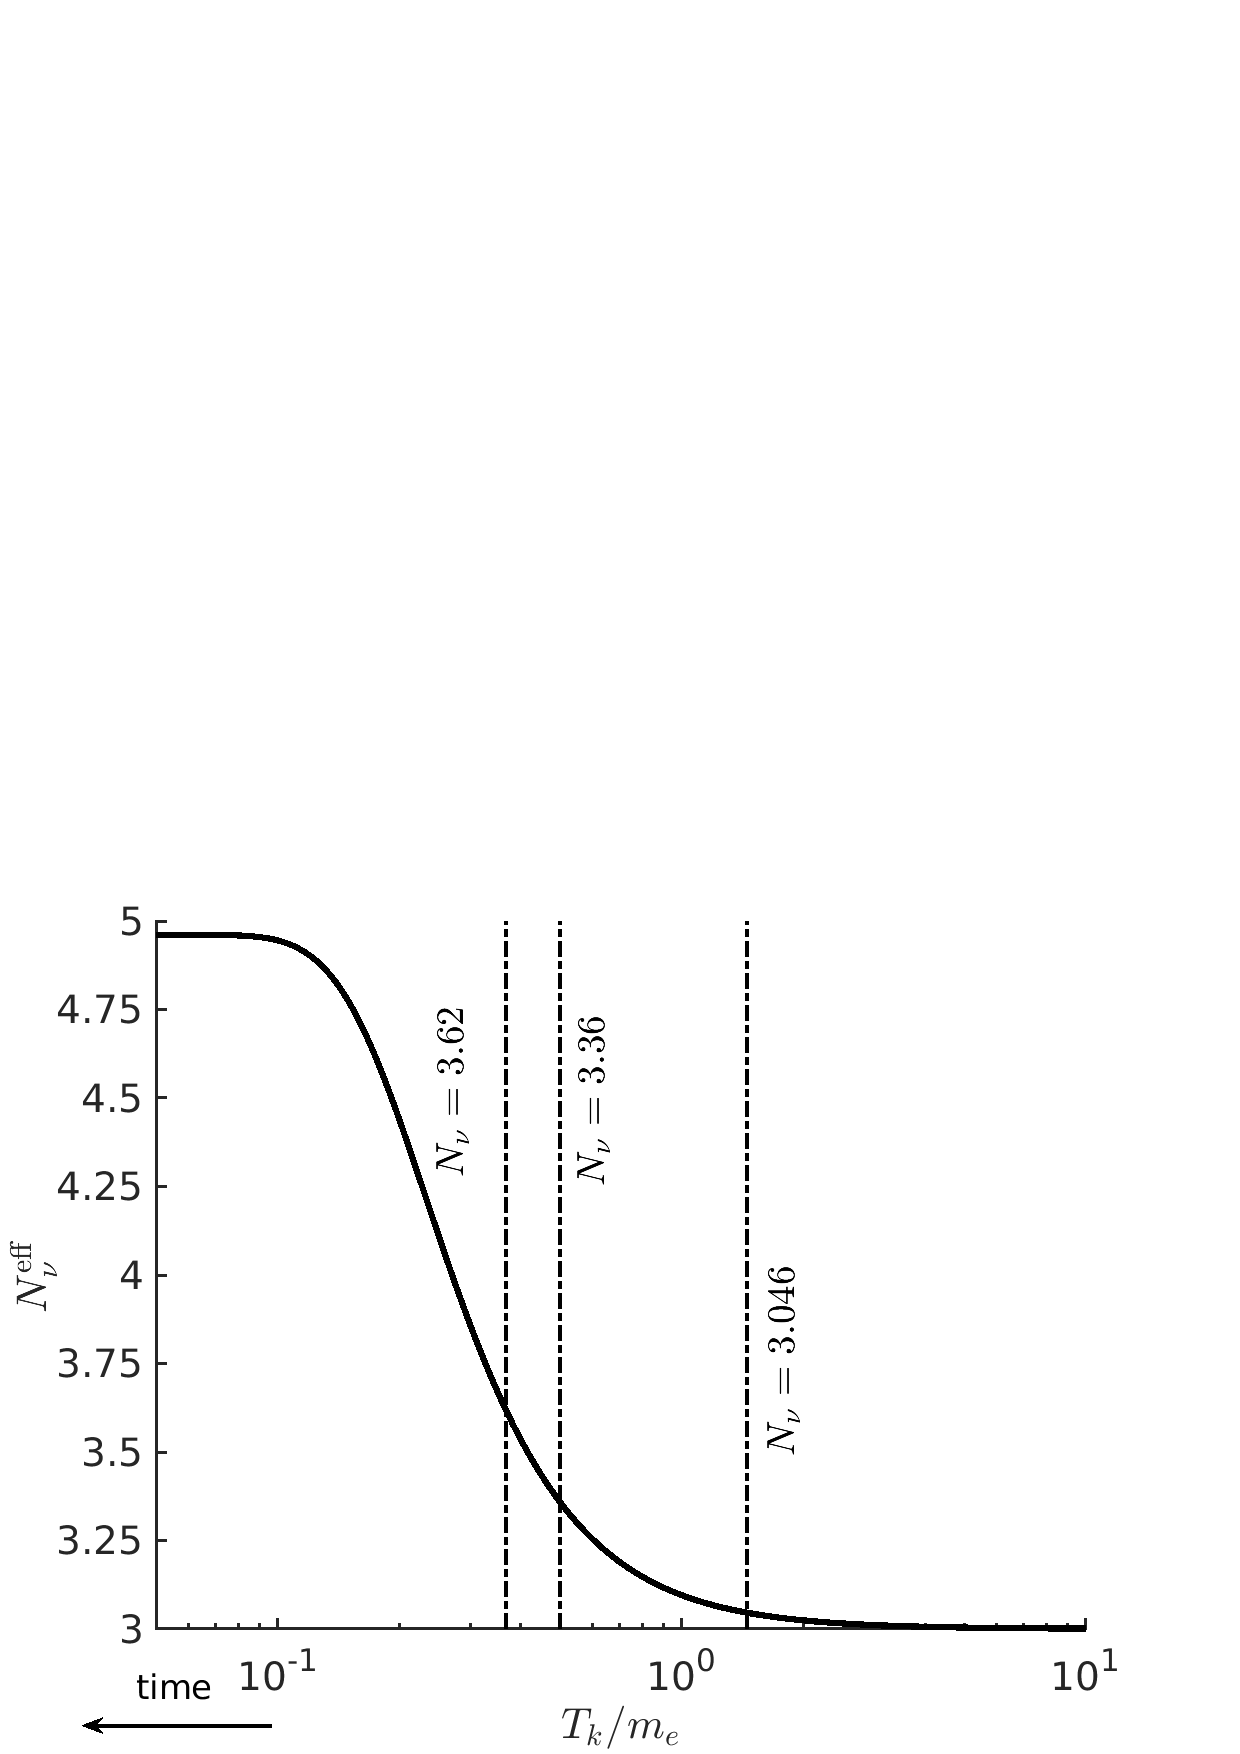
\includegraphics[width=0.51\linewidth]{plots/N_eff.pdf}\hspace{-0.95cm}
\includegraphics[width=0.50\linewidth]{plots/Upsilon_q.pdf}}
\caption{Dependence of the effective number of neutrinos (left hand frame) and neutrino fugacity\index{fugacity!neutrino} (right hand frame) on the neutrino kinetic freeze-out temperature. We also show the evolution of the deceleration parameter through the freeze-out period (right hand frame)}
\label{fig:Tk_dependence}
\end{figure}
%%%%%%%%%%%%%%%%%%%%%%%%%%%%%%%%%%%%%%%

In \rf{fig:Tk_dependence} we plot that dependence of $N^{\mathrm{eff}}_\nu$ and $\Upsilon$ on $T_k$ that is implied by these calculations. In particular, the fugacity evolves following the solid black curve in the bottom plot until it reaches the kinetic freeze-out temperature, at which point the neutrinos decouple and $\Upsilon$ remains constant thereafter, as shown in the dashed black curves for two sample values of $T_k$. 
 
The early Planck CMB\index{CMB} results~\cite{Planck:2013pxb} contain several fits based on different data sets which suggest that $N^{\mathrm{eff}}_\nu$ is in the range $3.30\pm 0.27$ to $3.62\pm0.25$ ($68\%$ confidence level). We note the more recent Planck CMB analysis~\cite{Planck:2018vyg} which chooses to sidestep these considerations, which in part gives rise to the Hubble-tension issues.

A numerical computation based on the Boltzmann equation with two body scattering~\cite{Mangano:2005cc} gives to $N_{\nu}^{\rm eff}=3.046$. These values are shown in the vertical lines in the left figure. The tension between the Planck results and theoretical reheating studies motivated some of our work.

%%%%%%%%%%%%%%%%%%%%%%%%%%%%%%%%%%%%%%%%%%%%%%%%%%%%%%%%%%%%%%%%%%%%
\para{Contribution to effective neutrino number from sub-eV mass sterile particles}
We  briefly explore  the effect on $N_\nu^{\text{eff}}$ by non-SM light weakly coupled particle species \cite{Birrell:2014cja}, referred to here as a sterile particles (SP)\index{sterile particles}. Independent of their source, once the SPs decouple from the particle inventory at a photon temperature of $T_{d,s}$, a difference in their temperature from that of photons will build up during subsequent photon reheating periods, similarly to earlier computations we presented.

Such hypothetical SPs would behave as `dark radiation'~\cite{Steigman:2013yua} rather than cold dark matter and would therefore impact $N_\nu^{\text{eff}}$ in a similar manner to neutrinos, though with a different freeze-out temperature not described by PP-SM.  The possibility that Goldstone bosons, one candidate for SPs, could be such dark radiation was identified in \cite{Weinberg:2013kea}. Another viable candidate for SPs are sterile neutrinos. In fact three sterile right-handed neutrinos could contribute with needed strength to the effective number of neutrinos\index{neutrino!effective number}, $N^{\text{eff}}_{\nu}$, if their freeze-out temperature is in the vicinity of the quark gluon plasma (QGP) phase transition~\cite{Anchordoqui:2011nh,Anchordoqui:2012qu}. 

If SPs originating in the QGP phase transition are interpreted as Goldstone bosons, this would imply that in the deconfined phase there is an additional hidden symmetry, weakly broken at hadronization. For example, if this symmetry were to be part of the baryon conservation riddle, then we can expect that these Goldstone bosons will couple to particles with baryon number, and possibly only in the domain where the vacuum is modified from its present day condition. These consideration motivate our study~\cite{Birrell:2014cja} of the contribution to 
$N^{\text{eff}}_{\nu}$ of boson or fermion degrees of freedom (DoF) that froze out near to the QGP phase transformation. 

We use the lattice-QCD derived QGP EoS from~\cite{Borsanyi:2013bia} to characterize the relation between $N^{\text{eff}}_{\nu}$ and the number of DoF that froze out at the time that the quark-gluon deconfined phase froze into hadrons near $T=150\MeV$. We work within the instantaneous freeze-out approximation, using the same reasoning that was applied to neutrinos, {\it i.e.\/}, we employ comoving entropy conservation\index{entropy!conservation} along with the facts that frozen-out particle species undergo temperature scaling with $1/a(t)$ and the remaining coupled particles undergo reheating at each $T\simeq m$ threshold, caused by a disappearing particle species transfer entropy into the remaining particles.

We denote by $S$ the conserved `comoving' entropy in a volume element $dV$, which scales with the factor $a(t)^3$. As we are no longer only considering just the neutrino freeze-out\index{neutrino!freeze-out}, here we employ the definition of the effective number of entropy DoF, $g_*^S$, given by
\begin{equation}
S=\frac{2\pi^2}{45}g^S_*T_\gamma^3 a^3\,.
\end{equation} 
For ideal fermion and boson gases, 
\begin{equation}
g_*^S=\!\!\!\!\sum_{i=\text{bosons}}\!\!\!\!g_i \left(\frac{T_i}{T_\gamma}\right)^3\!\!\!f_i^-+\frac{7}{8}\!\!\!\sum_{i=\text{fermions}}\!\!\!\! g_i \left(\frac{T_i}{T_\gamma}\right)^3\!\!\!f_i^+\,.
\end{equation}
The $g_i$ are degeneracies, $f_i^\pm$ are known functions, valued in $(0,1)$ (see \req{eq:entg002} for details), that turn off the various species as the temperature drops below their mass; compare to the analogous Eqs.\,(2.3) and (2.4) in~\cite{Blennow:2012de}. 

%%%%%%%%%%%%%%%%%%%%%%%%%%%%%%%%%%%%%%%
\begin{figure}
\centerline{\includegraphics[width=0.8\linewidth]{plots/gS_T_ratio.pdf}}
\caption{Left axis: Effective number of entropy-DoF, including lattice QCD effects applying~\cite{Borsanyi:2013bia} (solid line) and~\cite{HotQCD:2014kol} (circles), compared to the earlier results~\cite{Bazavov:2009zn} (triangles) used by~\cite{Anchordoqui:2011nh}, and the ideal gas model of~\cite{Coleman:2003hs} (dashed line) as functions of temperature $T$. Right axis: Photon to SP temperature ratio, $T_\gamma/T_s$, as a function of SP decoupling temperature (dash-dotted (blue) line). The vertical dotted lines at $T=142\MeV$ and $T=163\MeV$ delimit the QGP transformation region. \cccite{Birrell:2014cja}\label{fig:gS}}
 \end{figure}
%%%%%%%%%%%%%%%%%%%%%%%%%%%%%%%%%%%%%%%

Such a simple characterization does not hold in the vicinity of the QGP phase transformation where quark-hadron degrees of freedom are strongly coupled and the system must be studied using lattice QCD. A computation of $g_*^S$ that incorporates the lattice QCD results is shown in the solid line in \rf{fig:gS} (left axis). Specifically, we used the table of entropy density\index{entropy!density} values through the QGP phase transition presented by Borsanyi et al.~\cite{Borsanyi:2013bia}, while circles show recent results from Bazavov et al.~\cite{HotQCD:2014kol} correcting their earlier 2009 data\cite{Bazavov:2009zn} (triangles), also shown. This should be compared to the use of the ideal gas approximation (dashed) from~\cite{Coleman:2003hs} together with the fit in~\cite{Wantz:2009it} to interpolate though the QGP phase transition. The free gas approximation has a maximum error of $10\%$ in the QGP phase transition temperature range $T\simeq 150$\,MeV. The early 2009 lattice data, used in~\cite{Anchordoqui:2011nh} has a maximum error on the order of $25\%$, which leads to a non-negligible difference in the relation between freeze-out temperature and $N^{\text{eff}}_{\nu}$. 

Conservation of entropy leads to a temperature ratio at $T_\gamma<T_{d,s}$, shown in the dot-dashed line in Figure \ref{fig:gS} (right axis), given by
\begin{equation}\label{eq:TRatio}
R_s\equiv T_{s}/T_{\gamma}=\left(\frac{g_*^S(T_\gamma)}{g_*^S(T_{d,s})}\right)^{1/3}\,.
\end{equation}
Evolving the Universe through neutrino freeze-out\index{neutrino!freeze-out}, if $T_s$ and $T_\gamma$ are the light SP and photon temperatures, both after $e^\pm$ annihilation, and $g_s$ is the number of DoF of the SPs normalized to bosons (i.e., for fermions it includes an additional factor of $7/8$) then this leads to the following change in the effective number of neutrinos\index{neutrino!effective number} in excess of the SM value:
\begin{equation}\label{Neff1}
\delta N_{\text{eff}}\equiv N^{\text{eff}}_{\nu}-3.046=\frac{4g_s}{7}\left(\frac{T_s}{R_s T_{\gamma}}\right)^4\,,
\end{equation}
where $3.046$ is the SM neutrino contribution. Using \req{eq:TRatio} we can rewrite $\delta N_{\text{eff}}$ as
\begin{equation}\label{eq:deltaN}
\delta N_{\text{eff}}=\frac{4g_s}{7R_\nu^4}\left(\frac{g_*^S(T_{\gamma})}{g_*^S(T_{d,s})}\right)^{4/3}\,,
\end{equation}
where $T_{d,s}$ is the decoupling temperature of the SP and $T_{\gamma}$ is any photon temperature in the regime $T_{\gamma}\ll m_e$. The SM particles remaining (in relevant amounts) at such $T_{\gamma}$ are photons and SM neutrinos, the latter with temperature $R_\nu T_{\gamma}$, and so $g_*^S(T_{\gamma})=2+7/8\times 6\times 4/11$ and (see also Eq.(2.7) in~\cite{Blennow:2012de})
\begin{align}\label{eq:deltaN2}
\delta N_{\text{eff}}\approx&g_s\left(\frac{7.06}{g_*^S(T_{d,s})}\right)^{4/3}\,.
\end{align}

%%%%%%%%%%%%%%%%%%%%%%%%%%%%%%%%%%%%%%%
\begin{figure}
\centerline{\includegraphics[width=0.75\linewidth]{plots/Neff_Td_combined.pdf}}
\caption{Solid lines: Increase in $\delta N_{\text{eff}}$ due to the effect of $1,\dots,6$ light sterile boson DoF ($g_s=1,\dots,6$, bottom to top curves) as a function of freeze-out temperature $T_{d,s}$. Dashed lines: Increase in $\delta N_{\text{eff}}$ due to the effect of $1,\dots,6$ light sterile fermion DoF ($g_s=7/8\times 1,\dots,7/8\times 6$, bottom to top curves) as a function of freeze-out temperature $T_{d,s}$. The horizontal dotted lines correspond to $\delta N_{\text{eff}}+0.046=0.36,0.62,1$. The vertical dotted lines show the reported range of QGP transformation temperatures $T_c=142-163\MeV$. \cccite{Birrell:2014cja}\label{fig:NeffTdZoom}}
\end{figure}
%%%%%%%%%%%%%%%%%%%%%%%%%%%%%%%%%%%%

In Figure \ref{fig:NeffTdZoom} we plot $\delta N_{\text{eff}}$ as a function of $T_{d,s}$ for $1,\dots,6$ boson (solid lines) and fermion (dashed lines) DoF. For a low decoupling temperature $T_{d,s}<100$\,MeV; a single bose or fermi SP can help alleviate the observed tension in $N^{\text{eff}}_{\nu}$. Within the QGP hadronization\index{hadrons!hadronization} temperature range $T_c=142-163\MeV$ (marked by vertical dotted lines) we see that three boson degrees of freedom or four fermion degrees of freedom are the most likely cases to resolve the tension. If the SPs froze out in the QGP phase at $T_{d,s}\gg 163\MeV$ then a significantly larger number of SPs would be required. While such a scenario cannot be excluded, such a large number undiscovered weakly broken symmetries, or/and sterile neutrino-like particles, seems unlikely. Therefore we suggest that Figure \ref{fig:NeffTdZoom} pinpoints the QGP temperature range and below as the primary domain of interest for the freeze-out of a small to moderate number of hypothetical degrees of freedom, should an excess in $N_\nu^{\text{eff}}$ above the SM value be needed~\cite{Birrell:2014cja}.

\input{03a4ParametricStudies.tex}
\subsection{Neutrinos today}\label{ch:nu:today}
%%%%%%%%%%%%%%%%%%%%%%%%%%%%%%%%%%%%%%%%%%%%%%
We conclude our comprehensive exploration of neutrino freeze-out considering the distribution of free-streaming\index{relic neutrino!background} relic neutrinos in the present day, as seen from the reference frame of the moving Earth~\cite{Birrell:2014qna}. Such a study is prequel to the future experimental detection of the cosmic background neutrinos,  a challenge of great interest \cite{Stodolsky:1974aq,Cabibbo:1982bb,Shvartsman,Langacker:1982ih,Smith:1983jj,Tupper:1987sf,Ferreras:1995wf,Hagmann:1999kf,Duda:2001hd,Gelmini:2004hg,Ringwald:2009bg,Liao:2012wb,Hedman:2013hha}. With the  recently proposed PTOLEMY experiment, which aims to detect relic  electron-neutrino capture by tritium \cite{Betts:2013uya,PTOLEMY:2019hkd}, the characterization of the relic neutrino background is increasingly relevant.  Using our  characterization of the neutrino distribution after freeze-out and the subsequent free-streaming dynamics from  \rsec{sec:model:ind} and \cite{Birrell:2012gg}, we lay groundwork for a characterization of the present day relic neutrino spectrum, which we explore  from the  perspective of an observer moving relative to the neutrino background, including the dependence on neutrino mass\index{neutrino!mass} and effective number of neutrinos, $N_\nu^{\mathrm{eff}}$. Beyond consideration of the observable neutrino distributions, we evaluate the ${\cal O}(G_F^2)$ mechanical drag force acting on the moving observer. This section is adapted from the work in \cite{Birrell:2014qna}.

%%%%%%%%%%%%%%%%%
\para{Neutrino distribution in a moving frame}
The cosmic neutrino background (C$\nu$B)\index{C$\nu$B} and the cosmic microwave background (CMB)\index{CMB} were in equilibrium until decoupling (freeze-out) at $T_k\simeq {\cal O}{\rm (MeV)}$, hence one surmises that an observer would have the same relative velocity relative to the relic neutrino background  as with CMB. As a particular example in considering the spectrum, we present in more detail the case of an observer comoving with  Earth velocity $v_\oplus=300$\,km/s relative to the CMB,  modulated by orbital velocity ($\pm29.8$\,km/s).  We will write velocities in units of $c$, though our specific results will be presented in km/s.

In the cosmological setting, for $T<T_k$ the neutrino spectrum evolves according to the well known Fermi-Dirac-Einstein-Vlasov\index{Fermi!Einstein-Vlasov distribution} (FDEV) free-streaming\index{free-streaming} distribution~\cite{Langacker:1982ih,Choquet-Bruhat:2009xil,Wong:2011ip,Birrell:2012gg}.  By casting it in a relativistically invariant form we can then make a transformation to the rest frame of an observer moving with relative velocity $v_{\text{rel}}$ and obtain
\begin{align}\label{eq:neutrinoDistB}
f(p^\mu)=&\frac{1}{\Upsilon^{-1} e^{\sqrt{(p^\mu U_\mu)^2-m_\nu^2}/T_\nu}+1}\,.
\end{align}
The 4-vector characterizing the rest frame of the neutrino FDEV distribution is
\begin{equation}
U^\mu=(\gamma,0,0,v_{\text{rel}}\gamma)\,,\hspace{2mm} \gamma={1}/{\sqrt{1-v_{\text{rel}}^2}}\,,
\end{equation} 
where we have chosen coordinates so that the relative motion is in the $z$-direction. 

The neutrino effective temperature $T_\nu(t)= T_k\,(a(t_k)/a(t))$ is the scale-shifted freeze-out temperature $T_k$. Here $a(t)$ is the cosmological scale factor where $\dot a(t)/a(t)\equiv H$ is the observable Hubble parameter\index{Hubble!parameter}. $\Upsilon$ is the fugacity\index{fugacity} factor, here describing the underpopulation of neutrino phase space that was frozen into the neutrino FDEV distribution in the process of decoupling from the $e^\pm,\gamma$-QED background  plasma.

There are several available bounds on neutrino masses\index{neutrino!mass}. Neutrino energy and pressure components are important before photon freeze-out and thus $m_\nu$ impacts Universe dynamics. The analysis of CMB data alone leads to $\sum_i m_\nu^i<0.66$eV ($i=e,\mu,\tau$) and including Baryon Acoustic Oscillation (BAO) gives $\sum m_\nu<0.23$eV~\cite{Planck:2013pxb}.  {\small PLANCK CMB} with lensing observations~\cite{Battye:2013xqa} lead to  $\sum m_{\nu}=0.32\pm0.081$ eV. Upper bounds have been placed on the electron neutrino mass in direct laboratory measurements  $m_{\bar\nu_e}<2.05$eV~\cite{Troitsk:2011cvm}.   In the subsequent analysis we will focus on the neutrino mass range $0.05$eV to $2$eV in order to show that direct measurement sensitivity allows the exploration of a wide mass range. 

 The relations in \req{modindeq1}\,-\,\req{modindeq3}, see also~\cite{Birrell:2012gg}, determine $T_\nu/T_\gamma$ and  $\Upsilon$ in terms of the measured  value of  $N_\nu^{\mathrm{eff}}$ under the assumption of a strictly SM-particle inventory.  In the following we treat $N_\nu^{\mathrm{eff}}$  as a variable model parameter and use the above mentioned relations to characterize our results in terms of $N_\nu^{\mathrm{eff}}$.

%%%%%%%%%%%%%%%%%%%%%%%
\para{Velocity, energy, and wavelength distributions}
Using \req{eq:neutrinoDistB}, the normalized FDEV velocity distribution for an observer in relative motion has the form
\begin{align} \label{fvdistrib}
&f_v=\frac{g_\nu}{n_\nu 4\pi^2}\!\!\!\int_0^\pi \!\!\!\!\frac{ p^2dp/dv\sin(\phi) d\phi}{\Upsilon^{-1}e^{\sqrt{( E-v_{\text{rel}} p \cos(\phi))^2\gamma^2-m_\nu^2}/T_\nu}+1}\,,\notag\\
&p(v)=\frac{m_\nu v}{\sqrt{1-v^2}}\,,\qquad \frac{dp}{dv}=\frac{m_\nu}{(1-v^2)^{3/2}}\,.
\end{align}
The normalization $n_\nu$ depends on $N_\nu^{\mathrm{eff}}$ but not on $m_\nu$ since decoupling occurred at $T_k\gg m_\nu$. For each neutrino flavor (all flavors are equilibrated by oscillations) we have, per neutrino or antineutrino and at nonrelativistic relative velocity,
\begin{equation}\label{nnu}
n_\nu=[-0.3517(\delta N_\nu^{\mathrm{eff}})^2+6.717\delta N_\nu^{\mathrm{eff}}+56.06]\,{\rm cm}^{-3}
\end{equation}
($\delta N_\nu^{\mathrm{eff}}\equiv N_\nu^{\mathrm{eff}}-3$), compare to Eq.(55) in Ref.~\cite{Birrell:2012gg}.

We show $f_v$ in Figure \ref{fig:RelvDist300} for several values of the neutrino mass\index{neutrino!mass}, $v_{\text{rel}}=300$ km/s, and $N_\nu^{\mathrm{eff}}=3.046$ (solid lines) and $N_\nu^{\mathrm{eff}}=3.62$ (dashed lines). As expected, the lighter the neutrino, the more $f_v$  is weighted towards higher velocities with the velocity becoming visibly peaked about $v_{\text{rel}}$ for $m_\nu=2$ eV. 
%%%%%%%%%%%%%%%%%%%%%%%%%%%%%%%%%%%%%%%

%%%%%%%%%%%%%%%%%%%%%%%%%%%%%%%%%%%%%%%
\begin{figure}
\centerline{\includegraphics[width=0.9\linewidth]{plots/rel_v_dist_300.pdf}}
\caption{Normalized neutrino FDEV velocity distribution in the Earth frame. We show the distribution for $N_\nu^{\mathrm{eff}}=3.046$ (solid lines) and $N_\nu^{\mathrm{eff}}=3.62$ (dashed lines). \cccite{Birrell:2014qna}}
\label{fig:RelvDist300}
 \end{figure}
%%%%%%%%%%%%%%%%%%%%%%%%%%%%%%%%%%%%%%%

A similar procedure produces the normalized FDEV energy distribution $f_E$.  In \req{fvdistrib} we replace $dp/dv\to dp/dE$ where it is understood that 
\begin{equation}
p(E)=\sqrt{E^2-m_\nu^2},\qquad \frac{dp}{dE}=\frac{E}{p}.
\end{equation}
We show $f_E$ in Figure \ref{fig:EDist300}  for several values of the neutrino mass, $v_{\text{rel}}=300$ km/s, and $N_\nu^{\mathrm{eff}}=3.046$ (solid lines) and $N_\nu^{\mathrm{eff}}=3.62$ (dashed lines). The width of the FDEV energy distribution is on the micro-eV scale and the kinetic energy $T=E-m_\nu$ is peaked about $T=\frac{1}{2}m_\nu v_{\text{rel}}^2$, implying that the relative velocity between the Earth and the CMB\index{CMB} is the dominant factor for $m_\nu>0.1$ eV.

%%%%%%%%%%%%%%%%%%%%%%%%%%%%%%%%%%%%%%%
\begin{figure}
\centerline{\includegraphics[width=0.9\linewidth]{plots/E_dist_300.pdf}}
\caption{Neutrino FDEV energy distribution in the Earth frame. We show the distribution for $N_\nu=3.046$ (solid lines) and $N_\nu=3.62$ (dashed lines). \cccite{Birrell:2014qna}}
\label{fig:EDist300}
 \end{figure}
%%%%%%%%%%%%%%%%%%%%%%%%%%%%%%%%%%%%%%%

By multiplying $f_E$ by the neutrino velocity and number density for a single neutrino flavor (without anti-neutrinos) we obtain the particle flux density,
 \begin{equation}
 \frac{dJ}{dE}\equiv\frac{dn}{dAdtdE}\,,
\end{equation} 
shown in Figure \ref{fig:fluxDist}. We show the result for $N_\nu^{\mathrm{eff}}=3.046$ (solid lines) and $N_\nu^{\mathrm{eff}}=3.62$ (dashed lines). The flux is normalized in these cases to a local density $56.36$~cm${}^{-3}$ and $60.10$~cm${}^{-3}$, respectively. 

The precise neutrino flux in the Earth frame is significant for efforts to detect relic neutrinos, such as the PTOLEMY experiment~\cite{Betts:2013uya}. The energy dependence of the flux shows a large sensitivity to the mass. However, the maximal fluxes do not vary significantly with $m$. In fact the maximum values are independent of $m$ when $v_{\text{rel}}=0$, as follows from the fact that $v=p/E=dE/dp$.  In the Earth frame, where $0<v_\oplus\ll c$, this translates into only a small variation in the maximal flux.

%%%%%%%%%%%%%%%%%%%%%%%%%%%%%%%%%%%%%%%
\begin{figure}
\centerline{\includegraphics[width=0.9\linewidth]{plots/flux_dist.pdf}}
\caption{Neutrino flux density in the Earth frame. We show the result for $N_\nu^{\mathrm{eff}}=3.046$ (solid lines) and $N_\nu^{\mathrm{eff}}=3.62$ (dashed lines) for an observer moving with $v_\oplus=300$\,km/s. \cccite{Birrell:2014qna}}
\label{fig:fluxDist}
 \end{figure}
%%%%%%%%%%%%%%%%%%%%%%%%%%%%%%%%%%%%%%%

Using $\lambda=2\pi/p$, we find  the normalized FDEV de Broglie wavelength distribution
\begin{equation}
%\frac{dn}{d\lambda}
f_\lambda=\frac{ 2\pi g_\nu}{n_\nu\lambda^4}\!\!\int_0^\pi\!\!\! \!\frac{\sin(\phi) d\phi}{\Upsilon^{-1}e^{\sqrt{( E-v_{\text{rel}} p \cos(\phi))^2\gamma^2-m_\nu^2}/T_\nu}\!\!+\!1}\,,
\end{equation}
shown in Figure \ref{fig:deBrogle300} for $v_{\text{rel}}=300$ km/s and for several values $m_\nu$ comparing  $N_\nu^{\mathrm{eff}}=3.046$ with $N_\nu^{\mathrm{eff}}=3.62$. 

%%%%%%%%%%%%%%%%%%%%%%%%%%%%%%%%%%%%%%%
\begin{figure} 
\begin{minipage}{\textwidth}
\makebox[0.5\linewidth]%
{\includegraphics[height=5.4cm]{plots/deBrogle_300.pdf}}
\makebox[0.5\linewidth]%
{\includegraphics[height=5.4cm]{plots/f_ratio.pdf}}
\end{minipage}
\caption{Neutrino  FDEV de Broglie wavelength  distribution in the Earth frame. We show in left panel the distribution for $N_\nu^{\mathrm{eff}}=3.046$ (solid lines) and $N_\nu^{\mathrm{eff}}=3.62$ (dashed lines) and in right panel their ratio. \cccite{Birrell:2014qna}.  }\label{fig:deBrogle300}
 \end{figure}
%%%%%%%%%%%%%%%%%%%%%%%%%%%%%%%%%%%%%%%%%%%%%%%%%

%%%%%%%%%%%%%%%%%%%%%%%%%%%%%%%
\para{Drag force}
Given the neutrino distribution, we evaluate the drag force due to the anisotropy of the neutrino distribution in the rest frame of the moving object for $N_\nu^{\mathrm{eff}}=3.046$. The relic neutrinos will undergo potential scattering with the scale of the potential strength being
\begin{equation}\label{V0}
V_0=CG_F\rho_{N_c},\hspace{2mm} \rho_N\equiv N_c/R^3
\end{equation}
where $R$ is the linear size of the detector.  

When the detector size is smaller than the quantum de Broglie wavelength of the neutrino, all scattering centers are added coherently to for the target effective `charge' $N_c$.  $\rho_{N_c}$ is the charge density, and C=O(1) and is depending on material composition of the object. Such considerations are of interest both for scattering from terrestrial detectors, as well as for ultra-dense objects of neutron star matter density, e.g.   strangelet  CUDOS~\cite{Rafelski:2011bby} - recall that such nuclear matter fragments with $R<\lambda$  despite their small size would have a mass rivaling that of large meteors. We find $V_0\simeq 10^{-13}$ eV for normal matter densities, but for nuclear target density a potential well with $V_0\simeq {\cal O}(10 {\rm eV})$.  

We consider relic neutrino potential scattering to obtain the average momentum transfer to the target and hence the drag force. The particle flux per unit volume in momentum space is
\begin{equation}\label{dnQuantum}
\frac{dn}{dtd Ad^3{\bf p}}({\bf p})=\frac{2}{(2\pi)^3}f({\bf p})p/m_\nu\,,\hspace{2mm} p\equiv |{\bf p}|\,,
\end{equation}
where the factor of two comes from combining neutrinos and anti-neutrinos of a given flavor. 

Our use of nonrelativistic velocity is justified by  \rf{fig:RelvDist300}.  The recoil change in detector momentum per unit time is  
\begin{align}
\frac{d{\bf p}}{dt}=& \int  {\bf q}A \frac{dn}{dtdAd^3p}({\bf p})d^3p\,,\\
{\bf q}A\equiv &\int ({\bf p}-{\bf p_f})\frac{d\sigma}{ d\Omega}({\bf p_f},{\bf p})d\Omega\,.
\end{align}
Here ${\bf p}$ and ${\bf p}_f$, the incoming and outgoing momenta respectively, have the same magnitude. $qA$ is the momentum transfer times area, averaged over outgoing momenta, and $d\Omega$ is the solid angle for to ${\bf p}_f$.  

For a spherically symmetric potential, the differential cross section depends only on the incoming energy and the angle $\phi$ between ${\bf p}$ and ${\bf p_f}$.  Therefore, for each ${\bf p}$ the integral over $d\Omega$ of the components orthogonal to ${\bf p}$ is zero by symmetry.  This implies
\begin{align}
{\bf q}A\equiv &2\pi{\bf p}\int(1-\cos(\phi))\frac{d\sigma}{ d\Omega}(p,\phi)\sin(\phi)d\phi\,.
\end{align}
The only angular dependence in the neutrino distribution is in ${\bf p}\cdot {\bf\hat z}$ and therefore the components of the force orthogonal to ${\bf \hat z}$ integrate to zero, giving
\begin{align}\label{drag}
\frac{d{\bf p}}{dt}=&\frac{{\bf\hat z}}{\pi m_\nu } \int p^4g(p) f(p,\tilde\phi) \cos(\tilde\phi) \sin(\tilde\phi) dpd\tilde\phi\,,\\
g(p)\equiv& \int_0^\pi(1-\cos(\phi))\frac{d\sigma}{ d\Omega}(p,\phi)\sin(\phi)d\phi\,.\label{geq}
\end{align}

For the case of normal density matter, the Born approximation is valid due to the weakness of the potential compared to the neutrino energy seen in Figure \ref{fig:EDist300}. To obtain an order of magnitude estimate, we take a Gaussian potential \begin{equation}
V(r)=V_0e^{-r^2/R^2}\,,
\end{equation}
for which the differential cross section in the Born approximation can be analytically evaluated
\begin{align}
&\frac{d\sigma}{ d\Omega}(p,\phi)=\frac{\pi m_\nu^2V_0^2R^6}{4}e^{-q^2R^2/2}\,,\notag\\
&q=|{\bf p}-{\bf p}_f|=2p\sin(\phi/2)\,.
\end{align}

The integral over $\phi$ in \req{geq} can also be done analytically, giving
\begin{align}
g(p)=&\pi m_\nu^2V_0^2R^6\frac{1-(2R^2p^2+1)e^{-2R^2p^2}}{4R^4p^4}\,.
\end{align}
 In the long and short wavelength limit we have 
\begin{align}
\label{longWaveDrag}
&g(p)\simeq\frac{\pi}{2} m_\nu^2V_0^2R^6\,,\quad pR\ll 1\,,\\
&F_L\simeq \frac{m_\nu V_0^2R^6}{2} \int p^4 f(p,\tilde\phi) \cos(\tilde\phi) \sin(\tilde\phi) dpd\tilde\phi\,,\notag\\
\label{shortWaveDrag}
&g(p)\simeq\frac{\pi m_\nu^2V_0^2R^2}{4p^4}\,, 
\quad pR\gg 1\,,\\
&F_S\simeq \frac{ m_\nu V_0^2R^2}{4} \int f(p,\tilde\phi) \cos(\tilde\phi) \sin(\tilde\phi) dpd\tilde\phi\notag\,.
\end{align}
 We also note that in the short wavelength limit, our coherent scattering treatment is only applicable to properly prepared structured targets \cite{Liao:2012wb}.

Inserting \req{V0} we see that this force is $O(G_F^2)$, see also \cite{Shvartsman,Smith:1983jj,Gelmini:2004hg}, as compared to the $O(G_F)$ effects debated in  \cite{Opher:1974drq,Lewis:1979mu,Opher2,Cabibbo:1982bb,Langacker:1982ih,Smith:1983jj,Ferreras:1995wf}. In long wavelength limit the size $R$ cancels, in favor of $N_c^2$ which explicitly shows that scattering is on the square of the charges of the target. 

This results in an enhancement of the force by a factor of $N_c$ over the incoherent scattering case, due to $V_0^2$ scaling with $N_c^2$. This effect exactly parallels the proposed detection of supernovae MeV energy scale neutrinos by means of collisions with the entire atomic nucleus~\cite{Divari:2012zz}.  

Fits to the integrals in the above force formulas \req{longWaveDrag} and \req{shortWaveDrag} can be obtained in the region $0.005 \text{eV}\leq m_\nu\leq 0.25\text{eV}$, $v_\text{rel}\leq 300$km/s, yielding
\begin{align}\label{FL}
F_L\!=&8\,10^{-34}{\rm N}\!\left(\!\frac{m_\nu}{0.1 \text{eV}}\!\right)^{\!\!2}\!\! \left(\!\frac{V_0}{1\text{peV}}\!\right)^{\!\!2}\!\!\left(\!\frac{R}{1\text{mm}}\!\right)^{\!\! 6} \!\!\frac{v_{\text{rel}}}{v_\oplus},\\[0.2cm]
F_S=&2\, 10^{-35}{\rm N}\!\left(\!\frac{m_\nu}{0.1\text{eV}}\!\right)^{\!\!2}\! \left(\!\frac{V_0}{1\text{peV}}\!\right)^{\!\!2}\!\!\left(\!\frac{R}{1\text{mm}}\!\right)^{\!\!2}\times\notag \\
&\hspace*{1.5cm}\times\frac{v_{\text{rel}}}{v_\oplus}\!\left(\!1\!-\!0.2\frac{m_\nu}{0.1\text{eV}}\frac{v_{\text{rel}}}{v_\oplus}\right).
\end{align}
We emphasize that they are not valid in the limit as $m_\nu\rightarrow 0$. Considering that the current frontier of precision force measurements at the level of individual ions is on the order of $10^{-24}$N \cite{Biercuk}, the ${\cal O}(G_F^2)$ force on a coherent mm-sized terrestrial detector is negligible, despite the factor of $N_c$ enhancement. 

We now consider scattering from nuclear matter density $\rho_N\simeq 3 \, 10^{8}{\rm kg/mm}^3$ objects where $V_0={\cal O}(10\text{eV})$ is effectively infinite compared to the neutrino energy unless the object velocity relative to the neutrino background is ultra-relativistic.  Therefore we are in the hard `ball' scattering limit. As with the analysis for normal matter density, we will investigate both the long and short wavelength limits. 

In the long wavelength limit, only the S-wave contributes to hard sphere scattering and $d\sigma/d\Omega=R^2$, independent of angle. Using \req{drag} and a similar fit to \req{FL} gives
\begin{align}\label{FLHard}
F_L=&\frac{2\pi^2R^2}{\pi m_\nu} \int p^4 f(p,\tilde\phi) \cos(\tilde\phi) \sin(\tilde\phi) dpd\tilde\phi\notag\\
\simeq &\, 2\, 10^{-22}{\rm N}\left(\frac{R}{1\text{mm}}\right)^2\frac{v_{\text{rel}}}{v_\oplus}\,.
\end{align}
In particular the force is independent of $m_\nu$.  We also note that at high velocity, \req{FLHard}  underestimates the drag force. The resulting acceleration is
\begin{equation}
a=4\, 10^{-31}\frac{m}{s^2}\frac{v_{\text{rel}} }{v_\oplus}\! \left(\frac{R}{1\text{mm}}\right)^{-1}\!\!\left(\frac{\rho}{\rho_N}\right)^{-1}\,.\!\!
\end{equation}

The Newtonian drag time constant, $v_{\rm rel}/a$, is
\begin{equation}
\tau= 2\,10^{28}\text{yr}\frac{R}{1\text{mm}}\,\frac{\rho}{\rho_N}\,,
\end{equation}
which suggests that the compact object produced early on in stellar evolution remain largely unaltered.

The last case to consider is the short wavelength hard sphere scattering limit.  This limit is classical and so we no longer treat it as quantum mechanical potential scattering, but rather as elastic scattering of point particle neutrinos from a hard sphere of radius $R$.  

For a single scattering event where the component of the momentum normal to the sphere is ${\bf p}^\perp=({\bf p}\cdot \hat {\bf r}) \hat {\bf r}$, the change in particle momentum is  $\Delta {\bf p}=-2{\bf p}^\perp$. The particle flux per unit volume in momentum space at a point ${\bf r}$ on a radius $R$ sphere $S_R^2$ and inward pointing momentum ${\bf p}$ (i.e. ${\bf p}\cdot \hat{\bf  r}<0$) is
\begin{equation}\label{dnClassical}
\frac{dn}{dtd Ad^3{\bf p}}({\bf x},{\bf p})=\frac{2}{(2\pi)^3}f({\bf p})|{\bf v}\cdot \hat{\bf r}|\,,
\end{equation}
where the factor of two comes from combining neutrinos and anti-neutrinos of a given flavor.  

Note that for point particles the flux is proportional to the normal component of the velocity, as opposed to wave scattering where it is proportional to the magnitude of the velocity, seen in \req{dnQuantum}.

Using \req{dnClassical}, the recoil change in momentum per unit time is  
\begin{equation}
\frac{d{\bf p}}{dt}= -\frac{2}{(2\pi)^3}\int_{{\bf p}\cdot \hat{\bf r}<0} \!\!\!\!\!\!\Delta {\bf p}  f({\bf p}) \frac{1}{m_\nu}|{\bf p}\cdot \hat{\bf r}| d^3{\bf p}R^2d\Omega\,.
\end{equation}
The only angular dependence in $f$ is through ${\bf p}\cdot \hat {\bf z}$ so by symmetry, the ${\bf \hat x}$ and ${\bf \hat y}$ components integrate to $0$.  Therefore we have
\begin{equation}
\frac{d{\bf p}}{dt}=-\frac{R^2\hat{\bf z}}{2\pi^3m_\nu}\int_{{\bf p}\cdot \hat{\bf r}<0}\!\!\!   f({\bf p}) ({\bf p}\cdot \hat{\bf r})^2 \hat {\bf r}\cdot\hat{\bf z}\, d^3{\bf p}d\Omega\,.  
\end{equation}

We perform this integration in spherical coordinates for ${\bf r}$ and in the spherical coordinate vector field basis for ${\bf p}=p_r\hat{\bf r} +p_\theta\hat{\bf r}_\theta+p_\phi\hat{\bf r}_\phi,\hspace{2mm} p_r<0$, where we recall
\begin{align}
&\hat{\bf r}=\cos  \theta \sin \phi \, \hat{\bf x}+\sin \theta \sin \phi \hat{\bf y}+\cos  \phi\,\hat{\bf z}\notag\,,\\
&\hat{\bf r}_\theta=-\sin \theta \hat{\bf x}+\cos \theta \hat{\bf y}\,,\\
&\hat{\bf r}_\phi=\cos \theta \cos \phi\,\hat{\bf x}+\sin \theta \cos \phi \,\hat{\bf y}-\sin \phi \, \hat{\bf z}\notag\,.
\end{align}
Therefore the force per unit surface area is
\begin{align}
\frac{1}{A}\frac{d{\bf p}}{dt}=&-\frac{1}{4\pi^3 m_\nu}\int_0^\pi\!\!\int_{p_r<0}\!\!\!\!\!\!\!\! f({\bf p}) p_r^2  d^3{\bf p}\cos \phi \sin \phi  d\phi\hat{\bf z}\,,\notag\\
f({\bf}p)=&\frac{1}{  \Upsilon^{-1}e^{\sqrt{( E-V_\oplus {\bf p}\cdot \hat {\bf z})^2\gamma^2-m_\nu^2}/T_\nu}+1 }\,,\\
          &{\bf p}\cdot\hat{\bf z}=p_r\cos \phi-p_\phi\sin\phi \,.\notag
\end{align}

We obtain an approximation over the range $v_{\text{rel}}\leq v_\oplus ;\ 0.05\text{eV}\leq m_\nu\leq 0.25\text{eV}$ given by
\begin{align}
&F_S =  4\,10^{-23} \text{N}\left(\frac{R}{1{\rm mm}}\right)^2\frac{v_{\text{rel}}}{ v_\oplus}\,.
\end{align}
This is a result similar to the long wavelength hard sphere limit \req{FLHard}, but the fact that it is only applicable to objects larger than the neutrino wavelength means that the acceleration it generates is negligible on the timescale of the Universe.

%%%%%%%%%%%%%%%%%%%%%%%%%%%%%%%%%%
\para{Prospects for detecting relic neutrinos}
In this section we characterized the relic cosmic neutrinos and their velocity, energy, and de Broglie wavelength distributions in a frame of reference moving relative to the neutrino background. We have shown explicitly the mass $m_\nu$ dependence and the dependence on neutrino reheating expressed by $N_\nu^{\mathrm{eff}}$, choosing a range within the experimental constraints. This is a necessary input for the measurement of $N_\nu^{\mathrm{eff}}$ and neutrino mass by future detection efforts.  

Finally, we have discussed in detail the $O(G_F^2)$ mechanical drag force  originating in the dipole anisotropy induced by motion relative to the neutrino background.  Despite enhancement with the total target charge found within the massive neutrino wavelength, the magnitude of the force is found to be well below the reach of current  precision force measurements.

Our results are derived under the assumption that $N_\nu^{\mathrm{eff}}$ is due entirely to SM neutrinos, with no contribution from new particle species. In principle future relic neutrino detectors, such as PTOLEMY~\cite{Betts:2013uya,PTOLEMY:2019hkd}, will be able to distinguish between these alternatives since the effect of $N_\nu^{\mathrm{eff}}$ as presented here is to increase neutrino flux~\cite{Birrell:2012gg}, see \req{nnu}. However, to this end one must gain precise control over the enhancement of neutrino galactic relic density due to  gravitational effects~\cite{Ringwald:2004np} as well as the annual modulation~\cite{Safdi:2014rza}. 

%%%%%%%%%%%%%%%%%
\section{Plasma physics methods: Electromagnetic fields,  BBN}\label{part4}
\subsection{Plasma response to electromagnetic fields}
\label{chap:PlasmaSF}
The interaction of electromagnetic fields within relativistic plasma is of interest in wide are of cosmology, astrophysics, and laboratory environments involving  intense laser interactions with matter, and  relativistic heavy-ion collisions forming the new phase of matter, quark-gluon plasma, in relativistic heavy-ion collisions, which discovery allows to probe in the laboratory some aspects of the primordial Universe as we have discussed before, see \rsec{chap:QCD}. Several methods have been introduced to study the linear response of a collisionless ultrarelativistic QGP following the seminal work by~\cite{Weldon:1982aq} by using semiclassical transport theory based on the Boltzmann equation~\cite{Mrowczynski:1987jr,Mrowczynski:1989np,Blaizot:1993zk,Kelly:1994ig,Kelly:1994dh}. However, applications of this formalism are restricted to dilute plasmas where collisions can be neglected~\cite{Blaizot:2001nr}. 

Here, we will study semi-classical transport using the Vlasov-Boltzmann equation\index{Vlasov-Boltzmann equation} with momentum-averaged quantum collisions between particles, a topic discussed in numerous other works, such as \cite{DeGroot:1980dk,Cercignani:2002bk,Hakim:2011bk,Carrington:2003je,Schenke:2006xu}.
Previously, the effects of collisions within the plasma were mainly studied to derive transport coefficients, such as the electrical conductivity, of interest to the study of plasma response to long-wavelength perturbations~\cite{Mrowczynski:1988xu,Heiselberg:1993cr,Ahonen:1996nq,Baym:1997gq,Ahonen:1998iz}. In quantum field theory, transport coefficients have also been calculated using effective propagators that re-sum thermal modifications to avoid infrared divergences~\cite{Heiselberg:1994ms,Arnold:2002zm,Arnold:2003zc}.

The theoretical description of relativistic interacting  plasma is based on transport theory, i.e., the relativistic form of Liouville's equation. The one-particle phases space distribution function $f(x,p)$ undergoes Liouville flow,
\begin{align}
    \frac{d f(x,p)}{d\tau} = \{H(x,p), f(x,p)\} = 0\,,
\end{align}
where $p$ is the canonical four-momentum, and $x$ is the canonical position. The collision term $C[f]$ represents elastic/inelastic interactions and gives deviations away from Liouville's theorem
\begin{align}\label{eq:LpC}
    \frac{d f(x,p)}{d\tau} = C[f]\,,
\end{align}
or equivalently, entropy generation. The collision term is necessary to describe systems where the mean free path of plasma constituents is less than or equal to the characteristic length scale of the plasma or when the mean free time $\tau$ is smaller than the characteristic oscillation time of the plasma. This pertains to systems with high density, low temperature, or strongly coupled systems.

The Boltzmann-Einstein equation, see  \rsec{sec:BoltzmannEinstein}, with a realistic collision operator, i.e., modeling scattering among neutrinos and $e^\pm$, was used in Section \ref{ch:param:studies} to  study the cosmological neutrino freeze-out. However, in many cases a detailed treatment of the microscopic collision term \req{eq:collisionMicro} is computationally prohibitive.  In this section our focus is on the interaction of electromagnetic fields within relativistic plasmas and so in place of the microscopic collision term we employ the relaxation-time approximation (RTA) technique, as proposed by~\cite{Anderson:1974nyl}. 

RTA is a commonly made simplification to the Boltzmann equation, reducing it from an integrodifferential equation to a differential equation. The relativistic form of this collision term takes the form
\begin{equation}\label{eq:lincoll}
C[f] = (p^\mu u_\mu) \kappa [ f_\mathrm{eq}(p) - f(x,p) ] \,,
\end{equation}
where $\kappa=1/\tau$ is the relaxation rate, $f(x,p)$ is the phase space distribution of charged particles in the plasma, $f_\mathrm{eq}(p)$ is their equilibrium distribution, and $u_\mu$ is the four-velocity of the plasma rest frame.

The RTA collision term assumes the nonequilibrium distribution $f$ returns to the equilibrium distribution in some characteristic time $\tau$, which is evident when writing \req{eq:LpC} in the form
\begin{equation}
    \frac{d f(x,p)}{dt} = \frac{f_\mathrm{eq}(p) - f(x,p) }{\tau}\,.
\end{equation}
The relaxation time $\tau$ can be computed using the schematic relaxation time approximation where an average relaxation time is introduced~\cite{Mrowczynski:1988xu,Satow:2014lia} or by calculating the momentum-dependent relaxation rate $\kappa(p)$ with the input of perturbative matrix elements~\cite{Ahonen:1996nq}. We use the average relaxation time approximation with momentum averaged $\kappa$ to make all calculations analytically tractable.

The well-known disadvantage of the RTA is that it forces all quantities, even conserved ones, to return to their equilibrium value at a rate $\tau$. This can cause the dynamics derived from this collision term to violate current and energy-momentum conservation. The violation of energy conservation is similar to introducing frictional damping into one particle Newtonian dynamics where energy is lost to the environment.

Correcting for current and energy-momentum conservation is possible by adding terms that ensure that conserved quantities are unaffected~\cite{Bhatnagar:1954zz,Greene1973,Rocha:2021zcw,Singha:2023eia}. It is worth noting that this breaking of conservation law does not always affect the physical behavior of the plasma. For instance, the behavior of transverse waves in an infinite homogeneous plasma is unaffected by the addition of current conservation~\cite{Formanek:2021blc}.

We generalize the BGK modification of the linearized collision term to relativistic plasmas using the Anderson-Witting form Eq.\,(\ref{eq:lincoll}), ensuring current conservation \req{eq:collision} but not energy-momentum conservation. In \cite{Formanek:2021blc} we have shown that the resulting linear response functions satisfy current conservation and gauge invariance constraints. 

The preceding sections will discuss obtaining exact solutions for the covariant polarization tensor in linear response limit via Fourier transform with the BGK collision term \req{eq:collision}. We will present the plasma's electromagnetic properties by using the polarization tensor to derive the electromagnetic fields.

%%%%%%%%%%%%%%%%%%%%%%%%%%%%%%%%%%% 
\para{Covariant kinetic theory}
%\label{sec:CKT}
A full microscopic picture of plasma kinematics, useful in numerical simulations, is often more involved than what is required to understand changes in the macroscopic quantities of plasmas. A conventional simplification to the microscopic picture is to average over the discrete states to yield a distribution function $f(x,\boldsymbol{p})$, which describes the probability of finding some number of particles $dN$ in a small range of position $d\mathbf{r}^3$ and momentum $d\boldsymbol{p}^3$ or relativistically~\cite{Hakim:2011bk}
\begin{equation}
    \int_{\Sigma}d\Sigma_{\mu}\int  d^4p\frac{p^\mu}{m}f(x,p) = N,
\end{equation}
where $d\Sigma_\mu$ is the surface element on $\Sigma$
\begin{equation}
    d\Sigma_\mu = \frac{1}{3!}\epsilon_{\mu \nu \alpha\beta} dx^\nu \times dx^\alpha\times dx^\beta\,
\end{equation}
% \begin{equation}
%     dN d\tau  = f(x,p)\frac{dx^4 d^4p}{(2\pi)^4}4\pi \delta_+(p^2-m^2).
% \end{equation}
and where the covariant integration measure can be written as
\begin{equation}\label{eq:measure} 
 \frac{d^4p}{(2\pi)^4}4\pi \delta_+(p^2-m^2) = \left.\frac{d^3p}{(2\pi)^3p^0}\right|_{p^0 = \sqrt{|\boldsymbol{p}|^2 + m^2}} \,,
\end{equation}
where $p^0 = p \cdot u$ in the rest frame of the plasma; see Appendix \ref{ch:vol:forms} for a detailed discussion of the relativistic volume element. The one particle distribution function is effectively the phase space density of the system. We will always refer to the four-momentum as $p = (p_0, \, \boldsymbol{p})$ and the 3-momentum as $\boldsymbol{p}$.

The kinetic equation describing the evolution of this distribution is the Vlasov-Boltzmann equation\index{Vlasov-Boltzmann equation} (VBE). The VBE is often derived in detail from heuristic arguments see \cite{DeGroot:1980dk,Cercignani:2002bk}. Here, we will outline how it relates to Liouville's theorem. A similar derivation of the equilibrium distribution in the presence of electromagnetic fields is found in \cite{Hakim:2011bk}.
We derive the classical one-species Vlasov-Boltzmann equation from the Liouville theorem
\begin{equation}
    \frac{d f(Q,P)}{d\tau} = \{H(Q,P), f(Q,P)\} = 0\,,
\end{equation}
where $P^{\mu}$ and $Q^{\mu}$ are the canonical coordinates. 
This theorem states that the canonical phase space density is conserved or the one particle phase space density $f(Q,P)$ satisfies the above continuity equation.  The Poisson bracket is explicitly written as 
\begin{equation}
    \frac{d f(Q,P)}{d\tau} = \frac{\partial Q^{\mu}}{\partial \tau}\partial_\mu f(Q,P) + \frac{\partial P^{\mu}}{\partial \tau}\frac{\partial f(Q,P)}{\partial P^{\mu}}\,.
\end{equation}
Since we consider these particles in the presence of electromagnetic fields, we use the relativistic EM Hamiltonian in the Bergmann form
\begin{equation}
    H(Q,P) = \sqrt{(P-q A(Q))_\mu(P-q A(Q))^\mu}\,,
\end{equation}
which contracts the kinetic momentum to give the relativistic energy of a particle in an electromagnetic field. The equations of motion are
\begin{align}
    \frac{\partial Q^{\mu}}{\partial \tau} &= \frac{\partial H(Q,P)}{\partial P_{\mu}}= \frac{(P-q A(Q))^{\mu}}{H(Q,P)}\,,\\
   -\frac{\partial P^{\mu}}{\partial \tau} &= \frac{\partial H(Q,P)}{\partial Q^{\mu}}= - \frac{(P-q A(Q))^{\nu}q \partial_\mu A_\nu(Q)}{H(Q,P)}\,.
\end{align}
If a canonical transformation is applied to our coordinates, the Liouville theorem states that the phase space density remains unchanged. 
The transformation we would like to consider is the transition from kinetic to canonical coordinates where $Q^{\mu}\rightarrow x^{\mu}$ and  $P^{\nu} \rightarrow P^{\nu} - q A^{\nu}(x)$. This new momentum is related to the actual velocity of the particle $P^{\nu} - q A^{\nu}(x) = p^{\mu} = m\frac{d x^{\mu}}{d \tau}$.  We then consider the Liouville theorem for the shifted function,  
\begin{equation}
 \frac{d x^{\mu}}{d \tau}\partial_\mu f(x,P-q A(x)) + \frac{d (P-q A(x))^{\mu}}{d \tau}\frac{\partial f(x,P-q A(x))}{\partial (P-q A(x))^{\mu}}\,.
\end{equation}
Then, we use the equations of motion to write
\begin{equation}
    \frac{(P-q A(x))^{\mu}}{H(x,P)} \partial_\mu f(x,P-q A(x)) + q\frac{(P-q A(x))_{\nu}}{H(x,P)} F^{\mu \nu}(x) \frac{\partial f(x,P-q A(x))}{\partial (P-q A(x))^{\mu}}\,.
\end{equation}
Where the electromagnetic tensor is $F^{\mu \nu} = \partial^{\mu} A^{\nu}  - \partial^{\nu}A^{\mu}$. 
Since the canonical momentum is related to the kinetic momentum by $ P^{\mu}  = m\frac{d x^{\mu}}{d \tau} + q A^{\mu}(x)$, we rewrite the Liouville flow in terms of kinetic momentum $p^\mu = m \frac{dx^\mu}{d\tau}$. Applying Liouville's theorem allows us to set the whole expression to zero to recover the collisionless Vlasov-Boltzmann equation
\begin{equation}
    p^{\mu} \partial_\mu f(x, p) + q  p_{\nu} F^{\mu \nu}(x) \frac{\partial f(x, p )}{\partial  p^{\mu} }=0\,,
\end{equation}
where $ p^{\mu} = m\frac{d x^{\mu}}{d \tau}$. The collision term is then added to allow for deviations from constant phase space density flow
\begin{equation}\label{eq:VBE}
(p_k \cdot \partial) f_k(x,p_k) + q_k F^{\mu\nu} p^k_\nu \frac{\partial f_k(x,p_k)}{\partial p_k^\mu} =\sum_l \, (p_k\cdot u)C_{kl}(x,p_k)\,,
\end{equation}
where there are $k$ equations for each particle species and index $l$ allows to sum over all possible collisions with particle $k$. Usually, we drop the subscript $k$ on momentum if there is no ambiguity. The first term describes the flow or diffusion of particles in the medium, the second term generates an electromagnetic force on particles, and the collision term is on the right-hand side. Generally, each plasma constituent will have a Boltzmann equation and collisions between each species. The collision term represents the detailed microscopic scattering between the plasma constituents. The collision term for the reaction $k+l\rightarrow i+j$ is defined as
\begin{equation}\label{eq:collisionMicro}
    C_{kl}(x,p_k) = \frac{1}{2}\sum^N_{i=1}\sum^N_{j=1}\int \frac{d^3p_l}{(2 \pi)^3p_l^0}\frac{d^3p_i}{(2 \pi)^3p_i^0}\frac{d^3p_j}{(2 \pi)^3p_j^0}\left[f_if_j -f_k f_l
    \right]W_{kl|ij}\,,
\end{equation}
where 
$k,l = 1,2,...,N$ and $W_{ij|kl}$ is the transition rate for the respective collision.
It is important to note that in this framework for a plasma forced by external fields, the collision term is the only way a particle species can impact the dynamics of the phase space distribution of another species.

%%%%%%%%%%%%%%%%%%%%%%%%%
\para{The BGK collision term}
As discussed previously, the integral in \req{eq:collisionMicro} vastly complicates solving the Vlasov-Boltzmann equation\index{Vlasov-Boltzmann equation}. Instead, we will use a simplified collision term that returns the distribution $f(x,p)$ to equilibrium at some characteristic rate $\kappa = 1/\tau$, reducing \req{eq:VBE} from an integro-differential equation to a differential equation. The relaxation rate or damping rate $\kappa$ is the sum of all possible collisions~\cite{Das:2021bkz}
\begin{equation}
    \kappa_k(p) = \sum^N_{i=1}\sum^N_{j=1}\sum^N_{l=1} \frac{1}{2}\int\frac{d^3p_l}{(2 \pi)^3p_l^0}\frac{d^3p_i}{(2 \pi)^3p_i^0}\frac{d^3p_j}{(2 \pi)^3p_j^0}f_l^{\text{eq}}W_{kl|ij}\,.
\end{equation}
In \cite{Formanek:2021blc} we utilize the simplified collision term proposed by Ref.~\cite{Bhatnagar:1954zz} (BGK), which is amended to conserve the current 
\begin{equation}\label{eq:collision}
    C(x,p) =\kappa\left(f_{\text{eq}}(p)\frac{n(x)}{{n_{\text{eq}}}} - f(x,p)\right)\,.
\end{equation}
The nonequilibrium and equilibrium densities are defined covariantly as
\begin{align}
\label{eq:ndef1}n(x) &\equiv 2 \int \frac{d^3p}{(2\pi)^3p^0}(p \cdot u)f(x,p)\,,\\
\label{eq:ndef2}n_\mathrm{eq} &\equiv 2\int \frac{d^3p}{(2\pi)^3p^0}(p \cdot u) f_\mathrm{eq}(p)\,.
\end{align}
The factor of two accounts for the spin degrees of freedom. This correction is also proposed in \cite{Rocha:2021zcw} where they treat the collision term as an operator adding counterterms to ensure that when acting on conserved quantities like energy, momentum, and particle number, the modified collision operator yields zero, thereby respecting the fundamental conservation laws. We can see that \req{eq:collision} explicitly conserves the four-current~\cite{Formanek:2021blc}
\begin{equation}\label{eq:jmudef}
j_{\mathrm{ind}}^\mu (x)= 2q \int \frac{d^3p}{(2\pi)^3p^0}p^\mu f(x,p)\,,
\end{equation}
by applying $\partial_\mu$ on this expression and substituting back from the Boltzmann equation \req{eq:boltzmanncov}
\begin{equation}
\partial_\mu j^\mu = 2q \int \frac{d^3p}{(2\pi)^3p^0} \left\{-q F^{\mu\nu}p_\nu \frac{\partial f(x,p)}{\partial p^\mu}\right. 
\left. + (p \cdot u)\kappa \left[f_\mathrm{eq}(p) \frac{n(x)}{n_\mathrm{eq}}-f(x,p) \right] \right\}\,.
\end{equation} 
The first term should naturally vanish because the collisionless Vlasov equation preserves the four-current. This can be seen upon integration by parts and use of the antisymmetry of $F^{\mu\nu}$. On the other hand, the collision term vanishes by design - see definitions (\ref{eq:ndef1},\ref{eq:ndef2}). This is in contrast to the Anderson-witting collision term, which does not conserve current \req{eq:lincoll}.

%%%%%%%%%%%%%%%%%%%%%%%%%%%%%%%%%%%%%%%%%%%%%%
\subsection{Linear response: electron-positron plasma}
The transport properties of electron-positron plasma are governed by the Vlasov-Boltzmann equations \cite{Grayson:2023flr}
\begin{align}\label{eq:VBEf}
(p \cdot \partial) f_\pm(x,p) + &q F^{\mu\nu} p_\nu \frac{\partial f_\pm(x,p)}{\partial p^\mu} = C_\pm(x,p)\,,\\
\label{eq:VBEg}(p \cdot \partial) f_\gamma(x,p) &= C_\gamma(x,p)\,.
\end{align}
The subscripts $-$, $+$, and $\gamma$ indicate the transport equation for electrons, positrons, and photons. These form a system of differential equations for each distribution function $f_i(x,p)$. We suppress the four-momentum subscript for each species $f_i(x,p) = f_i(x,p_i)$ to simplify notation. 

Since photons cannot couple directly to the electromagnetic field, they do not contribute to the dynamics of the electromagnetic field at first-order polarization response as indicated in Eq.\,(\ref{eq:VBEg}). This is not true for a QCD plasma where gluons could couple directly to an external gluon field.

To find the effect of electrons and positrons on the electromagnetic fields, we use the transport equations \req{eq:VBEf} to find the induced current in the plasma
\begin{equation}
j_{\mathrm{ind}}^\mu(x) = 2\int \frac{d^3 p}{(2 \pi)^3 p^0}p^\mu \left[f_+(x,p)-f_-(x,p)\right]\,,
\end{equation}
found via Fourier transformation and related to the induced current in the linear response equation
\begin{equation}
    \widetilde{j}_{\mathrm{ind}}^{\mu}(k) = {\Pi^{\mu}}_{\nu}(k) \widetilde{A}^{\nu}(k)\,,
\end{equation}
to identify the polarization tensor $\Pi^{\mu}_{\nu}$. To begin, we solve the Vlasov-Boltzmann equation with the BGK collision term
\begin{equation}\label{eq:boltzmanncov}
(p \cdot \partial) f_\pm(x,p) + q F^{\mu\nu} p_\nu \frac{\partial f_\pm(x,p)}{\partial p^\mu} = (p \cdot u)\kappa_\pm\left[f^\mathrm{eq}_\pm(p)\frac{n_\pm(x)}{n^\mathrm{eq}_\pm} - f_\pm(x,p)\right]\,.
\end{equation}
Since the solutions for these equations will differ only by the sign of charge, we need only solve one to understand dynamics. The $\pm$, which indicates electrons or positrons, may be dropped when unnecessary in the equations below.

We assume for the equilibrium distribution the covariant Fermi-Dirac distribution function~\cite{DeGroot:1980dk,Hakim:1967prd}:
\begin{equation}\label{eq:fb}
f^\mathrm{eq}_\pm(x,p) \equiv \frac{1}{e^{([p^{\mu} +q A^\mu (x) ] u_\mu\pm \mu_q)/T} + 1}\,,
\end{equation}
where $p^\mu+q A^\mu (x)$ is the canonical momentum in the presence of an electromagnetic four-potential, $u^\mu$ is the global four-velocity of the medium, $T$ denotes the temperature in the medium rest frame, and $\mu_q$ is the chemical potential related to charge. 

The linear response approximation assumes the distribution function can be written as a sum of the equilibrium distribution $f_\mathrm{eq}(x,p)$ plus a small perturbation away from the equilibrium $\delta f(x,p)$
\begin{equation}\label{eq:perturbation}
f(x,p) = f_\mathrm{eq}(x,p) + \delta f(x,p)\,.
\end{equation}
Here the small perturbation $\delta f(x,p)$ is induced by an external electromagnetic field. We expand \req{eq:boltzmanncov} in equilibrium and perturbation terms \cite{melrose2008quantum}
\begin{multline}
    (p \cdot \partial)\left(f_\mathrm{eq}(x,p)+ \delta f(x,p)\right) +  q \left(F_{\mathrm{eq}}^{\mu\nu} +\delta F^{\mu\nu}\right)p_\nu \frac{\partial (f_\mathrm{eq}(x,p)+\delta f(x,p))}{\partial p^\mu} \\ = \kappa (p\cdot u)\left(f_\mathrm{eq} (p)\frac{\delta n(x)}{{n_\mathrm{eq}(x)}} - \delta f(x,p)\right)\,.
\end{multline}
Since the equilibrium expressions are a solution to the collisionless Boltzmann equation, all the equilibrium terms combined are zero. The collision term is constructed to be zero at equilibrium. We will neglect the Lorentz force due to the induced field on the perturbation since it is second order in the perturbation
\begin{equation}
    (p \cdot \partial) \delta f(x,p)+ q \delta F^{\mu\nu}p_\nu \frac{\partial f(x,p)}{\partial p^\mu} = \kappa (p\cdot u)\left(f_{\text{eq}} (x,p)\frac{\delta n(x)}{{n_{\text{eq}}(x)}} - \delta f(x,p)\right)\,.
\end{equation}
where the quantity $\delta n(x)$ is defined following the definitions(\ref{eq:ndef1},\ref{eq:ndef2}) as
\begin{equation}
\delta n (x) \equiv 2 \int \frac{d^3p}{(2\pi)^3p^0} (p \cdot u)\delta f(x,p)\,.
\end{equation}
At this point, we will take the weak field limit of the equilibrium distribution, which assumes the change in energy of a particle due to the electromagnetic field is small in comparison to the thermal energy
\begin{equation}
    \frac{ qA(x)\cdot u}{T}\ll 1\,.
\end{equation}
In this case, the equilibrium distribution becomes the usual
\begin{equation}\label{eq:equilibriumFD}
f^\mathrm{eq}_\pm(x,p) \equiv \frac{1}{e^{(p^{\mu}  u_\mu\pm \mu_q)/T} + 1}\,.
\end{equation}
An explicit solution of the Vlasov-Boltzmann\index{Vlasov-Boltzmann equation}  equation can be obtained more easily in momentum space after a Fourier transformation.  We define the Fourier transform $\widetilde{g}(k^\mu)$ of a general function $g(x^\mu)$ of space-time coordinates as 

\begin{equation}\label{eq:ftdef}
g(x) = \int \frac{d^4k}{(2\pi)^4} \, e^{-i k \cdot x} \, \widetilde{g}(k)\,.
\end{equation} 
The Fourier transformation replaces partial derivatives $\partial_\mu$ with the four-momentum $k_\mu$:
\begin{equation}
\partial_\mu \rightarrow - i k_\mu \,.
\end{equation}
The four-vector $k^\mu = (\omega,\mathbf{k})$ represents the momentum and energy in the electromagnetic field. In contrast, $p^{\mu}  = (E,\boldsymbol{p})$ represents the momentum and energy of plasma constituents.

Using these definitions, the Fourier-transformed Boltzmann equation reads \cite{Formanek:2021blc}
\begin{equation}\label{eq:boltzfourier}
-i (p \cdot k) \widetilde{\delta f}(k,p) + q\widetilde{F}^{\mu\nu}p_\nu \frac{\partial f_\mathrm{eq}(p)}{\partial p^\mu} 
= (p \cdot u)\kappa \left[\frac{f_\mathrm{eq}(p)}{n_\mathrm{eq}}\widetilde{\delta n}(k) - \widetilde{\delta f}(k,p) \right]\,.
\end{equation}
In the following, we simplify the notation of derivatives of the equilibrium function with respect to momentum as
\begin{equation}
\frac{\partial f_\mathrm{eq}(p)}{\partial p^\mu} = \frac{d f_\mathrm{eq}(p)}{d (p \cdot u)} u_\mu \equiv f'_\mathrm{eq}(p) u_\mu \,.
\end{equation}
We solve \req{eq:boltzfourier} for the perturbation $\widetilde{\delta f}(k,p)$, which describes fluctuations away from equilibrium due to the electromagnetic field
\begin{equation}\label{eq:deltaftilde}
\widetilde{\delta f}(k,p) = \frac{i}{p \cdot k + i (p \cdot u) \kappa}\bigg[-q (u \cdot \widetilde{F} \cdot p)f'_\mathrm{eq}(p) 
\left.+ (p \cdot u) \kappa \frac{f_\mathrm{eq}(p)}{n_\mathrm{eq}}\widetilde{\delta n}(k)\right]\,.
\end{equation}
This can be readily integrated to obtain an equation for $\widetilde{\delta n}(k)$
\begin{equation}
\widetilde{\delta n}(k) = R(k) - Q(k)\widetilde{\delta n}(k)\,,
\end{equation}
where the integrals are defined as
\begin{align}\label{eq:R}
R(k)  \equiv -2i \int \frac{d^3p}{(2\pi)^3p^0}(p \cdot u) \frac{q(u \cdot \widetilde{F} \cdot p)f'_\mathrm{eq}}{p \cdot k + i (p \cdot u)\kappa}\,,\\
\label{eq:Q}Q(k) \equiv -2i \frac{\kappa}{n_\mathrm{eq}}\int \frac{d^3p}{(2\pi)^3p^0}(p \cdot u)^2 \frac{f_\mathrm{eq}(p)}{p\cdot k + i(p \cdot u)\kappa}\,.
\end{align}
The solution for $\widetilde{\delta n}(k)$ in terms of the external fields is simply 
\begin{equation}
\widetilde{\delta n}(k) = \frac{R(k)}{1+Q(k)}\,.
\end{equation}
We can substitute this result back into (\ref{eq:deltaftilde}) to obtain an explicit expression for $\widetilde{\delta f}(k,p)$ found in \cite{Formanek:2021blc}
\begin{equation}\label{eq:deltafsolution}
	\widetilde{\delta f}(k,p) = \frac{i}{p \cdot k + i (p \cdot u) \kappa}\bigg[-q (u \cdot \widetilde{F} \cdot p)f'_\mathrm{eq}(p) 
	\left.+ (p \cdot u) \kappa \frac{f_\mathrm{eq}(p)}{n_\mathrm{eq}} \frac{R(k)}{1+Q(k)}\right]\,.
\end{equation}
The right-hand side contains only known quantities. In the next section, we will use \req{eq:deltafsolution} to calculate the induced current in the plasma. Adding additional conservation laws requires further integrals to solve the Vlasov-Boltzmann equation involving higher moments of the fluctuation $\delta f$ as discussed in \cite{Rocha:2021zcw,Singha:2023eia}.

%%%%%%%%%%%%%%%%%%%%%%%%%
\para{Induced current}
The induced charge current is the sum of the antiparticle distribution $\widetilde{f}_-$ and the particle distribution $\widetilde{f}_+$
\begin{equation}\label{eq:perturbation1}
\tilde{j}_{\mathrm{ind}}^\mu(k) = 2\int \frac{d^3 p}{(2 \pi)^3 p^0}p^\mu 
\sum_{i = \, +, \, -} q_i \tilde{f}_{i}(k,p)\,,
\end{equation}
with the factor of two accounting for spin. Sometimes, this is referred to as the first moment of $\delta f$.
After expanding in linear response \req{eq:perturbation}, and specifying $q_\pm = \pm e$ the induced current is a function of the perturbation
\begin{align}\label{eq:perturbation2}
\tilde{j}_{\mathrm{ind}}^\mu(k) = 2\int \frac{d^3 p}{(2 \pi)^3 p^0}p^\mu \Big( e \left[\tilde{f}^{\mathrm{eq}}_+(k,p)-\tilde{f}^{\mathrm{eq}}_-(k,p)\right]\notag\\
+ e\left[\delta\tilde{f}_+(k,p)-\delta\tilde{f}_-(k,p)\right]
\Big)
\notag\\
=4 e\int \frac{d^3 p}{(2 \pi)^3 p^0}p^\mu \delta\tilde{f}(k,p)
\,.
\end{align}
The equilibrium currents cancel in the weak field limit for zero chemical potential\index{chemical potential}, and the perturbations add since they differ by the charge $\delta f_\pm=\pm e \delta f' $. For finite chemical potential $\mu_q$, the equilibrium terms can be combined with hyperbolic trig-identities
\begin{equation}
\begin{split}
\tilde{j}_{\mathrm{ind}}^\mu(k) 
=2 e\int \frac{d^3 p}{(2 \pi)^3 p^0}p^\mu \Big(&-\frac{\sinh{(\mu_q)}}{\cosh{(p \cdot u)}+\cosh{(\mu_q)}} \\&+  \left[\delta\tilde{f}_+(k,p)-\delta\tilde{f}_-(k,p)\right]
 \Big)
\,.
\end{split}
\end{equation}
For now, we will focus on the case of zero chemical potential, $\mu_q=0$, where the first term vanishes.
We can express the induced current in terms of defined integrals \cite{Formanek:2021blc} resulting from inserting \req{eq:deltafsolution} into the induced current
\begin{equation}\label{eq:jmu}
\widetilde{j}_{\mathrm{ind}}^\mu(k) = R^\mu(k) - \frac{R(k)}{1+Q(k)} Q^\mu(k)\,,
\end{equation}
where the integrals $R^\mu(k)$ and $Q^\mu(k)$ are defined analogously to (\ref{eq:R},\ref{eq:Q}) as
\begin{align}
\label{eq:Rmu}R^\mu(k)  \equiv -4q^2i \int \frac{d^3p}{(2\pi)^3p^0} p^\mu \frac{(u \cdot \widetilde{F} \cdot p)f'_\mathrm{eq}}{p \cdot k + i (p \cdot u)\kappa}\,,\\
\label{eq:Qmu}Q^\mu(k) \equiv -4qi \frac{\kappa}{n_\mathrm{eq}}\int \frac{d^3p}{(2\pi)^3p^0}(p\cdot u) p^\mu \frac{f_\mathrm{eq}(p)}{p\cdot k + i(p \cdot u)\kappa}\,.
\end{align} 
Note that we absorbed the factor $4e$ from the current (\ref{eq:perturbation2}) into the definition of these integrals. The $R^{\mu}$ term is what one would find from the collisionless case $\kappa \rightarrow 0^+$. The induced current for the normal RTA collision term, which does not conserve current, is obtained by setting $\delta n \rightarrow n_{eq}$, or equivalently,
\begin{equation}\label{eq:jRTA}
\widetilde{j}_{\mathrm{AW}}^\mu(k) = R^\mu(k) - Q^\mu(k)\,.
\end{equation}

%%%%%%%%%%%%%%%%%%%%%%%%
\para{Covariant polarization tensor}
To find the polarization tensor, we compare our result (\ref{eq:jmu}) to the covariant formulation of Ohm's law~\cite{Starke:2014tfa} both of which describe the induced current in the momentum space
\begin{equation}\label{eq:ohm}
\widetilde{j}^\mu(k) = \Pi^\mu_\nu(k) \widetilde{A}^\nu(k)\,.
\end{equation}
To perform this comparison and extract the polarization tensor we must rewrite the Fourier transform of the electromagnetic tensor in terms of the four-vector potential in momentum space $\widetilde{A}^\mu(k)$
\begin{equation}\label{eq:ftfmunu}
\widetilde{F}^{\mu\nu}(k) = -i k^\mu \widetilde{A}^\nu(k) + i k^\nu \widetilde{A}^\mu(k)\,.
\end{equation}
We then substitute this into the definition of $R^\mu(k)$ (\ref{eq:Rmu}) and isolate $\widetilde{A}^\mu$ as so it is in the form of \req{eq:ohm} to obtain \cite{Formanek:2021blc}
\begin{equation}
R^\mu(k) = - 4q^2 \int \frac{d^3p}{(2\pi)^3p^0} f'_\mathrm{eq}(p)
\times \frac{(u\cdot k)p^\mu p_\nu - (k \cdot p)p^\mu u_\nu}{p\cdot k + i (p \cdot u) \kappa} \widetilde{A}^\nu(k)\,,
\end{equation}
from which we see that the contribution of $R^\mu$ to the polarization tensor is
\begin{equation}\label{eq:Rmunu}
R^\mu_\nu(k) \equiv - 4q^2 \int \frac{d^3p}{(2\pi)^3p^0} f'_\mathrm{eq}(p)
\times\frac{(u\cdot k)p^\mu p_\nu - (k \cdot p)p^\mu u_\nu}{p\cdot k + i (p \cdot u) \kappa}.
\end{equation}
The contribution of the second term is hidden in the $R(k)$ scalar. In terms of the four-vector potential in the momentum space $\widetilde{A}^\nu$, we have
\begin{equation}
R(k) = - 2q \int \frac{d^3p}{(2\pi)^3p^0}(p \cdot u)f'_\mathrm{eq}(p)
\times\frac{(u\cdot k)p_\nu - (k \cdot p)u_\nu}{p\cdot k + i (p \cdot u) \kappa}\widetilde{A}^\nu(k)\,.
\end{equation}
We can identify in this expression a four-vector $H_\nu(k)$ defined as
\begin{equation}\label{eq:Hnu}
H_\nu(k) \equiv - 2q \int \frac{d^3p}{(2\pi)^3p^0}(p \cdot u)f'_\mathrm{eq}(p)
\times\frac{(u\cdot k)p_\nu - (k \cdot p)u_\nu}{p\cdot k + i (p \cdot u) \kappa}
\end{equation}
so that the polarization tensor is given by
\begin{equation}\label{eq:pimunu}
\Pi^\mu_\nu(k) = R^\mu_\nu(k) - \frac{Q^\mu(k) H_\nu(k)}{1+Q(k)},
\end{equation}
where the covariant quantities $R^\mu_\nu$, $Q^\mu$, $H_\nu$, and $Q$ are given by the integrals (\ref{eq:Rmunu}, \ref{eq:Qmu}, \ref{eq:Hnu}, \ref{eq:Q}) respectively. 
This is the final covariant form of the current conserving covariant polarization tensor for an infinite homogeneous plasma. The bulk of the work in applying \req{eq:pimunu} to a specific scenario is choosing an equilibrium distribution and evaluating the integrals. Explicit expressions for the components of this tensor in the rest frame of the plasma are found in the ultrarelativistic limit \req{eq:polfuncsUltra} and in the nonrelativistic limit \req{eq:polfuncs} in \cite{Formanek:2021blc}.
This polarization tensor is also derived in \cite{Carrington:2003je} and \cite{Schenke:2006xu}. The correction to the polarization tensor found by using the collision term with current conservation \req{eq:collision} is given by the second term in \req{eq:pimunu}. The current conserving correction modifies the longitudinal polarization properties of the tensor related to charge fluctuations but not the transverse properties related to electromagnetic waves. 

The Anderson-Witting form of the polarization tensor found using the collision term \req{eq:lincoll} is equivalent to $R^\mu_\nu$ and the polarization tensor for a collisionless plasma is $R^\mu_\nu$ with $\kappa \rightarrow 0^+$. {\color{blue}We note that a gauge transformation of the linear response relation \req{eq:ohm} results in a shift of the Fourier transformed four-potential
\begin{equation}
    \widetilde{j}'^\mu(k) = \Pi^\mu_\nu(k) \widetilde{A}'^\nu(k) = \Pi^\mu_\nu(k)\left(\widetilde{A}^\nu(k) -i k^\nu \widetilde{\chi}(k)\right)
\end{equation}
where $-i k^\nu \widetilde{\chi}(k)$ is the gradient of an arbitrary gauge potential. 

Gauge invariance requires then that
\begin{equation}
\Pi^\mu_\nu(k) k^\nu = 0
\end{equation}
this requirement is satisfied for the general polarization tensor of an isotropic plasma by the longitudinal \req{eq:Long} and transverse \req{eq:transverse} projection tensors and is satisfied for our specific polarization tensor due to the form of $H_\nu(k)$ in \req{eq:Hnu} and $R^\mu_\nu(k)$ \req{eq:Rmunu}.
}

%%%%%%%%%%%%%%%%%%%%%%%%%%%%%%%%%%%%%
\subsection{Self-consistent electromagnetic fields in a medium}\label{sec:Maxwell}
To find the electromagnetic field in a plasma, we solve Maxwell's equations self-consistently in an infinite homogeneous and stationary polarizable medium. In this medium, Maxwell's equations take on the usual form \cite{melrose2008quantum}
\begin{equation}
\partial^{[\mu}F^{\nu \rho]}(x) =0, \quad \partial_{\mu}F^{\mu \nu}(x) = \mu_0 J^{\nu}(x)\,.
\end{equation}
Using the Fourier transform defined as in equation \req{eq:ftdef} we replace partial derivatives $\partial_\mu$ with the four-momentum $-i k_\mu$. Then Maxwell's equations in Fourier space are
\begin{equation}
-i k^{[\mu}\widetilde{F}^{\nu \rho]}(k) =0, \quad -i k_{\mu}\widetilde{F}^{\mu \nu}(k) = \mu_0 \widetilde{J}^{\nu}(k)\,,
\end{equation}
where $k=(\omega, \boldsymbol{k})$ is the four-wavevector of the electromagnetic field. The properties of the medium are introduced by writing the four-current $\widetilde{J}^{\mu}$ in terms of its induced and external parts
\begin{equation}
 \widetilde{J}^{\mu}(k) = \widetilde{j}_{\mathrm{ext}}^{\mu}(k)+ \widetilde{j}_{\mathrm{ind}}^{\mu}(k)\,.
\end{equation}
The induced current $\widetilde{j}_{\mathrm{ind}}^{\mu}$, to leading order, is given by the polarization tensor through \req{eq:ohm}. Though the induced current is linear with respect to the self-consistent field $\widetilde{A}^{\nu}$, the field itself is intrinsically nonlinear regarding plasma response as we shall see when solving for the self-consistent fields \reqs{eq:phi}{eq:aperp}. Nonlinear response comes from higher-order terms involving nested convolution integrals of the polarization tensor and the self-consistent potential and is required when the polarization current is on the order of the external current.

Solving Maxwell's equations in the Lorentz gauge $k \cdot \widetilde{A}=0$, one finds the usual expression
\begin{equation}\label{eq:Amu}
\begin{split}
\widetilde{A}^{\mu}(k)&= -\frac{\mu_0}{k^2}\left(\widetilde{j}_{\mathrm{ext}}^{\mu}(k)+ \widetilde{j}_{\mathrm{ind}}^{\mu}(k)\right)\\
&= -\frac{\mu_0}{k^2}\left(\widetilde{j}_{\mathrm{ext}}^{\mu}(k)+  \Pi^\mu_\nu(k) \widetilde{A}^\nu(k)\right)\,,
\end{split}
\end{equation}
where $\mu_0$ denotes the magnetic permittivity of the vacuum, and we have used \req{eq:ohm} to express the induced current. 

%%%%%%%%%%%%%%%%%%%%%%%%%%%%%%
\para{Projection of plasma polarization tensor} We proceed by algebraically solving for the self-consistent potential. To do this, we first note that in a homogeneous medium, the response depends only on two independent scalar polarization functions $\Pi_\parallel$ and $\Pi_\perp$ describing polarization in the parallel and transverse directions relative to the wave-vector $\boldsymbol{k}$ \cite{Weldon:1982aq}. The polarization tensor may be written in terms of these polarization functions as
\begin{equation}\label{eq:poltensgen}
 \Pi^{\mu \nu}(k,u) = \Pi_\parallel(k) L^{\mu \nu}(k,u) + \Pi_\perp(k) S^{\mu \nu}(k,u)\,,
\end{equation}
where $k^\mu$ is the four-momentum of the field and $u^\mu$ is the four-velocity of the medium. The polarization tensor represents the electromagnetic response of the medium to the electromagnetic field. $\Pi_\parallel$ usually describes charge fluctuations and $\Pi_\perp$ describes the properties of electromagnetic waves. For optically active or chiral mediums there is also a rotational portion of the polarization tensor $\Pi_R$. Since we neglect spin, our derivation of the polarization tensor is not sensitive to $\Pi_R$. Conventions for the longitudinal and transverse projection tensors, $L^{\mu \nu}$ and  $S^{\mu \nu}$, may be found in \cite{melrose2008quantum}. These tensors are reproduced here for convenience
\begin{equation}\label{eq:Long}
     L^{\mu \nu} \equiv \frac{k^2}{(k\cdot u)^2-k^2}\bigg[ \frac{ k^{\mu}u^{\nu}}{(k\cdot u)}+ \frac{ k^{\nu}u^{\mu}}{(k\cdot u)} -\frac{k^2u^{\mu}u^{\nu}}{(k\cdot u)^2}  -\frac{k^{\mu}k^{\nu}}{k^2} \bigg]\,, 
\end{equation}
\begin{equation}\label{eq:transverse}
     S^{\mu \nu} \equiv g^{\mu \nu} +\frac{1}{(k\cdot u)^2-k^2}\bigg[ k^{\mu}k^{\nu} 
     -(k\cdot u)( k^{\mu}u^{\nu}+k^{\nu}u^{\mu})+k^2u^{\mu}u^{\nu}\bigg]\,.
\end{equation}
These projections are equivalent to ones defined in \cite{Weldon:1982aq} up to an overall normalization. To simplify the calculation, the wave-vector $\boldsymbol{k}$ is chosen, without loss of generality, to point along the third spatial direction ($\mu=3$):
 \begin{equation}\label{eq:poltenmat}
    \Pi^{\mu}_{\nu}(\omega,\boldsymbol{k}) = \left[
    \begin{array}{cccc}
-\frac{|\mathbf{k}|^2}{\omega^2}\Pi_{\parallel}& 0 & 0 & \frac{|\mathbf{k}|}{\omega}\Pi_{\parallel} \\
 0 & \Pi_{\perp} & 0 & 0 \\
 0 & 0 & \Pi_{\perp} & 0 \\
 -\frac{|\mathbf{k}|}{\omega}\Pi_{\parallel} & 0 & 0 & \Pi_{\parallel} \\ 
\end{array}
\right]\,.
\end{equation}
Utilizing this decomposition, we can immediately see that the transverse polarization function will be related to the $\Pi^1_1 = \Pi^2_2 = \Pi_\perp$ component of the polarization tensor defined in \req{eq:pimunu}. Analogously, the longitudinal portion of the polarization tensor is given by calculating the $\Pi^3_3 = \Pi_\parallel$ component. The spatial component of the potential $\widetilde{\boldsymbol{A}}$  in these coordinates can be expressed as, compare \rf{fig:project}
\begin{equation}
\widetilde{\boldsymbol{A}} = \widetilde{A}_\parallel \hat{\boldsymbol{k}} + \widetilde{\boldsymbol{A}}_\perp\,,
\end{equation}
which implies
\begin{equation}
 \widetilde{A}_{\parallel} = \frac{\boldsymbol{k} \cdot  \widetilde{\boldsymbol{A}}}{|\boldsymbol{k}|}, \quad   \widetilde{\boldsymbol{A}}_{\perp} = \widetilde{\boldsymbol{A}} -  \widetilde{A}_{\parallel}\hat{\boldsymbol{k}}\,,
\end{equation}
with analogous definitions for the current, $\widetilde{j}_{\parallel}$ and $\widetilde{j}_{\perp}$. 

%%%%%%%%%%%%%%%%%%%%%%%%%%%%%%%%%%%%
\begin{figure} 
    \centering
    \includegraphics[width=0.55\linewidth]{plots/Screenshot 2024-03-14 124133.png}
    \caption{Vector potential is projected onto $\boldsymbol{\hat{k}} = \boldsymbol{\hat{x_3}} =\boldsymbol{\hat{z}}$. \radapt{Grayson:2024okq}.}
    \label{fig:project}
\end{figure}
%%%%%%%%%%%%%%%%%%%%%%%%%%

Note that the Lorentz gauge condition $\partial_\mu A^\mu = 0$ implies
\begin{equation}\label{eq:apar}
\widetilde{A}_\parallel = \frac{\omega}{ |\boldsymbol{k}|}\widetilde{\phi}\, ,
\end{equation} 
with $\phi=A^0$. The induced charge is calculated using the projected polarization tensor \req{eq:poltenmat}:
\begin{equation}
    \widetilde{\rho}_\text{ind}(\omega,\boldsymbol{k})  = \Pi^0_\nu \widetilde{A}^\nu = -\frac{|\boldsymbol{k}|^2}{\omega^2} \Pi_{\parallel}\widetilde{\phi} +  \frac{|\boldsymbol{k}|}{\omega}\Pi_{\parallel} \widetilde{A}_{\parallel}\,.
\end{equation}
For the Lorentz gauge condition \req{eq:apar}, one finds
\begin{equation}\label{eq:indch}
    \widetilde{\rho}_\text{ind}(\omega,\boldsymbol{k})  = \Pi_{\parallel}\widetilde{\phi} \left(1 -\frac{|\boldsymbol{k}|^2}{\omega^2}\right)\,.
\end{equation}
The longitudinal current is,
\begin{equation}\label{eq:indjpar}
\widetilde{j}_{\parallel\text{ind}}(\omega,\boldsymbol{k})  =  \Pi^z_\nu \widetilde{A}^\nu  = \Pi_{\parallel}  \frac{\omega}{|\boldsymbol{k}|}\widetilde{\phi}\left(1-\frac{|\boldsymbol{k}|^2}{\omega^2} \right)\,,
\end{equation}
as expected from current conservation $\partial^\mu j_\mu(x) =0$.
The induced transverse current is
\begin{equation}\label{eq:indjperp}
   \boldsymbol{j}_{\perp\text{ind}}(\omega,\boldsymbol{k})  =  \Pi_{\perp} \widetilde{A}_\perp\,.
\end{equation}
Solving for the potential on both sides of \req{eq:Amu} with the help of \reqs{eq:indch}{eq:indjperp} gives the self-consistent solutions \cite{Grayson:2022asf}
\begin{align}\label{eq:phi}
&\widetilde{\phi}(\omega,\boldsymbol{k}) = \frac{\widetilde{\rho}_\text{ext}(\omega,\boldsymbol{k})}{\varepsilon_0(\boldsymbol{k}^2-\omega^2) \left(\Pi_{\parallel}/( \omega^2\varepsilon_0)+1\right) }\,, \\\label{eq:aperp}
&\widetilde{\boldsymbol{A}}_\perp(\omega,\boldsymbol{k}) = \frac{\mu_0 \widetilde{\boldsymbol{j}}_{\perp \text{ext}}(\omega,\boldsymbol{k})}{\boldsymbol{k}^2 - \omega^2 - \mu_0 \Pi_{\perp}}\,.
\end{align}
The gauge condition \req{eq:apar} gives the self-consistent potential $\widetilde{A}_\parallel$. These self-consistent potentials determine the electric and magnetic fields via the usual relations
\begin{equation}\label{eq:ftfields}
\widetilde{\boldsymbol{B}}(\omega,\boldsymbol{k}) = i\boldsymbol{k} \times \widetilde{\boldsymbol{A}}_\perp\,, \quad \widetilde{\boldsymbol{E}}(\omega,\boldsymbol{k}) = -i \boldsymbol{k} \widetilde{\phi} + i \omega \widetilde{\boldsymbol{A}}\,.
\end{equation}
To obtain the electromagnetic fields in position space, one must Fourier transform \reqs{eq:phi}{eq:aperp}. If done analytically, this usually requires finding the poles in the denominator of these expressions, which equates to finding the poles of the thermal photon propagator. These poles represent propagating modes in the plasma. Modes will often be located at complex values in the $\omega, \mathbf{k}$ plane, leading to finite lifetimes and spatial dispersion. 

%%%%%%%%%%%%%%%%%%%%%%%%%%%%%%%%%
\para{Small back-reaction limit}
Here, we briefly mention an alternative to the self-consistent fields, which comes from assuming that the back reaction of the plasma due to the external fields is small compared to the external field. In this case, one can use the external field in the linear response equation instead of the total field
\begin{equation}\label{eq:pert}
    \widetilde{j}_{\mathrm{ind}}^{\mu}(k) = {\Pi^{\mu}}_{\nu}(k) \widetilde{A}_\text{ext}^{\nu}(k)\,.
\end{equation}
Inserting this into \req{eq:Amu} successively to find a series expansion yields the same expression as expanding \reqs{eq:phi}{eq:aperp} in the polarization functions
\begin{align}\label{eq:phipert}
&\widetilde{\phi}(\omega,\boldsymbol{k}) = \sum_{n=0}^\infty\frac{\widetilde{\rho}_\text{ext}(\omega,\boldsymbol{k})}{\varepsilon_0(\boldsymbol{k}^2-\omega^2)}\left(-\frac{\Pi_{\parallel}}{ \omega^2\varepsilon_0}\right)^n\,, \\\label{eq:aperppert}
&\widetilde{\boldsymbol{A}}_\perp(\omega,\boldsymbol{k}) = \sum_{n=0}^\infty\frac{\mu_0 \widetilde{\boldsymbol{j}}_{\perp \text{ext}}(\omega,\boldsymbol{k})}{(\boldsymbol{k}^2 - \omega^2)^{n+1}}(\mu_0 \Pi_{\perp})^{n}\,.
\end{align}
The first term $n=0$ is the vacuum field, and higher-order terms describe the back reaction of the induced current on the external field. Notably, the series expansion of \req{eq:aperp} does not accurately represent the late-time magnetic field in QGP during heavy-ion collisions\index{heavy-ion!collisions}. This is because the infinite series of \reqs{eq:phi}{eq:aperp} must be performed to capture the pole structure of the field. 

Electromagnetic fields in a polarizable medium are often described using the electric displacement field $\mathbf{D}$, the magnetic fields $\mathbf{H}$, the polarization $\mathbf{P}$, and the magnetization $\mathbf{M}$. This formulation is only useful when the field or the medium's response is static or time-dependent. When introducing spatial and temporal dispersion, these definitions are no longer unique \cite{melrose2008quantum}. For instance, if the magnetization depends on space and time $\mathbf{M}(t,x)$ the time dependence of the magnetic field generated will lead to electric fields through Faraday's Law leading to ambiguity since the displacement field no longer depends on just polarization field $\mathbf{P}$.

%%%%%%%%%%%%%%%%%%%%%%%%%%%%%%%%%
\subsection{General properties of EM fields in a plasma}
In the case of an infinite homogeneous plasma, its properties are completely described by two independent polarization functions $\Pi_\parallel(k)$ and $\Pi_\perp(k)$. In the framework presented here, the properties of these scalar functions are imparted on the electromagnetic fields via the poles in the Fourier transform of the propagators in \reqs{eq:phi}{eq:aperp}. After contour integration, one effectively gets a sum of different electromagnetic fields at each pole, the amplitude of which depends on the residue of the pole and a spacetime dependence, leading to growth attenuation or propagation depending on the pole's location. An example of this process in done in \cite{Grayson:2022asf}, where we Fourier transform the magnetic field in the center of heavy-ion collisions. 

%%%%%%%%%%%%%%%%%%%%%%%%%%%%
\para{Dispersion relation}
We can find the poles of the propagator or, equivalently, the zeros of the dispersion relation by inverting Maxwell's equations
\begin{equation}
    -ik_{\mu}\widetilde{F}^{\mu \nu} = \mu_0( \widetilde{j}_{\mathrm{ind}}^{\nu}+\widetilde{j}_{\mathrm{ext}}^{\nu})\,.
\end{equation}
Including the induced current on the left-hand side of the equation and writing the expression in terms of $A^{\mu}$ one finds
\begin{equation}
    (k^2g^{\mu \nu} - k^{\mu} k^{\nu} + \mu_0\Pi^{\mu \nu})\widetilde{A}_{\nu} = - \mu_0\widetilde{j}_{\mathrm{ext}}^{\nu} \,.
\end{equation}
The propagator $D^\mu_\nu(k)$ is obtained by inverting the previous equation
\begin{equation}
    \widetilde{A}_{\nu}(k) = -D^{\mu}_{\nu}(k) \,\widetilde{j}_{\mathrm{ext}}^{\nu}(k) \,.
\end{equation}
The poles of $D^\mu_\nu(k)$ are given by the dispersion equation~\cite{melrose2008quantum}:
\begin{equation}\label{eq:disp}
 \frac{1}{(k\cdot u)^2}\left[(k\cdot u)^2+ \mu_0\Pi_\parallel(k)\right]\left[k^2 + \mu_0 \Pi_\perp(k)\right]^2=0 \,.
\end{equation}
The transverse mode has duplicate solutions as it describes modes in a plane perpendicular to $\boldsymbol{k}$.

The dispersion \req{eq:disp} can be solved for numerous choices of variables describing the modes, such as frequency, phase velocity, or wavevector. We chose to solve for the modes of the plasma in terms of frequency $\omega_m (\mathbf{k})$, which can be thought of as a quasi-particle $m$ with energy $\omega$ and momentum $\mathbf{k}$ analogous to the usual momentum energy relation 
\begin{equation}
    E^2 = \boldsymbol{p}^2 +m^2\, ,
\end{equation}
with $c=1$. This is not always the best choice for simplifying the solutions of \req{eq:disp}, but these modes are often the easiest to interpret. A study of the modes for the general polarization tensor is not the most informative process unless one is looking for general behavior, which can be found in most plasma physics textbooks. Usually, in looking at these modes $\omega_m(\mathbf{k})$, one must first assume the external field's shape or some flow distribution in the plasma by specifying the equilibrium momentum distribution to yield interesting effects in the modes such as plasma instabilities.

When the plasma is perturbed in time in a way that doesn't depend on space, such as for a plane wave, one can take $k \to 0$ for both the transverse and longitudinal roots of the dispersion relation, which reduces the frequency of plasma oscillations \cite{Formanek:2021blc,Grayson:2022asf}
\begin{equation}\label{plasmafreq}
    \omega_{\pm} = -\frac{i\kappa}{2} \pm \sqrt{\omega_p^2 - \frac{\kappa}{4}^2}\,,
\end{equation}
the plasma frequency $\omega_p$ is explicitly given in the ultrarelativistic and nonrelativistic limits, respectively, by \cite{Formanek:2021blc}:
\begin{equation}
\omega_p^2 = \frac{1}{3} m_D^2 \quad (\mathrm{UR})\,, \qquad \omega_p^2 = m_L^2 \quad (\mathrm{NR}) \,,
\end{equation}
with
\begin{equation}
    m_D^2 = \frac{e^2 T}{3}\,.
\end{equation}
The Debye screening mass $m_D$ describes the strength of polarization in the plasma. The plasma frequency $\omega_p$ is the characteristic response frequency of the plasma. For an external field, which is an oscillatory wave of the form $E=E_0e^{-i\omega t}$, one would find that the response is weakly-damped or over-damped depending on the size of $\kappa$ according to \req{eq:plasmafreq}. Waves are weakly damped for $\kappa \ll \omega_p$, and since the square root is imaginary for $\kappa > 2\omega_p$, waves become over-damped. These general statements are subject to the spacetime dependence of the external perturbation. For instance, if a particle moves through the plasma at a constant velocity, the field will not experience much damping if the velocity is much less than the speed of sound in the plasma.

In the static limit $\omega \rightarrow 0$ the zeros in the longitudinal dispersion relation take on the form
\begin{equation}
    |\mathbf{k}| = \pm  i m_D \,.
\end{equation}
Fourier transforming using the positive root in \req{eq:phi} gives the Debye-H\"uckel screening of a stationary charge within the plasma \cite{Debye:1923}
\begin{equation}
    \phi(r) = \frac{Z \alpha \hbar c \, e^{-r/\lambda_D}}{r}\,, \quad \text{with} \quad  \lambda_D = \frac{m_D}{\hbar c}\,.
\end{equation}
The Debye length $\lambda_D$ describes the size of the polarization cloud around a charge generated by the plasma.

%%%%%%%%%%%%%%%%%%%%%%%%%%
\para{Permittivity, susceptibility, and conductivity}
In most fields of applied physics, the effects of a polarizable medium on electromagnetic fields are not described by the polarization functions $\Pi_\parallel$ and $\Pi_\perp$. It is instructive to connect these quantities to more commonplace definitions such as relative permittivity $\epsilon$, susceptibility $\chi$, and conductivity $\sigma$.

The dielectric and susceptibility tensors are related to the spatial portion of the polarization tensor $\Pi^i_j$ ~\cite{Starke:2014tfa,melrose2008quantum},
\begin{equation}\label{dielten}
     \boldsymbol{K}^i_j(\omega,\boldsymbol{k}) = \boldsymbol{\varepsilon}^i_j/\varepsilon_0 = 1+\frac{\boldsymbol{\Pi}^i_j(\omega,\boldsymbol{k})}{\omega^2} = 1+\boldsymbol{\chi}^i_j(\omega,\boldsymbol{k})\,.
\end{equation}
When we project on the axis $\mu =3$, the spatial portion of the polarization tensor is
 \begin{equation}
    \boldsymbol{\Pi}^{i}_{j}(\omega,\boldsymbol{k}) = \left[
    \begin{array}{ccc}
  \Pi_{\perp} & 0 & 0 \\
  0 & \Pi_{\perp} & 0 \\
  0& 0 & \Pi_{\parallel} \\ 
\end{array}
\right]\,.
\end{equation}
It is then natural to discuss transverse and longitudinal susceptibilities,
\begin{equation}\label{eq:chi}
    \chi_\parallel(\omega,\boldsymbol{k}) =\frac{\Pi_\parallel(\omega,\boldsymbol{k})}{\omega^2}, \quad \text{and} \quad \chi_\perp(\omega,\boldsymbol{k}) = \frac{\Pi_\perp(\omega,\boldsymbol{k})}{\omega^2}\,,
\end{equation}
and their associated permeabilities $K_\parallel$ and $K_\perp$. These quantities are useful for studying the attenuation of electromagnetic fields by looking at light absorption.

The conductivity tensor is found by taking the spatial part of the linear response equation \req{eq:ohm} and expressing the vector potential in terms of the electric field $i \omega \widetilde{A^i} = \widetilde{E^i}$~\cite{Starke:2014tfa,melrose2008quantum}
\begin{align}\label{eq:sigmaperp}
    \sigma_\perp(\omega,\boldsymbol{k}) &\equiv - i \omega \chi_\perp(\omega,\boldsymbol{k}) =- i \frac{\Pi_\perp(\omega,\boldsymbol{k})}{\omega} \,,\\
    \sigma_\parallel(\omega,\boldsymbol{k}) &\equiv - i \omega \chi_\parallel(\omega,\boldsymbol{k}) =- i \frac{\Pi_\parallel(\omega,\boldsymbol{k})}{\omega} \,.
\end{align} 
In the long wavelength limit $k \to 0$ the conductivity \req{eq:sigmaperp} reduces to \req{eq:drude}, the Drude model of conductivity~\cite{Drude:1900}.
The Drude model is equivalent to solving the Vlasov-Boltzmann equation\index{Vlasov-Boltzmann equation}  using the Anderson-Witting collision term \req{eq:lincoll} and neglecting spatial dispersion.

These quantities and results are detailed and plotted in \cite{Formanek:2021blc}. While these quantities are useful for communicating the physics of plasma response, the limits of these quantities must be taken carefully to retain the causal properties of the field. Specifically, tacitly expanding these quantities in either $\omega$ and $\mathbf{k}$ and then inserting them into the self-consistent potentials \reqs{eq:phi}{eq:aperp} will not necessarily generate causal solutions. Instead of carefully expanding and taking limits of these quantities to ensure analyticity, it's often easier to expand the electromagnetic fields within their Fourier transforms as in Appendix B of \cite{Grayson:2022asf}.



\section{Charged Leptons and Neutrons before BBN} 
%%%%%%%%%%%%%%%%%%%%%%%%%%%%%
\subsection{Timeline for charged leptons in the early Universe}\label{Electron}
Charged leptons\index{lepton} $\tau^\pm,\mu^\pm,e^\pm$ played significant roles in the dynamics and evolution of the early Universe. They were kept in equilibrium via electromagnetic and weak interactions.  In this chapter, we examine a dynamical model of the abundance of charged leptons $\mu^\pm$ and $e^\pm$ in the early Universe.  Of particular interest in this work is the dense electron-positron plasma present during the early Universe evolution. We study the damping rate and the magnetization\index{magnetization} process in this dense $e^\pm$ plasma in the early Universe.

We comment briefly on the case of $\tau^\pm$ which is different as their mass $m_\tau=1776.86$\,MeV is above a threshold allowing the $\tau^\pm$ to decay into hadrons in about 2/3 of their decays mediated by the charged EW  W-gauge boson; the vacuum lifespan for $\tau^\pm$ is~\cite{ParticleDataGroup:2022pth}
\begin{align}
&\tau_{\tau}=(290.3\pm0.5)\times10^{-15}\,\mathrm{sec}\,.
\end{align}
$\tau^\pm$ disappears from the Universe via multi-particle decay processes at a temperature the Universe is filled with hadronic gas at $T\simeq 75$\,MeV. Therefore, the full understanding of $\tau$ dynamics in the Universe is not of immediate individual importance given the other relevant constituents.

On the other hand understanding the $\mu^\pm$ lepton abundance is required for the understanding of several fundamental questions regarding properties of the primordial Universe after the freeze-out of residual baryon asymmetry\index{baryon!asymmetry} below $T=38$\,MeV. Muons play an important role in the dynamics of the ensuing freeze-out of strangeness flavor in the early Universe. We recall that the strangeness decay often proceeds into muons, energy thresholds permitting;  the charged kaons K$^\pm$ have a 63\% branching into $\mu+\bar \nu_\mu$. 

The disappearance of muons\index{muon} has therefore direct impact in strangeness flavor population in the Universe. Muons are relatively strongly connected to charged pions through the decay and production reaction 
\begin{align}
&\pi^\pm\leftrightarrow \mu^\pm+\nu_\mu\,.
\end{align}
The decay process is nearly exclusive. The back reaction remains active down to relatively low temperature of a few MeV, as long as muons remain in the Universe thermal population inventory.  We conclude that if and when  muons fall out of their thermal abundance equilibrium this would directly impact the detailed balance back-reaction processes involving strangeness.  

The lightest charged leptons $e^\pm$ can persist via the reaction $\gamma\gamma\to e^-e^+$ until below $T\simeq 20.3$\,keV any remaining positron rapidly disappears through annihilation, leaving only residual electrons required to maintain the Universe's charge neutrality\index{charge neutrality} considering the baryon\index{baryon} (proton) abundance. The long lasting existence of an electron-positron plasma down to temperature range just above $T=20$\,keV plays a pivotal role in several aspects of the early Universe: 

1. The primordial electron-positron plasma\index{plasma!electron-positron} has not received the appropriate attention in the context of precision Big-Bang nucleosynthesis (BBN) studies\index{Big-Bang!BBN}. However, the presence of dense $e\bar e$-pair plasma before and during BBN has been recognized already a decade ago by Wang, Bertulani and Balantekin~\cite{Wang:2010px}. The primordial synthesis of light elements is found~\cite{Pitrou:2018cgg} to typically takes place in the temperature range $86\,\mathrm{keV}>T_{BBN}>50\,\mathrm{keV}$. Within this temperature range we show below presence of millions of electron-positron pairs per every charged nucleon and plasma densities which reach millions of times normal atomic particle density~\cite{Yang:2024ret,Grayson:2023flr}. Given that the BBN nucleosynthesis processes occur in an electron-positron-rich plasma environment we explore in this work the effect of modifications in the nuclear repulsive Coulomb potential due to the in plasma screening effects on BBN nuclear reactions~\cite{Grayson:2024okq,Grayson:2024uwg}.  

2. The Universe today is filled with magnetic fields at various scales and strengths, both within galaxies, and in deep extra-galactic space. The origin of these magnetic fields\index{magnetic!fields} is currently unknown. In the early Universe, above temperature $T>20$\,keV, we have a dense nonrelativistic  $e^\pm$ plasma which could prove to be primordial origin of cosmic magnetism as we describe below~\cite{Steinmetz:2023ucp,Rafelski:2023emw,Steinmetz:2023nsc} and \rsec{sec:mag:universe}. We will show that beyond electric currents the magnetic moments of electrons can contribute to spin based magnetization process.

Understanding the abundances of $\mu^+\mu^-$ and $e^+e^-$-pair plasma provides essential insights into the evolution of the primordial Universe.  In the following we discuss the muon density down to their persistence temperature in section \ref{section_muon}, and explore the electron/positron plasma properties, including the QED plasma damping rate and damped dynamic screening in section \ref{section:electron}.

%%%%%%%%%%%%%%%%%%%%%%%%%%%%%%%%%%%%%%%
\para{Muon pairs in the early Universe}\label{section_muon}
Our interest in strangeness flavor freeze-out in the early Universe requires the understanding of the abundance of muons in the early Universe. The specific question needing an answer is at which temperature muons remain in abundance (chemical) equilibrium established predominantly by electromagnetic and weak interaction processes, allowing diverse detailed-balance back-reactions to influence the primordial strangeness abundance.

In the early Universe in the the cosmic plasma muons of mass $m_\mu=105.66$\,MeV can be produced by the following interaction processes~\cite{Yang:2024ret,Rafelski:2021aey}\index{muon!production}
\begin{align} 
&\gamma+\gamma\longrightarrow\mu^++\mu^-,\qquad & e^++e^-\longrightarrow \mu^++\mu^-\;,\\
&\pi^-\longrightarrow\mu^-+\bar{\nu}_\mu,\qquad & \pi^+\longrightarrow\mu^++\nu_\mu\;.
\end{align}
The back reactions for all above processes are in detailed balance, provided all particles shown on the right hand side (RHS) exist in chemical abundance equilibrium in the Universe. We recall the empty space (no plasma) at rest lifetime of charged pions $\tau_\pi=2.6033\times 10^{-8}$\,s. We note that neutral pions decay much faster $\tau_{\pi^0}=8.43\times 10^{-17}$\,s.\index{pion!decay}

Any of the produced muons can decay via the well known reactions
\begin{equation}
\mu^-\rightarrow\nu_\mu+e^-+\bar{\nu}_e,\qquad \mu^+\rightarrow\bar{\nu}_\mu+e^++\nu_e\,,
\end{equation} 
with the empty space (no plasma) at rest lifetime $\tau_{\mu}=2.197 \times 10^{-6}\,\mathrm{s}$.  
 
The temperature range of our interests is the Universe when $m_\mu\gg T$. In this case  the Boltzmann approximation\index{Boltzmann!approximation} is appropriate for studying massive particles such as muons and pions. The thermal decay rate per volume and time  for muons $\mu^\pm$ (and pions $\pi^\pm$) in the Boltzmann limit  are given by~\cite{Kuznetsova:2010pi}:\index{muon!decay rate}
\begin{align}
&R_\mu=\frac{g_\mu}{2\pi^2}\left(\frac{T^3}{\tau_\mu}\right)\left(\frac{m_\mu}{T}\right)^2K_1(m_\mu/T)\;,\\
&R_\pi=\frac{g_\pi}{2\pi^2}\left(\frac{T^3}{\tau_\pi}\right)\left(\frac{m_\pi}{T}\right)^2K_1(m_\pi/T)\;, 
\end{align}
where the lifespan of $\mu^\pm$ and $\pi^\pm$ in the vacuum were given above. This rate accounts for both the density of particles in chemical abundance equilibrium and the effect of time dilation present when particles are in thermal motion with respect to observer at rest in the local reference frame. The quantum effects of Fermi blocking or boson stimulated emission have been neglected using Boltzmann statistics.

%%%%%%%%%%%%%%%%%%%%%%%%%%%%%%%%%
\para{Muon production processes}
The thermal averaged reaction rate per volume for the reaction $a\overline{a}\rightarrow b\overline{b}$ in Boltzmann approximation is given by~\cite{Letessier:2002ony}\index{muon!production rate}
\begin{align}\label{pairR}
R_{a\overline{a}\rightarrow b\overline{b}}=\frac{g_ag_{\overline{a}}}{1+I}\frac{T}{32\pi^4}\int_{s_{th}}^\infty ds\frac{s(s-4m^2_a)}{\sqrt{s}}\sigma_{a\overline{a}\rightarrow b\overline{b}}~K_1(\sqrt{s}/T),
\end{align}
where $s_{th}$ is the threshold energy for the reaction, $\sigma_{a\overline{a}\rightarrow b\overline{b}}$ is the cross section for the given reaction, and $K_1$ is the modified
Bessel\index{Bessel function} function of integer order ``$1$". We introduce the factor $1/1+I$ to avoid the double counting of indistinguishable pairs of particles; we have $I=1$ for an identical pair and $I=0$ for a distinguishable pair.

The leading order invariant matrix elements for the reactions $e^++e^-\to\mu^++\mu^-$ and $\gamma+\gamma\to\mu^++\mu^-$, are introduced in this work by~\cite{Kuznetsova:2008jt}
\begin{align}\label{Mee}
|M_{e\bar e\to\mu\bar\mu}|^2=&32\pi^2\alpha^2\frac{(m_\mu^2-t)^2+(m_\mu^2-u)^2+2m_\mu^2s}{s^2},\quad m_\mu\gg m_e\;,\\[0.2cm]
\label{Mgg}
|M_{\gamma\gamma\to\mu\bar\mu}|^2=&32\pi^2\alpha^2\bigg[\left(\frac{m_\mu^2-u}{m_\mu^2-t}+\frac{m_\mu^2-t}{m_\mu^2-u}\right)+4\left(\frac{m_\mu^2}{m_\mu^2-t}+\frac{m_\mu^2}{m^2_\mu-u}\right)\\[0.1cm]  \nonumber
&\hspace{1cm}-4\left(\frac{m_\mu^2}{m^2_\mu-t}+\frac{m^2_\mu}{m^2_\mu-u}\right)^2\bigg]\;,
\end{align}
 where $s, t, u$ are the Mandelstam variables\index{Mandelstam variables}. The cross section required in \req{pairR} can be obtained by integrating the matrix elements \req{Mee} and \req{Mgg} over the Mandelstam variable $t$~\cite{Kuznetsova:2010pi}. We have
\begin{align}
&\sigma_{e\bar e\to\mu\bar\mu} 
=\frac{64\pi\alpha^2}{48\pi}\left(\frac{1+2m^2_\mu/s}{s-4m_e^2}\right)\sqrt{1-\frac{4m^2_\mu}{s}},\\
&\sigma_{\gamma\gamma\to\mu\bar\mu}=\frac{\pi}{2}\left(\frac{\alpha}{m_\mu}\right)^2(1-\beta^2)\left[(3-\beta^4)\ln\frac{1+\beta}{1-\beta}-2\beta(2-\beta^2)\right],\\
&\beta=\sqrt{1-4m^2_\mu/s}
\end{align}
Substituting the cross sections into \req{pairR} we obtain the production rates for $e\bar e\to\mu\bar\mu$ and $\gamma\gamma\to\mu\bar\mu$ respectively.

In \rf{MuonRatenew:fig} we show the invariant thermal reaction rates per volume and time for rates of relevance, as a function of temperature $T$. It is important to first note that the pion decay rate is smaller compared to the other rates in the domain of temperatures we are interested.

As the temperature decreases in the expanding Universe, the initially dominant production rates ($e\bar e,\gamma\gamma\to\mu\bar\mu$) decrease with decreasing temperature, and eventually cross the $\mu^\pm$ decay rates.  The muon abundance disappears as soon as any known decay rate is faster than the fastest production rate.  We see that irrespective of charged pion  abundance muons persist until the Universe cools below the temperature $T_\mathrm{disappear}=4.195$\,MeV, below that temperature the dominant reaction is the muon decay. Due to the relatively slow expansion of the Universe, the disappearance of muons\index{muon!disappearance} is sudden, and the abundance of muons vanishes as soon as a fast microscopic decay rate surpasses the dominant production rate.
 
%%%%%%%%%%%%%%%%%%%%%%%%%%
\begin{figure}
\centerline{\includegraphics[width=0.9\linewidth]{./plots/MuonRate_new2.jpg}}
\caption{The thermal reaction rate per unit time and units volume for different reactions as a function of temperature. The dominant reactions for $\mu^\pm$ production are ${\gamma+\gamma\to\mu^++\mu^-}$ and $e^++e^-\to\mu^++\mu^-$, and the total production rate crosses the decay rate of $\mu^\pm$ at temperature $T_{dissapear}\approx 4.195$\,MeV. \cccite{Rafelski:2023emw}. \radapt{Yang:2024ret,Rafelski:2021aey}}
\label{MuonRatenew:fig} 
\end{figure}
%%%%%%%%%%%%%%%%%%%%%%%%%%%%%%

Considering the number density for nonrelativistic $\mu^\pm$ in the Boltzmann approximation\index{Boltzmann!approximation}, we obtain
\begin{align}\label{nmupm}
n_{\mu^\pm}=\frac{g_{\mu^\pm}}{2\pi^2}T^3\left(\frac{m_\mu}{T}\right)^2 K_2(m_\mu/T)=g_{\mu^\pm}\left(\frac{m_\mu T}{2\pi}\right)^{3/2}e^{-{m_\mu}/{T}}\;. 
\end{align}
The ration of the number density between $n_{\mu^\pm}$ and baryons\index{baryon} $n_B$ can be written as follows
\begin{align}
\frac{n_{\mu^\pm}}{n_\mathrm{B}}=\frac{n_{\mu^\pm}}{\sigma}\frac{\sigma}{n_\mathrm{B}}=
\frac{n_{\mu^\pm}}{\sigma}\left[\frac{\sigma}{n_\mathrm{B}}\right]_{t_0},
\end{align}
where we assume that $\sigma/n_\mathrm{B}$ the ratio of entropy to baryon number remains constant and $t_0$ represent present day value. The present value is given by $(n_B/\sigma)_{t_0}\approx8.69\times10^{-11}$\index{baryon!entropy ratio}. We recall, see \rf{EntropyDOF:Fig}, that the entropy density\index{entropy!density} $\sigma$ can be characterized introducing $g^s_\ast$, the total number of \lq entropic\rq\ degrees of freedom, see \req{eq:entg}.
% \begin{align}%\label{entrop}
% s=\frac{2\pi^2}{45}g^s_\ast T^3\;.
% \end{align}
For temperature $10\,\mathrm{MeV} >T>3 $\,MeV, the massless photons, nearly relativistic electron and positrons, and practically massless neutrinos contribute to the degree of freedom $g^s_\ast$.  In this case, the number density between $n_{\mu^\pm}$ and baryon $n_B$ in the temperature interval we consider $10\,\mathrm{MeV} >T>3 $\,MeV is given by
\begin{align}\label{nmuperbF} 
\frac{n_{\mu^\pm}}{n_\mathrm{B}}=\frac{45}{2\pi^2}\frac{g_{\mu^\pm}}{g^s_\ast}\left(\frac{m_\mu}{2\pi T}\right)^{3/2}e^{-{m_\mu}/{T}}\;\left(\frac{\sigma}{n_\mathrm{B}}\right)_{\!t_0}.
\end{align}

%%%%%%%%%%%%%%%%%%%%%%%%%%%%%%%%%
\para{Comparison of muon and baryon abundance}
In \rf{fig:DensityRatio} we show the muon to baryon density ratio \req{nmuperbF} as a function of $T$\index{muon!to baryon ratio}. We see that the very small muon pair abundance at $T=10$\,MeV exceeds that of residual baryons by a factor 500,000 while at muon disappearance temperature $n_{\mu^\pm}/n_\mathrm{B}(T_\mathrm{disappear})\approx0.911$. The number density $n_{\mu^\pm}$ and $n_\mathrm{B}$  abundances are equal at around the temperature $T_\mathrm{equal}\approx4.212\,\mathrm{MeV} >  T_\mathrm{disappear}$.  This means that the muon abundance may still be able to influence baryon evolution because their number density is comparable to the baryon density. Note that we tacitly assumed that the charge asymmetry balancing the charge in protons is contained in the much more abundant electron-positron pairs, this hypothesis needs to be revisited in the future.

%%%%%%%%%%%%%%%%%%%%%%%%%%%%%%%%%%%%%
\begin{figure}
\centerline{\includegraphics[width=0.9\linewidth]{./plots/DensityRatio_new2.jpg}}
\caption{The density ratio between $\mu^\pm$ and baryons as a function of temperature. The density ratio at muon disappearance temperature is about $n_{\mu^\pm}/n_\mathrm{B}(T_\mathrm{disappear})\approx0.911$, and around the temperature $T\approx4.212$\,MeV the density ratio $n_{\mu^\pm}/n_\mathrm{B}\approx1$. \cccite{Rafelski:2023emw}. \radapt{Yang:2024ret,Rafelski:2021aey}}
\label{fig:DensityRatio}
\end{figure}
%%%%%%%%%%%%%%%%%%%%%%%%

The primary insight of this work is that aside of protons, neutrons and other nonrelativistic particles, both positively and negatively charged muons $\mu^\pm$ are present in thermal equilibrium and in non-negligible abundance exceeding baryon abundance down to  $T>T_\mathrm{dissapear}\approx 4.195$\,MeV. This offers a new and tantalizing model building opportunity for anyone interested in baryon-antibaryon separation in the primordial Universe, strangelet formation, and perhaps other exotic primordial structure formation mechanisms. 

%%%%%%%%%%%%%%%%%%%%%%%%%%%%
\subsection{Cosmic electron-positron plasma and BBN}
\label{section:electron}
Following on the neutrino freeze-out\index{neutrino!freeze-out} at $T\approx 2$\,MeV, the Universe is dominated by the electron-positron-photon QED plasma. In this section, we derive the electron-positron density and chemical potential\index{chemical potential} required for local charge neutrality\index{charge neutrality} of the Universe to show that during the normal BBN\index{Big-Bang!BBN} temperature range $86.7\,\mathrm{keV}>\mathrm{T_{BBN}}>50\,\mathrm{keV}$~\cite{Pitrou:2018cgg} the Universe was filled with a dense electron-positron pair-plasma dotted with a dispersed baryonic matter dust. We then examine the microscope collision properties of the electron-positron plasma in the early Universe allowing us to use  appropriately generalized methods of plasma physics in a study of the role of the $e^+e^-$ plasma in the Universe. The time scale of Universe expansion $H^{-1}$ is orders of magnitude larger than the microscopic reaction time scales of interest for all processes we consider, the dynamical processes we consider are  thus occurring in expanding, but stationary Universe.

%%%%%%%%%%%%%%%%%%%%%%%%%%%%%%%%%%%%%%%%%%%%
\para{Electron chemical potential and number density}\index{chemical potential!electron}
We obtain the dependence of electron chemical potential, and hence $e^+e^-$ density, as a function of the photon background temperature $T$ by employing the following physical principles
\begin{enumerate}
\item Charge neutrality of the Universe:
\begin{align}\label{neutrality}
n_{e^-}-n_{{e^+}}=n_p-n_{\overline{p}}\approx\,n_p,
\end{align}
where $n_\ell$ denotes the number density of particle type $\ell$.
\item Neutrinos decouple (freeze-out) at a temperature $T_f\simeq 2$\,MeV, after which they free stream through the Universe with an effective temperature~\cite{Birrell:2012gg}
\begin{align}
 T_\nu(t)=T_f\,\frac{a(t_f)}{a(t)},
\end{align}
where $a(t)$ is the Friedmann-Lema\^{i}tre-Robertson-Walker (FLRW)\index{cosmology!FLRW} Universe scale factor (see cosmology primer \rsec{sec:flrw}) which is a function of cosmic time $t$, and $t_f$ represents the cosmic time when neutrino freezes out.
\item The total comoving entropy is conserved. At $T\leq T_f$, the dominant contributors to entropy are photons, $e^+e^-$, and neutrinos. In addition, after neutrino freeze out, neutrino comoving entropy is independently conserved~\cite{Birrell:2012gg}. This implies that the combined comoving entropy in $e^+e^-\gamma$ is also conserved for $T\leq T_f$.\index{entropy!conservation}
\end{enumerate} 
Motivated by the fact that comoving entropy in $\gamma$, $e^+e^-$ is conserved after neutrino freeze-out, we rewrite the charge neutrality condition, \req{neutrality}, in the form
\begin{align}\label{charge_neutral_cond2}
n_{e^-}-n_{{e^+}}=X_p\frac{n_B}{\sigma_{\gamma,e^\pm}} \sigma_{\gamma,e^\pm},\qquad X_p\equiv\frac{n_p}{n_B},
\end{align}
where $n_B$ is the number density of baryons, $s_{\gamma,e^\pm}$ is the combined entropy density\index{entropy!density} in photons, electrons, and positrons. During the Universe expansion, the comoving entropy and baryon number are conserved quantities; hence the ratio $n_B/\sigma_{\gamma,e^\pm}$ is conserved. We have
\begin{align}
\frac{n_B}{\sigma_{\gamma,e^\pm,}}=\left(\frac{n_B}{\sigma_{\gamma,e^\pm}}\right)_{t_0}\!\!\!\!=\left(\frac{n_B}{\sigma_{\gamma}}\right)_{t_0}\!\!\!\!=\left(\frac{n_B}{n_\gamma}\right)_{t_0}\left(\frac{n_\gamma}{s_{\gamma}}\right)_{t_0},
\end{align}
where the subscript $t_0$ denotes the present day value, and the second equality is obtained by observing that the present day $e^+e^-$-entropy density is negligible compared to the photon entropy density. We can evaluate the ratio introducing the present day baryon-to-photon ratio: $B/N_\gamma =n_B/n_\gamma= 0.605\times10^{-9}$ as obtained from the Cosmic Microwave Background (CMB)~\cite{ParticleDataGroup:2022pth}\index{CMB}, and the entropy per particle for a massless boson: $(s/n)_{\mathrm{boson}}\approx 3.602$.

The total entropy density of photons, electrons, and positrons can be written as
\begin{align}\label{entropy_per_baryon}
\sigma_{\gamma,e^\pm}=\frac{2\pi^2}{45}g_\gamma\,T^3+\frac{\rho_{e^\pm}+P_{e^\pm}}{T}-\frac{\mu_e}{T}(n_{e^-}-n_{{e^+}}),
 \end{align}
where $ \rho_{e^\pm}=\rho_{e^-}+\rho_{e^+}$ and $P_{e^\pm}=P_{e^-}+P_{{e^+}}$ are the total energy density and pressure of electrons and positron respectively.

By incorporating \req{charge_neutral_cond2} and \req{entropy_per_baryon}, the charge neutrality condition can be expressed as
\begin{align}\label{charge_neutral_cond3}
 &\left[1+X_p\left(\frac{n_B}{n_\gamma}\right)_{\!t_0}\!\!\left(\frac{n_\gamma}{\sigma_{\gamma}}\right)_{\!t_0}\!\!\frac{\mu_e}{T}\right]\frac{n_{e^-}-n_{{e^+}}}{T^3}=X_p\left(\frac{n_B}{n_\gamma}\right)_{\!t_0}\!\!\left(\frac{n_\gamma}{\sigma_{\gamma}}\right)_{\!t_0}\!\!\left(\frac{2\pi^2}{45}g_\gamma+\frac{\rho_{e^\pm}+P_{e^\pm}}{T^4}\right).
\end{align}

Using Fermi distribution, the number density of electrons over positrons in the early Universe is given by
\begin{align}\label{ee_density}
n_{e^-}-n_{{e^+}}&=\frac{g_e}{2\pi^2}\left[\int_0^\infty\frac{p^2dp}{\exp{\left((E-\mu_e)\right)/T}+1}\right.\left.-\int_0^\infty\frac{p^2dp}{\exp{\left((E+\mu_e)/T\right)}+1}\right]\notag\\
&=\frac{g_e}{2\pi^2}\,{T^3}\,\tanh(b_e)M_e^3\int_{1}^\infty \!\!\!\!\frac{ \zeta \sqrt{\zeta^2-1} d\zeta}{1+\cosh(M_e\zeta)/\cosh(b_e)},
\end{align}
where we have introduced the dimensionless variables as follows: 
\begin{align}\label{Variables}
\zeta=\frac{E}{m_e},\qquad M_e=\frac{m_e}{T},\qquad b_e=\frac{\mu_e}{T}.
\end{align}
Substituting \req{ee_density} into \req{charge_neutral_cond3} and giving the value of $X_p$, then the charge neutrality condition can be solved to determine $\mu_e/T$ as a function of $M_e$ and $T$. 

%%%%%%%%%%%%%%%%%%%%%%%%%%%%%%%%%%%%%%%%%%%%%%%%%%%%%%
\begin{figure}
\centerline{\includegraphics[width=0.90\linewidth]{plots/May152023_EPDensity_Chemical}}
\caption{Left axis: The chemical potential of electrons as a function of temperature (brown line). Right axis: the ratio of electron (positron) number density to baryon density as a function of temperature. The solid blue line is the electron density, the red  line is the positron density, and the green dashed line is obtained setting for comparison $\mu_e=0$. The vertical black dotted lines are bounds of BBN epoch. \cccite{Grayson:2023flr}. \radapt{Yang:2024ret}}
\label{BBN:Electron}
\end{figure}
%%%%%%%%%%%%%%%%%%%%%%%%%%%%%%%%%

In \rf{BBN:Electron} (left axis), we show (left axis, brown line) the electron chemical potential\index{chemical potential} as a function of temperature we obtain solving \req{charge_neutral_cond3} numerically employing the following parameters: proton concentration $X_p=0.878$ as derived from observation~\cite{ParticleDataGroup:2022pth} and $n_B/n_\gamma=6.05\times10^{-10}$ from CMB. We can see the value of chemical potential is comparatively small $\mu_e/T\approx10^{-6}\sim10^{-7}$ during the BBN epoch temperature range, implying a very small asymmetry in the number of electrons and positrons in plasma is needed to neutralize proton charge. 

The ratio of electron (positron) number density to baryon density (right axis) shows that the Universe was filled with an electron-positron rich plasma during the BBN temperature range epoch here set in the temperature range $86\,\mathrm{keV}>\mathrm{T_{BBN}}>50\,\mathrm{keV}$. When the temperature is {\it e.g.\/} around $T=70\,\mathrm{keV}$, the density of electrons and positrons is comparatively large $n_{e^\pm}\approx10^7\,n_B$. At $90$\,keV, the electron and positron density is near the solar core density, compare Fig.~19 in Ref.~\cite{Rafelski:2023emw}. Near and below   the temperature  $T=20.3\,\mathrm{keV}$, the positron density decreases rapidly, transforming the pair-plasma into an electron-baryon plasma.

%%%%%%%%%%%%%%%%%%%%%%%%%%%%%%%%%%%%%%%%%%%%
\para{QED plasma damping rate}
\index{plasma!QED damping}
The reactions of interest for the evaluation of the QED plasma damping are the (inverse) Compton scattering\index{Compton scattering}, the M{\o}ller\index{M{\o}ller scattering} scattering, and the Bhabha\index{Bhabha scattering} scattering, respectively
\begin{align}
e^\pm+\gamma\longrightarrow e^\pm+\gamma,\qquad e^\pm+e^\pm\longrightarrow e^\pm+e^\pm,\qquad e^\pm+e^\mp\longrightarrow e^\pm+e^\mp.
\end{align}
The general formula for thermal reaction rate per volume is discussed in~\cite{Letessier:2002ony} (Eq.(17.16), Chapter 17). For inverse Compton scattering we have
\begin{align}
R_{e^{\pm}\gamma}=\frac{g_eg_\gamma}{16\left(2\pi\right)^5}T\int_{m_e^2}^\infty\!\!\!\!ds\frac{K_1(\sqrt{s}/T)}{\sqrt{s}}\int^0_{-(s-m_e^2)^2/s}\!\!\!\!\!\!dt\, |M_{e^{\pm}\gamma}|^2,
\end{align} 
and for M{\o}ller and Bhabha reactions we have
\begin{align}
&R_{e^\pm e^\pm}=\frac{g_eg_e}{16\left(2\pi\right)^5}T\!\!\int_{4m_e^2}^\infty\!\!\!\!ds\frac{K_1(\sqrt{s}/T)}{\sqrt{s}}\int^0_{-(s-4m_e^2)}\!\!\!\!\!\!dt\,|M_{e^\pm e^\pm}|^2,\\[0.3cm]
&R_{e^\pm e^\mp}=\frac{g_eg_e}{16\left(2\pi\right)^5}T\!\!\int_{4m_e^2}^\infty\!\!\!\!ds\frac{K_1(\sqrt{s}/T)}{\sqrt{s}}\int^0_{-(s-4m_e^2)}\!\!\!\!\!\!dt\,|M_{e^\pm e^\mp}|^2,
\end{align}
where $g_i$ is the degeneracy of particle $i$, $|M|^2$ is the matrix element for a given reaction, $K_1$ is the Bessel\index{Bessel function} function of order $1$, and $s,t,u$ are Mandelstam variables\index{Mandelstam variables}. The leading order matrix element associated with inverse Compton scattering can be expressed in the Mandelstam variables~\cite{Kuznetsova:2011wt,Kuznetsova:2009bq} we have\index{Compton scattering}
\begin{align}
|M_{e^\pm\gamma}|^2\!=32 \pi^2\alpha^2\bigg[&4\left(\frac{m_e^2}{m_e^2-s}+\frac{m_e^2}{m_e^2-u}\right)^2\notag\\
&\qquad\qquad-\frac{4m_e^2}{m_e^2-s}-\frac{4m_e^2}{m_e^2-u} -
 \frac{m_e^2-u}{m_e^2-s} -\frac{m_e^2-s}{m_e^2-u}\bigg],
\end{align}
and for M{\o}ller\index{M{\o}ller scattering} and Bhabha scattering we have \index{Bhabha scattering}
\begin{align}
|M_{e^{\pm}e^{\pm}}|^{2}\!=64\pi^{2}\alpha^{2}\bigg[&
\frac{s^{2}+u^{2}+8m_e^{2}(t-m_e^{2})}{2(t-m^2_{\gamma})^{2}}\notag\\
&\quad+\frac{{s^{2}+t^{2}}+8m_e^{2}
(u-m_e^{2})}{2(u-m_{\gamma}^2)^{2}} + \frac{\left( {s}-2m_e^{2}\right)\left({s}-6m_e^{2}\right)}
{(t-m_{\gamma}^2)(u-m_{\gamma}^2)} \bigg],
\end{align}
and
\begin{align}
|M_{e^\pm e^\mp}|^{2}=64\pi^{2}\alpha^{2}
\bigg[&\frac{s^{2}+u^{2}+8m_e^{2}(t-m_e^{2})}{2(t-m^2_{\gamma})^{2}}\notag\\
&\quad+\frac{u^{2}+t^{2}+8m_e^{2}
(s-m_e^{2})}{2(s-m^2_{\gamma})^{2}}  +   \frac{\left({u}-2m_e^{2}\right)\left({u}-6m_e^{2}\right)}
   {(t-m^2_{\gamma})(s-m^2_{\gamma})} \bigg],
\label{M_fi_b}
\end{align}
where we introduce the photon mass $m_\gamma$ to account the plasma effect and avoid singularity in reaction matrix elements. 

The photon mass $m_\gamma$ in plasma is equal to the plasma frequency $\omega_p$, where we have~\cite{Kislinger:1975uy}\index{photon!plasma mass}
\begin{align}
m^2_\gamma=\omega^2_{p}=8\pi\alpha\int\frac{d^3p_e}{(2\pi)^3}\left(1-\frac{p_e^2}{3E_e^2}\right)\frac{f_e+f_{\bar e}}{E_e},
\end{align}
where $E_e=\sqrt{p_e^2+m^2_e}$. In the BBN temperature range $86\,\mathrm{keV}>T_{BBN}>50\,\mathrm{keV}$ we have $m_e\gg T$ and considering the nonrelativistic limit for electron-positron plasma, we obtain
\begin{align}
m^2_\gamma=\frac{4\pi\alpha}{2m_e}\left(\frac{2m_eT}{\pi}\right)^{3/2}e^{-m_e/T}\cosh\left(\frac{\mu_e}{T}\right).
\end{align}
In the BBN temperature range, we have $\mu_e/T\ll1$, which implies the equal number of electrons and positrons in plasma.

To discuss the collisions plasma by the linear response theory, it is convenient to define the average relaxation rate for the electron-positron plasma as follows:\index{plasma!electron-positron}
\begin{align}\label{Kappa}
\kappa=\frac{R_{e^\pm e^\pm}+R_{e^\pm e^\mp}+R_{e^\pm\gamma}}{\sqrt{n_{e^-}n_{e^+}}}\approx\frac{R_{e^\pm e^\pm}+R_{e^\pm e^\mp}}{\sqrt{n_{e^-}n_{e^+}}},
\end{align}
where the density function ${\sqrt{n_{e^-}n_{e^+}}}$ in the Boltzmann limit is given by
\begin{align}
{\sqrt{n_{e^-}n_{e^+}}}=\frac{g_e}{2\pi^3}T^3\left(\frac{m_e}{T}\right)^2K_2(m_e/T).
\end{align}

In \rf{RelaxationRate:fig}, we show the reaction rates for M{\o}ller reaction, Bhabha reaction, and inverse Compton scattering as a function of temperature. For temperatures $T>12.0$\,keV, the dominant reactions in plasma are M{\o}ller and Bhabha scatterings between electrons and positrons. Thus in the BBN temperature range, we can neglect the inverse Compton scattering. The total relaxation rate $\kappa$ (black line) is approximately constant, $\kappa=10\sim12$\,keV, during the BBN. However, at $T<20.3$\,keV the relaxation rate $\kappa$ decreases rapidly because the plasma changes its nature when positrons disappear.

%%%%%%%%%%%%%%%%%%%%%%%%%%%%%%%
\begin{figure} 
\centerline{\includegraphics[width=0.9\linewidth]{./plots/May152023Kappa_EPPlasma}}
\caption{The relaxation rate $\kappa$ (black line) as a function of temperature in the nonrelativistic electron-positron plasma, compared to reaction rates  for M{\o}ller reaction $e^-+e^-\to e^-+e^-$ (blue dashed line), Bhabha reaction $e^-+e^+\to e^-+e^+$ (red dashed line), and inverse Compton scattering $e^-+\gamma\to e^-+\gamma$ (green dashed line) respectively. The Debye mass $m_D=\omega_{p}\sqrt{m_e/T}$ (purple line) is also shown. \cccite{Grayson:2023flr}. \radapt{Yang:2024ret}}
\label{RelaxationRate:fig}
\end{figure}
%%%%%%%%%%%%%%%%%%%%%%%%


%%%%%%%%%%%%%%%%%%%%%%%%%%%%%%%
\para{Self-consistent damping rate}
In electron-positron plasma, the photon mass appears as $m_\gamma^2$ in the transition matrices for M{\o}ller and Bhabha reactions, which is one of important parameters in the calculation of the relaxation rate in $e^\pm$ plasma. When evaluating M{\o}ller and Bhabha scattering, we included as is common practice the temperature-dependent mass of the photon obtained in plasma theory without damping. However, in general, the effective mass of the photon depends at a given temperature on all properties of the QED plasma. 

Considering the linear response theory, the dispersion relation for the photon in nonrelativistic $e^\pm$ plasma is given by~\cite{Formanek:2021blc}
\begin{align}\label{dispersion_damping}
w^2=|k|^2+\frac{w}{w+i\kappa}w_{pl}^2,
\end{align}
where $w_{pl}$ is the plasma frequency and $\kappa$ is the average collision rate of $e^\pm$ plasma. The effective plasma frequency in damped plasma can be solved by considering the case $|k|^2=0$~\cite{Formanek:2021blc}
\begin{align}\label{plasmafrequency_damped}
w_{\pm}=-i\frac{\kappa}{2}\pm\sqrt{w^2_{pl}-\frac{\kappa^2}{4}}.
\end{align}
The result shows that the plasma frequency in damped plasma $w_\pm$ is a function of $\kappa$ which we are computing.  

However, the effective photon mass in damped plasma is also a function of the scattering rate. We have
\begin{align}\label{PhotonMass_self}
m_\gamma=w_\pm(w_{pl},\kappa)=m_\gamma(w_{pl},\kappa),
\end{align}
where the photon mass $m_\gamma=w_+$ for the under-damped plasma $w_{pl}>\kappa/2$, and $m_\gamma=w_-$ for over-damped plasma $w_{pl}<\kappa/2$. \req{PhotonMass_self} shows that computed damping strength $\kappa$ is the dominant scale for collisional plasma and it is also the main parameter determining the photon mass in plasma. 

Substituting the effective photon mass  \req{PhotonMass_self} into the definition of the average relaxation rate \req{Kappa}, we obtain a self-consistent equation for damping rate $\kappa$   
\begin{align}\label{RealaxtionSelf}
\kappa\,\left[\frac{g_e}{2\pi^3}T^3\left(\frac{m_e}{T}\right)^2K_2(m_e/T)\right]=\frac{g_eg_e}{32\pi^4}T\!\! \int_{4m_e^2}^\infty\!\!\!\!ds&
\frac{s(s-4m^2_e)}{\sqrt{s}}K_1(\sqrt{s}/T)\times\\&\notag
\bigg[\sigma_{e^\pm e^\pm}(s,w_{pl},\kappa)+\sigma_{e^\pm e^\mp}(s,w_{pl},\kappa)\bigg],
\end{align}
where the cross sections depend on the parameter $w_{pl}$ and $\kappa$, and the variable $\kappa$ appears on both sides of the equation so we need solve the equation numerically to determine the $\kappa$ value that satisfies this condition.


Depending on the nature of the plasma (overdamped or underdamped plasma), we can establish the photon mass in collision plasma based on two distinct conditions as follows:
\begin{itemize}
\item Case 1. The plasma frequency is larger than the collision rate $w_{pl}>\kappa/2$, we have
\begin{align}
m_\gamma=w_+=-i\frac{\kappa}{2}+\sqrt{w^2_{pl}-\frac{\kappa^2}{4}}.
\end{align}
\item Case 2. The plasma frequency is smaller than the collision rate $w_{pl}<\kappa/2$, we have
\begin{align}\label{PhotonMassPlasma}
m_\gamma=w_-=-i\left(\frac{\kappa}{2}+\sqrt{\frac{\kappa^2}{4}-w^2_{pl}}\right).
\end{align}
\end{itemize}
In \rf{RelaxationRate002:fig} we see that during the BBN epoch $50\leqslant T\leqslant 86$\,keV, the plasma frequency is smaller than the collision rate $w_{pl}<\kappa/2$.  In this case, the effective photon mass in collision plasma is given by the overdamped relation \req{PhotonMassPlasma}. For temperature $T<20.3$\,keV, the composition  turns into electron and proton  plasma, which is beyond our current study because of assumed (for simplicity) equal numbers of electrons and positrons.

%%%%%%%%%%%%%%%%%%%%%%%%%%%%%%%%%
\begin{figure}  
\centerline{\includegraphics[width=0.9\linewidth]{./plots/KappaElectronPhotonMass_Talk}}
\caption{The relaxation rate $\kappa/2$ (blue line) and plasma frequency $\omega_{pl}$ (red line) as a function of temperature in nonrelativistic electron-positron plasma. Vertical green dashed line indicates the boundary between over- and under-damped plasma at  $T<145.5$\,keV  which is before the BBN epoch (vertical black lines). Temperature domain of validity is above disappearance of positrons (vertical line at 20.3\,keV). \radapt{Yang:2024ret}}
\label{RelaxationRate002:fig} 
\end{figure}
%%%%%%%%%%%%%%%%%%%%%%%%%%%%%%%%%%%%%%%%%

To calculate the effective cross sections for  M{\o}ller\index{M{\o}ller scattering} and Bhabha\index{Bhabha scattering} scattering we need in the overdamped regime to account for the imaginary photon mass in the calculation of reaction matrix elements. This imaginary part of the photon mass accounts for the decay in sense  of propagation range of the massive photon in plasma. We now make a first estimate of the effect of self-consistent real part of the photon mass on the damping rate $\kappa$, we leave the photon decay to a future study.

For BBN\index{Big-Bang!BBN} temperature $50\leqslant T\leqslant 86$\,keV,
we have $w_{pl}<\kappa$ and the effective photon mass can be approximated as
\begin{align}
m^2_\gamma=w_-w_-^\ast&=\left(\frac{\kappa}{2}+\sqrt{\frac{\kappa^2}{4}-w^2_{pl}}\right)^2
=\frac{\kappa^2}{2}\left[\left(1-\frac{2w^2_{pl}}{\kappa^2}\right)+\sqrt{1-\frac{4w^2_{pl}}{\kappa^2}}\right]\notag\\
&=\frac{\kappa^2}{2}\left[\left(1-\frac{2w^2_{pl}}{\kappa^2}\right)+\left(1-\frac{2w^2_{pl}}{\kappa^2}+\cdots\right)\right]\approx\kappa^2.
\label{PhotonMassPlasma002}
\end{align}
where we consider the limit $w^2_{pl}/\kappa^2\ll 1$ and effective photon mass is equal to the average collision rate in plasma $m^2_\gamma\approx\kappa$.

Substituting the photon mass $m^2_\gamma=\kappa^2$ for overdamped plasma into the relaxation rate of electron-positron \req{RealaxtionSelf}, and introducing the following dimensionless variables
\begin{align}
x=\sqrt{s}/T,\qquad a=m_\gamma/T=\kappa/T,\qquad b=m_e/T,
\end{align}
the relaxation rate of electron-positron can be written as
\begin{align}\label{Numerical_eq}
&\left[\frac{g_e}{2\pi^2}T^4\left(\frac{m_e}{T}\right)^{\!2}\!K_2(m_e/T)\right]\,\left(\frac{\kappa}{T}\right)\notag\\
&\qquad\qquad\qquad=\frac{g^2_e\alpha^2}{8\pi^3}T^4\!\!\int_{2b}^\infty\!dxK_1(x)\left[\mathcal{F}_{e^\pm e^\pm}(x,\kappa/T)+\mathcal{F}_{e^\pm e^\mp}(x,\kappa/T)\right],
\end{align}
where the functions $\mathcal{F}_{e^\pm e^\pm}$ and $\mathcal{F}_{e^\pm e^\mp}$ are given by
\begin{align}
\mathcal{F}_{e^\pm e^\pm}(x,a=\kappa/T)&=\left\{2\left[3a^2+4b^2+\frac{4(b^4-a^4)}{x^2-4b^2+2a^2}\right]\ln\left(\frac{a^2}{x^2-4b^2+a^2}\right)\right.\notag\\
&\left.+\frac{(x^2-4b^2)(8b^4+2a^4+3a^2x^2+2x^4-4b^2(2x^2+a^2))}{a^2(x^2-4b^2+a^2)}\right\}
\end{align}
and 
\begin{align}
\mathcal{F}_{e^\pm e^\mp}(x,a=\kappa/T)&=\left\{\frac{2x^2(a^2+x^2)-4b^4}{x^2-a^2}\ln\left(\frac{a^2}{x^2-4b^2+a^2}\right)\right.\notag\\
&+\frac{(x^2-4b^2)(3x^2+4b^2+2a^2)}{(x^2-a^2)}+\frac{x^6-12b^4x^2-16b^6}{3(x^2-a^2)^2}\notag\\
&\left.+\frac{(x^2-4b^2)(8b^4+2a^4+3a^2x^2+2x^4-4b^2(2x^2+a^2))}{a^2(x^2-4b^2+a^2)}\!\right\}.
\end{align}

We solve \req{Numerical_eq} numerically. In \rf{KappaSol:fig}, we plot the resultant relaxation rate $\kappa$ that satisfies \req{Numerical_eq} as a function of temperature $50\,\mathrm{keV} \leqslant T\leqslant 86$\,keV. The result shows that in the the BBN temperature range, the overdamping is considerably reduced: We remember that we started with   $w_{pl}<\kappa$, and the effective photon mass $m^2_\gamma=\kappa^2$. Now we obtain a relaxation rate $\kappa=1.832\sim 0.350$\,keV during  BBN epoch, which is smaller than the relaxation rate without damping effect on the photon mass, compare \rf{RelaxationRate:fig}, where the relaxation rate $\kappa=10\sim12$\,keV during the BBN epoch is shown.

%%%%%%%%%%%%%%%%%%%%%%%%%%%%%%%%%%%%%%%%%%%%%%
\begin{figure} 
\centerline{
\includegraphics[width=0.9\linewidth]{./plots/OverdampingKappa.jpg}}
\caption{The relaxation rate $\kappa$ that satisfies \req{Numerical_eq} self-consistently as a function of temperature $50\leqslant T\leqslant 86$\,keV. The minor fluctuations are due to limited numerical precision. \radapt{Yang:2024ret}}
\label{KappaSol:fig} 
\end{figure}
%%%%%%%%%%%%%%%%%%%%%%%%%%%%%%%%%%%%%%%%%%

This first estimate of self-consistent plasma damping shows high sensitivity, demonstrating the need for full self-consistent evaluation of damping rate in plasma within the context of a well-defined, self-consistent approach, where both damping and photon properties in plasma are determined in a mutually consistent manner, a project which is well ahead of the current state of the art and which is well beyond the scope of this report.  

%%%%%%%%%%%%%%%%%%%%%%%%%%%%%%%%%%%%%%%%%%
\index{plasma!electron-positron}
\para{Electron-positron plasma screening in BBN}\label{sec:Discussion}
At present, the observation of light element (e.g. D, $^3$He, $^4$He, and $^7$Li) abundances produced in Big-Bang nucleosynthesis (BBN) offers a reliable probe of the early Universe before the recombination. Much effort in the BBN study is currently being made to reconcile the discrepancies and tensions between theoretical predictions and observations of light element abundances, e.g., $^7$Li problem ~\cite{Pitrou:2018cgg}.
Current models assume that the Universe was essentially void of anything but reacting light nucleons and electrons needed to keep the local baryon density charge-neutral, a situation similar to the experimental environment where empirical nuclear reaction rates are obtained.

The electron-positron plasma influences light element abundances through electromagnetic screening of the nuclear potential. The electron cloud surrounding the charge of an ion screens other nuclear charges far from its radius and reduces the Coulomb barrier. In nuclear reactions, the reduction of the Coulomb barrier makes the penetration probability easier and enhances the thermonuclear reaction rates. In this case, the modification of the nuclei interaction due to the plasma screening effect may play a key role in the formation of light elements in the BBN. 

The enhancement factor of thermonuclear reaction rates and screening potential are calculated by Salpeter in 1954~\cite{Salpeter:1954nc}, which describes the static screening effects for the thermonuclear reactions. In an isotropic and homogeneous plasma, the Coulomb potential of a point-like particle with charge $Ze$ at rest is modified into~\cite{Salpeter:1954nc}
\begin{align}
\phi_\text{stat}(r)=\frac{Ze}{4\pi\epsilon_0 r}e^{-m_Dr},
\end{align}
where $m_D$ is the Debye mass. After that, it has been exploited widely in BBN for static screening ~\cite{1969ApJ...155..183S,Famiano:2016hhs}. Subsequently, the study of dynamical screening for moving ions has been taken into account~\cite{Carraro:1988apj,Gruzinov:1997as,Hwang:2021kno}. When a test charge moves with a velocity that is enough to react with the background charge in plasma, the dynamical effect modifies the Coulomb potential. However, the applications focus only on weakly interacting electron-positron plasma. 


In this section, we review \cite{Grayson:2023flr}, which applies the nonrelativistic longitudinal polarization function to study the dynamics of the electron-positron plasma in the early Universe. In particular, we discussed the damping rate, the electron-positron to baryon density ratio, and their potential implications for Big-Bang Nucleosynthesis (BBN) through screening within linear response theory. We derived an approximate analytic formula for the potential of a moving heavy charge in a collisional plasma in \req{eq:pos_point_DDS} describing screening effects previously found only numerically \cite{Hwang:2021kno}. Our analytic formula can be readily used to estimate the effect of screening on thermonuclear reactions using \req{eq:DDSenhance}. The correction to thermonuclear reactions due to damped-dynamic screening is small due to the low velocity of nuclei and a large amount of collisional scattering. This is in line with the findings of \cite{Hwang:2021kno}, who conclude that even though the densities are large, they are not enough to modify the potential at short distances related to screening. The analytic expression we find for the nuclear reaction rate enhancement \req{eq:DDSenhance} in a collisional plasma could be useful in other fusion environments such as stellar fusion and laboratory fusion experiments, such as those discussed in ~\cite{Labaune:2013dla,Margarone:2022mdpi}.

Overall, we were very surprised to find that the screening effects in BBN were so small even in the static case, considering that the number densities present during BBN are $\sim 10^4$ times normal matter. If we compare this to screening effects on Earth, we can see that although plasmas occur at lower densities, they also occur in much colder environments. The strength of the screening effect is related to the Debye mass
\begin{equation}
m_D^2 \sim \frac{n_\text{eq} }{T}\,,
\end{equation}
which is on the order of a few keV during BBN. On earth, $n_\text{eq}$ is decreased by $\sim 10^4$, but T is decreased by $\sim 10^6$. Thus, we would expect to see similar, if not larger, screening effects on Earth. For instance, the Debye screening length in extracellular fluid in the body is 8 \AA ngstrom \cite{Wennerstrom:2020}, only a factor of $\sim 20$ times larger than the Debye length during BBN. We can have these large densities at low temperatures on Earth due to gravity's agglomeration of matter in the universe.

  
%%%%%%%%%%%%%%%%%%%%%%%%%%%%%%%%%%%%%
\subsection{Temperature dependence of the neutron lifespan}\label{sec:neutron}
\para{Understanding neutrons}
Element production during BBN is influenced by several parameters, e.g. baryon to photon ratio $\eta_\gamma$, number of neutrino species $N_\nu$, and neutron to proton ratio $X_n/X_p$, as controlled by both the dynamics of neutron\index{neutron} freeze-out at temperature $T_f\approx 0.8\,\mathrm{MeV}$ and neutron lifetime.

Since about 200 seconds, about 25\% of neutron lifespan, pass between neutron freeze-out, and BBN\index{Big-Bang!BBN} neutron burn at $T\approx0.07\,\mathrm{MeV}$, the in plasma neutron lifetime is one of the important parameters controlling BBN element yields~\cite{Pitrou:2018cgg}. However, the neutron population dynamics and decay within the cosmic plasma medium with large abundances of neutrinos and $e^+e^-$-pairs is not the same as in effective vacuum laboratory environment. The medium influence on particle decay was discussed for example by Kuznetsova et al~\cite{Kuznetsova:2010pi}, we will further develop and use this method in order to explore how cosmic primordial plasma influences neutron population dynamics.
 
After freeze-out when weak interaction scattering processes slow down to allow neutron abundance to free-stream, neutron abundance remains subject to natural decay
\begin{align}\label{Ndec}
n\longrightarrow p+e+\overline{\nu}_e\;.
\end{align}
The current experimental neutron lifetime remains method dependent, with a few second discrepancy, we adopt here the value $\tau_n^0=880.2\pm1.0\,\mathrm{sec}$. However measurements using magneto-gravitational traps unlike beam experiments find a bit shorter value, $877.7\pm0.7\,\mathrm{sec}$~\cite{Pattie:2017vsj}. In the standard BBN the neutron abundance when nucleosynthesis begins is assumed to be~\cite{Pitrou:2018cgg}
\begin{align}
\label{Xn_abundance}
X_n(T_{BBN})=X_n^f\exp\left(-\frac{t_{BBN}-t_f}{\tau_n^0}\right)\approx0.13\;.
\end{align}
The normalizing neutron freeze-out yield $X_n^f$ is in terms of abundances 
\begin{align}
\label{Xn_abundance2}
X_n^f \equiv \frac{n_n^f}{n_n^f+n_p^f}= \frac{n_n^f/n_p^f}{1+n_n^f/n_p^f}\;,
\end{align}
where $n_n^f$ and $n_p^f$ are the neutron and proton densities, respectively. The thermal equilibrium yield ratio is, assuming an instantaneous freeze-out
\begin{align}
\label{Xn_abundance3}
 \frac{n_n^f}{n_p^f}= \exp\left(-Q/T_f\right)\;,\qquad Q=m_n-m_p\;.
\end{align}
This value depends on the temperature $T_f$ at which neutrons decouple from the heat bath, and the neutron-proton mass difference (in medium). The values considered in literature are in the range $X_n^f=0.15\sim0.17$~\cite{Pitrou:2018cgg}. A dynamical approach to neutron freeze-out is necessary to fully understand $X_n^f$, we hope to return to this challenge in the near future.

Following freeze-out the neutron is subject to natural decay and normally the neutron lifetime in vacuum $\tau_n^0$ is used to calculate the neutron abundance resulting in the \lq desired\rq\ value $X_n(T_{BBN})\approx0.13$, \req{Xn_abundance} when BBN starts. To improve precision, a dynamically evolving neutron yield needs to be studied and for this purpose we explore here the neutron decay which occurs in medium, not vacuum. This leads to neutron lifespan dependence on temperature of the cosmic medium as the decay occurs for a particle emerged in electron-positron pair plasma and a background of free-streaming neutrinos.

Two physical effects of the medium influence the neutron lifetime in the primordial Universe noticeably:
\begin{itemize}
\item Fermi suppression factors from the medium: 
During the temperature range $T_f\geqslant T\geqslant T_{BBN}$, electrons and neutrinos in the background plasma can reduce the neutron decay rate by Fermi suppression to the neutron decay rate. Furthermore, the neutrino background can still provide the suppression after electron/positron pair annihilation becomes nearly complete.
\item Photon reheating:
When $T\ll m_e$ the electron/positron annihilation occurs, the entropy from $e^\pm$ is fed into photons, leading to photon reheating. The already decoupled (frozen-out) neutrinos remain undisturbed. Therefore, after annihilation we have two different temperatures in cosmic plasma: neutrino temperature $T_\nu$ and the photon and proton temperature $T$ respectively.
\end{itemize}
These two effect will be included in the following exploration of the neutron lifetime in the primordial Universe as a function of $T$. We show how these effects alter the neutron lifespan and obtain the modification of the neutron yield at the time of BBN. Yet another effect was considered by Kuznetsova et al~\cite{Kuznetsova:2010pi} which is due to time dilation originating in particle thermal motion. In our case for neutrons with $T/m<10^{-3}$ this effect is negligible. Below we will explicitly assume that the neutron decay is studied in the neutron rest frame.

%%%%%%%%%%%%%%%%%%%%%%%%%%%%%%%%%%
\para{Decay rate in medium}
%\label{Rate_Medium}
The invariant matrix element for the neutron decay \req{Ndec} for nonrelativistic neutron and proton is given by
\begin{align}
\langle|\mathcal{M}|^2\rangle\approx16\,G^2_FV^2_{ud}\,m_nm_p(1+3g^2_A)(1+RC)E_{\bar{\nu}}E_e,
\end{align}
where the Fermi constant is $G_F=1.1663787\times10^{-5}\,\mathrm{GeV}^{-2}$, $V_{ud}=0.97420$ is an element of the Cabibbo-Kobayashi-Maskawa (CKM)\index{CKM matrix} matrix~\cite{Czarnecki:2018okw,Marciano:2005ec,Czarnecki:2004cw}, and $g_A=1.2755$ is the axial current constant for the nucleons~\cite{Czarnecki:2018okw,Marciano:2014ria}. We also consider the total effect of all radiative corrections relative to muon decay that have not been absorbed into Fermi constant $G_F$. The most precise calculation of this correction~\cite{Marciano:2014ria,Marciano:2005ec} gives $(1+RC)=1.03886$. 

In the primordial Universe the neutron decay rate\index{neutron!lifespan} in medium, at finite temperature can be written as~\cite{Kuznetsova:2010pi}\index{neutron!decay rate in medium}
\begin{align}
\frac{1}{\tau^\prime_n}=\frac{1}{2m_n}\int&\frac{d^3p_{\bar{\nu}}}{(2\pi)^32E_{\bar{\nu}}}\frac{d^3p_p}{(2\pi)^32E_p}\frac{d^3p_e}{(2\pi)^32E_e}(2\pi)^4\delta^4\left(p_n-p_p-p_e-p_{\bar{\nu}}\right)\langle|\mathcal{M}|^2\rangle\notag\\
&\big[1-f_p(p_p)\big]\big[1-f_e(p_e)\big]\big[1-f_{\bar{\nu}}(p_{\bar{\nu}})\big]\;,
\end{align}
where we consider this expression in the rest frame of neutron, \ie\ $p_n=(m_n,0)$. The phase-space factors $(1-f_i)$ are Fermi suppression factors in the medium. The Fermi-Dirac\index{Fermi!distribution} distributions for electron and nonrelativistic proton are given by
\begin{align}
&f_e=\frac{1}{e^{E_e/T}+1},\\
&f_p=e^{-E_p/T}=e^{-m_p/T}\,e^{-p_p^2/2m_pT}.
\end{align}
For neutrinos, after neutrino/antineutrino kinetic freeze-out they become free streaming particles. If we assume that kinetic freeze out occurs at some time $t_k$ and temperature $T_k$, then for $t>t_k$ the free streaming distribution function \req{eq:NeutrinoDist} for antineutrinos is
\begin{align}
f_{\bar{\nu}}=\frac{1}{\exp{\left(\sqrt{\frac{E^2-m_\nu^2}{T_\nu^2}+\frac{m^2_\nu}{T^2_k}}+\frac{\mu_{\bar{\nu}}}{T_k}\right)+1}}\,,\qquad
T_\nu\equiv\frac{a(t_k)}{a(t)}T_k\,.
\end{align}
with the effective neutrino temperature $T_\nu$. In the following calculation, we assume the condition $T_k\gg\mu_{\bar{\nu}},\,m_\nu$, {\it i.e.\/} we consider the massless neutrino in plasma. Substituting the distributions into the decay rate formula and using the neutron rest frame, the decay rate can be written as 
\begin{align}
\label{Decay:Rate_01}
\frac{1}{\tau_n^\prime}&=\frac{G^2_FQ^5V^2_{ud}}{2\pi^3}\,(1+3g^2_A)\,(1+RC)
%\\&\times
\int^1_{m_e/Q}d\xi\,\frac{\xi(1-\xi)^2}{\exp\left(-Q\xi/{T}\right)+1}\frac{\sqrt{\xi^2-(m_e/Q)^2}}{\exp\left(-Q(1-\xi)/T_\nu\right)+1}\,,
\end{align} 
where $Q$ was defined in Eq.\;(\ref{Xn_abundance3}) and we integrate using dimensionless variable $\xi=E_e/Q$. From \req{Decay:Rate_01}, the decay rate in vacuum can be written as
\begin{align}
&\frac{1}{\tau_n^0}=\frac{G^2_Fm_e^5V^2_{ud}}{2\pi^3}(1+3g^2_A)\,(1+RC)\,f^\prime,
\end{align}
where the phase space factor $f^\prime$ is given by
\begin{align}
f^\prime&\equiv\left(\frac{Q}{m_e}\right)^5\int^1_{m_e/Q}d\xi\,{\xi(1-\xi)^2}\sqrt{\xi^2-(m_e/Q)^2}=1.6360\,.
\end{align}

The phase space factor is also modified by the Coulomb correction between electron and proton, proton recoil, nucleon size correction etc. This has been studied by Wilkinson~\cite{Wilkinson:1982hu}, and the phase space factor is given by~\cite{Czarnecki:2018okw,Czarnecki:2004cw,Wilkinson:1982hu}
\begin{align}
f=1.6887.
\end{align}
These effect amount to adding the factor $\mathcal{F}$ to our calculation
\begin{align}
\mathcal{F}=\frac{f}{f^\prime}=1.0322,
\end{align}
then the neutron lifespan can be written as \index{neutron!lifespan in vacuum}
\begin{align}
\tau^{\mathrm{Vacuum}}_n=\frac{\tau^0_n}{\mathcal{F}}=879.481\,\mathrm{sec},
\end{align}
which compares well to the experimental result, $877.7\pm0.7\,\mathrm{sec}$~\cite{Pattie:2017vsj}. 

In the case of plasma medium, we do not expect that these effect (Coulomb correction between electron and proton, proton recoil, nucleon size correction etc) are modified in the cosmic plasma. Thus we adapt the factor into our calculation and the neutron decay rate in the cosmic plasma is given by
\begin{align}
\label{Decay:Rate_02}
\frac{1}{\tau_n^{\mathrm{Medium}}}=&\frac{G^2_FQ^5V^2_{ud}}{2\pi^3}\,(1+3g^2_A)\,(1+RC)\,\mathcal{F}
%\\&\times
\int^1_{m_e/Q}d\xi\,\frac{\xi(1-\xi)^2}{\exp\left(-Q\xi/{T}\right)+1}\frac{\sqrt{\xi^2-(m_e/Q)^2}}{\exp\left(-Q(1-\xi)/T_\nu\right)+1}.
\end{align}
From \req{Decay:Rate_02} we see that the neutron decay rate in the primordial Universe depends on both the photon temperature $T$ and the neutrino effective temperature $T_\nu$.

%%%%%%%%%%%%%%%%%%%%%%%%%%%%%%%%%%%%%%%%%%
\para{Photon reheating}
After neutrino freeze-out and when $m_e\gg T$, the $e^{\pm}$ becomes nonrelativistic and annihilate. In this case, their entropy is transferred to the other relativistic particles still present in the cosmic plasma, {\it i.e.\/} photons, resulting in an increase in photon temperature as compared to the free-streaming neutrinos. From entropy conservation\index{entropy!conservation} we have
\begin{align}
\label{Entropy}
\frac{2\pi}{45}g^s_\ast(T_k)T^3_kV_k+S_{\nu}(T_k)=\frac{2\pi}{45}g^s_\ast(T)T^3V+S_{\nu}(T),
\end{align}
where we use the subscripts $k$ to denote quantities for neutrino freeze-out\index{neutrino!freeze-out} and $g^s_\ast$ counts the degree of freedom for relativistic species in primordial Universe. After neutrino freeze-out, their entropy is conserved independently and the temperature can be written as
\begin{align}
T_\nu\equiv\frac{a(t_k)}{a(t)}T_k=\left(\frac{V_k}{V}\right)^{1/3}T_k.
\end{align}
In this case, from entropy conservation, \req{Entropy}, we obtain
\begin{align}
\label{Neutrino_Photon}
T_\nu=\frac{T}{\kappa},\,\,\,\,\,\,\kappa\equiv\left[\frac{g^s_\ast(T_k)}{g^s_\ast(T)}\right]^{1/3}.
\end{align}
From \req{Neutrino_Photon} the neutron decay rate in a heat bath can be written as
\begin{align}
\label{Decay:Rate_03}
\frac{1}{\tau_n^\mathrm{Medium}}=&\frac{G^2_FQ^5V^2_{ud}}{2\pi^3}(1+3g^2_A)\,(1+RC)\,\mathcal{F}
%\\&\times
\int^1_{m_e/Q}d\xi\,\frac{\xi(1-\xi)^2}{\exp\left(-Q\xi/{T}\right)+1}\frac{\sqrt{\xi^2-(m_e/Q)^2}}{\exp\left(-Q(1-\xi)\kappa/T\right)+1}. 
\end{align}

In the high temperature regime, $T\gg Q$, the exponential terms in the Fermi distribution becomes $1$ and the decay rate is given by
\begin{align}
&\frac{1}{\tau_n^\mathrm{Medium}}=\frac{1}{4}\left(\frac{1}{\tau_n^\mathrm{Vacuum}}\right)\;,
\qquad
T\gg Q\;.
\end{align}
In \rf{Decay:Rate} on the left hand side we show the  neutron lifetime $\tau^\mathrm{Medium}_n$ in plasma as a function of temperature. Fermi-suppression from electron and neutrino increases the neutron lifetime as compared to value in vacuum. At low temperature, $T<0.2\,m_e$, most of the electrons and positrons have annihilated and the main Fermi-blocking comes from the cosmic neutrino background. In this regime, the neutron lifetime depends also on the neutrino temperature, $T_\nu$. For cold neutrinos $T_\nu<T$, the Fermi suppression is smaller than the hot one $T_\nu=T$, the effect is made more visible in the insert.

%%%%%%%%%%%%%%%%%%%%%%%%%%%%%%%%%%%%%%%%%%%%%%%%%%%%%%%%%%%%%%%%%
\begin{figure} 
\centerline{\includegraphics[width=0.5\linewidth]{./plots/Neutron_Lifetime_001}\hspace*{-0.5cm}
\includegraphics[width=0.5\linewidth]{./plots/Neutron_Abundance}}
\caption{On left: The neutron lifetime $\tau_n^\mathrm{Medium}$ in the cosmic plasma; On right: The neutron abundance in the cosmic plasma, ratio to vacuum  abundance, as a function of temperature\cccite{Yang:2018qrr}}
\label{Decay:Rate}
\end{figure}
%%%%%%%%%%%%%%%%%%%%%%%%%%%%%%%%%%%%%%%%%%%%%%%%%%%%%%%%%%%%%%%%%% 

%%%%%%%%%%%%%%%%%%%%%%%%%%
\para{Neutron abundance}
After the neutron freeze-out, the neutron abundance is only affected by the neutron decay. The neutron concentration can be written as \index{neutron!particle abundance}
\begin{align}
\label{Abundance}
X_n=X_n^f\,\exp\bigg[-\int^t_{t_f}\frac{dt^\prime}{\tau_n}\bigg],
\end{align}
where we use the subscripts $f$ to denote quantities at neutron freeze-out. Using \req{Decay:Rate_03} and \req{Abundance}, the neutron abundance ratio between plasma medium and vacuum is given by
\begin{align}
\label{Abundance_Ratio}
\frac{X_n^{\mathrm{Meduim}}}{X_n^{\mathrm{Vacuum}}}=\exp\bigg[-\int^t_{t_f}dt^\prime\left(\frac{1}{\tau^\prime_n}-\frac{1}{\tau^0_n}\right)\bigg].
\end{align}

On the right hand side in \rf{Decay:Rate}  we show this neutron abundance ratio as a function of temperature. We consider as typical the neutron freeze-out temperature $T_f=0.08\mathrm{MeV}$ and the BBN  temperature $T_{BBN}\approx0.07\mathrm{MeV}$, which yields ${X_n^{\mathrm{Meduim}}}/{X_n^{\mathrm{Vacuum}}}=1.064$. Then from \req{Xn_abundance} the neutron abundance in plasma medium is given by
\begin{align}
X_n^{\mathrm{Meduim}}=1.064\,X_n^{\mathrm{Vacuum}}\approx0.138.
\end{align}
In this case, the neutron abundance will increase about $6.4\%$ in the cosmic plasma which should affect the final abundances of the Helium-4 and other light elements in BBN. A further study of neutron decoupling and decay in medium will be needed. 
 
%%%%%%%%%%%%%%%%%%%%%%%%%%%%%%%%%%%%%%%%%%%%%%%%%%
%%%%%%%%%%%%%%%%%%%%%%%%%%%%%%%%%%%%%%%%%%%%%%%%%%%%%%%%%%%%%%%%%%
\para{How is BBN impacted?}
One of the important parameters of standard BBN is the neutron lifetime, as it affects the neutron abundance after neutron freeze-out at temperature $T_f\approx 0.8 \mathrm{MeV}$ and before the BBN $T\approx0.07 \mathrm{MeV}$. 

In the standard BBN model, it is necessary to have a neutron-to-proton ratio $n/p\approx1/7$ when BBN begins in order to explain the observed values of hydrogen and helium abundance~\cite{Pitrou:2018cgg}. We have evaluated the effect of Fermi suppression on the neutron lifetime due to the background electron-positron  and free-streaming neutrino plasma. We found that in a very hot medium ($T>10$\,MeV) the neutron lifetime is lengthened by up to a factor 4. Our method should in principle also be considered in the study of medium modification of just about any of the relevant weak interaction rates which in this report we used as given in vacuum,  this remains a task for another day.

In the temperature range between neutron freeze-out just below $T=1$\;MeV and BBN conditions the effect of neutron lifespan is smaller but still quite noticeable. Near neutron freeze-out both decay electron and neutrino are blocked. However, after $e^\pm$ annihilation is nearly complete  Fermi-blocking comes predominantly from the cosmic neutrino background and the neutron lifetime depends on the temperature $T_\nu<T$.

We found that the increased neutron lifetime results in an increased neutron abundance ${X_n^{\mathrm{Meduim}}}/{X_n^{\mathrm{vacuum}}}=1.064$ at $T_{BBN}\approx0.07 \mathrm{MeV}$ \ie\ we find a $6.4\%$ \emph{increase} in neutron abundance due to the medium effect at the time of BBN. We believe that this effect needs to be accounted for in the precision BBN study of the final abundances of heavy hydrogen, helium and other light elements produced in BBN.
  
%%%%%%%%%%%%%%%%%%%%%%
\subsection{Effective inter-nuclear potential in BBN}\label{sec:potential}

A few seconds after the Big-Bang\index{Big-Bang}, when the Universe was filled with electron-positron plasma\index{plasma!electron-positron} the assumption of homogeneity and stationary of the medium on the scale of the relevant plasma parameters, (Debye mass $m_D$, and damping $\kappa$, \rsec{section:electron}) is well justified. This allows to use the methods of plasma theory obtained in \rsec{chap:PlasmaSF} to develop an in depth understanding of the BBN reactions in the presence of relevant and high density electron-positron plasma.

%%%%%%%%%%%%%%%%%%%%%%%%%%%%%%%%%%%%%%%%%%
\para{Screening in BBN}%\label{sec:Discussion}
At present, the observation of light element 
(e.g. D, $^3$He, $^4$He, and $^7$Li) cosmic abundances predominantly produced in BBN allows to probe the primordial Universe before the recombination era. Much effort in the BBN study is currently being made to reconcile the discrepancies and tensions between theoretical predictions and observations, \eg, $^7$Li problem~\cite{Pitrou:2018cgg}. Current BBN models assume that the Universe was essentially void of anything but reacting nucleons and light nuclei, and electrons needed to keep the local baryon density charge-neutral, a situation similar to the experimental environment where empirical nuclear reaction rates are obtained.

The electron-positron plasma we have shown to be present at BBN epoch can influence through electromagnetic screening of the nuclear potential the nuclear reaction rates. The electron cloud surrounding the charge of an ion screens other nuclear charges far from its radius and reduces the Coulomb barrier. In nuclear reactions, the reduction of the Coulomb barrier makes the penetration probability easier and enhances the thermonuclear reaction rates. In this case, the modification of the nuclei interaction due to the plasma screening effect may play a key role in the formation of light elements in the BBN. 

The enhancement factor of thermonuclear reaction rates by a static screening potential was calculated by Salpeter in 1954~\cite{Salpeter:1954nc} allowing one electron per proton in BBN epoch. In an isotropic and homogeneous plasma, the Coulomb potential of a point-like particle with charge $Ze$ at rest is modified~\cite{Salpeter:1954nc} according to 
\begin{align}
\phi_\text{stat}(r)=\frac{Ze}{4\pi\epsilon_0 r}e^{-m_Dr},
\end{align}
where $m_D$ is the Debye mass. After that, it has been exploited widely in BBN for static screening ~\cite{1969ApJ...155..183S,Famiano:2016hhs}. Subsequently, the study of dynamical screening for moving ions has been taken into account~\cite{Carraro:1988apj,Gruzinov:1997as,Hwang:2021kno}.  

In this section, we review the effect of  the nonrelativistic longitudinal polarization function to study the dynamics of the electron-positron plasma in the primordial Universe\cite{Grayson:2023flr}. In particular, we discussed the damping rate, the electron-positron to baryon density ratio, and their potential implications for Big-Bang Nucleosynthesis (BBN) through screening within linear response theory. We derived an approximate analytic formula for the potential of a moving heavy charge in a collisional plasma in \req{eq:pos_point_DDS} describing screening effects previously found only numerically \cite{Hwang:2021kno}. Our analytic formula can be readily used to estimate the effect of screening on thermonuclear reactions using \req{eq:DDSenhance}. 

The correction to thermonuclear reactions due to damped-dynamic screening is found to be small due to the low velocity of nuclei and a large amount of collisional scattering. This is in line with the findings of \cite{Hwang:2021kno}, who concludes that even though the densities are large, they are not enough to modify the potential at short distances related to screening. The analytic expression we find for the nuclear reaction rate enhancement \req{eq:DDSenhance} in a collisional plasma could be useful in other fusion environments such as stellar fusion and laboratory fusion experiments, such as those discussed in ~\cite{Labaune:2013dla,Margarone:2022mdpi}.

Overall, we were very surprised to find that the screening effects in BBN were relatively small even in the static case, considering that the number densities of free charges (electron-positron pairs) present during BBN epoch are $\sim 10^4$ times normal matter. If we compare this to screening effects on Earth, we can see that although plasma state occurs in much colder environments at lower densities. The strength of the screening effect is related to the Debye mass
\begin{equation}
m_D^2 \sim \frac{n_\text{eq} }{T}\,,
\end{equation}
which is on the order of a few keV during BBN. On Earth, $n_\text{eq}$ is decreased by $\sim 10^4$, but $T$ is decreased by $\sim 10^6$. Thus, we would expect to see similar, if not larger, screening effects on Earth. For instance, the Debye screening length in extracellular fluid in the body is 8 \AA ngstrom \cite{Wennerstrom:2020}, only a factor of $\sim 20$ times larger than the Debye length during BBN. 


%%%%%%%%%%%%%%%%%%%%%%%%%%%%%%%%%%%%%%%%%%%%%%%%
\para{The short-range screening potential}
In \cite{Grayson:2023flr}, a proposal is made to study the short-range potential relevant to quantum tunneling in thermonuclear reactions. Since the Gamow energy at which nuclei are most likely to tunnel is above the thermal energy, the portion of the screening potential relevant for tunneling does not satisfy the `weak-field' limit where the electromagnetic energy is small compared to the thermal energy
\begin{equation}
 \frac{q \phi(x)}{T} \ll 1\,,
\end{equation}
{\color{black}where we have chosen the Lorentz gauge}. When this condition is not satisfied, one must consider the full equilibrium distribution when calculating the short-range potential \cite{Hakim:1967prd,DeGroot:1980dk}
\begin{equation}\label{eq:Boltz}
 f_B^\pm(x,p) = e^{-(p_0\pm e\phi(x))/T}\,.
\end{equation}
The $e\phi$ term in the exponential accounts for the change in energy of a charge in the plasma due to its presence in an external field. For this equilibrium distribution, a linear response is no longer possible since the equilibrium distribution depends on the external electromagnetic field. 

In equilibrium, one can find the static screening potential for strong electromagnetic fields using the nonlinear Poisson-Boltzmann equation\index{Poisson-Boltzmann equation},
\begin{equation}\label{eq:Poisson-Boltz}
 -\nabla^2 e\phi_{(\text{eq})}(x)/T +m_D^2\sinh\left[e\phi_{(\text{eq})}(x)/T\right] =e\rho_\mathrm{ext}(x)/T\,.
 \end{equation}
This equation has a well-known solution for an infinite sheet, which we used to argue the importance of strong screening in BBN. We hope that, in a future publication, we will solve the Poisson-Boltzmann equation with strong screening to calculate the short-range screening potential in BBN. 

We note that the toy model in \cite{Grayson:2023flr} overestimates strong screening effects for two reasons: an infinite sheet has a constant electric field requiring more polarizing charge density to screen the field, and the Boltzmann distribution\index{Boltzmann!distribution} in \req{eq:Boltz} does not account for the stacking of electron-positron states when the density of electrons and positrons becomes very large near the nucleus. Both of these effects significantly reduce the effect of strong screening on reaction rates, but at the time of writing, it seems that strong screening will create a larger effect on nuclear reaction rates than damped-dynamic screening. Predicting enhanced screening may be relevant for the anomalous screening observed in the measurements of astrophysical S(E) factors \cite{Zhang:2020nuc}.
 
%%%%%%%%%%%%%%%%%%%%%%%%%%%%%%%%%%%%%%%%%%%%%%%%%%%%%
\para{Primordial cosmic plasma: nonrelativistic polarization tensor}%\label{sec:kinetic_theory}
The properties of the BBN plasma are described by the relativistic Vlasov-Boltzmann transport equations\index{Vlasov-Boltzmann equation} \req{eq:VBEf}. Since photons do not couple directly to the electromagnetic field, they do not contribute to the polarization tensor at first order in $\delta f$ as indicated in Eq.\,(\ref{eq:VBEg}). We neglect photon influence on the electron-positron distribution through the scattering term since the rate of inverse Compton scattering\index{Compton scattering} $R_{e^{\pm}\gamma }$ shown in green in \rf{RelaxationRate:fig} is much smaller, in the BBN temperature range, than the total rate $\kappa$ shown as a black line. Each fermion Boltzmann equation \req{eq:VBEf} can be solved independently. Since the equations for electrons and positrons are equivalent, except for the charge sign, only one needs to be solved to understand the dynamics.

We take the equilibrium one particle distribution function $\eq{f_\pm}$ of electrons and positrons to be the relativistic Fermi-distribution
\begin{equation}\label{eq:equildist}
\eq{f}_\pm(p) = \frac{1}{\exp{\left(\frac{\sqrt{\boldsymbol{p}^2 + m^2}}{T}\right)}
+1}\,,
\end{equation}
with chemical potential\index{chemical potential} $\mu = 0 $. The electron and positron mass will be indicated by $m$ unless otherwise stated. At temperatures interesting for nucleosynthesis $T = 50-86$\,keV, we expect the plasma temperature to be much less than the mass of the plasma constituents. Only the nonrelativistic form of Eq.\,(\ref{eq:equildist}) will be relevant at these temperature scales
\begin{equation}
\eq{f}_\pm(p) \approx \exp\left(- \frac{m}{T}\left(1+\frac{|\pmb{p}|^2}{2m^2}\right)\right)\,.
\end{equation}
Keeping terms up to quadratic order in $|\boldsymbol{p}|/m$ we solve the Vlasov-Boltzmann equation Eq.\,(\ref{eq:VBEf}) for the induced current and identify the polarization tensor. This is done in detail in our previous work in~\cite{Formanek:2021blc}.

In the infinite homogeneous plasma filling the primordial Universe, the polarization tensor only has two independent components: the longitudinal polarization function $\Pi_{\parallel}$ parallel to field wave-vector $\boldsymbol{k}$ in the rest frame of the plasma and the transverse polarization function $\Pi_{\perp}$ perpendicular to $\boldsymbol{k}$~\cite{melrose2008quantum}. In the nonrelativistic limit, these functions are~\cite{Formanek:2021blc}
\begin{align}\label{eq:polfuncs}
	\Pi_\parallel(\omega,\boldsymbol{k}) &= -\omega_p^2\frac{\omega^2}{(\omega+ i \kappa)^2} \frac{1}{1-\frac{i\kappa}{\omega+ i \kappa}\left(1+\frac{ T |\boldsymbol{k}|^2}{m (\omega+ i \kappa)^2} \right)}\,,\\
	\Pi_{\perp}(\omega) &= -\omega_p^2 \frac{\omega}{\omega+ i \kappa}\,.
\end{align}
In these expressions, the plasma frequency $\omega_p$ (defined as $m_L$ in~\cite{Formanek:2021blc}) is related to the Debye screening mass in the nonrelativistic limit as
\begin{equation}\label{eq:plasmafreq}
 \omega_p^2 = m_D^2\frac{T}{m}\,.
\end{equation}

%%%%%%%%%%%%%%%%%%%%%%%%%%%%%%%%%
\begin{figure} 
\centerline{\includegraphics[width=0.80\linewidth]{plots/Distance_Plasma002.jpg}}
\caption{ The average distance between baryons $n_B^{-1/3}$ and the Debye length $\lambda_D$ ($\mu_e \neq 0$) as a function of temperature (red solid line). During the BBN epoch (vertical dotted lines) $n_B^{-1/3}>\lambda_D$. For temperature below $T<32.76$ keV we have $n_B^{-1/3}<\lambda_D$. For comparison, the Debye length for zero chemical potential $\mu_e=0$ is also plotted as a blue dashed line. \cccite{Grayson:2023flr}}
\label{MeanFreePath_fig} 
\end{figure}
%%%%%%%%%%%%%%%%%%%%%%%%%%%%%%%%%%%%%%

The transverse response $\Pi_{\perp}$ relates to the dispersion of photons in the plasma. Here we need only consider $\Pi_\parallel$ since the vector potential $\boldsymbol{A}(t,\boldsymbol{x})$ of the traveling ion will be small in the nonrelativistic limit. This work does not consider the effect of a primordial magnetic field discussed in~\cite{Steinmetz:2023nsc} and \rsec{sec:mag:universe}. We note that Debye mass $m_D$ is related to the usual Debye screening length of the field in the plasma as
\begin{equation}\label{eq:mL}
	1/\lambda_D^{2} = m_D^2= 4 \pi \alpha \left(\frac{2mT}{\pi}\right)^{3/2}\frac{e^{-m/T}}{2T}\,.
\end{equation}
This formula describes the characteristic length scale of screening in the plasma.

%%%%%%%%%%%%%%%%%%%%%%%%%%%%%%%%%%%%%%%%%%%%%
\para{Longitudinal dispersion relation}
As discussed in Chapter \ref{chap:PlasmaSF} the poles in the propagator or roots of the dispersion equation represent the plasma's propagating modes, often called `quasi-particles' or `plasmons.' In the nonrelativistic limit, one can solve the longitudinal part of the dispersion equation \req{eq:disp}, which is relevant for finding charge oscillation modes in the plasma
\begin{equation}
    1+ \frac{\Pi_\parallel( k)}{(p\cdot u)^2}= 1+ \frac{\Pi_\parallel(\omega, \boldsymbol{k})}{\omega^2}=\varepsilon_\parallel(\omega,\boldsymbol{k}) =0 \,,
\end{equation}
evaluated in the rest frame. Then we insert \req{eq:polfuncs} to find
\begin{equation}
   1- \frac{\omega_p^2}{(\omega+ i \kappa)^2} \frac{1}{1-\frac{i\kappa}{\omega+ i \kappa}\left(1+\frac{T |\boldsymbol{k}|^2}{m(\omega+ i \kappa)^2} \right)}=0 \,.
\end{equation}
We can simplify the above expression since this is only a function of $\omega' =\omega+i\kappa$
\begin{equation}
   1- \frac{\omega_p^2}{\omega'^2-i\kappa\omega'+\frac{i\kappa T |\boldsymbol{k}|^2}{m \omega'} }=0 \,.
\end{equation}
Then we get a cubic equation for $\omega'(|\boldsymbol{k}|)$
\begin{equation}\label{eq:dispfact}
   \frac{1}{\omega'^3-i\kappa\omega'^2+\frac{i\kappa T |\boldsymbol{k}|^2}{m} }
    \left(\omega'^3-i\kappa\omega'^2 - \omega_p^2\omega'+\frac{i\kappa T |\boldsymbol{k}|^2}{m} \right)=0 \,.
\end{equation}
Cardano's formula gives the solutions to this cubic equation
\begin{equation}\label{eq:cardano}
\omega_n(\boldsymbol{k}) = \frac{1}{3}\left(i\kappa-\xi^n C-\frac{\Delta_0}{\xi^n C}\right), \qquad n \in \{0,1,2\} \,,
\end{equation}
with the quantities:
\begin{align}\label{eq:delta}
  \xi &=\frac{i\sqrt{3}-1}{2}\,,\\
    C &= \sqrt[3]{\frac{\Delta_1 \pm \sqrt{\Delta_1^2 - 4 \Delta_0^3}}2}\,,\\
    \Delta_0 &= -\kappa^2 + 3 \omega_p^2\,,\\
\Delta_1 &= 2i\kappa^3 - 9 i\kappa \omega_p^2 + 27\frac{i\kappa T |\boldsymbol{k}|^2}{m}.
\end{align}

Since the longitudinal dispersion relation is analytically solvable, the full nonrelativistic potential can be found in position space using contour integration. The residue of each pole will lead to the strength of that mode, and the location of the pole will lead to space and time dependence, which in simple cases is exponential. In practice, factoring out these roots in the Fourier transform of the potential leads to five poles, which do not seem to lead to simple expressions in position space. We found using the approximate expression derived in \req{sec:potential} was more practical. Deriving the full expression is the subject of future work.

%%%%%%%%%%%%%%%%%%%%%%%%%%%%%%%%%%%%%%%%%%%%%%%%%%%%
\para{Damped-dynamic screening} 
We discuss the application of the nonrelativistic limit of the polarization tensor \rsec{chap:PlasmaSF} to the electron-positron plasma which existed during Big-Bang nucleosynthesis (BBN)~\cite{Grayson:2023flr}. The BBN Epoch occurred within the first 20 min after the Big-Bang when the Universe was hot and dense enough for nuclear reactions to produce light elements up to lithium \cite{Pitrou:2018cgg}. 

The BBN nuclear reactions typically take place within the temperature interval $86\, \mathrm{keV}>\mathrm{T_{BBN}}>50\, \mathrm{keV}$~\cite{Pitrou:2018cgg}. We refer to these elements produced in BBN\index{Big-Bang!BBN} as primordial light elements to distinguish them from those made later in the Universe's history. Primordial light element abundances are the most accessible probes of the primordial Universe before recombination. Though the current BBN model successfully predicts D, $^3$He, $^4$He abundances, well-documented discrepancies, such as $^7$Li, remain. Efforts to resolve the theoretical BBN model with present-day observations are discussed in detail in \cite{Pitrou:2021vqr,Bertulani:2022qly}.

A rather large electron-positron $e^-e^+$- number densities existed in the primordial Universe, \rsec{section:electron}, work is in progress to understand how this plasma impacts BBN~\cite{Wang:2010px,Hwang:2021kno,Rafelski:2023emw}. The charge particle densities in the BBN Universe are $10^2$ times larger than those present in the Sun \cite{Bahcall:2001smc} and $10^4$ times normal atomic densities \cite{Grayson:2023flr}. Charge screening is an essential collective plasma effect that modifies the inter-nuclear potential $\phi(r)$ changing thermonuclear reaction rates during BBN. An electron cloud around an ion's charge effectively diminishes the influence of nuclear charges beyond their immediate vicinity, lowering the Coulomb barrier. 

In the context of nuclear reactions, a reduced Coulomb barrier leads to a higher likelihood of penetration, boosting thermonuclear reaction rates. Consequently, this process influences the abundance of light elements in the primordial Universe by modifying their formation rates. Since the BBN temperature range is much less than the electron mass, we will use the nonrelativistic limit of the polarization tensor derived in \rsec{chap:PlasmaSF}. The screened potential relevant for thermonuclear reactions will be given by the longitudinal polarization function \req{eq:phi}.

The influence of screening on nuclear reactions is a well-established field of study. The concept of plasma screening effects on nuclear reactions was initially introduced in~\cite{Salpeter:1954nc}, who suggested determining the increase in nuclear reaction rates through the use of the static Debye-H{\"u}ckel potential~\cite{Debye_1923a,Debye_1923b,Salpeter:1969apj,Famiano:2016hhs}. Subsequent research expanded this framework to account for the thermal velocity of nuclei traversing the plasma~\cite{Hwang:2021kno,Carraro:1988apj,Gruzinov:1997as,Opher:1999jh,Yao:2016cjs}, introducing the concept of `dynamic' screening. 

In our current study, we address the high density of the $e^-e^+\gamma$ plasma by including collisional damping using the current conserving collision term developed in \cite{Formanek:2021blc} shown in \req{eq:collision}. The dense aspect of the BBN plasma has only recently been acknowledged by incorporating collision effects into numerical models \cite{Sasankan:2019oee,Kedia:2020xdc}. We will refer to this model of screening as 'damped-dynamic' screening. In \cite{Grayson:2023flr}, we find an analytic formula for the induced screening potential, which allows for estimating the enhancement of thermonuclear reaction rates.

%%%%%%%%%%%%%%%%%%%%%%%%%%%%%%%%%%%%%%%%%%%%%%%%%%%%%%%%
\para{Screened nuclear potential}%\label{sec:DDS}
We consider the effective nuclear potential for a light nucleus moving in the plasma at a constant velocity. This is done by Fourier transforming \req{eq:potentk}. The velocity of the nucleus is assumed to be the most probable velocity given by a Boltzmann distribution\index{Boltzmann!distribution}
\begin{equation}\label{eq:vel}
 \beta_{\text{N}} = \sqrt{\frac{2T}{m_N}}\,. 
\end{equation}
Since the poles of the \req{eq:potent} can be solved analytically, ideally, one would perform contour integration to get the position space field. Due to the intricacy of these poles $\omega_n(\boldsymbol{k})$, we find it insightful to look at the field in a series expansion around velocities of the light nuclei smaller than the thermal velocity of electrons and positrons and large damping.
\begin{equation}\label{eq:expansion}
\frac{(\boldsymbol{k}\cdot\boldsymbol{\beta}_{\text{N}})^2}{\omega_p^2} \ll \frac{\boldsymbol{k}^2}{m_D^2} \ll \frac{\kappa^2}{\omega_p^2}\, .
\end{equation}
This expansion is useful during BBN since the temperature is much lower than the mass of light nuclei and the damping rate $\kappa$ is approximately twice the Debye mass $m_D$, as seen in Fig.~\ref{RelaxationRate:fig}. Applying this expansion to \req{eq:potentk} and evaluating this expression for a point charge $r \rightarrow 0$ we find
\begin{equation}\label{eq:ddsint}
\phi(t,\boldsymbol{x}) =\phi_{\text{stat}}(t,\boldsymbol{x})-Ze\int \frac{d^3\boldsymbol{k}}{(2\pi)^3} e^{ i\boldsymbol{k}\cdot(\boldsymbol{x}-\boldsymbol{\beta_{\text{N}}} t)}\frac{i \boldsymbol{k}\cdot \boldsymbol{\beta_{\text{N}}} m_D^4 (\frac{\boldsymbol{k}^2}{m_D^2} - \frac{\kappa^2}{\omega_p^2})}{\boldsymbol{k}^2(\boldsymbol{k}^2+m_D^2)^2\kappa}\,.
\end{equation}
The second term is the damped-dynamic screening correction, which we refer to as $\Delta \phi$, where
\begin{equation}\label{eq:pos_point}
\phi(t,\boldsymbol{x}) = \phi_{\text{stat}}(t,\boldsymbol{x}) +\Delta \phi(t,\boldsymbol{x}) \,,
\end{equation}
and $\phi_{\text{stat}}$ is the standard static screening potential. The details of the integration of \req{eq:ddsint} can be found in \cite{Grayson:2023flr}, the result is
\begin{equation}\label{eq:pos_point_DDS}
\Delta \phi(t,\boldsymbol{x}) = \frac{Ze \beta_N \cos (\psi) m_D^2}{4 \pi \varepsilon_0 \kappa} \Bigg[\left(\frac{\nu_\tau^2}{m_D^2 r(t)^2} + \frac{\nu_\tau^2}{m_D r(t)}+\frac{1 + \nu_\tau^2}{2}\right)e^{-m_D r(t)}   -\frac{\nu_\tau^2}{m_D^2 r(t)^2}\Bigg]\,,
\end{equation}
where $\psi$ is the angle between $\boldsymbol{x}-\boldsymbol{\beta}_N t$ and $\boldsymbol{\beta}_N$ and $r(t) = |\boldsymbol{x}-\boldsymbol{\beta}_N t|$.
We introduce the ratio of the damping rate to the rate of oscillations in the plasma $\nu_\tau = \kappa/\omega_p$.  

%%%%%%%%%%%%%%%%%%%%%%%%%%%%%%%%%%%%%
\begin{figure} 
 \centerline{
\includegraphics[width=.80\linewidth]{plots/phidat_100_1_1_0_full_lin.pdf}}
 \caption{Total screening potential scaled with charge Z and distance along the direction of motion. We show a comparison of the following screening models plotted along the direction of motion of a nucleus $\boldsymbol{r}\cdot\hat{\boldsymbol{\beta}_{\text{N}}}$: static screening (black), dynamic screening (red dotted) from \cite{Hwang:2021kno}, damped-dynamic screening (blue dashed), and the approximate analytic solution of \req{eq:pos_point} (orange dashed). A black arrow indicates the direction of motion of the nucleus $\hat{\boldsymbol{\beta}_{\text{N}}}$. \cccite{Grayson:2023flr}}
 \label{fig:dynamiclinear}
\end{figure} 
%%%%%%%%%%%%%%%%%%%%%%%%%%%%%%%%%%%%%%%%%%%%

This expression \req{eq:pos_point_DDS} is valid for large damping and slow motion of the nucleus or if the velocity of the nuclei is small. A similar result valid at large distances, which only includes the last term, was previously derived in~\cite{Stenflo:1973} for dusty (complex) plasmas. For large distances and large $\nu_\tau$, the last term in the second line is dominant, indicating that the overall potential would be over-damped. In this regime, the potential is heavily screened in the forward direction and unscreened in the backward direction relative to the motion of the nucleus. As $\nu_\tau$ becomes small, the $1/2$ in the first portion of the third term, proportional to $m_D^2/\kappa$, dominates. This flips the sign of the damped-dynamic screening contribution, causing a wake potential to form behind the nuclei. This shift indicates the change from damped to undamped screening where \req{eq:pos_point_DDS} is no longer valid. 

%%%%%%%%%%%%%%%%%%%%%%%%%%%%%%%%%%
\begin{figure} 
\centerline{\includegraphics[width=.80\linewidth]{plots/Pot_2DPlotFix.png}}
 \caption{Two dimensional plot of the total potential \req{eq:pos_point} scaled with Z, at $T=74\,$keV. The potential is cylindrically symmetric about the direction of motion $\boldsymbol{\hat{z}}$, which is indicated by a black arrow. The direction transverse to the motion is $\rho$. The sign of the damped-dynamic correction \req{eq:pos_point_DDS} changes sign due to the cosine term. \radapt{Grayson:2024okq}}
 \label{fig:numericalComp}
\end{figure} 
%%%%%%%%%%%%%%%%%%%%%%%%%%%%%%%%%%%%%

Figure~\ref{fig:dynamiclinear} demonstrates that the damped-dynamic response in the analytic approximation \req{eq:pos_point_DDS} (shown as orange dashed line) is sufficient to approximate the full numerical solution (blue dashed line) found by numerical integration of \req{eq:potent}. The temperature $T = 100$\, keV, above our upper limit of BBN temperatures, is chosen to relate to the dynamic screening result found in~\cite{Hwang:2021kno}. Our analytic solution differs from the numerical result in Fig.~4 of \cite{Hwang:2021kno} by a factor of $\sqrt{2}$ and is horizontally flipped. This reflection is due to a difference in convention in the permittivity, as seen in \req{eq:potentk}. We can see that dynamic screening is slightly stronger at large distances than damped screening, as expected. Damped and undamped screening are very similar at short distances, which is relevant to thermonuclear reaction rates. 

Dynamic screening in both the damped and undamped cases predicts less screening behind and more in front of the moving nucleus than static screening. This is shown in the two-dimensional plot \rf{fig:numericalComp}, of the total potential in plasma at $T=76\,$keV. This effect was previously observed for subsonic screening in electron-ion-dust plasmas ~\cite{Stenflo:1973,Shukla:2002ppcf,Lampe:2000pop}. As a result, a negative polarization charge builds up in front of the nucleus. The small negative potential in front alters the potential energy between light nuclei, possibly changing the equilibrium distribution of light elements in the primordial Universe plasma. This effect is much larger in the undamped case and is known in some cases to lead to the formation of dust crystals~\cite{Shukla:1996ccc}. 

We calculate the potential of light nuclei in the primordial Universe electron-positron plasma by Fourier transforming the screened scalar potential $\phi$ of a single traveling nuclei \req{eq:phi}
\begin{equation}\label{eq:potent}
 \phi(t,\boldsymbol{x}) = \int \frac{d^4k}{(2\pi)^4} e^{-i\omega t+ i\boldsymbol{k}\cdot\boldsymbol{x}} \frac{\widetilde{\rho}_\text{ext}(\omega,\boldsymbol{k})}{\varepsilon_\parallel(\omega,\boldsymbol{k})(\boldsymbol{k}^2-\omega^2) }\,,
\end{equation}
where $\widetilde{\rho}_{\text{ext}}(\omega,\boldsymbol{k})$ is the Fourier-transformed charge distribution of nuclei traveling at a constant velocity, and $\varepsilon_\parallel(\omega,\boldsymbol{k})$ is the longitudinal relative permittivity. The relative permittivity can be written in terms of the polarization tensor as
\begin{equation}\label{eq:epsilon}
 \varepsilon_\parallel(\omega,\boldsymbol{k})= \left(\frac{\Pi_{\parallel}(\omega,\boldsymbol{k})}{ \omega^2}+1\right)\,.
\end{equation}

In the linear response framework \req{eq:ohm}, the electromagnetic field still obeys the principle of superposition, so the potential between two nuclei can be inferred simply from the potential of a single nucleus. 

We can perform the $\omega$ integration in \req{eq:potent} using the delta function in the definition of the external charge distribution, whose effect is to set $\omega = \boldsymbol{\beta_{\text{N}}}\cdot \boldsymbol{k}$ where $\boldsymbol{\beta}_N = \boldsymbol{v}_N/c$ is the nuclei velocity. Then we have
\begin{equation}\label{eq:potentk}
 \phi(t,\boldsymbol{x}) = Ze\int \frac{d^3\boldsymbol{k}}{(2\pi)^3} e^{ i\boldsymbol{k}\cdot(\boldsymbol{x}-\boldsymbol{\beta_{\text{N}}} t)} \frac{ e^{-\boldsymbol{k}^2\frac{R^2}{4}}}{\boldsymbol{k}^2\varepsilon_\parallel(-\boldsymbol{\beta_{\text{N}}} \cdot \boldsymbol{k},\boldsymbol{k}) }\,,
\end{equation}
where $R$ is the Gaussian radius parameter.
In nonrelativistic approximation the Lorentz factor $\gamma \approx 1$ and we use the convention $\varepsilon_\parallel(-\boldsymbol{\beta_{\text{N}}} \cdot \boldsymbol{k},\boldsymbol{k})$ used in~\cite{Montgomery:1970jpp,Stenflo:1973,Shukla:2002ppcf,Shukla:1996ccc} which gives the correct causality for the potential. This ensures that, without damping, the wake field occurs behind the moving nucleus.

%%%%%%%%%%%%%%%%%%%%%%%%%%%%%%%%%%%%%%%%%%%%%%%%
\para{Reaction rate enhancement}
We use the same argument as \cite{Salpeter:1954nc} to find the enhancement factor due to damped-dynamic screening. The enhancement of a nuclear reaction process by screening is related to the WKB probability of tunneling through the Coulomb barrier
\begin{equation} \label{eq:penprob}
    P(E) = \exp{\left( - \frac{2\sqrt{2 \mu_r}}{\hbar c}\int_{R}^{r_c}dr \sqrt{U(r)-E}\right)}\,,
\end{equation}
often referred to as the penetration factor. $U(r)$ is the potential energy of the two colliding nuclei, $\mu_r$ is their reduced mass, $E$ is the relative energy of the collision, $R$ is the radius of the nucleus, and $r_c$ is the classical turning point. 

In the weak screening limit, the screening charge density varies on the scale of $\lambda_D$, which is here on the order of \AA ngstrom. The distance scales relevant for tunneling are between $R$ and $r_c$, on the order of $10\,$fm. This allows us to approximate the contribution to the potential energy from screening, $H(r)$ defined as
\begin{equation}
    H(r) \equiv U(r) - U_\text{vac}(r)\,,
\end{equation}
as constant over the integral in \req{eq:penprob} taking the value of \req{eq:pos_point_DDS} at the origin,
\begin{equation}
     H(0) = Z_1\phi_2(0) = Z_1 Z_2 \alpha \left(m_D - \frac{\beta_N m_D^2}{2 \kappa}\right)\,.
\end{equation}
Then, the screening effect reduces to a constant shift in the relative energy $E \rightarrow E+H(0)$. In this approximation, the enhancement to reaction rates can be represented by a single factor \cite{Salpeter:1954nc,Kravchuk:2014sps}
\begin{equation}\label{eq:DDSenhance}
   \mathcal{F} = \exp\left[\frac{H(0)}{T} \right]=\exp\left[\frac{Z_1 Z_2 \alpha}{T} \left(m_D - \frac{\beta_N m_D^2}{2 \kappa}\right)\right]\,.
\end{equation}
This result is only valid in the weak damping limit $\omega_p<\kappa$. The first term is the weak field screening result, and the second is the contribution of damped-dynamic screening. Due to the large damping rate in comparison to the Debye mass and the small velocities of nuclei \req{eq:vel} during BBN\index{Big-Bang!BBN}, the correction due to damped dynamic screening is small, changing $H(0)$ by $10^{-5}$. 
  
\input{06magnetization.tex} 
%\include{10appReader}
\input{07outlook.tex}
%%%%%%%%%%%%%%%%%%%%%%%%
% Appendix
\appendix
\input{10appAReader.tex}
\input{10appBvol_forms.tex}
\input{10appCBoltzmannOrthopoly.tex}
\section{Neutrino Collision Integrals}\label{ch:coll:simp}
\subsection{Collision integral inner products}
Having detailed our method for solving the Boltzmann-Einstein equation in \rsec{ch:boltz:orthopoly},  we address the computation of collision integrals\index{collision operator} for neutrino processes; see also \cite{Birrell:2014uka}. To solve for the mode coefficients using \req{bEq}, we must evaluate the collision operator inner products
\begin{align}\label{collision:integrals}
R_k\equiv&\langle\frac{1}{f_\Upsilon E_1}C[f_1],\hat\psi_k\rangle=\int_0^\infty \hat\psi_k(z_1)C[f_1](z_1) \frac{z_1^2}{E_1}dz_1\\
=&\frac{1}{2}\int \hat\psi_k(z_1)\int\left[f_3(p_3)f_4(p^4)f^1(p_1)f^2(p_2)-f_1(p_1)f_2(p_2)f^3(p_3)f^4(p^4)\right]\notag\\
&\hspace{30mm}\times S |\mathcal{M}|^2(s,t)(2\pi)^4\delta(\Delta p)\prod_{i=2}^4\frac{d^{3}p_i}{2(2\pi)^3E_i}\frac{z_1^2}{E_1}dz_1\,,\notag\\
=&\frac{2(2\pi)^3}{8\pi}T_1^{-3}\int G_k(p_1,p_2,p_3,p_4)S |\mathcal{M}|^2(s,t)(2\pi)^4\delta(\Delta p)\prod_{i=1}^4\frac{d^{3}p_i}{2(2\pi)^3E_i}\,,\notag\\
=&2\pi^2T_1^{-3}\int G_k(p_1,p_2,p_3,p_4)S |\mathcal{M}|^2(s,t)(2\pi)^4\delta(\Delta p)\prod_{i=1}^4 \delta_0(p_i^2-m_i^2)\frac{d^4p_i}{(2\pi)^3}\,,\notag\\
G_k=&\hat\psi_k(z_1)\left[f_3(p_3)f_4(p_4)f^1(p_1)f^2(p_2)-f_1(p_1)f_2(p_2)f^3(p_3)f^4(p_4)\right],\hspace{2mm} f^i=1- f_i\,.\notag
\end{align}
Note that $R_k$ only uses information about the distributions at a single spacetime point, and so we can work in a local orthonormal basis for the momentum.  Among other things, this implies that $p^2=p^\alpha p^\beta\eta_{\alpha\beta}$ where $\eta$ is the Minkowski metric
\begin{equation}
\eta_{\alpha\beta}=\diag(1,-1,-1,-1)\,.
\end{equation}

From \req{collision:integrals}, we see that a crucial input into the chemical nonequilibrium spectral method with $2 \leftrightarrow 2$ reactions is the ability to efficiently compute a numerical approximation to integrals of the form
\begin{align}\label{coll:Ip}
&M\equiv\int G(p_1,p_2,p_3,p_4) S |\mathcal{M}|^2(s,t) (2\pi)^4\delta(\Delta p)\prod_{i=1}^4 \delta_0(p_i^2-m_i^2)\frac{d^4p_i}{(2\pi)^3}\,,\\
&G(p_1,p_2,p_3,p_4)=g_1(p_1)g_2(p_2)g_3(p_3)g_4(p_4)\,,\notag
\end{align}
for some functions $g_i$. Even after eliminating the delta functions in \req{coll:Ip}, we are still left with an $8$ dimensional integral.  To facilitate numerical computation, we must analytically reduce this expression down to fewer dimensions.  Fortunately, the systems we are interested in have a large amount of symmetry that  can be utilized for this purpose.  

The distribution functions we are concerned with are isotropic in some frame defined  by a unit timelike vector $U$, i.e. they depend only on the four-momentum only through $p_i\cdot U$.  The same is true of the basis functions $\hat\psi_k$, and hence the  $g_i$ depend only on $p_i\cdot U$ as well.  In \cite{Hannestad:1995rs,Dolgov:1997mb,Dolgov:1998sf}, approaches are outlined that reduce integrals of this type down to $3$ dimensions.  We outline the method from \cite{Dolgov:1997mb,Dolgov:1998sf}, as applied to our spectral method solver, in appendix \ref{app:dogovMethod}.  However, the integrand one obtains from these methods is only piecewise smooth or has an integration domain with a complicated geometry.  This presents difficulties for the integration routine we employ, which utilizes adaptive mesh refinement to ensure the desired error tolerance.  We take an alternative approach that, for the scattering kernels found in $e^\pm$, neutrino interactions, reduces the problem nested integrals  of depth three while also resulting in an integrand with better smoothness properties.  In our comparison with the method in \cite{Dolgov:1997mb,Dolgov:1998sf}, the resulting formula evaluates significantly faster under the numerical integration scheme we used.   The derivation presented here expands on what is found in \cite{Letessier:2002ony}.

%%%%%%%%%%%%%%%%%%%%%%%%%%%%%
\para{Simplifying the collision integral}%\label{coll:simp:sec}
Our strategy for simplifying the collision integrals is as follows.  We first make a change of variables designed to put the 4-momentum conserving delta function in a particularly simple form, allowing for the integral to be reduced from $16$ to $12$ dimensions.  The remaining four delta functions, which impose the mass shell constraints, are then seen to reduce to integration over a product of spheres.  The simple form of the submanifold that these delta function restrict us to allows us to use the method in chapter \ref{ch:vol:forms} to analytically evaluate all four of the remaining delta functions simultaneously.  During this process, the isotropy of the system in the frame given by the 4-vector $U$ allows for further reduction of the dimensionality  by analytically evaluating several of the angular integrals. 

The change of variables that simplifies the 4-momentum conserving delta function is given by
\begin{equation}
p=p_1+p_2\,,\hspace{2mm} q=p_1-p_2\,, \hspace{2mm} p^{\prime}=p_3+p_4\,, \hspace{2mm} q^{\prime}=p_3-p_4\,.
\end{equation}
The Jacobian of this transformation is $1/2^{8}$.  Therefore, using Lemma \ref{diffeoProperty}, we find
\begin{align}\label{Meq1}
M=&\frac{1}{256(2\pi)^8 }\int   G((p+q)\cdot U/2,(p-q)\cdot  U/2,(p^{\prime}+q^{\prime})\cdot U/2, (p^{\prime}-q^{\prime})\cdot U/2)\notag\\ 
&\times S |\mathcal{M}|^2  \delta(p-p^{\prime})\delta((p+q)^2/4-m_1^2)\delta((p-q)^2/4-m_2^2)\delta((p^{\prime}+q^{\prime})^2/4-m_3^2)\notag\\
&\times\delta((p^{\prime}-q^{\prime})^2/4-m_4^2)1_{p^0>|q^0|} 1_{(p^{\prime})^0>|(q^{\prime})^0|}d^4pd^4qd^4p^{\prime}d^4q^{\prime}\,.
\end{align}
Next, we eliminate the integration over $p^{\prime}$ using $\delta(p-p^{\prime})$
 \begin{comment} 
using associative property
\end{comment}
 and then use Fubini's theorem\index{Dirac delta!Fubini's theorem} to write
\begin{align}\label{useFubini}
M=\frac{1}{256(2\pi)^8 }\int &\bigg[ \int G((p+q)\cdot U/2,(p-q)\cdot  U/2,(p^{\prime}+q^{\prime})\cdot U/2, (p^{\prime}-q^{\prime})\cdot U/2)\notag\\ 
&\times  1_{p^0>|q^0|} 1_{p^0>|(q^{\prime})^0|}S |\mathcal{M}|^2 \delta((p+q)^2/4-m_1^2)\delta((p-q)^2/4-m_2^2)\notag\\
&\times \delta((p+q^{\prime})^2/4-m_3^2)\delta((p-q^{\prime})^2/4-m_4^2)d^4qd^4q^{\prime}\bigg]d^4p\,.
\end{align}
Subsequent computations will justify this use of Fubini's theorem.


Since $p^0>0$ we have $dp\neq 0$ and so we can use Corollary \ref{dummyInt} of the coarea formula\index{coarea formula} to decompose this into an integral over the center of mass energy $s=p^2$,
\begin{align}\label{Meq2}
&M=\frac{1}{256(2\pi)^8 }\!\int_{s_0}^\infty\!\!\int \!\bigg[\int 1_{p^0>|q^0|} 1_{p^0>|(q^{\prime})^0|}  S |\mathcal{M}|^2  F(p,q,q^{\prime}) \delta((p+q)^2/4-m_1^2)\\
&\!\times\delta((p-q)^2/4-m_2^2)\delta((p+q^{\prime})^2/4-m_3^2)\delta((p-q^{\prime})^2/4-m_4^2)d^4qd^4q^{\prime}\bigg]\delta(p^2-s) d^4pds\,,\notag\\
&F(p,q,q^{\prime})=G((p+q)\cdot U/2,(p-q)\cdot  U/2,(p+q^{\prime})\cdot U/2, (p-q^{\prime})\cdot U/2)\,,\notag\\
&s_0=\max\{(m_1+m_2)^2,(m_3+m_4)^2\}\,.\notag
\end{align}
The lower bound on $s$ comes from the fact that both $p_1$ and $p_2$ are future timelike and hence 
\begin{equation}
p^2=m_1^2+m_2^2+2p_1\cdot p_2\geq m_1^2+m_2^2+2m_1m_2=(m_1+m_2)^2\,.
\end{equation}
The other inequality is obtained by using $p=p^{\prime}$. 

Note that the integral in brackets in \req{Meq2} is invariant under $SO(3)$ rotations of $p$ in the frame defined by $U$.  Therefore we obtain
\begin{align}\label{Kdef}
M=&\frac{1}{256(2\pi)^8 }\int_{s_0}^\infty\int_0^\infty K(s,p)\frac{4\pi |\vec p|^2}{2p^0}d|\vec p|ds\,,\hspace{2mm} p^0=p\cdot U=\sqrt{|\vec p|^2+s}\,,\\
K(s,p)=&\int\! 1_{p^0>|q^0|} 1_{p^0>|(q^{\prime})^0|}  S |\mathcal{M}|^2  F(p,q,q^{\prime}) \delta((p+q)^2/4-m_1^2)\delta((p-q)^2/4-m_2^2)\notag\\
&\times\delta((p+q^{\prime})^2/4-m_3^2)\delta((p-q^{\prime})^2/4-m_4^2)d^4qd^4q^{\prime}\,,\notag
\end{align}
where $|\vec p|$ denotes the norm of the spacial component of $p$ and in the formula for $K(s,p)$, $p$ is any four vector whose spacial component has norm $|\vec p|$ and timelike component $\sqrt{|\vec p|^2+s}$. Note that in integrating over $\delta(p^2-s)dp^0$, only the positive root was taken, due to the indicator functions in the $K(s,p)$.

We now simplify $K(s,p)$ for fixed but arbitrary $p$ and $s$ that satisfy $p^0=\sqrt{|\vec p|^2+s}$ and $s>s_0$.  These conditions imply $p$ is future timelike, hence we can we can change variables in  $q,q^{\prime}$ by an element of $Q\in SO(1,3)$ so that 
\begin{equation}
Qp=(\sqrt{s},0,0,0)\,, \hspace{2mm} QU=(\alpha,0,0,\delta)\,,
\end{equation}
where
\begin{equation}
\alpha=\frac{p\cdot U}{\sqrt{s}}\,, \hspace{2mm} \delta=\frac{1}{\sqrt{s}}\left((p\cdot U)^2-s \right)^{1/2}\,.
\end{equation}
Note that the delta functions in the integrand imply $p\pm q$ is  timelike (or null if the corresponding mass is zero).  Therefore $p^0>\pm q^0$ iff $p\mp q$ is future timelike (or null).  This condition is preserved by $SO(1,3)$ hence $p^0>|q^0|$ in one frame iff it holds in every frame.  Similar comments apply to $p^0>|(q^{\prime})^0|$ and so $K(s,p)$ has the same formula in the transformed frame as well.

We now evaluate the measure that is induced by the delta functions, using the method given in chapter \ref{ch:vol:forms}.  We have the constraint function
\begin{equation}
\Phi(q,q^{\prime})=((p+q)^2/4-m_1^2,(p-q)^2/4-m_2^2,(p+q^{\prime})^2/4-m_3^2,(p-q^{\prime})^2/4-m_4^2)
\end{equation}
and must compute the solution set $\Phi(q,q^{\prime})=0$. Adding and subtracting the first two components and the last two respectively, we have the equivalent conditions
\begin{align}
\frac{s+q^2}{2}=m_1^2+m_2^2\,,\hspace{2mm} p\cdot q=m_1^2-m_2^2\,, \hspace{2mm}\frac{s+(q^{\prime})^2}{2}=m_3^2+m_4^2\,,\hspace{2mm} p\cdot q^{\prime}=m_3^2-m_4^2\,.
\end{align}
If we let $(q^0,\vec{q})$, $((q^{\prime})^0,\vec{q}^{\prime})$ denote the spacial components in the frame defined by $p=(\sqrt{s},0,0,0)$ we have another set of equivalent conditions
\begin{align}\label{coordConditions}
&q^{0}=\frac{m_1^2-m_2^2}{\sqrt{s}}\,,\hspace{2mm} |\vec{q}|^2=\frac{(m_1^2-m_2^2)^2}{s}+s-2(m_1^2+m_2^2)\,,\\
&(q^{\prime})^{0}=\frac{m_3^2-m_4^2}{\sqrt{s}}\,, \hspace{2mm} |\vec{q}^{\prime}|^2=\frac{(m_3^2-m_4^2)^2}{s}+s-2(m_3^2+m_4^2)\,.\notag
\end{align}
Note that if these hold then using $s\geq s_0$, we obtain
\begin{equation}
\frac{|q^0|}{p^0}\leq \frac{|m_1^2-m_2^2|}{(m_1+m_2)^2}<1
\end{equation}
and similarly for $q^{\prime}$.  Hence the conditions in the indicator functions are satisfied and we can drop them from the formula for $K(s,p)$.

The conditions \req{coordConditions} imply that our solution set is a product of spheres in $\vec{q}$ and $\vec{q}^{\prime}$, as long as the conditions are consistent i.e. so long as $|\vec{q}|,|\vec{q}^{\prime}|>0$. To see that this holds for almost every $s$, first note
\begin{equation}
\frac{d}{ds}|\vec{q}|^2=1-\frac{(m_1^2-m_2^2)^2}{s^2}>0
\end{equation}
since $s\geq (m_1+m_2)^2$.  At $s=(m_1+m_2)^2$, $|\vec{q}|^2=0$.  Therefore, for $s>s_0$ we have $|\vec{q}|>0$ and similarly for $q^{\prime}$.  Hence we have the result
\begin{equation}
\Phi^{-1}(0)=\{q^{0}\}\times B_{|\vec{q}|}\times \{(q^{\prime})^{0}\}\times B_{|\vec{q}^{\prime}|}\,,
\end{equation}
where $B_r$ denotes the radius $r$ ball centered at $0$.  We will parametrize this by spherical angular coordinates in $q$ and $q^{\prime}$. 

 We now compute the induced volume form\index{induced volume form}. First consider the differential 
\begin{equation}
 D\Phi=\left( \begin{array}{c}
\frac{1}{2}(q+p)^\alpha\eta_{\alpha\beta}dq^\beta \\
\frac{1}{2}(q-p)^\alpha\eta_{\alpha\beta}dq^\beta\\
\frac{1}{2}(q^{\prime}+p)^\alpha\eta_{\alpha\beta}dq^{'^\beta}  \\
\frac{1}{2}(q^{\prime}-p)^\alpha\eta_{\alpha\beta}dq^{'^\beta}  \end{array} \right)\,.
\end{equation}
Evaluating this on the coordinate vector fields $\partial_{q^0}$, $\partial_r$, we obtain
\begin{equation}
 D\Phi(\partial_{q^0})=\left( \begin{array}{c}
\frac{1}{2}(q^0+\sqrt{s}) \\
\frac{1}{2}(q^0-\sqrt{s}) \\
0\\
0 \end{array} \right), \hspace{2mm}  D\Phi(\partial_{r})=\left( \begin{array}{c}
-\frac{1}{2}|\vec{q}| \\
-\frac{1}{2}|\vec{q}| \\
0\\
0 \end{array} \right)=\left( \begin{array}{c}
-\frac{1}{2}r \\
-\frac{1}{2}r \\
0\\
0 \end{array} \right)\,.
\end{equation}
Similar results hold for $q^{\prime}$.  Therefore we have the determinant
\begin{equation}
\det\left( \begin{array}{cccc}
D\Phi(\partial_{q^0}) & D\Phi(\partial_{r}) & D\Phi(\partial_{(q^{\prime})^0}) & D\Phi(\partial_{r^{\prime}}) \end{array} \right)=\frac{s}{4}rr^{\prime}.
\end{equation}
Note that this determinant being nonzero implies that our use of Fubini's theorem\index{Dirac delta!Fubini's theorem} in \req{useFubini} was justified.

By \req{volFormCoords} and \req{deltaDef}, the above computations imply that the induced volume measure is
\begin{align}
&\delta((p+q)^2/4-m_1^2)\delta((p-q)^2/4-m_2^2)\delta((p+q^{\prime})^2/4-m_3^2)\delta((p-q^{\prime})^2/4-m_4^2)d^4qd^4q^{\prime}\\
&=\frac{4}{srr^{\prime}}i_{(\partial_{q^0},\partial_{r},\partial _{(q^{\prime})^0},\partial_{r^{\prime}})}\left(r^2\sin(\phi)dq^0drd\theta d\phi\right)\wedge\left((r^{\prime})^2\sin(\phi^{\prime})d(q^{\prime})^0dr^{\prime}d\theta^{\prime}d\phi^{\prime}\right)\notag\\
&=\frac{4rr^{\prime}}{s}\sin(\phi)\sin(\phi^{\prime})d\theta d\phi d\theta^{\prime}d\phi^{\prime}\,,\notag
\end{align}
where
\begin{align}
r=&\frac{1}{\sqrt{s}}\sqrt{(s-(m_1+m_2)^2)(s-(m_1-m_2)^2)}\,,\\
r^{\prime}=&\frac{1}{\sqrt{s}}\sqrt{(s-(m_3+m_4)^2)(s-(m_3-m_4)^2)}\,.\notag
\end{align}


Consistent with our interest in the Boltzmann equation, we assume $F$ factors as
\begin{align}
 F(p,q,q^{\prime})=&F_{12}((p+q)\cdot U/2,(p-q)\cdot U/2)F_{34}((p+q^{\prime})\cdot U/2,(p-q^{\prime})\cdot U/2)\\
\equiv &G_{12}(p\cdot U,q\cdot U)G_{34}(p\cdot U,q^{\prime}\cdot U)\,.\notag
\end{align}
For now we suppress the dependence on $p$, as it is not of immediate concern. In our chosen coordinates where $U=(\alpha,0,0,\delta)$, we have
\begin{equation}
q\cdot U=q^0\alpha-r\delta\cos(\phi)
\end{equation}
and similarly for $q^{\prime}$.
To compute
\begin{align}\label{KAngular1}
K(s,p)=\frac{4rr^{\prime}}{s}\int \left[\int S |\mathcal{M}|^2 (s,t) G_{34}\sin(\phi^{\prime})d\theta^{\prime} d\phi^{\prime}\right] G_{12}\sin(\phi)d\theta d\phi\,,
\end{align}
first recall 
\begin{align}
t=&(p_1-p_3)^2=\frac{1}{4}(q- q^{\prime})^2=\frac{1}{4}(q^2+(q^{\prime})^2-2(q^0(q^{\prime})^0-\vec{q}\cdot \vec{q}^{\prime}))\,,\\
\vec{q}\cdot\vec{q}^{\prime}&=rr^{\prime}(\cos(\theta-\theta^{\prime})\sin(\phi)\sin(\phi^{\prime})+\cos(\phi)\cos(\phi^{\prime}))\,.\notag
\end{align}
Together, these imply that the integral in brackets in  \req{KAngular1} equals
\begin{align}
&\int_0^\pi\int_0^{2\pi} S |\mathcal{M}|^2 (s,t(\cos(\theta-\theta^{\prime})\sin(\phi)\sin(\phi^{\prime})+\cos(\phi)\cos(\phi^{\prime})))\\
&\hspace{15mm}\times G_{34}((q^{\prime})^0\alpha-r^{\prime}\delta\cos(\phi^{\prime}))\sin(\phi^{\prime})d\theta^{\prime} d\phi^{\prime}\notag\\
=&\int_{-1}^1\int_0^{2\pi} S |\mathcal{M}|^2 (s,t(\cos(\psi)\sin(\phi)\sqrt{1-y^2}+\cos(\phi)y)) G_{34}((q^{\prime})^0\alpha-r^{\prime}\delta y)d\psi dy\,.\notag
\end{align}


Therefore 
\begin{align}
K(s,p)=&\frac{8\pi rr^{\prime}}{s}\int_{-1}^1 \left[\int_{-1}^1\left(\int_0^{2\pi} S |\mathcal{M}|^2 (s,t(\cos(\psi)\sqrt{1-y^2}\sqrt{1-z^2}+yz))d\psi\right)\right.\\
&\hspace{26mm}\times G_{34}((q^{\prime})^0\alpha-r^{\prime}\delta y) dy\bigg] G_{12}(q^0\alpha-r\delta z)dz\,,\notag
\end{align}
where
\begin{align}
t(x)=&\frac{1}{4}((q^0)^2-r^2+((q^{\prime})^0)^2-(r^{\prime})^2-2q^0(q^{\prime})^0+2rr^{\prime}x),\\
=&\frac{1}{4}((q^0-(q^{\prime})^0)^2-r^2-(r^{\prime})^2+2rr^{\prime}x)\,.\notag
\end{align}

%%%%%%%%%%%%%%%%%%%%%%%%
\subsection{Electron and neutrino collision integrals}\label{nu:matrix:elements}
In this section, we further simplify the various integrals of the scattering matrix element that appear in the scattering kernels for processes involving $e^\pm$ and neutrinos.  For reference, we collect the important prior results 
%from Section \ref{coll:simp:sec} 
on evaluation of the scattering kernel integrals \req{collision:integrals}, where we have changed notation from $|\vec p|$ to $p$.
\begin{align}\label{M:simp}
M=\frac{1}{256(2\pi)^7 }\int_{s_0}^\infty&\int_0^\infty K(s,p)\frac{ p^2}{p^0}dpds\,,
\end{align}
\begin{align}\label{matrixElemInt}
K(s,p)=&\frac{8\pi rr^{\prime}}{s}\int_{-1}^1 \left[\int_{-1}^1\left(\int_0^{2\pi} S |\mathcal{M}|^2 (s,t(\cos(\psi)\sqrt{1-y^2}\sqrt{1-z^2}+yz))d\psi\right)\right.\\
&\hspace{26mm}\times G_{34}((q^{\prime})^0\alpha-r^{\prime}\delta y) dy\bigg] G_{12}(q^0\alpha-r\delta z)dz\,,\notag
\end{align}
where
\begin{align}\label{tDef}
p^0=&\sqrt{p^2+s}\,,\hspace{2mm} \alpha=\frac{p^0}{\sqrt{s}}\,, \hspace{2mm} \delta=\frac{p}{\sqrt{s}}\,,\hspace{2mm}q^{0}=\frac{m_1^2-m_2^2}{\sqrt{s}}\,,\hspace{2mm}(q^{\prime})^{0}=\frac{m_3^2-m_4^2}{\sqrt{s}}\,,\\
r=&\frac{1}{\sqrt{s}}\sqrt{(s-(m_1+m_2)^2)(s-(m_1-m_2)^2)}\,,\notag\\
 r^{\prime}=&\frac{1}{\sqrt{s}}\sqrt{(s-(m_3+m_4)^2)(s-(m_3-m_4)^2)}\,,\notag\\
t(x)=&\frac{1}{4}((q^0-(q^{\prime})^0)^2-r^2-(r^{\prime})^2+2rr^{\prime}x)\,,\notag\\
s_0=&\max\{(m_1+m_2)^2,(m_3+m_4)^2\}\,,\notag
\end{align}
and
\begin{align}
 F(p,q,q^{\prime})=&F_{12}((p+q)\cdot U/2,(p-q)\cdot U/2)F_{34}((p+q^{\prime})\cdot U/2,(p-q^{\prime})\cdot U/2)\\
\equiv &G_{12}(p\cdot U,q\cdot U)G_{34}(p\cdot U,q^{\prime}\cdot U)\notag\,.
\end{align}

This is as far as we can simplify the collision integrals without more information about the form of the matrix elements.  The  matrix elements for weak force scattering processes involving neutrinos and $e^\pm$ in the limit $|p|\ll M_W,M_Z$, taken from \cite{Dolgov:1997mb,Dolgov:1998sf}, are as follows
\begin{table}[ht]
\centering 
\begin{tabular}{|c|c|}
\hline
Process &$S|\mathcal{M}|^2$  \\
\hline
$\nu_e+\bar\nu_e\rightarrow\nu_e+\bar\nu_e$ & $128G_F^2(p_1\cdot p_4)(p_2\cdot p_3)$\\
\hline
$\nu_e+\nu_e\rightarrow\nu_e+\nu_e$ & $64G_F^2(p_1\cdot p_2)(p_3\cdot p_4)$\\
\hline
$\nu_e+\bar\nu_e\rightarrow\nu_j+\bar\nu_j$&$32G_F^2(p_1\cdot p_4)(p_2\cdot p_3)$\\
\hline
$\nu_e+\bar\nu_j\rightarrow\nu_e+\bar\nu_j$ & $32G_F^2(p_1\cdot p_4)(p_2\cdot p_3)$\\
\hline
$\nu_e+\nu_j\rightarrow\nu_e+\nu_j$&$32G_F^2(p_1\cdot p_2)(p_3\cdot p_4)$\\
\hline
$\nu_e+\bar\nu_e\rightarrow e^++e^-$ & $128G_F^2[g_L^2(p_1\cdot p_4)(p_2\cdot p_3)+g_R^2(p_1\cdot p_3)(p_2\cdot p_4)+g_Lg_Rm_e^2(p_1\cdot p_2)]$\\
\hline
$\nu_e+e^-\rightarrow\nu_e+e^-$ & $128G_F^2[g_L^2(p_1\cdot p_2)(p_3\cdot p_4)+g_R^2(p_1\cdot p_4)(p_2\cdot p_3)-g_Lg_Rm_e^2(p_1\cdot p_3)]$\\
\hline
$\nu_e+e^+\rightarrow\nu_e+e^+$ & $128G_F^2[g_R^2(p_1\cdot p_2)(p_3\cdot p_4)+g_L^2(p_1\cdot p_4)(p_2\cdot p_3)-g_Lg_Rm_e^2(p_1\cdot p_3)]$\\
\hline
\end{tabular}
\caption{Matrix elements for electron neutrino processes where $j=\mu,\tau$,  $g_L=\frac{1}{2}+\sin^2\theta_W$, $g_R=\sin^2\theta_W$, $\sin^2(\theta_W)\approx 0.23$ is the Weinberg angle, and $G_F=1.16637\times 10^{-5}\text{GeV}^{-2}$ is Fermi's constant.}
\label{table:nu:e:reac}
\end{table}
%%%%%%%%%%%%%%%%%%%%%%%%%%%%%%%%%5

%%%%%%%%%%%%%%%%%%%%%%%%%%%%
\begin{table}[ht]
\centering 
\begin{tabular}{|c|c|}
\hline
Process &$S|\mathcal{M}|^2$  \\
\hline
$\nu_i+\bar\nu_i\rightarrow\nu_i+\bar\nu_i$ & $128G_F^2(p_1\cdot p_4)(p_2\cdot p_3)$\\
\hline
$\nu_i+\nu_i\rightarrow\nu_i+\nu_i$ & $64G_F^2(p_1\cdot p_2)(p_3\cdot p_4)$\\
\hline
$\nu_i+\bar\nu_i\rightarrow\nu_j+\bar\nu_j$&$32G_F^2(p_1\cdot p_4)(p_2\cdot p_3)$\\
\hline
$\nu_i+\bar\nu_j\rightarrow\nu_i+\bar\nu_j$ & $32G_F^2(p_1\cdot p_4)(p_2\cdot p_3)$\\
\hline
$\nu_i+\nu_j\rightarrow\nu_i+\nu_j$&$32G_F^2(p_1\cdot p_2)(p_3\cdot p_4)$\\
\hline
$\nu_i+\bar\nu_i\rightarrow e^++e^-$ & $128G_F^2[\tilde{g}_L^2(p_1\cdot p_4)(p_2\cdot p_3)+g_R^2(p_1\cdot p_3)(p_2\cdot p_4)+\tilde{g}_Lg_Rm_e^2(p_1\cdot p_2)]$\\
\hline
$\nu_i+e^-\rightarrow\nu_i+e^-$ & $128G_F^2[\tilde{g}_L^2(p_1\cdot p_2)(p_3\cdot p_4)+g_R^2(p_1\cdot p_4)(p_2\cdot p_3)-\tilde{g}_Lg_Rm_e^2(p_1\cdot p_3)]$\\
\hline
$\nu_i+e^+\rightarrow\nu_i+e^+$ & $128G_F^2[g_R^2(p_1\cdot p_2)(p_3\cdot p_4)+\tilde{g}_L^2(p_1\cdot p_4)(p_2\cdot p_3)-\tilde{g}_Lg_Rm_e^2(p_1\cdot p_3)]$\\
\hline
\end{tabular}
\caption{Matrix elements for $\mu$ and $\tau$ neutrino processes where $i=\mu,\tau$, $j=e,\mu,\tau$, $j\neq i$,  $\tilde{g}_L=g_L-1=-\frac{1}{2}+\sin^2\theta_W$, $g_R=\sin^2\theta_W$, $\sin^2(\theta_W)\approx 0.23$ is the Weinberg angle, and $G_F=1.16637\times 10^{-5}\text{GeV}^{-2}$ is Fermi's constant.}
\label{table:nu:mu:reac}
\end{table}
In the following subsections, we will analytically simplify \req{M:simp} for each of these processes.

%%%%%%%%%%%%%%%%%%%%%%%%%%%%%%
\para{Neutrino-neutrino scattering} Using \req{Mandelstam}, the matrix elements for neutrino-neutrino scattering $\nu\nu\rightarrow\nu\nu$ can be simplified to
\begin{align}
\label{TA002}
S|\mathcal{M}|^2=C(p_1\cdot p_2)(p_3\cdot p_4)=C\frac{s^2}{4}\,,
\end{align}
 where the coefficient $C$ is given in table \ref{table:nu:nu:coeff}.

\begin{table}[ht]
\centering 
\begin{tabular}{|c|c|}
\hline
Process &$C$ \\
\hline
$\nu_i+\nu_i\rightarrow\nu_i+\nu_i,\hspace{2mm} i\in\{e,\mu,\tau\}$& $64 G_F^2$\\
\hline
$\nu_i+\nu_j\rightarrow\nu_i+\nu_j,\hspace{2mm} i\neq j, \hspace{1mm} i,j\in\{e,\mu,\tau\}$& $32 G_F^2$\\
\hline
\end{tabular}
\caption{Matrix element coefficients for neutrino neutrino scattering processes.}
\label{table:nu:nu:coeff}
\end{table}
From here we obtain
\begin{align}
K(s,p)=&\frac{8\pi rr^{\prime}}{s}\int_{-1}^1 \left[\int_{-1}^1\left(\int_0^{2\pi}S|\mathcal{M}|^2 (s,t(\cos(\psi)\sqrt{1-y^2}\sqrt{1-z^2}+yz))d\psi\right)\right.\\
&\hspace{26mm}\times G_{34}(p^0,(q^{\prime})^0\alpha-r^{\prime}\delta y) dy\bigg] G_{12}(p^0,q^0\alpha-r\delta z)dz\notag\\
=& 4\pi^2 Crr^{\prime}s \int_{-1}^1 G_{12}(p^0,q^0\alpha-r\delta z)dz \int_{-1}^1G_{34}(p^0,(q^{\prime})^0\alpha-r^{\prime}\delta y) dy\,.\notag
\end{align}
Therefore
\begin{align}
M_{\nu\nu\rightarrow\nu\nu}=&\frac{C}{256(2\pi)^5 } T^8\!\!\!\int_{0}^\infty\!\!\!\tilde{s}^2\!\!\int_0^\infty  \left[\int_{-1}^1 \tilde{G}_{12}(\tilde p^0,-\tilde{p} z)dz \int_{-1}^1\tilde{G}_{34}(\tilde p^0,-\tilde{p} y) dy\right]\frac{\tilde{p}^2}{\tilde{p}^0}d\tilde{p}d\tilde{s}\,,
\end{align}
where the tilde quantities are obtained by non-dimensionalizing via scaling by $T$ and we have re-introduced the dependence of $G_{i,j}$ on $p^0$. If we want to emphasize the role of $C$ then we write $M_{\nu\nu\rightarrow\nu\nu}(C)$.

%%%%%%%%%%%%%%%%%%%%%%%%%%%%%%%%%%%%%%%%%
\para{Neutrino-antineutrino scattering} Using \req{Mandelstam}, the matrix elements for neutrino antineutrino scattering $\nu\bar{\nu}\rightarrow\nu\bar{\nu}$ can be simplified to
\begin{align}
S|\mathcal{M}|^2=C\left(\frac{s+t}{2}\right)^2\,,
\end{align}
where the coefficient $C$ is given in table \ref{table:nu:nubar:coeff}.

\begin{table}[ht]
\centering 
\begin{tabular}{|c|c|}
\hline
Process &$C$  \\
\hline
$\nu_i+\bar\nu_i\rightarrow\nu_i+\bar\nu_i,\hspace{2mm} i\in\{e,\mu,\tau\}$& $128 G_F^2$\\
\hline
$\nu_i+\bar\nu_i\rightarrow\nu_j+\bar\nu_j,\hspace{2mm} i\neq j, \hspace{1mm} i,j\in\{e,\mu,\tau\}$& $32 G_F^2$\\
\hline
$\nu_i+\bar\nu_j\rightarrow\nu_i+\bar\nu_j,\hspace{2mm} i\neq j, \hspace{1mm} i,j\in\{e,\mu,\tau\}$& $32 G_F^2$\\
\hline
\end{tabular}
\caption{Matrix element coefficients for neutrino neutrino scattering processes.}
\label{table:nu:nubar:coeff}
\end{table}
Using this we find
 \begin{align}
&\int_0^{2\pi} S |\mathcal{M}|^2 (s,t(\cos(\psi)\sqrt{1-y^2}\sqrt{1-z^2}+yz))d\psi\\
=&\frac{\pi C}{16} s^2(3+4 yz-y^2-z^2+3y^2z^2)
\equiv\frac{\pi C}{16} s^2q(y,z)\,\notag\\
&K(s,p)=\frac{\pi^2C}{2}s^2\int_{-1}^1 \left[\int_{-1}^1q(y,z)G_{34}(p^0,-p y) dy\right] G_{12}(p^0,-p z)dz\,.\notag
\end{align}
Therefore
\begin{align}\label{eq:M:nu:nubar}
&M_{\nu\bar\nu\rightarrow\nu\bar\nu}=\frac{C}{2048(2\pi)^5 }T^8\!\!\!\int_0^\infty\!\!\!\!\int_0^\infty\!\!\! \tilde{s}^2\bigg[\int_{-1}^1\!\int_{-1}^1q(y,z)\tilde{G}_{34}(\tilde p^0,-\tilde{p} y)\notag\\
&\hspace{58mm}\tilde{G}_{12}(\tilde p^0,-\tilde{p} z)dydz\bigg]\frac{\tilde{p}^2}{\tilde{p}^0}d\tilde{p}d\tilde{s}\,.\notag
\end{align}
 If we want to emphasize the role of $C$ then we write $M_{\nu\bar\nu\rightarrow\nu\bar\nu}(C)$. Note that due to the polynomial form of the matrix element integral, the double integral in brackets breaks into a linear combination of products of one dimensional integrals, meaning that the nesting of integrals is again only three deep in  practice.

%%%%%%%%%%%%%%%%%%%%%%%%%%%%%%%%%%
\para{Neutrino-antineutrino annihilation to electron-positrons}
Using \req{Mandelstam}, the matrix elements for leptonic neutrino antineutrino annihilation $\nu\bar{\nu}\rightarrow e^+e^-$ can be simplified to
\begin{align}
S|\mathcal{M}|^2=A\left(\frac{s+t-m_e^2}{2}\right)^2+B\left(\frac{m_e^2-t}{2}\right)^2+Cm_e^2\frac{s}{2}\,,
\end{align}
where the coefficients $A,B,C$ are given in table \ref{table:nu:nubar:ee:coeff}.

\begin{table}[ht]
\centering 
\begin{tabular}{|c|c|c|c|}
\hline
Process &$A$&$B$&$C$  \\
\hline
$\nu_e+\bar\nu_e\rightarrow e^++e^-$&$128G_F^2g_L^2$&$128G_F^2g_R^2$&$128G_F^2g_Lg_R$\\
\hline
$\nu_i+\bar\nu_i\rightarrow e^++e^-,\hspace{2mm} i\in\{\mu,\tau\}$&$128G_F^2\tilde g_L^2$&$128G_F^2g_R^2$&$128G_F^2\tilde g_Lg_R$\\
\hline
\end{tabular}
\caption{Matrix element coefficients for neutrino neutrino annihilation into $e^\pm$.}
\label{table:nu:nubar:ee:coeff}
\end{table}



  The integral of each of these terms is
 \begin{align}
&\int_0^{2\pi}\frac{(s+t(\psi)-m_e^2)^2}{4}d\psi=\frac{\pi}{16}s(3s-4m_e^2)+\frac{\pi}{4}s^{3/2}\sqrt{s-4m_e^2}yz\\
&\qquad\qquad-\frac{\pi}{16}s(s-4m_e^2)(y^2+z^2)+\frac{3\pi}{16}s(s-4m_e^2)y^2z^2\,,\notag\\
&\int_0^{2\pi} \frac{(m_e^2-t(\psi))^2}{4}d\psi=\frac{\pi}{16}s(3s-4m_e^2)-\frac{\pi}{4}s^{3/2}\sqrt{s-4m_e^2}yz\notag\\
&\qquad\qquad-\frac{\pi}{16}s(s-4m_e^2)(y^2+z^2)+\frac{3\pi}{16}s(s-4m_e^2)y^2z^2\,,\notag\\
&\int_0^{2\pi} m_e^2\frac{s}{2} d\psi=\pi m_e^2s\,.\notag
\end{align}
Therefore 
\begin{align}
&\int_0^{2\pi} S |\mathcal{M}|^2 (s,t(\psi))d\psi\\
=&\frac{\pi}{16}s[3s(A+B)+4m_e^2(4C-A-B)]+\frac{\pi}{4}s^{3/2}\sqrt{s-4m_e^2}(A-B)yz\notag\\
&-\frac{\pi}{16}s(s-4m_e^2)(A+B)(y^2+z^2)+\frac{3\pi}{16}s(s-4m_e^2)(A+B)y^2z^2\notag\\
\equiv& \pi q(m_e,s,y,z)\,,\notag
\end{align}
and hence
\begin{align}
&M_{\nu\bar\nu\rightarrow e^+e^-}\\
=&\frac{1}{128(2\pi)^5 }\int_{4m_e^2}^\infty\int_0^\infty\!\!\!\sqrt{1-4m_e^2/s}\left[\int_{-1}^1\int_{-1}^1q(s,y,z,m_e)G_{34}(p^0,-(\sqrt{1-4m_e^2/s})p y)\right.\notag\\
&\hspace{68mm}\times G_{12}(p^0,-p z)dydz\bigg]\frac{ p^2}{p^0}dpds,\notag\\
=&\frac{T^8}{128(2\pi)^5 }\int_{4\tilde m_e^2}^\infty\int_0^\infty\!\!\!\sqrt{1-4\tilde m_e^2/\tilde s}\left[\int_{-1}^1 \int_{-1}^1q(\tilde s,y,z,\tilde m_e)\tilde G_{34}(\tilde p^0,-(\sqrt{1-4\tilde{m}_e^2/\tilde s})\tilde p y)\right.\notag\\
&\hspace{68mm}\times\tilde G_{12}(\tilde p^0,-\tilde p z)dydz\bigg] \frac{ \tilde p^2}{\tilde p^0}d\tilde pd\tilde s\,,\notag
\end{align}
where $\tilde{m_e}=m_e/T$.  If we want to emphasize the role of $A,B,C$ then we write $M_{\nu\bar\nu\rightarrow e^+e^-}(A,B,C)$.  Note that this expression is linear in $(A,B,C)\in\mathbb{R}^3$. Also note that, under our assumptions that the distributions of $e^+$ and $e^-$ are the same,  the $G_{ij}$ terms that contain the product of $e^\pm$ distributions are even functions. Hence the term involving the integral of $yz$ vanishes by antisymmetry.

%%%%%%%%%%%%%%%%%%%%%%%%%%%%%
\para{Neutrino-electron(positron) scattering}
Using \req{Mandelstam}, the matrix elements for neutrino $e^\pm$ scattering $\nu e^\pm\rightarrow \nu e^\pm$ can be simplified to
\begin{align}
S|\mathcal{M}|^2=A\left(\frac{s-m_e^2}{2}\right)^2+B\left(\frac{s+t-m_e^2}{2}\right)^2+Cm_e^2\frac{t}{2}\,,
\end{align}
 where the coefficients $A,B,C$ are given in table \ref{table:nu:e:coeff}.

\begin{table}[ht]
\centering 
\begin{tabular}{|c|c|c|c|}
\hline
Process &$A$&$B$&$C$  \\
\hline
$\nu_e+e^-\rightarrow \nu_e+e^-$&$128G_F^2g_L^2$&$128G_F^2g_R^2$&$128G_F^2g_Lg_R$\\
\hline
$\nu_i+e^-\rightarrow \nu_i+e^-,\hspace{2mm} i\in\{\mu,\tau\}$&$128G_F^2\tilde g_L^2$&$128G_F^2g_R^2$&$128G_F^2\tilde g_Lg_R$\\
\hline
$\nu_e+e^+\rightarrow \nu_e+e^+$&$128G_F^2g_R^2$&$128G_F^2g_L^2$&$128G_F^2g_Lg_R$\\
\hline
$\nu_i+e^+\rightarrow \nu_i+e^+,\hspace{2mm} i\in\{\mu,\tau\}$&$128G_F^2 g_R^2$&$128G_F^2\tilde g_L^2$&$128G_F^2\tilde g_Lg_R$\\
\hline
\end{tabular}
\caption{Matrix element coefficients for neutrino $e^\pm$ scattering.}
\label{table:nu:e:coeff}
\end{table}



  The integral of each of these terms is
 \begin{align}
&\int_0^{2\pi}\frac{(s-m_e^2)^2}{4} d\psi=\pi\frac{(s-m_e^2)^2}{2},\\
&\int_0^{2\pi}\frac{(s+t(\psi)-m_e^2)^2}{4}d\psi=\frac{\pi}{16s^2}(s-m_e^2)^2(3m_e^4+2m_e^2s+3s^2)\notag\\
&\qquad+\frac{\pi}{4s^2}(s-m_e^2)^3(s+m_e^2)yz
-\frac{\pi}{16s^2}(s-m_e^2)^4(y^2+z^2)+\frac{3\pi}{16s^2}(s-m_e^2)^4y^2z^2\,,\notag\\
&\int_0^{2\pi} m_e^2\frac{t(\psi)}{2}d\psi=-\frac{\pi}{2s}m_e^2(s-m_e^2)^2(1-yz)\,.\notag
\end{align}
Therefore we have
\begin{align}
\int_0^{2\pi} S |\mathcal{M}|^2 (s,t(\psi))d\psi=&\pi\left[\frac{A}{2}+\frac{B}{16s^2}(3m_e^4+2m_e^2s+3s^2)-\frac{C}{2s}m_e^2\right](s-m_e^2)^2\notag\\
&+\pi\left[\frac{B}{4s^2}(s-m_e^2)(s+m_e^2)+\frac{C}{2s}m_e^2\right](s-m_e^2)^2yz\notag\\
&-B\frac{\pi}{16s^2}(s-m_e^2)^4(y^2+z^2)+B\frac{3\pi}{16s^2}(s-m_e^2)^4y^2z^2\notag\\
\equiv& \pi q(m_e,s,y,z)
\end{align}
and
\begin{align}
K(s,p)=&\frac{8\pi^2 rr^{\prime}}{s}\!\!\int_{-1}^1 \!\left[\int_{-1}^1 \! q(m_e,s,y,z) G_{34}(p^0,(q^{\prime})^0\alpha-r^{\prime}\delta y) dy\right] \!G_{12}(p^0,q^0\alpha-r\delta z)dz\,,\\
r=r^{\prime}=&\frac{s-m_e^2}{\sqrt{s}}\,,\hspace{2mm} q^0=(q^{\prime})^0=-\frac{m_e^2}{\sqrt{s}}\,,\hspace{2mm} \delta=\frac{p}{\sqrt{s}}\,,\hspace{2mm}  \alpha=\frac{p^0}{\sqrt{s}}\,.\notag
\end{align}
This implies
\begin{align}
M_{\nu e\rightarrow\nu e}=&\frac{1}{128(2\pi)^5 }\int_{m_e^2}^\infty\!\int_0^\infty (1-m_e^2/s)^2\left(\int_{-1}^1 \int_{-1}^1 q(m_e,s,y,z) G_{34}(p^0,(q^{\prime})^0\alpha-r^{\prime}\delta y)\right.\\
&\hspace{50mm}\times  G_{12}(p^0,q^0\alpha-r\delta z)dydz\bigg)\frac{ p^2}{p^0}dpds\,.\notag
\end{align}
As above, after scaling all masses by $T$, we obtain a prefactor of $T^8$. If we want to emphasize the role of $A,B,C$ then we write $M_{\nu e\rightarrow\nu e}(A,B,C)$.  Note that this expression is also linear in $(A,B,C)\in\mathbb{R}^3$.


%%%%%%%%%%%%%%%%%%%%%%%%%%%%%%%%%%%%%%%%%%
\para{Total collision integral}
We now give the total collision integrals for neutrinos.    In the following, we indicate which distributions are used in each of the four types of scattering integrals discussed above by using the appropriate subscripts. For example, to compute $M_{\nu_e\bar\nu_\mu\rightarrow\nu_e\bar\nu_\mu}$  we set $G_{1,2}=\hat\psi_jf^1f^2$, $G_{3,4}=f_3f_4$, $f_1= f_{\nu_e}$, $f_3=f_{\nu_e}$, and $f_2=f_4=f_{\bar\nu_\mu}$ in the expression \req{eq:M:nu:nubar} for $M_{\nu\bar\nu\rightarrow\nu\bar\nu}$  and then, to include the reverse direction of the process, we must {\emph subtract}  the analogous expression whose only difference is $G_{1,2}=\hat\psi_jf_1f_2$, $G_{3,4}=f^3f^4$.
With this notation the collision integral for $\nu_e$ is
\begin{align}\label{Mtot}
M_{\nu_e}=&[M_{\nu_e\nu_e\rightarrow\nu_e\nu_e}+M_{\nu_e\nu_\mu\rightarrow\nu_e\nu_\mu}+M_{\nu_e\nu_\tau\rightarrow\nu_e\nu_\tau}]\\
&+[M_{\nu_e\bar\nu_e\rightarrow\nu_e\bar\nu_e}+M_{\nu_e\bar\nu_e\rightarrow\nu_\mu\bar\nu_\mu}+M_{\nu_e\bar\nu_e\rightarrow\nu_\tau\bar\nu_\tau}+M_{\nu_e\bar\nu_\mu\rightarrow\nu_e\bar\nu_\mu}+M_{\nu_e\bar\nu_\tau\rightarrow\nu_e\bar\nu_\tau}]\notag\\
&+M_{\nu_e\bar\nu_e\rightarrow e^+e^-}+[M_{\nu_e e^-\rightarrow\nu_e e^-}+M_{\nu_e e^+\rightarrow\nu_e e^+}]\,.\notag
\end{align}


Symmetry among the interactions implies that the distributions of $\nu_\mu$ and $\nu_\tau$ are equal.  We also neglect the small matter anti-matter asymmetry and so we take the distribution of each particle to be equal to that of the corresponding antiparticle.  Therefore there are only three independent distributions, $f_{\nu_e}$, $f_{\nu_\mu}$, and $f_e$. This allows us to combine several of the terms in \req{Mtot} to obtain
\begin{align}
M_{\nu_e}=&M_{\nu_e\nu_e\rightarrow\nu_e\nu_e}(64G_F^2)+M_{\nu_e\nu_\mu\rightarrow\nu_e\nu_\mu}(2\times 32 G_F^2)+M_{\nu_e\bar\nu_e\rightarrow\nu_e\bar\nu_e}(128G_F^2)  \\
&+M_{\nu_e\bar\nu_e\rightarrow\nu_\mu\bar\nu_\mu}(2\times 32G_F^2)+M_{\nu_e\bar\nu_\mu\rightarrow\nu_e\bar\nu_\mu}(2\times 32 G_F^2)\notag\\
&+M_{\nu_e\bar\nu_e\rightarrow e^+e^-}(128G_F^2g_L^2,128G_F^2g_R^2,128G_F^2g_Lg_R)\notag\\
&+M_{\nu_e e\rightarrow\nu_e e}(128 G_F^2( g_L^2+g_R^2),128 G_F^2 (g_L^2+ g_R^2),256G_F^2g_Lg_R)\notag\,.
\end{align}
Introducing one more piece of notation, we use a subscript $k$ to denote the orthogonal polynomial basis element that multiplies $f_1$ or $f^1$ in the inner product.  The inner product of the $k$th basis element with the total scattering operator for electron neutrinos is therefore 
\begin{align}
R_k=&2\pi^2T^{-3} M_{k,\nu_e}\,.
\end{align}
Under these same assumptions and conventions, the total collision integral for the combined $\nu_\mu$, $\nu_\tau$ distribution (which we label $\nu_\mu$) is
\begin{align}
M_{\nu_\mu}=&M_{\nu_\mu\nu_\mu\rightarrow\nu_\mu\nu_\mu}(64G_F^2+32G_F^2)+M_{\nu_\mu\nu_e\rightarrow\nu_\mu\nu_e}(32 G_F^2)\\&+M_{\nu_\mu\bar\nu_\mu\rightarrow\nu_\mu\bar\nu_\mu}(128G_F^2+32G_F^2+32G_F^2) \notag \\
&+M_{\nu_\mu\bar\nu_\mu\rightarrow\nu_e\bar\nu_e}(32G_F^2)+M_{\nu_\mu\bar\nu_e\rightarrow\nu_\mu\bar\nu_e}( 32 G_F^2)\notag\\
&+M_{\nu_\mu\bar\nu_\mu\rightarrow e^+e^-}(128G_F^2\tilde g_L^2,128G_F^2g_R^2,128G_F^2\tilde g_Lg_R)\notag\\
&+M_{\nu_\mu e\rightarrow\nu_\mu e}(128 G_F^2(\tilde  g_L^2+g_R^2),128 G_F^2 (\tilde g_L^2+ g_R^2),256G_F^2\tilde g_Lg_R)\,,\notag\\
R_k=&2\pi^2T^{-3} M_{k,\nu_\mu}\,.
\end{align}

%%%%%%%%%%%%%%%%%%%%%%%%%%%%%%%%%%%%%%%
\para{Neutrino freeze-out test}
Now that we have the above expressions for the neutrino scattering integrals, we can compare the chemical equilibrium\index{chemical equilibrium} and nonequilibrium methods on the problem of neutrino freeze-out\index{neutrino!freeze-out} using the full $2$-$2$ scattering kernels for neutrino processes.  We solve the Boltzmann-Einstein equation, \req{boltzmann}, for both the electron neutrino distribution and the combined $\mu$, $\tau$ neutrino distribution, including all of the  processes outlined above in the scattering operator, together with the Hubble\index{Hubble!equation} equation for $a(t)$, \req{Hubble:eq}.  The total energy density  appearing in the Hubble equation consists of the contributions from both independent neutrino distributions as well as chemical equilibrium $e^\pm$ and photon distributions at some common temperature $T_\gamma$, all computed using \req{moments}.  The dynamics of $T_\gamma$ are fixed by the divergence freedom condition of the total stress energy tensor\index{stress-energy tensor} implied by Einstein's equations.  In addition, we include the QED corrections to the $e^\pm$ and photon equations of state from  \rsec{ch:param:studies}\index{QED!Corrections EOS}.%{app:QED_corr}.

To compare our results with Ref.~\cite{Mangano:2005cc}, where neutrino freeze-out was simulated using $\sin^2(\theta_W)=0.23$ and $\eta=\eta_0$, in table \ref{table:method:comp} we present $N_\nu$ together with the following quantities
\begin{align}
 z_{fin}=T_\gamma a,\hspace{2mm}  \rho_{\nu 0}=\frac{7}{120}\pi^2a^{-4}, \hspace{2mm}  \delta\bar\rho_{\nu}= \frac{\rho_\nu}{\rho_{\nu 0}}-1.
\end{align}
This quantities were introduced in Ref.~\cite{Mangano:2005cc}, but some additional discussion of their significance is in order.  The normalization of the scale factor $a$ is chosen so that at the start of the computation $T_\gamma=1/a$.  This means that $1/a$ is the temperature of a (hypothetical) particle species that is completely decoupled throughout the computation. Here we will call it the free-streaming\index{free-streaming} temperature. $z_{fin}$ is the ratio of photon temperature to the free-streaming temperature.  It is a measure of the amount of reheating that photons underwent due to the annihilation of $e^\pm$.  For completely decoupled neutrinos, whose temperature is the free-streaming temperature, the well known value can be computed from conservation of entropy
\begin{equation}
z_{fin}=(11/4)^{1/3}\approx 1.401.
\end{equation}
For coupled neutrinos, one expects this value to be slightly reduced, due to the  transfer of some entropy from annihilating $e^\pm$ into neutrinos. This is reflected in Table \ref{table:method:comp}.

 $\rho_{\nu0}$ is the energy density of a massless fermion with two degrees of freedom and temperature equal to the free-streaming temperature.  In other words, it is the energy density of a single neutrino species, assuming it decoupled before reheating. Consequently, $\delta\bar\rho_\nu$ is the fractional increase in the energy density of a coupled neutrino species, due to its participation in reheating.

We compute the above using both the chemical equilibrium and nonequilibrium methods. For the following results, we used $\sin^2(\theta_W)=0.23$ and $\eta=\eta_0$. 
\begin{table}[ht]\label{table:method:comp}
\centering 
\begin{tabular}{|c|c|c|c|c|c|}
\hline
Method &Modes&$z_{fin}$ & $\delta\bar\rho_{\nu_e}$&   $\delta\bar\rho_{\nu_{\mu,\tau}}$ & $N_{\nu}$  \\
\hline
Chemical Eq& 4 &1.39785 &0.009230 &0.003792 &3.044269\\
\hline
Chemical Non-Eq& 2&1.39784 &0.009269 & 0.003799&3.044383 \\
\hline
Chemical Non-Eq& 3&1.39785&0.009230 & 0.003791&3.044264 \\
\hline
\end{tabular}
\end{table}
We see that $\Delta N_\nu\equiv N_\nu-3$ agrees to $2$ digits and $4$ digits when using $2$ and $3$ modes respectively for the chemical nonequilibrium method, and similar behavior holds for the other quantities. Due to the reduction in the required number of modes, the chemical nonequilibrium method with the minimum number of required modes ($2$ modes) is more than $20\times$ faster than the chemical equilibrium method with its minimum number of required modes ($4$ modes), a very significant speed-up when the minimum number of modes meets the required precision.  The value of $N_\nu$ we obtain agrees with that found by \cite{Mangano:2005cc}, up to their cited error tolerance of $\pm 0.002$.

%%%%%%%%%%%%%%%%%%%%%%%%%%%%%%%
\para{Conservation laws and scattering integrals}
For some processes, various of the $R_k$'s vanish exactly, as we now show. First consider processes in which $f_1=f_3$ and $f_2=f_4$, such as in kinetic scattering processes. Since $m_1=m_3$ and $m_2=m_4$ we have $r=r^{\prime}$, $q^0=(q^{\prime})^0$.  The scattering terms are all two dimensional integrals of some function of $s$ and $p$ multiplied by the quantity
\begin{align}
&I_k
\equiv\int_{-1}^1\! \left[\int_{-1}^1\int_0^{2\pi}\!\!S|\mathcal{M}|^2 (s,t(\cos(\psi)\sqrt{1-y^2}\sqrt{1-z^2}+yz))d\psi f_1(h_1(y))f_2(h_2(y)) dy\right]\\
&\hspace{26mm}\times f_k^1(h_1(z))f^2(h_2(z))dz\notag\\
&-\int_{-1}^1 \!\left[\int_{-1}^1\int_0^{2\pi}\!\!S|\mathcal{M}|^2 (s,t(\cos(\psi)\sqrt{1-y^2}\sqrt{1-z^2}+yz))d\psi f^1(h_1(y))f^2(h_2(y)) dy\right] \notag\\
&\hspace{26mm}\times f_{1,k}(h_1(z))f_2(h_2(z))dz\,,\notag\\
&h_1(y)=(p^0+(q^{\prime})^0\alpha-r^{\prime}\delta y)/2\,,\hspace{2mm} h_2(y)=(p^0-q^0\alpha+r\delta y)/2\,,\notag\\
&f_{1,k}=\hat\psi_k f_1\,, f^1_k=\hat\psi_k f^1\,.\notag
\end{align}
Note that for $k=0$, $\hat\psi_0$ is constant.  After factoring it out of $I_k$, the result is clearly zero and so $R_0=0$.  

We further specialize to a distribution scattering from itself i.e. $f_1=f_2=f_3=f_4$.  Since $m_1=m_2$ and $m_3=m_4$ we have $q^0=(q^{\prime})^0=0$ and
\begin{equation}
h_1(y)=(p^0-r^{\prime}\delta y)/2,\hspace{2mm} h_2(y)=(p^0+r\delta y)/2\,.
\end{equation}
 By the above, we know that $R_0=0$.  $\hat\psi_1$ appears in $I_1$ in the form $\hat\psi_1(h_1(z))$, a degree one polynomial in $z$.  Therefore $R_1$ is a sum of two terms, one which comes from the degree zero part and one from the degree one part.  The former is zero, again by the above reasoning.  Therefore, to show that $R_1=0$ we need only show $I_1=0$, except with $\hat\psi_1(h_1(z))$ replaced by  $z$.  Since $h_1(-y)=h_2(y)$, changing variables  $y\rightarrow -y$ and $z\rightarrow -z$ in the following shows that this term is equal to its own negative, and hence is zero
\begin{align}
&\int_{-1}^1 \left[\int_{-1}^1\int_0^{2\pi}S|\mathcal{M}|^2 (s,t(\cos(\psi)\sqrt{1-y^2}\sqrt{1-z^2}+yz))d\psi f_1(h_1(y))f_1(h_2(y)) dy\right] \notag\\
&\hspace{26mm}\times  zf^1(h_1(z))f^1(h_2(z))dz\\
&-\int_{-1}^1 \left[\int_{-1}^1\int_0^{2\pi}S|\mathcal{M}|^2 (s,t(\cos(\psi)\sqrt{1-y^2}\sqrt{1-z^2}+yz))d\psi f^1(h_1(y))f^1(h_2(y)) dy\right] \notag\\
&\hspace{26mm}\times zf_{1}(h_1(z))f_1(h_2(z))dz\,.\notag
\end{align}
We note that the corresponding scattering integrals do not vanish for the chemical equilibrium spectral method.  This is another advantage of the method developed in Appendix \ref{ch:boltz:orthopoly} and leads to a further reduction in cost of the method, beyond just the reduction in minimum number of modes.

Finally, we point out how the vanishing of these inner products is a reflection of certain conservation laws. From \req{n:div}, \req{collision:integrals}, and the fact that $\hat\psi_0,\hat\psi_1$ span the space of polynomials of degree $\leq 1$, we have the following expressions for the change in number density and energy density of a massless particle
\begin{align}
\frac{1}{a^3} \frac{d}{dt}(a^3n)=&\frac{g_p}{2\pi^2}\int \frac{1}{E}C[f]p^2dp=c_0 R_0\,,\\
\frac{1}{a^4}\frac{d}{dt}(a^4\rho)=&\frac{g_p}{2\pi^2}\int C[f] p^2dp=d_0R_0+d_1R_1\,,\notag
\end{align}
for some $c_0,d_0,d_1$. Therefore, the vanishing of $R_0$ is equivalent to conservation of comoving particle number.  The vanishing of $R_0$ and $R_1$ implies $\rho\propto 1/a^4$ i.e. that the reduction in energy density is due entirely to redshift; energy is not lost from the distribution due to scattering.  These findings match the situations above where we found one or both of $R_0=0$, $R_1=0$.  $R_0$ vanished for all kinetic scattering processes and we know that all such processes conserve comoving particle number.  Both $R_0$ and $R_1$ vanished for a distribution scattering from itself and in such a process  there is no energy loss energy  from the distribution by scattering; energy is only redistributed among the particles corresponding to that distribution.



\subsection{Comparison with an alternative method for computing scattering integrals}\label{app:dogovMethod}
As a comparison and consistency check for our method of computing the scattering integrals, in this appendix we analytically reduce the collision integral down to $3$ dimensions by a method adapted from \cite{Dolgov:1997mb,Dolgov:1998sf}.  The only difference between our treatment in this section and theirs being that they solved the Boltzmann equation numerically on a grid in momentum space and not via a spectral method.  Therefore we must take an inner product of the collision operator with a basis function and hence we are integrating over all particle momenta, whereas they integrate over all momenta except that of particle one.  For completeness we give a detailed discussion of their method.

 Writing the conservation of four-momentum enforcing delta function
\begin{equation}
\delta(\Delta p)=\frac{1}{(2\pi)^3}\delta(\Delta E)e^{i\vec z\cdot \Delta \vec p}d^3z\,,
\end{equation}
where the arrow denoted the spatial component, we can simplify the collision integral as follows
\begin{align}
R\equiv&\int G(E_1,E_2,E_3,E_4) S|\mathcal{M}|^2(s,t)(2\pi)^4\delta(\Delta p)\prod_{i=1}^4\frac{d^3p_i}{2(2\pi)^3 E_i}\\
=&\frac{1}{16(2\pi)^{11}}\int G(E_i) S|\mathcal{M}|^2(s,t)\delta(\Delta E)e^{i\vec z\cdot\Delta p}\prod_{i=1}^4\frac{d^3p_i}{ E_i}d^3z\notag\\
=&\frac{2}{(2\pi)^{6}}\int G(E_i)K(E_i) \delta(\Delta E)\prod_{i=1}^4\frac{p_i}{E_i}dp_i z^2dz\,,\notag\\
K\equiv&\frac{p_1p_2p_3p_4}{(4\pi)^5}\int S|\mathcal{M}|^2(s,t)e^{i\vec z\cdot\Delta\vec p}\prod_{i=1}^4d\Omega_id\Omega_z\,.
\end{align}
We can change variables from $p_i$ to $E_i$ in the outer integrals and use the delta function to eliminate the integration over $E_4$ to obtain
\begin{align}
R=&\frac{2}{(2\pi)^{6}}\int1_{E_1+E_2-E_3>m_4}G(E_i)\left[\int_0^\infty K(z,E_i)z^2dz\right]dE_1dE_2dE_3\,,\\
p_i=&\sqrt{E_i^2-m_i^2},\hspace{2mm} E_4=E_1+E_2-E_3\,.\notag
\end{align}
From Tables \ref{table:nu:e:reac} and \ref{table:nu:mu:reac} we see that the matrix elements for weak scattering involving neutrinos are linear combinations of the terms
\begin{equation}
p_1\cdot p_2,\hspace{2mm} p_1\cdot p_3,\hspace{2mm}(p_1\cdot p_4)(p_2\cdot p_3), \hspace{2mm} (p_1\cdot p_2)(p_3\cdot p_4),\hspace{2mm} (p_1\cdot p_3)(p_2\cdot p_4).
\end{equation}
Therefore we must compute the angular integral term $K$ with $S|\mathcal{M}|^2$ replaced by elements from the following list
\begin{align}\label{matrixElementPieces}
&1,\hspace{2mm}\vec p_1 \cdot\vec p_2,\hspace{2mm}\vec p_1 \cdot\vec p_3,\hspace{2mm}\vec p_1 \cdot\vec p_4 \,,\hspace{2mm}\vec p_2\cdot\vec p_3,\hspace{2mm}\vec p_2\cdot\vec p_4 \,,\hspace{2mm}\vec p_3\cdot\vec p_4 \,,\\
& (\vec p_1 \cdot\vec p_2)(\vec p_3\cdot\vec p_4 ),\hspace{2mm}(\vec p_1 \cdot\vec p_4 )(\vec p_2\cdot\vec p_3),\hspace{2mm} (\vec p_1 \cdot\vec p_3)(\vec p_2\cdot\vec p_4 )\,,\notag
\end{align}
producing $K_0$, $K_{12}$, $K_{13}$,...,$K_{1324}$.  All of these are rotationally invariant, and so we can always rotate coordinates so that $\vec z=z\hat z$.  This allows us to evaluate the $z$ angular integral
\begin{equation}
K=\frac{p_1p_2p_3p_4}{(4\pi)^4}\int S|\mathcal{M}|^2(s,t)e^{iz \hat z\cdot\Delta\vec p}\prod_{i=1}^4d\Omega_i\,.
\end{equation}

The remaining angular integrals are straightforward to evaluate analytically for each expression in \req{matrixElementPieces}
\begin{align}
&K_0=\prod_{i=1}^4\frac{\sin(p_iz)}{z}\,,\\
&K_{12}=-\frac{(\sin(p_1z)-p_1z\cos(p_1z))(\sin(p_2z)-p_2z\cos(p_2z))\sin(p_3z)\sin(p_4z)}{z^6}\,,\notag\\
&K_{13}=\frac{(\sin(p_1z)-p_1z\cos(p_1z))\sin(p_2z)(\sin(p_3z)-p_3z\cos(p_3z))\sin(p_4z)}{z^6}\,,\notag\\
&K_{14}=\frac{(\sin(p_1z)-p_1z\cos(p_1z))\sin(p_2z)\sin(p_3z)(\sin(p_4z)-p_4z\cos(p_4z))}{z^6}\,,\notag\\
&K_{23}=\frac{\sin(p_1z)(\sin(p_2z)-p_2z\cos(p_2z))(\sin(p_3z)-p_3z\cos(p_3z))\sin(p_4z)}{z^6}\,,\notag\\
&K_{24}=\frac{\sin(p_1z)(\sin(p_2z)-p_2z\cos(p_2z))\sin(p_3z)(\sin(p_4z)-p_4z\cos(p_4z))}{z^6}\,,\notag\\
&K_{34}=-\frac{\sin(p_1z)\sin(p_2z)(\sin(p_3z)-p_3z\cos(p_3z))(\sin(p_4z)-p_4z\cos(p_4z))}{z^6}\,,\notag\\
&K_{1234}=K_{1423}=K_{1324}=\prod_{i=1}^4\frac{(\sin(p_iz)-p_iz\cos(p_iz))}{z^2}\,.\notag
\end{align}

To compute $\int_0^\infty K(z) z^2 dz$ we need to evaluate the following three integrals
\begin{align}
D_1=&\int_0^\infty \frac{\sin(p_1z)\sin(p_2z)\sin(p_3z)\sin(p_4z)}{z^2}dz\,,\\
D_2=&\int_0^\infty\frac{\sin(p_1z)\sin(p_2z)(\sin(p_3z)-p_3z\cos(p_3z))(\sin(p_4z)-p_4z\cos(p_4z))}{z^4}dz\,,\notag\\
D_3=&\int_0^\infty\frac{\prod_{i=1}^4(\sin(p_iz)-p_iz\cos(p_iz))}{z^6}dz\,.\notag
\end{align}
These expressions are symmetric under $1\leftrightarrow 2$ and $3\leftrightarrow 4$ and so without loss of generality we can assume $p_1\geq p_2$, $p_3\geq p_4$. We require $p_1\leq p_2+p_3+p_4$ (and cyclic permutations) by conservation of energy.  In the case where the above conditions all hold, we separate the computation into four additional cases in which the integrals can be evaluated analytically, as  in \cite{Dolgov:1997mb,Dolgov:1998sf}:\\
${\bf p_1+p_2>p_3+p_4\text{, \hspace{1mm} }p_1+p_4>p_2+p_3}${\bf :}
\begin{align}
D_1=&\frac{\pi}{8}(p_2+p_3+p_4-p_1)\,,\\
D_2=&\frac{\pi}{48}((p_1-p_2)^3+2(p_3^3+p_4^3)-3(p_1-p_2)(p_3^2+p_4^2)\,,\notag\\
D_3=&\frac{\pi}{240}(p_1^5-p_2^5+5p_2^3(p_3^2+p_4^2)-5p_1^3(p_2^2+p_3^2+p_4^2)-(p_3+p_4)^3(p_3^2-3p_3p_4+p_4^2)\notag\\
&\hspace{7mm}+5p_2^2(p_3^3+p_4^3)+5p_1^2(p_2^3+p_3^3+p_4^3))\,.\notag
\end{align}
${\bf p_1+p_2<p_3+p_4\text{, \hspace{1mm} }p_1+p_4>p_2+p_3}${\bf :}
\begin{align}
D_1=&\frac{\pi }{4}p_2\,,\\
D_2=&\frac{\pi }{24}p_2(3(p_3^2+p_4^2-p_1^2)-p_2^2)\,,\notag\\
D_3=&\frac{\pi}{120}p_2^3(5(p_1^2+p_3^2+p_4^2)-p_2^2)\,.\notag
\end{align}
${\bf p_1+p_2>p_3+p_4\text{, \hspace{1mm} }p_1+p_4<p_2+p_3}${\bf :}
\begin{align}
D_1=&\frac{\pi }{4}p_4\,,\\
D_2=&\frac{\pi}{12} p_4^3\,,\notag\\
D_3=&\frac{\pi }{120}p_4^3(5(p_1^2+p_2^2+p_3^2)-p_4^2)\,.\notag
\end{align}
${\bf p_1+p_2<p_3+p_4\text{, \hspace{1mm} }p_1+p_4<p_2+p_3}${\bf :}
\begin{align}
D_1=&\frac{\pi}{8}(p_1+p_2+p_4-p_3)\,,\\
D_2=&\frac{\pi}{48}(-(p_1+p_2)^3-2p_3^3+2p_4^3+3(p_1+p_2)(p_3^2+p_4^2))\,,\notag\\
D_3=&\frac{\pi}{240}(p_3^5-p_4^5-(p_1+p_2)^3(p_1^2-3p_1p_2+p_2^2)+5(p_1^3+p_2^3)p_3^2-5(p_1^2+p_2^2)p_3^3\notag\\
&\hspace{7mm}+5(p_1^3+p_2^3-p_3^3)p_4^2+5(p_1^2+p_2^2+p_3^2)p_4^3)\,.\notag
\end{align}
We computed the remaining integrals numerically in several test cases for each of the reaction types in \rsec{nu:matrix:elements} and obtained agreement between this method and ours, up to the integration tolerance used.  However, the method we have developed in this Appendix has the distinct advantage of resulting in  smooth integrand.  The expressions obtained here are only piecewise smooth and therefore much costlier to integrate numerically.  Since the cost of numerically solving the Boltzmann equation is dominated by the cost of computing the collision integrals, we find that our approach constitutes a  significant optimization in practice.





%%%%%%%%%%%%%%%%%%%%%%%%
\addcontentsline{toc}{section}{List of Figures}
\listoffigures
%%%%%%%%%%%%%%%%%%%%%%%%

%%%%%%%%%%%%%%%%%%%%%%%%
\addcontentsline{toc}{section}{References}
\bibliographystyle{sn-aps}
\bibliography{refs.bib}

%%%%%%%%%%%%%%%%%%%%%%%%
\addcontentsline{toc}{section}{Index}
\printindex
%%%%%%%%%%%%%%%%%%%%%%%%
\end{document}
